\documentclass[a4paper,12 pt, openright]{report} %aggiungere twoside dentro document class per avere margini diversi
\usepackage{latexsym}
\usepackage[utf8]{inputenc}


\usepackage[italian]{babel}

\usepackage{algorithm}
\usepackage{algpseudocode}

\usepackage{graphicx}
\usepackage{hyperref}
\usepackage[table,xcdraw]{xcolor}
\usepackage[utf8]{inputenc}
\usepackage{setspace}
\usepackage{amssymb}
\usepackage{listings}
\usepackage{url}
\usepackage{epigraph}

\usepackage{xcolor}
\usepackage[T1]{fontenc}
\newcommand\myworries[1]{\textcolor{red}{#1}}
\usepackage{float}
\definecolor{babyblueeyes}{rgb}{0.63, 0.79, 0.95}
\definecolor{lightpastelpurple}{rgb}{0.69, 0.61, 0.85}
\definecolor{carolinablue}{rgb}{0.6, 0.73, 0.89}
\definecolor{brightube}{rgb}{0.82, 0.62, 0.91}

\usepackage{enumitem}
\usepackage{float}
\usepackage{hyperref}
\usepackage{tikz}
\usepackage{multirow}
\usepackage{todonotes}
\usepackage{amsmath, amssymb}
\usepackage{placeins}

\usepackage{amsthm}

\usepackage{graphicx}  
\usepackage{array}
\usepackage{booktabs} 
\usepackage{pifont}
\newcommand{\xmark}{\ding{55}}
\newcommand{\cmark}{\ding{51}} 

\usepackage[square,numbers]{natbib}

\usepackage{tabularx}
\usepackage{ragged2e}
\usepackage{xcolor}
\usepackage{longtable}
\usepackage{array}
\newcommand{\centered}[1]{\begin{tabular}{l} #1 \end{tabular}}
% package italiano
%
% Opzionale
%
\renewcommand{\contentsname}{Indice}
\renewcommand{\listfigurename}{List of Figures}
\renewcommand{\listtablename}{List of Tables}
\renewcommand{\bibname}{Bibliografia}
\renewcommand{\indexname}{Indice}
\renewcommand{\figurename}{Figura}
\renewcommand{\tablename}{Tavola}
\renewcommand{\partname}{Parte}
\renewcommand{\chaptername}{Capitolo}
\renewcommand{\appendixname}{Appendice}
\renewcommand{\abstractname}{Abstract}
\renewcommand{\footnotesize}{\scriptsize}
\renewcommand{\today}{\ifcase\month\or
  Gennaio\or Febbraio\or Marzo\or Aprile\or Maggio\or Giugno\or
  Luglio\or Agosto\or Settembre\or Ottobre\or Novembre\or Dicembre\fi
  \space\number\day, \number\year}

% package formato
\pagestyle{plain}
\raggedbottom
\setlength{\topmargin}{0.0in}
\setlength{\headheight}{0.2in}
\setlength{\headsep}{0.0in}
\setlength{\footskip}{0.9in}
\setlength{\textheight}{8.3in}
\setlength{\textwidth}{6.0in}
\setlength{\oddsidemargin}{0.3in}
\setlength{\evensidemargin}{0.00in}
% \setlength{\oddsidemargin}{0.5in}
% \setlength{\evensidemargin}{0.5in}

\setlength{\parindent}{0.4 in}
\onehalfspacing


\def\cent{\centerline}
\def\vs{\vskip 10 pt plus 1 pt}
\def\bs{\bf}
\def\grad{\vec{\nabla}}
\def\gradx{\vec{\nabla}_x}
\def\epsilon{\varepsilon}

\newtheorem{theorem}{Theorem}[section]
\newtheorem{corollary}{Corollary}[theorem]
\newtheorem{lemma}[theorem]{Lemma}

\newtheorem{lemm}{Lemma}[chapter]
\newtheorem{proposizion}[lemm]{Proposizione}
\newtheorem{teorem}[lemm]{Teorema}
\newtheorem{corollari}[lemm]{Corollario}
\newtheorem{esempi}[lemm]{Esempio}

\newcommand{\cvd}{\begin{flushright}$\Box$\end{flushright}}
\newcommand{\tr}{{\rm Tr}\;}
\newcommand{\eq}{\begin{equation}}
\newcommand{\feq}{\end{equation}}
\theoremstyle{definition}
\newtheorem{definition}{Definition}[section]
 
\theoremstyle{remark}
\newtheorem*{remark}{Remark}

\definecolor{blu_dmi}{HTML}{002e62}


%%%%%%%%%%%%%%%%%%%%%%%%%%%%%%%%%
%%%%%%%%%%%%%%%%%%%%%%%%%%%%%%%%%
%%%%%%%%%%%%%%%%%%%%%%%%%%%%%%%%%
%%%%%%%%%%%%%%%%%%%%%%%%%%%%%%%%%

\setlength{\marginparwidth}{2cm}



\begin{document}
    % Thesis frontmatter --------------------------------------------

\thispagestyle{empty} %suppress page number

	\noindent % just to prevent indentation narrowing the line width for this line
	
\includegraphics[width=0.15\textwidth]{img/logoUniPg}
	\begin{minipage}[b]{0.7\textwidth}
		\centering
		{\Large{\textsc{Universit{\`a} di Perugia}}}\\
		\vspace{0.4 em}
		{\large {Dipartimento di Matematica e Informatica}}
		\vspace{0.6 em}
	\end{minipage}%
	
\includegraphics[width=0.15\textwidth]{img/logoDMI}
	
	\vspace{8 em}

	\begin{center}
		

	
		{\Huge{Appunti Knowledge Representation and Automated Reasoning }}\\
		\vspace{2 em}
		{\large { Autore: Chiara Luchini}}\\
		\vspace{5 em}
		{\large {Basati su:}}\\
		{\large {- Slides del Prof. Stefano Bistarelli}}\\
		{\large {- Lezioni del Prof. Stefano Bistarelli}}\\
		%{\large \textcolor{blu_dmi}{- Appunti lezioni online Prof. Alfredo Navarra}}\\
		
	
	

%		\makebox[380pt][c]{\textcolor{blu_dmi}{\textit{Advisor} \hfill \textit{}}}
%		\makebox[380pt][c]{\textcolor{blu_dmi}{\textbf{Dott. Francesco Santini \hfill}}}
		
		\vspace{6 em}
		\vfill
		
	{\rule{380pt}{.4pt}}\\
		\vspace{1.2 em}
		\large{{Anno Accademico 2021/2022}}
		
		
		
		
	\end{center}

% ------------------------------------------------------------------
    
    \tableofcontents
    \chapter{ Cybersecurity }

\section{Introduzione alla sicurezza informatica}
Il rapporto interno/interagenzia NIST NISTIR 7298 (Glossario di informazioni chiave
Termini di sicurezza, maggio 2013) definisce il termine sicurezza informatica  come segue:

\begin{center}
    \textit{Misure e controlli che garantiscono riservatezza, integrità,
    e disponibilità delle risorse del sistema informativo inclusi hardware, software, firmware,
    e le informazioni che vengono elaborate, archiviate e comunicate.}
\end{center}


Questa definizione introduce tre obiettivi chiave che sono al centro della cybersecurity:

\begin{itemize}
    \item \textbf{Confidentiality} (Riservatezza):  conservazione delle restrizioni autorizzate all'accesso alle informazioni e divulgazione, compresi i mezzi per proteggere la privacy personale e le proprie informazione. Una perdita di riservatezza è la divulgazione non autorizzata di informazioni. Questo termine copre due concetti correlati:
    \begin{itemize}
        \item  \textbf{Data Confidentiality} : garantisce che le informazioni private o riservate non siano disponibili o divulgate a soggetti non autorizzati.
        \item \textbf{Privacy}: assicura che le persone controllino o influenzino le informazioni
        ad essi relativi, esse possono essere raccolte e conservate, inoltre si definisce da chi e a chi possono essere divulgate.
    \end{itemize}
    \item \textbf{Integrity} (Integrità): prevenire la modifica o la distruzione impropria delle informazioni, compresa la garanzia del non ripudio e dell'autenticità delle informazioni. Una perdita di l'integrità è la modifica o la distruzione non autorizzata di informazioni. Questo termine copre due concetti correlati:
    \begin{itemize}
        \item \textbf{Data integrity}:  garantisce che le informazioni e i programmi vengano modificati solo in modo determinato e autorizzato.
        \item \textbf{System integrity}: assicura che un sistema svolga la sua funzione prevista in modo inalterato, libero da intenzionali o involontarie manipolazioni non autorizzate del sistema.
    \end{itemize}
    \item \textbf{Availability}(Disponibilità): garantisce un accesso tempestivo e affidabile nell'utilizzo delle informazioni. Una perdita di disponibilità è l'interruzione dell'accesso o dell'uso di informazioni o un sistema informativo.
\end{itemize} 

\noindent
Questi tre concetti formano quella che viene spesso definita la triade della CIA. I tre
concetti incarnano gli obiettivi di sicurezza fondamentali sia per i dati che per le informazioni
e servizi informatici. Ad esempio, lo standard FIPS 199 del NIST (Standards for Security
Categorization of Federal Information and Information Systems , febbraio 2004) elenca la riservatezza, integrità e disponibilità come i tre obiettivi di sicurezza per le informazioni e
per i sistemi informativi.
\begin{figure}[H]
	\centering
    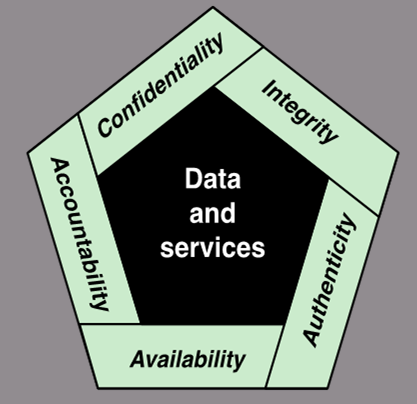
\includegraphics[width=7cm, keepaspectratio]{bistarelli/img/cap_1/cia.png}
	\caption{Requisiti essenziali in Cybersecurity.}\label{fig:cia}
\end{figure}

Sebbene l'uso della triade della CIA per definire gli obiettivi di sicurezza sia ben consolidato,
alcuni nel campo della sicurezza ritengono che siano necessari concetti aggiuntivi da presentare
un quadro completo. Due dei più comunemente citati sono i seguenti:
\begin{itemize}
    \item \textbf{Authenticity} (Autenticità): la proprietà di essere genuini e di poter essere verificati e di essere trusted. Fiducia nella validità di una trasmissione di un messaggio o di un messaggio originatore. Ciò significa verificare che gli utenti siano chi dicono di essere e che ogni input che arriva al sistema proviene da una fonte attendibile.
    \item \textbf{Accountability}(Rendicontabilità): è la capacità di un sistema di identificare un singolo utente, di determinarne le azioni e il comportamento all'interno del sistema stesso. La rendicontabilità è un aspetto del controllo di accesso e si basa sulla concezione che gli individui siano responsabili delle loro azioni all'interno del sistema. Questo supporta il non ripudio, deterrenza, isolamento dei guasti, rilevamento e prevenzione delle intrusioni, il recupero post-azione in concomitanza con l'azione legale . Poiché i sistemi veramente sicuri non sono ancora un obiettivo realizzabile, dobbiamo essere in grado di tracciare una violazione della sicurezza al/ai responsabile/i. I sistemi devono tenere traccia delle loro attività per consentire successive analisi forensi per rintracciare violazioni della sicurezza o per aiutare nelle controversie sulle transazioni.
\end{itemize}
Si noti che FIPS 199 include l'autenticità sotto integrità.
\\
La sicurezza informatica è allo stesso tempo affascinante e complessa, alcuni dei motivi sono:
\begin{enumerate}
    \item \textit{La sicurezza informatica non è così semplice come potrebbe sembrare a un principiante}. I requisiti sembrano essere semplici,in effetti, la maggior parte dei requisiti principali per i servizi di sicurezza possono essere definiti con etichette formate autoesplicative formate da una sola parola: riservatezza, autenticazione, non ripudio e integrità. Ma i meccanismi utilizzati per soddisfare tali requisiti possono essere piuttosto complessi, e capirli può portare a un ragionamento piuttosto sottile.
    \item \textit{Nello sviluppo di un particolare meccanismo di sicurezza o algoritmo, bisogna sempre considerare potenziali attacchi a tali funzionalità di sicurezza.} In molti casi gli attacchi di successo sono progettati guardando un problema in un modo completamente differente, dunque sfruttando una debolezza inaspettata del meccanismo.
    \item \textit{A causa del punto 2 , le procedure usate per fornire dei servizi particolari sono spesso controintuitive.} Tipicamente, un meccanismo di sicurezza è complesso e non è ovvio dalle dichiarazioni di una particolare esigenza che tali misure elaborate sono necessarie. Solo quando si prendono in considerazione i vari aspetti della minaccia si elaborano i meccanismi di sicurezza hanno un senso.
    \item \textit{I meccanismi di sicurezza in genere coinvolgono più di un particolare algoritmo o
    protocollo.}Richiedono inoltre che i partecipanti siano in possesso di un'informazione segreta (ad es. una chiave di crittografia), che sollevano domande sulla creazione, distribuzione e protezione di tali informazioni segrete. Potrebbe esserci anche una dipendenza sui protocolli di comunicazione il cui comportamento può complicare il compito di sviluppare il meccanismo di sicurezza. Ad esempio, se il corretto funzionamento del meccanismo di sicurezza richiede la definizione di limiti di tempo per il tempo di transito di un messaggio dal mittente al destinatario, allora qualsiasi protocollo o rete che introduce variabili e/o ritardi imprevedibili può rendere tali termini privi di significato.
    \item \textit{ La sicurezza informatica è essenzialmente una battaglia di ingegni tra un perpetratore che prova a  trovare buchi e il progettista o l'amministratore che tenta di chiuderli.} Il grande vantaggio che l'attaccante ha è che lei o lui ha solo bisogno di trovare una singola vulnerabilità, mentre il progettista deve trovare e eliminare tutte le vulnerabilità per ottenere una sicurezza perfetta.
    \item \textit{La sicurezza è ancora troppo spesso un'"aggiunta" (surplus) per essere incorporata in un sistema dopo che il progetto è completo, piuttosto che essere parte integrante del processo di progettazione.}
    \item \textit{La sicurezza richiede un monitoraggio regolare, anche costante, e questo è difficile nei tempi attuali.}
    \item \textit{C'è una naturale tendenza da parte di utenti e gestori di sistema a percepire pochi vantaggi nell'investimento sulla sicurezza fino a quando non si verifica un problema.}
    \item \textit{ Molti utenti e persino gli amministratori della sicurezza vedono una sicurezza forte come un ostacolo al funzionamento o all'uso efficiente di un sistema informativo o di un'informazione.}
\end{enumerate}

\subsection{Terminologie}
La maggior parte delle terminologie sono riportate nel Capitolo \ref{ch:terminologie} degli appunti Prof. Santini, di seguito riporto alcuni termini non citati in precedenza.

\subsubsection{Risorsa di sistema (Asset)}
Una applicazione maggiore, un sistema di supporto generale, un programma ad alto impatto,un impianto fisico, un sistema mission-critical, personale, apparecchiature o un gruppo di sistemi logicamente correlati.  

\subsubsection{Minaccia}
Qualsiasi circostanza o evento che potrebbe avere un impatto negativo sulle operazioni organizzative (inclusi missione, funzioni, immagine o reputazione), risorse organizzative, individui, altre organizzazioni o la Nazione stessa attraverso un sistema informativo tramite accesso, distruzione, divulgazione, modifica non autorizzati delle informazioni , e/o negazione del servizio.

\subsubsection{Contromisure}
Dispositivo o tecniche che hanno come obiettivo la compromissione dell'efficacia operativa di attività indesiderate o contraddittorie, o la prevenzione di spionaggio, sabotaggio, furto o accesso o utilizzo non autorizzato di informazioni sensibili o di sistemi informativi.

\subsubsection{Rischio}
Una misura del grado in cui un'entità è minacciata da una potenziale circostanza o evento, e tipicamente una funzione di stima:
\begin{enumerate}
    \item  degli impatti negativi che si verificherebbero se la circostanza o l'evento si verificassero
    \item  della probabilità che si verifichi.
\end{enumerate}

\begin{figure}[H]
	\centering
    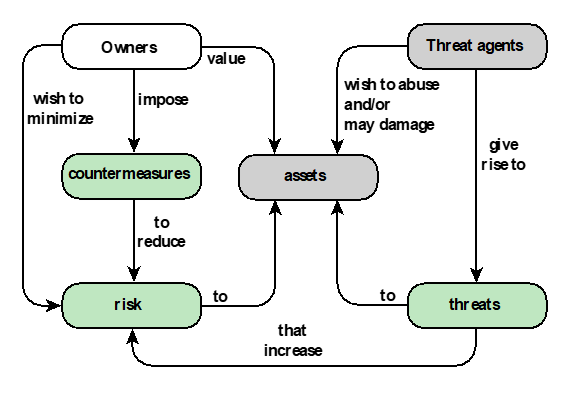
\includegraphics[width=11cm, keepaspectratio]{bistarelli/img/cap_1/relazione_concetti_sicurezza.png}
	\caption{Concetti di sicurezza e le loro relazioni.}\label{fig:relazioni_concetti_sec}
\end{figure}

\subsection{Asset di un sistema informatico}
Gli asset di un sistema informatico possono essere suddivisi come di seguito:
\begin{itemize}
    \item \textbf{Hardware}: compresi i sistemi informatici e altri trattamenti di dati, archiviazione dei dati,e dispositivi di comunicazione dati;
    \item \textbf{Software}: include il sistema operativo, le utilità di sistema e le applicazioni;
    \item \textbf{Data}: inclusi file e database, nonché dati relativi alla sicurezza, ad esempio file di password. 
    \item \textbf{Strutture e reti di comunicazione}: rete locale e geografica collegamenti di comunicazione, bridge, router e così via.
\end{itemize}

\subsection{Vulnerabilità, minacce e attacchi}
Nel contesto della sicurezza, la nostra preoccupazione riguarda le vulnerabilità delle risorse del sistema. [NRC02] elenca le seguenti categorie generali di vulnerabilità di un sistema informatico o di una risorsa di rete:
\begin{itemize}
    \item Il sistema può essere danneggiato (\textbf{corrupted}), quindi fa la cosa sbagliata o dà risposte sbagliate. Ad esempio, i valori dei dati memorizzati possono differire da quello che dovrebbero essere perché sono stati modificati in modo improprio.
    \item Il sistema avere delle perdite (\textbf{be leaky}). Ad esempio, qualcuno che non dovrebbe avere accesso ad alcune o a tutte le informazioni disponibili attraverso la rete ottengono tale accesso.
    \item Il sistema può diventare non disponibile (\textbf{unavailable}) o molto lento. Cioè, usando il sistema o la rete diventa impossibile o impraticabile.
\end{itemize}
Questi tre tipi generali di vulnerabilità corrispondono ai concetti di integrità, riservatezza e disponibilità, enumerati in precedenza. Una \textbf{minaccia} rappresenta un potenziale danno alla sicurezza di una risorsa. Un \textbf{attacco} è una minaccia che viene eseguita (azione di minaccia) e, in caso di successo, comporta una violazione indesiderata della sicurezza o a una conseguenza della minaccia. L'agente che effettua l'attacco viene definito \textbf{attaccante} o \textbf{agente di minaccia}. Possiamo distinguere gli attacchi in due tipi:
\begin{itemize}
    \item \textbf{Attacco attivo}: un tentativo di alterare le risorse del sistema o di influenzare il funzionamento.
    \item \textbf{Attacco passivo}: un tentativo di imparare o di fare use delle informazioni da un sistema che non influenza le risorse di quest'ultimo.
\end{itemize}

\noindent
Possiamo classificare gli attacchi in base all'origine di questi:
\begin{itemize}
    \item \textbf{Attacco interno}: iniziato da un entità interna al perimetro di sicurezza ( un "insider"). L'insider è autorizzato all'accesso alle risorse del sistema ma le usa in un modo non approvato da coloro che ne garantiscono l'accesso.  
    \item \textbf{Attacco esterno}: iniziato fuori dal perimetro, da un utente non autorizzato o illegittimo del sistema (un "outsider"). Su Internet, potenziale aggressori esterni variano dai dilettanti "burloni" a criminali organizzati, internazionali terroristi e governi ostili.
\end{itemize}

Infine, una contromisura è qualsiasi mezzo adottato per affrontare un attacco alla sicurezza. Idealmente, una contromisura può essere escogitata per prevenire un particolare tipo di attacco dall'avere successo. Quando la prevenzione non è possibile, o in alcuni casi fallisce, l'obiettivo è rilevare l'attacco e poi riprendersi dagli effetti . Una contromisura stessa può introdurre nuove vulnerabilità. In ogni caso, vulnerabilità residue
possono rimanere dopo l'imposizione di contromisure. Tali vulnerabilità possono essere sfruttato da attaccanti che rappresentano un livello di rischio residuo per gli asset. I proprietari dell'asset cercheranno di ridurre al minimo tale rischio dati altri vincoli.


\begin{figure}[H]
	\centering
    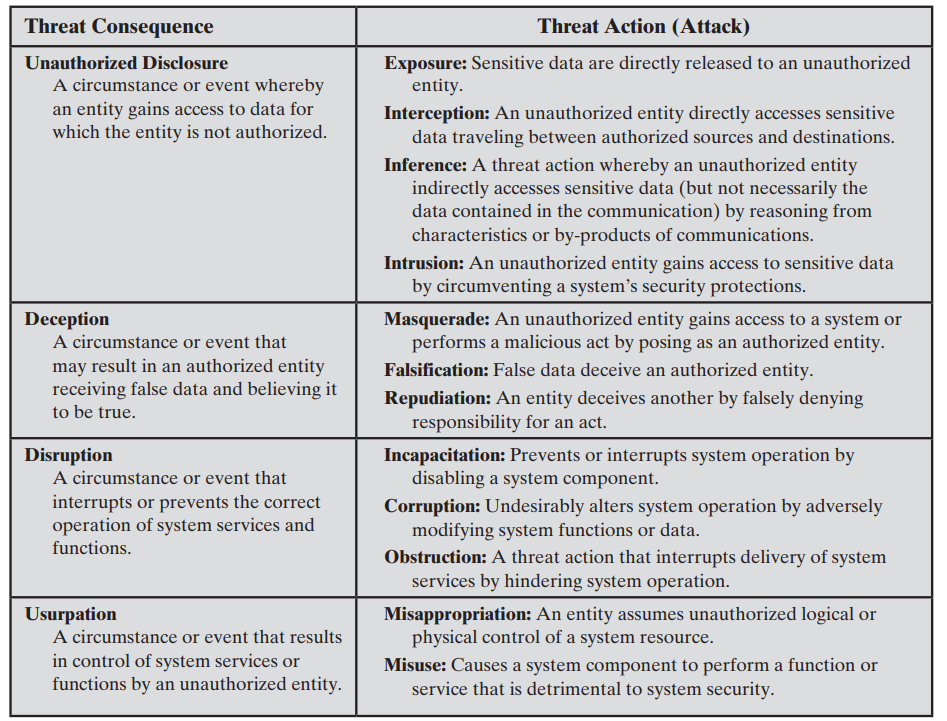
\includegraphics[width=14cm, keepaspectratio]{bistarelli/img/cap_1/tabella_minacce.png}
	\caption{Conseguenze delle minacce e azioni che le causano }\label{fig:tabella_minacce}
\end{figure}

La tabella \ref{fig:tabella_minacce} basata su RFC 4949, descrive quattro tipi di conseguenze ed elenca i tipi di attacchi che risultano in ciascuna conseguenza. 

La divulgazione non autorizzata (Unauthorized disclosure) è una minaccia alla riservatezza. I seguenti tipi di attacchi possono portare a queste conseguenze

\begin{itemize}
    \item \textbf{Esposizione}: quando un insider rilascia intenzionalmente informazioni sensibili a un estraneo, come ad esempio i numeri di carta di credito. Può anche essere il risultato di un errore umano, hardware o software, che si traduce nell'azione da parte di un'entità di avere l'accesso non autorizzato di dati sensibili. Ce ne sono stati numerosi casi di questo, come le università che pubblicano accidentalmente le informazioni confidenziali degli studenti sul Web.
    \item \textbf{Intercettazione}: l'intercettazione è un attacco comune nel contesto delle comunicazioni. Su una rete locale condivisa (LAN), come una LAN wireless o a broadcast Ethernet, qualsiasi dispositivo collegato alla LAN può ricevere una copia dei pacchetti destinati a un altro dispositivo. Su Internet, un determinato hacker può accedere al traffico di posta elettronica e ad altri trasferimenti di dati. Tutte queste situazioni possono portare all'accesso non autorizzato ai dati.
    \item \textbf{Inferenza}: un esempio di inferenza è noto come analisi del traffico, in cui un avversario è in grado di ottenere informazioni osservando l'andamento del traffico una rete, come la quantità di traffico tra particolari coppie di host sulla rete. Un altro esempio è l'inferenza di informazioni dettagliate da un database di un utente che ha solo un accesso limitato, questo è realizzato da query ripetute i cui risultati combinati consentono l'inferenza.
    \item \textbf{Intrusione}: un esempio di intrusione è un avversario che ottiene l'accesso non autorizzato a dati sensibili superando le protezioni di controllo degli accessi del sistema.
\end{itemize}

L'inganno (Deception) è una minaccia per l'integrità del sistema o per l'integrità dei dati. I seguenti tipi di attacchi possono portare a queste conseguenze:
\begin{itemize}
    \item \textbf{Masquerade}: un esempio di masquerade è un tentativo di accesso a un sistema  da parte di un utente non autorizzato spacciandosi per uno autorizzato, questo può succedere se l'utente non autorizzato conosce l'ID di accesso e la password di un altro utente. Un altro esempio è la logica dannosa (malicious logic), come un cavallo di Troia, che appare per eseguire una funzione utile o desiderabile, ma in realtà ottiene l'accesso non autorizzato alle risorse di sistema o induce un utente a eseguire altre logiche dannose.
    \item \textbf{Falsificazione}: si riferisce all'alterazione o sostituzione di dati validi o all'introduzione di dati falsi in un file o database. Ad esempio, uno studente può alterare i suoi voti su un database scolastico.
    \item \textbf{Ripudio}: in questo caso, un utente nega l'invio di dati o nega di ricevere o possedere i dati.
\end{itemize}

L'interruzione (Disruption) è una minaccia alla disponibilità o all'integrità del sistema. I seguenti tipi di attacchi possono portare a queste conseguenze:
\begin{itemize}
    \item \textbf{Incapacità}: questo è un attacco alla disponibilità del sistema. Ciò potrebbe verificarsi come risultato della distruzione fisica o del danneggiamento dell'hardware del sistema. Più tipicamente, un software dannoso, come Trojan, virus o worm, potrebbero operarein modo tale da disabilitare un sistema o alcuni dei suoi servizi.
    \item \textbf{Corruzione}: questo è un attacco all'integrità del sistema. Un Software dannoso in questo contesto potrebbe funzionare in modo tale che le risorse di sistema o i servizi funzionino in modo non intenzionale. Oppure un utente potrebbe ottenere l'accesso non autorizzato a un sistema e modificarne alcune funzioni. Un esempio di quest'ultimo è un posizionamento di una logica backdoor (backdoor logic) nel sistema per fornire il successivo accesso al sistema stesso e alle sue risorse con una procedura diversa da quella abituale.
    \item \textbf{Ostruzione}: un modo per ostacolare il funzionamento del sistema è interferire con le comunicazioni disabilitando i collegamenti di comunicazione o alterando la comunicazione delle informazioni di controllo. Un altro modo è sovraccaricare il sistema mettendo un carico in eccesso sul traffico di una comunicazione o sulle risorse di elaborazione.
\end{itemize}

L'usurpazione (Usurpation) è una minaccia per l'integrità del sistema. I seguenti tipi di attacchi possono portare a queste conseguenze:
\begin{itemize}
    \item \textbf{Appropriazione indebita}: può includere il furto del servizio. Un esempio è un attacco Denial of Service distribuito, quando il software dannoso è installato su degli host da utilizzare come piattaforme per avviare il traffico verso un host di destinazione. In questo caso, il software maligno fa uso non autorizzato delle risorse del processore e del sistema operativo.
    \item \textbf{Uso improprio}: l'uso improprio può verificarsi per mezzo di una malicious logic o di un hacker che ha ottenuto un accesso non autorizzato a un sistema. In entrambi i casi, le funzioni di sicurezza possono essere disabilitate o contrastate.
\end{itemize}

\subsection{Asset e minacce}
Le risorse di un sistema informatico possono essere classificate come hardware, software, dati, linee e reti di comunicazione. In questa sottosezione li descriviamo brevemente e mettendoli in relazione con i concetti di integrità, riservatezza e
disponibilità. 

\begin{figure}[H]
	\centering
    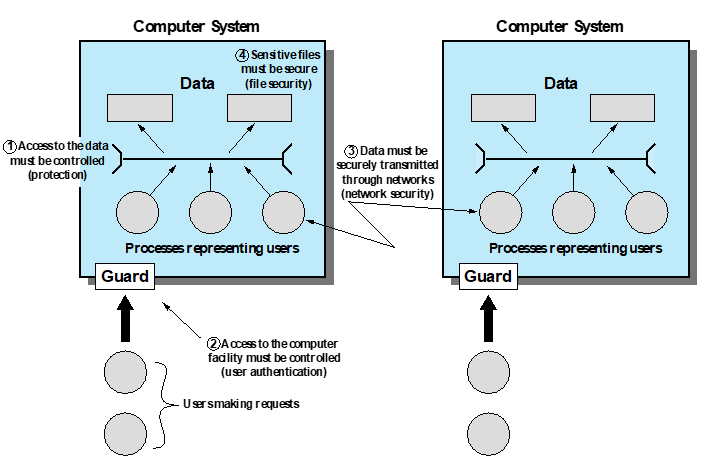
\includegraphics[width=14cm, keepaspectratio]{bistarelli/img/cap_1/asset_sec.png}
	\caption{ Scopo della sicurezza informatica.}\label{fig:asset_sec}
\end{figure}

\paragraph{Hardware.} Una delle principali minacce per l'hardware  del computer è la minaccia alla disponibilità. L'hardware è il più vulnerabile agli attacchi e il meno suscettibile ai controlli automatizzati. Le minacce includono danni accidentali e deliberati alle apparecchiature così come il furto. La proliferazione di personal computer e workstation e l'uso diffuso delle LAN aumenta il potenziale di perdite in quest'area. Il furto delle unità USB può portare alla perdita di riservatezza. Le misure di sicurezza fisiche e amministrative sono necessarie per far fronte a queste minacce.


\paragraph{Software.} Il software include il sistema operativo, le utilità e l'applicazione programmi. Una delle principali minacce al software è un attacco alla disponibilità. Il Software, in particolare quello applicativo, è spesso facile da eliminare. Il software può anche essere modificato o danneggiato per renderlo inutilizzabile. Un'attenta gestione della configurazione del software, che include il mantenere dei backup della versione più recente, può mantenere una disponibilità alta. Un problema più difficile da affrontare è la modifica del software che si ha in un programma il quale funziona ancora ma che si comporta in modo diverso rispetto a prima,
questa è una minaccia per l'integrità/autenticità. Rientrano in questa categoria i virus informatici e i relativi attacchi. Un ultimo problema è la protezione contro la pirateria del software. Sebbene siano disponibili alcune contromisure, in linea di massima il problema di copie non autorizzate del software non è stata risolta.

\paragraph{Data.}  Un  problema molto più diffuso è la sicurezza dei dati, che coinvolge file e altre forme di dati controllati da individui, gruppi e organizzazioni aziendali.

I problemi di sicurezza relativi ai dati sono ampi e comprendono disponibilità, segretezza e integrità. In caso di disponibilità, la preoccupazione è con la distruzione di file di dati, che può verificarsi accidentalmente o intenzionalmente. 
Una preoccupazione evidente per la segretezza è la lettura non autorizzata di file di dati o database, e quest'area è stata forse oggetto di ulteriori ricerche e sforzi rispetto a qualsiasi altro settore della sicurezza informatica. Una minaccia meno ovvia alla segretezza comporta l'analisi dei dati e si manifesta nell'utilizzo delle cosiddette banche dati statistiche, che forniscono informazioni di sintesi o aggregate. Presumibilmente, l'esistenza delle informazioni aggregate non minacciano la privacy delle persone coinvolte. Tuttavia, con la crescita dell'uso delle banche dati statistiche, c'è un rischio crescente per la divulgazione di informazioni personali. In sostanza, le caratteristiche di un individuo possono essere identificate attraverso un'analisi attenta. Ad esempio, se una tabella registra l'aggregato dei redditi degli intervistati A, B, C e D e un altro registra l'aggregato dei redditi di A, B, C, D ed E, la differenza tra i due aggregati sarebbe il reddito di E. Questo problema è esasperato dal desiderio crescente di combinare set di dati. In molti casi, abbinando diversi set di dati per coerenza tra i diversi livelli di aggregazione è necessario l'accesso alle singole unità. Pertanto, le singole unità, che sono oggetto di problemi di privacy, sono disponibili in varie fasi del trattamento dei set di dati. 
Infine, l'integrità dei dati è una delle principali preoccupazioni nella maggior parte delle installazioni.Le modifiche ai file di dati possono avere conseguenze che vanno da minori a disastrose.

\subsection{Attacchi passivi e attivi}
Gli attacchi alla sicurezza della rete possono essere classificati
come attacchi passivi e attacchi attivi. Un attacco passivo tenta di imparare o fare
uso delle informazioni del sistema, ma non influisce sulle risorse di quest'ultimo. Un attacco attivo tenta di alterare le risorse di sistema o di influenzare il loro funzionamento.

\subsubsection{Attacchi passivi}
Gli \textbf{attacchi passivi} generalmente riguardano l'intercettazione o il monitoraggio di trasmissioni di dati. L'obiettivo dell'attaccante è ottenere le informazioni che vengono trasmesse. Due tipi di attacchi passivi sono il rilascio del contenuto dei messaggi e dell'analisi del traffico.

\paragraph{Rilascio dei contenuti di un messaggio} Il \textbf{rilascio dei contenuti} del messaggio è facilmente comprensibile. Una conversazione telefonica, un messaggio di posta elettronica e un file trasferito possono contenere dati sensibili o informazioni confidenziali. Vorremmo impedire a un avversario di imparare il contenuto di queste trasmissioni.

\paragraph{Analisi del traffico.} Un secondo tipo di attacco passivo, \textbf{l'analisi del traffico}, è più sottile. Supponiamo che noi abbiamo un modo per mascherare il contenuto dei messaggi o altre informazioni del traffico di dati, in modo che gli oppositori, anche se hanno catturato il messaggio, non possono estrarre le informazioni dal messaggio. La tecnica comune per mascherare i contenuti è la crittografia. Anche se disponiamo di una protezione crittografica, un avversario potrebbe comunque essere in grado di osservare lo schema di questi messaggi. L'avversario potrebbe determinare la posizione e l'identità degli host nella comunicazione e potrebbe osservare la frequenza e la lunghezza dei messaggi scambiati. Queste informazioni potrebbero essere utili per indovinare la natura della comunicazione che stava avvenendo.

Gli attacchi passivi sono molto difficili da rilevare perché non coinvolgono alterazione dei dati. In genere, il traffico dei messaggi viene inviato e ricevuto in un modo apparentemente normale e né il mittente né il destinatario sono consapevoli che una terza parte ha letto i messaggi o osservato l'andamento del traffico. Tuttavia, è possibile prevenire il successo di questi attacchi, di solito mediante crittografia. Pertanto, l'enfasi nell'affrontare gli attacchi passivi è sulla prevenzione piuttosto che il rilevamento.

\subsubsection{Attacchi attivi}
Gli attacchi attivi comportano alcune modifiche del flusso di dati o la creazione
di un falso flusso, esso può essere suddiviso in quattro categorie: replay, masquerade, modifica dei messaggi e denial of service.

\paragraph{Replay.} Il replay comporta l'acquisizione passiva di un'unità di dati e la sua successiva ritrasmissione per produrre un effetto non autorizzato.


\paragraph{Masquerade.} Una masquerade ha luogo quando un'entità finge di essere un'entità diversa. Un attacco di questo tipo di solito include una delle altre forme di attacco attivo. Per esempio, le sequenze di autenticazione possono essere catturate e riprodotte dopo che è avvenuta una sequenza di autenticazione valida, abilitando così un'entità autorizzata con pochi privilegi a ottenere privilegi extra impersonando un'entità che dispone di tali privilegi.

\paragraph{Modifica di un messaggio.} La modifica dei messaggi significa semplicemente che una parte di un legittimo messaggio è alterato, o che i messaggi sono ritardati o riordinati, per produrre un effetto non autorizzato. Ad esempio, un messaggio che afferma: "Consenti a John Smith di leggere dati di file riservati" viene modificato per dire "Consenti a Fred Brown di leggere dati di file riservati".

\paragraph{DOS.} La negazione del servizio impedisce o inibisce il normale utilizzo o gestione delle strutture di comunicazione. Questo attacco può avere un obiettivo specifico, per esempio un'entità può sopprimere tutti i messaggi diretti a una particolare destinazione (ad esempio, la sicurezza del servizio di audit). Un'altra forma di rifiuto del servizio è l'interruzione di un'intera rete, o disabilitando la rete o sovraccaricandola di messaggi in modo da degradarne le prestazioni.

Gli attacchi attivi presentano le caratteristiche opposte degli attacchi passivi. Invece gli attacchi passivi sono difficili da rilevare, sono disponibili misure per prevenirli con successo. D'altra parte, è abbastanza difficile prevenire assolutamente gli attacchi attivi, perché per farlo richiederebbe la protezione fisica di tutte le strutture e i percorsi di comunicazione in ogni momento. Invece, l'obiettivo è rilevarli e riprendersi da qualsiasi disservizio o ritardi da essi causati. Poiché il rilevamento ha un effetto deterrente, esso può anche contribuire alla prevenzione.

\subsection{Requisiti di sicurezza} 
Esistono diversi modi per classificare e caratterizzare le contromisure che possono essere utilizzate per ridurre le vulnerabilità e affrontare le minacce alle risorse di sistema. In questa sottosezione, vediamo contromisure in termini di requisiti funzionali, e seguiamo la classificazione definita in FIPS 200. Questo standard enumera 17 aree relative alla sicurezza con riguardo alla protezione della riservatezza, dell'integrità e della disponibilità delle informazioni di sistemi e le informazioni elaborate, archiviate e trasmesse da tali sistemi.
\begin{enumerate}
    \item \textbf{Accesso controllato}: limitare l'accesso al sistema informativo agli utenti autorizzati, ai processi che agiscono per conto degli utenti autorizzati, o ai dispositivi (inclusi altri sistemi informativi) e alle tipologie di transazioni e funzioni che gli utenti autorizzati possono esercitare.
    \item \textbf{Consapevolezza e Formazione}: garantire che i gestori e gli utenti dei sistemi informativi organizzativi siano consapevole dei rischi per la sicurezza associati alle proprie attività e delle leggi, dei regolamenti e delle politiche applicabili relativi alla sicurezza dei sistemi informativi organizzativi e  garantire che il personale sia adeguatamente addestrato a svolgere i compiti e le responsabilità assegnate in materia di sicurezza delle informazioni.
    \item \textbf{Audit e responsabilità}: creare, proteggere e conservare i record di audit del sistema informativo per consentire il monitoraggio, l'analisi, l'indagine e la segnalazione di atti illeciti, non autorizzati o di attività non appropriate del sistema informativo. Garantire inoltre che le azioni dei singoli individui  nel sistema possano essere ricondotte in modo univoco a tali utenti in modo che possano essere ritenuti responsabili di esse.
    \item \textbf{Certificazione, accreditamento e valutazioni di sicurezza}: valutare periodicamente i controlli di sicurezza nei sistemi informativi organizzativi per determinare se i controlli sono efficaci nella loro applicazione. Sviluppare e attuare piani d'azione volti a correggere le carenze e ridurre o eliminare le vulnerabilità in questi sistemi. Autorizzare l'esercizio dei sistemi informativi organizzativi ed eventuali connessioni associate a questi. Monitorare continuamente i controlli di sicurezza del sistema informativo  per garantire la continua efficacia di essi.
    \item \textbf{Gestione della configurazione}: stabilire e mantenere le configurazioni di base e gli inventari dei sistemi (inclusi hardware, software, firmware e documentazione) durante i rispettivi cicli di vita di sviluppo del sistema. Stabilire e far rispettare le impostazioni di configurazione di sicurezza per i prodotti informatici utilizzati nei sistemi.
    \item \textbf{Pianificazione di emergenza}: stabilire, mantenere e implementare piani di risposta alle emergenze, operazioni di backup, e il ripristino post-disastro per i sistemi in modo da garantire la disponibilità di risorse informative critiche e continuità operativa in situazioni di emergenza.
    \item \textbf{Identificazione e autenticazione}: identificare gli utenti del sistema, i processi che agiscono per conto degli utenti o dei dispositivi e autenticare (o verificare) le identità di tali utenti, processi o dispositivi, come prerequisito per consentire l'accesso ai sistemi.
    \item \textbf{Risposta all'incidente}: stabilire una capacità operativa di gestione degli incidenti per le informazioni organizzative dei sistemi che includono un'adeguata preparazione, rilevamento, analisi, contenimento, recupero e un controllo delle attività di risposta dell'utente. Tracciare, documentare e segnalare gli incidenti ai funzionari appropriati e/o alle autorità.
    \item \textbf{Manutenzione}: eseguire la manutenzione periodica e tempestiva dei sistemi, fornire controlli efficaci sugli strumenti, sulle tecniche, sui meccanismi e sul personale utilizzato per condurre una manutenzione del sistema informativo.
    \item \textbf{Protezione dei media}: proteggere i media dei sistemi, sia cartacei che digitali, limitare l'accesso alle informazioni dei media agli utenti autorizzati e sanificare o distruggere prima i supporti del sistema informativo prima dello smaltimento o del rilascio per il riutilizzo.
    \item \textbf{Protezione fisica e ambientale}: limitare l'accesso fisico dei soggetti autorizzati ai sistemi informativi, alle apparecchiature e ai rispettivi ambienti operativi. Proteggere l'impianto fisico e l' infrastruttura di supporto per i sistemi. Fornire utilità di supporto per i sistemi informativi e proteggere quest'ultimi dai rischi ambientali fornendo adeguati controlli ambientali alle strutture che li contengono.
    \item \textbf{Pianificazione}: sviluppare, documentare, aggiornare periodicamente e implementare piani di sicurezza per le informazioni organizzative dei sistemi che descrivono i controlli di sicurezza esistenti o previsti e le regole di comportamento dei soggetti che accedono ai sistemi.
    \item \textbf{Sicurezza del personale}: garantire che le persone che occupano posizioni di responsabilità all'interno delle organizzazioni (compresi i fornitori di servizi di terze parti) siano affidabili e soddisfino i criteri di sicurezza stabiliti per quelle posizioni. Garantire che le informazioni organizzative e i sistemi informativi siano protetti durante e dopo le azioni del personale quali licenziamenti e trasferimenti. Applicare sanzioni formali per il personale che non fa rispettare le politiche e le procedure di sicurezza dell'organizzazione.
    \item \textbf{Valutazione del rischio}: valutare periodicamente il rischio per le operazioni organizzative (inclusi missioni, funzioni, immagine o reputazione), risorse organizzative e individui, risultanti dal funzionamento del sistema e il relativo trattamento, archiviazione o trasmissione di informazioni organizzative.
    \item \textbf{Acquisizione di sistemi e servizi}: Allocare risorse sufficienti per proteggere adeguatamente l'organizzazione dei sistemi. Impiegare processi del ciclo di vita dello sviluppo del sistema che incorporano considerazioni sulla sicurezza. Imporre limitazioni all'utilizzo e all'installazione del software e garantire che i fornitori di terze parti adottino adeguate misure di sicurezza per proteggere le informazioni, le applicazioni e/o i servizi "esternalizzati" dall'organizzazione.
    \item \textbf{Protezione del sistema e delle comunicazioni}: monitorare, controllare e proteggere le comunicazioni organizzative (vale a dire, le informazioni trasmesse o ricevute dai sistemi) ai confini esterni e interni. Impiegare progetti "architettonici", sviluppo software tecniche e principi di ingegneria dei sistemi che promuovono un'efficace sicurezza delle informazioni all'interno di dei sistemi organizzativi.
    \item \textbf{Integrità del sistema e delle informazioni}: identificare, segnalare e correggere le informazioni e le falle del sistema in modo tempestivo. Fornire protezione da codice dannoso in posizioni appropriate all'interno del sistema organizzativo e monitorare gli avvisi di sicurezza del sistema informativo e adottare le azioni appropriate in risposta.
\end{enumerate}
    \chapter{Capitolo 2}
\section{Riservatezza con la crittografia simmetrica}
Una delle tecniche per garantire la riservatezza dei dati trasmessi o memorizzati è la crittografia simmetrica.
Segue una panoramica dei due più importanti algoritmi di crittografia simmetrica: 

\begin{itemize}
    \centering
    \item \textbf{Il Data Encryption Standard (Standard di Crittografia dei Dati)} (DES)
    
    \item \textbf{L'Advanced Encryption Standard} (AES) 
\end{itemize}

Che sono algoritmi di crittografia a blocchi, ma esiste anche il concetto di crittografia a flusso.

\newpage
\subsection{Crittografia Simmetrica}

\begin{figure}[H]
	\centering
    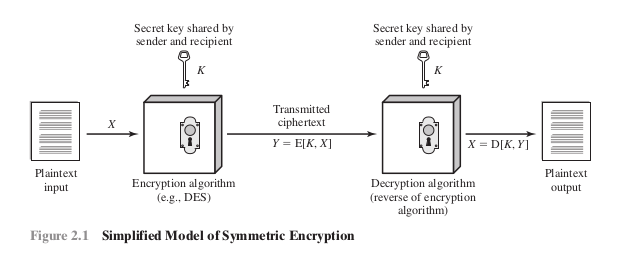
\includegraphics[width=14cm, keepaspectratio]{Bistarelli/img/cap_2/figura2.1.png}
\end{figure}

Uno schema di crittografia simmetrica ha cinque ingredienti (vedi Figura 2.1):
\begin{itemize}
    \item \textbf{Testo in chiaro:} Si tratta del messaggio o dei dati originali che vengono inseriti nell'algoritmo come in ingresso.
    
    \item \textbf{Algoritmo di crittografia:} L'algoritmo di crittografia esegue varie sostituzioni e trasformazioni sul testo in chiaro.
    
    \item \textbf{Chiave segreta:} La chiave segreta che è l'input dell'algoritmo di crittografia. 
    
    \item \textbf{Testo cifrato:} È il messaggio criptato prodotto in uscita. 
    
    Dipende dal testo in chiaro e dalla chiave segreta. Per un dato messaggio, due chiavi diverse produrranno due cifrari diversi.
    
   \item \textbf{Algoritmo di decifrazione:} Si tratta essenzialmente dell'algoritmo di crittografia eseguito  all'inverso. 
    
    Prende il testo cifrato e la chiave segreta e produce il testo in chiaro originale.
\end{itemize}
\newpage
I requisiti per un \textbf{uso sicuro della crittografia simmetrica} sono due:
\begin{enumerate}
    \item \textbf{È necessario un algoritmo di crittografia forte.}
    
   Se un avversario conosce l'algoritmo di cifratura ed ha accesso a uno o più testi cifrati non deve comunque essere in grado di decifrarli.
    
    \item \textbf{Il mittente e il destinatario devono aver ottenuto copie della chiave segreta in modo sicuro e devono mantenerla protetta.}
    
    Se qualcuno scopre la chiave e conosce l'algoritmo, tutte le comunicazioni che utilizzano la medesima chiave sono leggibili.
\end{enumerate}
Esistono due approcci generali per attaccare uno schema di crittografia simmetrica.
\paragraph{Il primo attacco} è noto come crittoanalisi. Gli attacchi di crittoanalisi si basano sulla natura dell'algoritmo e sulla conoscenza delle caratteristiche generali del testo in chiaro e del testo cifrato. 

\singlespacing

Questo tipo di attacco sfrutta le caratteristiche dell'algoritmo per cercare di dedurre un testo in chiaro specifico o di dedurre la chiave utilizzata. Se l'attacco riesce a dedurre la chiave, l'effetto è catastrofico: \textbf{Tutti i messaggi futuri e passati crittografati con quella chiave sono compromessi.}

\singlespacing

\paragraph{Il secondo metodo} noto come attacco a forza bruta, consiste nel provare ogni possibile chiave su un pezzo di testo cifrato finché non si ottiene una traduzione comprensibile in testo in chiaro. In media, la metà di tutte le chiavi possibili deve essere provata per ottenere un successo. Cioè, se ci sono x chiavi diverse, in media un attaccante scoprirebbe la chiave effettiva dopo $x/2$ tentativi.

\subsection{Algoritmi di crittografia a blocchi simmetrici}
Gli algoritmi di crittografia simmetrica più utilizzati sono \textbf{i cifrari a blocchi.} 

\singlespacing

Un cifrario a blocchi elabora il testo in chiaro in blocchi di dimensioni fisse e produce un blocco di testo cifrato di dimensioni uguali per ogni blocco di testo in chiaro. L'algoritmo elabora quantità di testo in chiaro come una serie di blocchi di dimensioni fisse. Gli algoritmi simmetrici più importanti, che sono tutti cifrari a blocchi, sono il Data Encryption Standard (DES), il triplo DES e l'Advanced Encryption Standard (AES)

\begin{figure}[H]
	\centering
    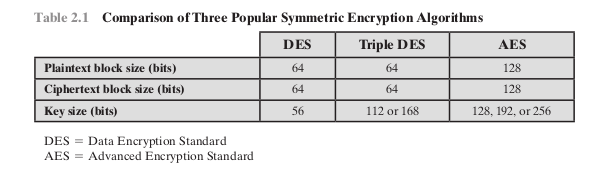
\includegraphics[width=14cm, keepaspectratio]{Bistarelli/img/cap_2/tabella2.1.png}
\end{figure}


Vedi tabella 2.1

\paragraph{DES} Fino a poco tempo fa, lo schema di crittografia più diffuso era basato sul Data Encryption Standard (DES). Il DES utilizza un blocco di testo in chiaro di 64 bit e una chiave di 56 bit per produrre un blocco di testo cifrato di 64 bit. I problemi del DES si dividono in due categorie: 

\begin{itemize}
    \item Problemi sull'algoritmo stesso
    
    \item Problemi sull'uso di una chiave a 56 bit. 
\end{itemize}
\paragraph{Il primo problema:} si riferisce alla possibilità che la crittoanalisi sia possibile sfruttando le caratteristiche dell'algoritmo DES. Nel corso degli anni, ci sono stati numerosi tentativi di trovare e sfruttare le debolezze dell'algoritmo, rendendo il DES l'algoritmo di crittografia più studiato in assoluto. Nonostante i numerosi approcci, finora nessuno ha segnalato una debolezza "cruciale" nel DES.

\singlespacing

\paragraph{IL secondo problema è la lunghezza della chiave.} Con una lunghezza di 56 bit, ci sono 256 chiavi possibili, pari a circa 7,2 * 1016 chiavi. Considerata la velocità dei processori in commercio, questa lunghezza di chiave è tristemente inadeguata. Un documento di Seagate Technology suggerisce che una velocità di un miliardo (109) di combinazioni di chiavi al secondo è ragionevole per gli attuali computer multicore. Le offerte recenti lo confermano. Sia Intel che AMD offrono ora istruzioni basate su hardware per accelerare l'uso di AES. I test condotti su una macchina Intel multicore contemporanea hanno dato come risultato una velocità di crittografia di circa mezzo miliardo di chiavi al secondo. Un'altra recente analisi suggerisce che, con la tecnologia contemporanea dei supercomputer, una velocità di 1013 crittografie/s è ragionevole.

\singlespacing

Tenendo conto di questi risultati, la Tabella 2.2 mostra quanto tempo è necessario per compiere un attacco di forza bruta per chiavi di varie dimensioni. Come si può notare, un singolo PC può violare il DES in circa un anno. Se più PC lavorano in parallelo, il tempo si riduce drasticamente. I supercomputer di oggi dovrebbero essere in grado di trovare una chiave in circa un'ora. Le chiavi di dimensioni 128 bit o superiori sono di fatto inviolabili con un semplice approccio di forza bruta. Anche se riuscissimo a velocizzare il sistema di attacco di un fattore di 1 trilione (1012), ci vorrebbero comunque più di 100.000 anni per decifrare un codice che utilizza una chiave a 128 bit. Fortunatamente esistono diverse alternative al DES, le più importanti delle quali sono il triplo DES e l'AES.

\singlespacing

\paragraph{TripleDes} La vita del DES è stata prolungata dall'uso del triple DES (3DES), che prevede \textbf{la ripetizione dell'algoritmo DES di base per tre volte} utilizzando due o tre chiavi uniche, per una dimensione della chiave di 112 o 168 bit. Il 3DES è stato standardizzato per la prima volta per l'uso in applicazioni finanziarie nello standard ANSI X9.17 nel 1985. Il 3DES ha due caratteristiche che ne assicurano la diffusione nei prossimi anni.

\begin{itemize}
    \item Grazie alla lunghezza della chiave di 168 bit, supera la vulnerabilità agli attacchi di forza bruta del DES.
    
    \item L'algoritmo di crittografia sottostante al 3DES è lo stesso del DES.
\end{itemize}

Questo algoritmo è stato sottoposto a maggiori controlli rispetto a qualsiasi altro algoritmo di crittografia per un periodo di tempo più lungo e non è stato trovato alcun attacco di crittoanalisi efficace basato sull'algoritmo piuttosto che sulla forza bruta. Di conseguenza, c'è un'elevato livello di fiducia che il 3DES sia molto resistente alla crittoanalisi.

\singlespacing

\textbf{Il principale svantaggio} del 3DES è che l'algoritmo è relativamente lento nel software. Il 3DES, che richiede un numero di calcoli tre volte i calcoli del DES, è di conseguenza più lento. Un altro svantaggio è che sia il DES che il 3DES utilizzano una dimensione di blocco di 64 bit. Per ragioni di efficienza e sicurezza, è auspicabile una dimensione di blocco maggiore.

\singlespacing

\paragraph{AES} A causa dei suoi svantaggi, il 3DES non è un candidato ottimale per un uso a lungo termine.
Per sostituirlo, nel 1997 il NIST ha pubblicato un invito a presentare proposte per un nuovo Advanced Encryption Standard (AES), che dovrebbe avere una forza di sicurezza pari o superiore al 3DES e un'efficienza sicurezza pari o superiore al 3DES ma sicuramente un'efficienza significativamente migliorata.

\singlespacing

Oltre a questi requisiti generali, il NIST ha specificato che AES deve essere un cifrario a blocchi simmetrico con un blocco simmetrico con una lunghezza di blocco di 128 bit e supporto per chiavi di 128, 192 e 256 bit. 
I criteri di valutazione includevano \textbf{la sicurezza, l'efficienza computazionale, requisiti di memoria, idoneità hardware e software e flessibilità.} In una prima fase di valutazione sono stati accettati 15 algoritmi proposti. In un secondo momento si è poi ristretto il campo a 5 algoritmi. Il NIST ha completato il processo di valutazione e ha pubblicato lo standard finale come FIPS PUB 197 (Advanced Encryption Standard, novembre 2001). 

\subsection{Cifrari a flusso}
Un cifrario a blocchi elabora l'input un blocco di elementi alla volta, producendo un blocco di output per ogni blocco di input. Un cifrario a flusso elabora gli elementi in ingresso in modo continuo, producendo un elemento in uscita alla volta, man mano che procede. Sebbene i cifrari a blocchi siano molto più comuni, ci sono alcune applicazioni in cui un cifrario a flusso è più appropriato. Un tipico cifrario a flusso cripta il testo in chiaro un byte alla volta, anche se un cifrario a flusso può essere progettato per operare su un bit alla volta o su unità di dimensioni pi\`{u} grandi di un byte alla volta.

\begin{figure}[H]
	\centering
    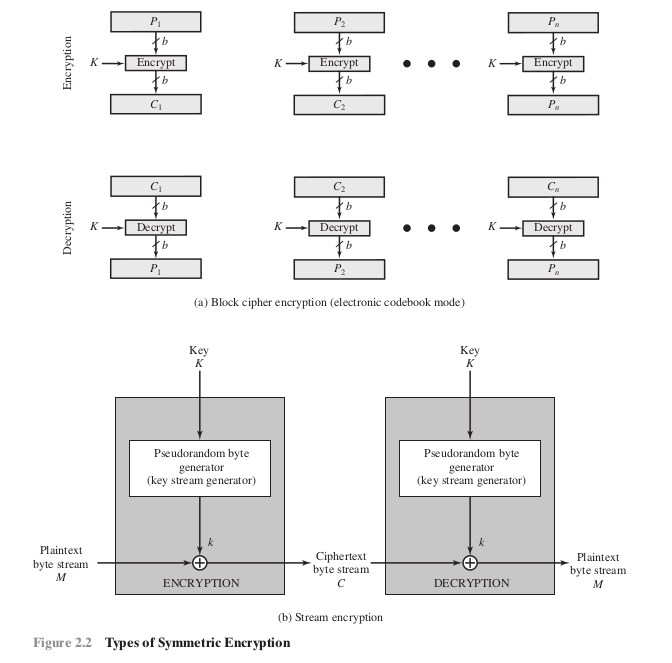
\includegraphics[width=14cm, keepaspectratio]{Bistarelli/img/cap_2/figura2.2.png}
\end{figure}

La Figura 2.2b è un diagramma rappresentativo della struttura di un cifrario a flusso. 

\singlespacing

In questa struttura, una chiave viene immessa in un generatore di bit pseudorandom che produce un flusso di numeri a 8 bit che sono apparentemente casuali. Un flusso pseudorandom è un flusso imprevedibile senza conoscere la chiave di ingresso e che ha un carattere apparentemente casuale. L'output del generatore, chiamato flusso di chiavi, viene combinato un byte alla volta con il flusso di testo in chiaro utilizzando l'operazione di OR esclusivo bitwise (XOR). Con un generatore di numeri pseudorandom correttamente progettato, un cifrario a flusso può essere sicuro quanto un cifrario a blocchi di lunghezza analoga. Il vantaggio principale di un cifrario a flusso è che i cifrari a flusso sono quasi sempre più veloci e utilizzano molto meno codice rispetto ai cifrari a blocco in più è possibile riutilizzare le chiavi. Per applicazioni che richiedono la crittografia/decrittografia di un flusso di dati, come ad esempio un canale di comunicazione dati o un browser/Web. Un cifrario a flusso potrebbe essere l'alternativa migliore. Per le applicazioni che trattano blocchi di dati, come il trasferimento di file, e-mail e database, i cifrari a blocchi possono essere più appropriati. Tuttavia, entrambi i tipi di di cifratura possono essere utilizzati praticamente in qualsiasi applicazione.
\section{Autenticazione basata su messaggio e funzioni Hash}
La crittografia protegge sia dagli \textbf{attacchi passivi} (intercettazioni) che dagli \textbf{attacchi attivi} (falsificazione di dati e transazioni). 

\singlespacing

La protezione contro tali attacchi è nota come autenticazione dei messaggi o dei dati. Un messaggio, un file, un documento o un'altra raccolta di dati si dice autentico quando è genuino e proviene dalla sua presunta fonte. L'autenticazione dei messaggi o dei dati è una procedura che consente alle parti comunicanti di verificare \textbf{che i messaggi ricevuti o memorizzati siano autentici.}

\singlespacing

I due aspetti importanti per l'autenticazione sono:

\begin{enumerate}
    \item Verificare che il contenuto del messaggio non sia stato alterato 
    
    \item La fonte deve essere autentica
\end{enumerate}

Si può anche voler verificare la tempestività di un messaggio (che non sia stato artificialmente ritardato e riprodotto) rispetto ad altri messaggi che scorrono tra due parti.

\subsection{Autenticazione usando la crittografia simmetrica}

Sembrerebbe possibile eseguire l'autenticazione semplicemente utilizzando la crittografia simmetrica. Se assumiamo che solo il mittente e il destinatario condividano una chiave (come dovrebbe essere), allora solo il mittente autentico sarebbe in grado di criptare con successo un messaggio per l'altro partecipante, a patto che il destinatario sia in grado di riconoscere un messaggio valido. 

\singlespacing

Inoltre, se il messaggio include un codice di rilevazione degli errori e un numero di sequenza, il destinatario ha la certezza che non sono state apportate alterazioni e che il che la sequenza è corretta. Se il messaggio include anche un timestamp, il destinatario è sicuro che il messaggio non è stato alterato e che la sequenza è corretta ed anche che il messaggio non ha subito ritardi superiori a quelli normalmente previsti per il transito in rete. 

\singlespacing

\textbf{In realtà, la crittografia simmetrica da sola non è uno strumento adatto per l'autenticazione dei dati.}

\singlespacing

Per fare un semplice esempio, nella modalità di crittografia BCE, se un aggressore riordina i blocchi di testo cifrato, ogni blocco verrà comunque decifrato con successo. Tuttavia, il riordino può alterare il significato della sequenza di dati complessiva. Anche se i numeri di sequenza possano essere utilizzati a un certo livello (ad esempio, ogni pacchetto IP), di solito non è il caso che un numero di sequenza separato sia associato a ciascun blocco b-bit di testo in chiaro.
Pertanto, il riordino dei blocchi è una minaccia.

\subsection{Autenticazione dei messaggi senza crittografia dei messaggi}
In tutti questi approcci, un tag di autenticazione viene generato e aggiunto a ogni messaggio per la trasmissione. Il messaggio stesso non è criptato e può essere letto a destinazione indipendentemente dalla funzione di autenticazione. Poiché gli approcci discussi in questa sezione non cifrano il messaggio e non garantiscono la riservatezza del messaggio. Come già detto, la crittografia dei messaggi di per sé non fornisce una forma sicura di autenticazione. Tuttavia, è possibile combinare l'autenticazione e la riservatezza in un unico algoritmo crittografando un messaggio e il suo tag di autenticazione. In genere, tuttavia, l'autenticazione dei messaggi viene fornita come una funzione separata dalla crittografia del messaggio e suggerisce tre situazioni in cui l'autenticazione dei messaggi senza riservatezza è migliore:

\begin{itemize}
    \item Esistono diverse applicazioni in cui lo stesso messaggio viene trasmesso a più destinazioni.
    
Due esempi sono la notifica agli utenti che la rete non è più disponibile e la trasmissione di un messaggio a più destinazioni. Ovviamente è più economico e più affidabile avere una sola destinazione responsabile per il controllo dell'autenticità. Pertanto, il messaggio deve essere trasmesso in chiaro con un tag di autenticazione associato al messaggio. Il sistema responsabile esegue l'autenticazione. Se si verifica una violazione, gli altri sistemi di destinazione vengono avvisati da un allarme generale.

    \item Un altro scenario possibile è uno scambio in cui una parte ha un carico pesante e non può permettersi il tempo di decifrare tutti i messaggi in arrivo.

l'autenticazione viene effettuata in modo selettivo, scegliendo a caso i messaggi da controllare.

    \item L'autenticazione in chiaro è un servizio interessante. 
    
Il programma può essere eseguito senza doverlo decifrare ogni volta, che sarebbe uno spreco di risorse del processore. Tuttavia, se un'etichetta di autenticazione del messaggio al programma, questo potrebbe essere controllato ogni volta che si richiede una garanzia di dell'integrità del programma.
\end{itemize}
Pertanto, sia l'autenticazione che la crittografia possono essere utilizzate per soddisfare le esigenze di sicurezza.

\singlespacing

\paragraph{Codice di autenticazione del messaggio} E' una tecnica di autenticazione che prevede l'uso di una chiave segreta per generare un piccolo blocco di dati, noto come codice di autenticazione del messaggio, che viene aggiunto al messaggio. Questa tecnica presuppone che due parti comunicanti, ad esempio A e B, condividano una chiave segreta comune $K_{AB}$. Quando A ha un messaggio da inviare a messaggio da inviare a B, calcola il codice di autenticazione del messaggio come funzione complessa del messaggio e della chiave: $MAC_M = F(K_{AB}, M)$.3 Il messaggio più il codice vengono trasmessi al destinatario previsto. 

\singlespacing

Il destinatario esegue lo stesso calcolo sul messaggio ricevuto, utilizzando la stessa chiave segreta, per generare un nuovo codice di autenticazione del messaggio.
Il codice ricevuto viene confrontato con quello calcolato (cfr. Figura 2.3). Se assumiamo che solo il destinatario e il mittente conoscano l'identità della chiave segreta, e se il codice ricevuto corrisponde a quello calcolato, allora il codice ricevuto corrisponde al codice calcolato allora:

\begin{enumerate}
    \item Il destinatario ha la certezza che il messaggio non è stato alterato. Se un aggressore altera il messaggio ma non il codice, il calcolo del codice da parte del destinatario sarà diverso da quello ricevuto. Poiché si presume che l'aggressore non conosca la chiave segreta, l'aggressore non può alterare il codice in modo da far corrispondere alle alterazioni del messaggio.
    
    \item Il destinatario ha la certezza che il messaggio provenga dal presunto mittente. Poiché nessun altro conosce la chiave segreta, nessun altro potrebbe preparare un messaggio con un codice adeguato.

    \item  Se il messaggio include un numero di sequenza (come nel caso di X.25, HDLC e TCP), il destinatario può essere certo che il messaggio provenga dal presunto mittente perché un un aggressore non può alterare il numero di sequenza.

\end{enumerate}
Il DES o l'AES vengono utilizzati per generare una versione crittografata del messaggio, e alcuni di questi algoritmi vengono utilizzati per la creazione di un codice.

\begin{figure}[H]
	\centering
    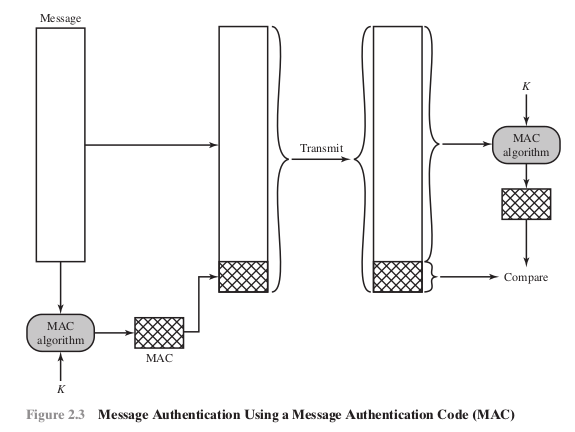
\includegraphics[width=14cm, keepaspectratio]{Bistarelli/img/cap_2/figura2.3.png}
\end{figure}

\paragraph{Funzione di hash a una via} Un'alternativa al codice di autenticazione dei messaggi è la funzione hash unidirezionale. Come nel caso del codice di autenticazione dei messaggi, una funzione di hash accetta in ingresso un messaggio M di dimensioni variabili e produce in uscita un digest del messaggio H(M) di dimensioni fisse (vedere Figura 2.4). In genere, il messaggio viene imbottito fino a un multiplo intero di una certa lunghezza fissa (ad esempio, 1024 bit) e l'imbottitura include il valore della lunghezza del messaggio originale in bit. Il campo della lunghezza è una misura di sicurezza per di sicurezza per aumentare la difficoltà per un aggressore di produrre un messaggio alternativo con lo stesso valore di hash.

\singlespacing

A differenza del MAC, una funzione di hash non riceve in ingresso una chiave segreta. La Figura 2.5 illustra tre modi in cui il messaggio può essere autenticato utilizzando una funzione hash.
Il digest del messaggio può essere crittografato utilizzando la crittografia simmetrica (vedere Figura 2.5a); se si presume che solo il mittente e il destinatario condividano la chiave di crittografia, l'autenticità è garantita.
Il message digest può anche essere crittografato con la crittografia a chiave pubblica (cfr. Figura 2.5b), come illustrato nella Sezione 2.3. L'approccio a chiave pubblica chiave pubblica presenta due vantaggi: 

\begin{enumerate}
    \item Fornisce una firma digitale
    
    \item L'autenticazione del messaggio e non richiede la distribuzione delle chiavi alle parti comunicanti
\end{enumerate}
Questi due approcci hanno un vantaggio rispetto a quelli che criptano l'intero messaggio, in quanto richiedono meno calcoli. Ma un approccio ancora più comune è l'uso di una tecnica che evita del tutto la crittografia. Diverse ragioni per questo interesse sono evidenziate in:

\begin{enumerate}
    \item \textbf{Il software di crittografia è piuttosto lento.}
    
    Anche se la quantità di dati da crittografia per ogni messaggio è piccola, può esserci un flusso costante di messaggi in entrata e in uscita da un sistema.

    \item \textbf{I costi dell'hardware di crittografia non sono trascurabili.} 
    
    Sono disponibili implementazioni su chip a basso costo di DES e AES, ma il costo aumenta se tutti i nodi di una rete devono avere questa capacità.
    
    \item \textbf{L'hardware di crittografia è ottimizzato per le grandi dimensioni dei dati.}
    
    Per piccoli blocchi di dati, un'alta percentuale del tempo viene spesa per l'overhead di inizializzazione/invocazione.
    
    \item \textbf{Un algoritmo di crittografia può essere protetto da un brevetto.}
\end{enumerate}

\begin{figure}[H]
	\centering
    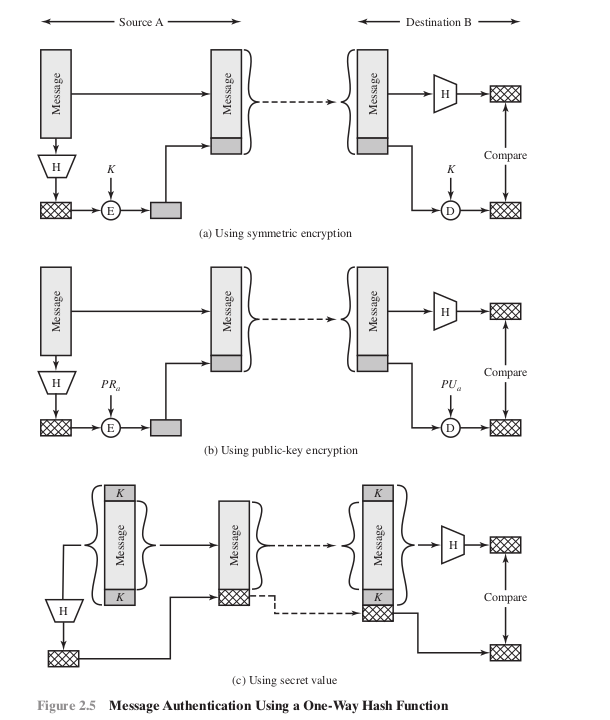
\includegraphics[width=14cm, keepaspectratio]{Bistarelli/img/cap_2/figura2.5.png}
\end{figure}


La Figura 2.5c mostra una tecnica che utilizza una funzione hash ma non la crittografia per l'autenticazione dei messaggi. Questa tecnica, nota come MAC hash a chiave, presuppone che due parti comunicanti, ad esempio A e B, condividano una chiave segreta comune K. Questa chiave segreta viene incorporata nel processo di generazione di un codice hash. Nell'approccio illustrato nella Figura 2.5c, quando A ha un messaggio da inviare a B, calcola la funzione di hash sulla concatenazione della chiave segreta e del messaggio: $M_{DM} = H(K || M || K)$. Quindi invia $[M  MD_{M}]$ a B. Poiché B possiede K, può ricalcolare $H(K ||  M ||  K)$ e verificare MDM. Dato che la chiave segreta non viene inviata, non dovrebbe essere possibile per un attaccante un aggressore di modificare un messaggio intercettato. Finché la chiave segreta rimane segreta, non dovrebbe essere possibile per un aggressore generare un messaggio falso.
Si noti che la chiave segreta viene utilizzata sia come prefisso che come suffisso del messaggio. Se la chiave segreta è usata solo come prefisso o solo come suffisso, lo schema è meno sicuro.

\newpage
\subsection{Altre applicazioni delle funzioni hash}
Ecco altri due esempi di applicazioni sicure delle funzioni hash:

\begin{itemize}
    \item \textbf{Password}
    
    In parole povere, quando un utente inserisce una password, l'hash di tale password viene confrontato con il valore di hash memorizzato per la verifica. Questa applicazione richiede resistenza alla preimmagine e forse una seconda resistenza alla preimmagine.
    
    \item \textbf{Rilevamento delle intrusioni}
    
    Memorizzare il valore di hash di un file, H(F), per ogni file su un sistema e proteggere i valori di hash (H(F)).
    Un sistema e proteggere i valori di hash (ad esempio, su un'unità bloccata in scrittura o su un disco ottico disco ottico write-once che viene tenuto al sicuro). È possibile determinare in seguito se un file è stato modificato calcolando nuovamente H(F). Un intruso dovrebbe modificare F senza modificare H(F).
\end{itemize}

\section{Crittografia a chiave pubblica}
\subsection{Struttura della crittografia a chiave pubblica}
Gli algoritmi a chiave pubblica sono basati su funzioni matematiche piuttosto che su semplici operazioni su schemi di bit, come quelle utilizzate negli algoritmi di crittografia simmetrica.  Inoltre, la crittografia a chiave pubblica è asimmetrica e prevede l'uso di due chiavi separate, a differenza della crittografia simmetrica che utilizza una sola chiave.

\singlespacing

L'uso di due chiavi ha profonde conseguenze nelle aree della riservatezza, della distribuzione delle chiavi e dell'autenticazione.

\singlespacing

Prima di procedere, è necessario menzionare alcune idee sbagliate comuni sulla crittografia a chiave pubblica. Una di queste è che la crittografia a chiave pubblica sia più sicura rispetto alla crittografia simmetrica. 
\singlespacing

In realtà, la sicurezza di qualsiasi schema di crittografia dipende da.

\begin{enumerate}

    \item \textbf{La lunghezza della chiave }
    
    \item \textbf{il lavoro computazionale necessario per di calcolo necessario per decifrare un cifrario}
\end{enumerate}

In linea di principio non c'è nulla nella crittografia simmetrica o della crittografia a chiave pubblica che ne renda una superiore all'altra dal punto di vista di resistenza agli attacchi. Una seconda convinzione errata è che la crittografia a chiave pubblica sia una tecnica di uso generale che ha reso obsoleta la crittografia simmetrica. Al contrario, a causa dell'overhead computazionale degli attuali schemi, non sembra che la crittografia simmetrica venga abbandonata.
Infine, si ha l'impressione che la distribuzione delle chiavi sia banale quando si usa la crittografia a chiave pubblica, rispetto a quella a chiave simmetrica. Per la distribuzione delle chiavi a chiave pubblica, è necessaria una qualche forma di protocollo, che spesso coinvolge un agente centrale, e le procedure non sono più semplici o più efficienti di quelle richieste per la crittografia simmetrica.

\singlespacing

Uno schema di crittografia a chiave pubblica ha sei ingredienti (vedi Figura 2.6a):

\begin{itemize}
    \item \textbf{Testo in chiaro}
    
    Si tratta del messaggio o dei dati leggibili che vengono inseriti nell'algoritmo come input.
    
    \item \textbf{Algoritmo di crittografia}
    
    L'algoritmo di crittografia esegue varie trasformazioni sul testo in chiaro.
    
    \item \textbf{Chiave Pubblica e Privata}
    
    Si tratta di una coppia di chiavi selezionate in modo che se una viene usata per la crittografia, l'altra viene usata per la decrittografia. Le trasformazioni esatte eseguite dall'algoritmo di crittografia dipendono dalla chiave pubblica o privata fornita in ingresso.
    
    \item \textbf{Testo cifrato}
    
    È il messaggio criptato prodotto in uscita. Dipende dal testo in chiaro e dalla chiave. Per un dato messaggio, due chiavi diverse produrranno due cifrari diversi.
    
    \item \textbf{Algoritmo di decrittazione}
    
    Questo algoritmo accetta il testo in chiaro e la chiave corrispondente e produce il testo in chiaro originale. 
\end{itemize}

Come suggeriscono i nomi, la chiave pubblica della coppia è resa pubblica e può essere utilizzata da altri, mentre la chiave privata è nota solo al suo proprietario. Un algoritmo crittografico di uso generale si basa su una chiave per la crittografia e su una chiave diversa ma correlata per la per la decifrazione.

\singlespacing

Le fasi essenziali sono le seguenti:

\begin{enumerate}

    \item Ogni utente genera una coppia di chiavi da utilizzare per la crittografia e la decrittografia dei messaggi.
    
    \item Ogni utente inserisce una delle due chiavi in un registro pubblico o in un altro file accessibile.
    
    \item Se Bob desidera inviare un messaggio privato ad Alice, Bob cripta il messaggio utilizzando la chiave pubblica di Alice.
    
    \item Quando Alice riceve il messaggio, lo decifra utilizzando la sua chiave privata. Nessun altro può decifrare il messaggio perché solo Alice conosce la chiave privata di Alice.
    
\end{enumerate}

\begin{figure}[H]
	\centering
    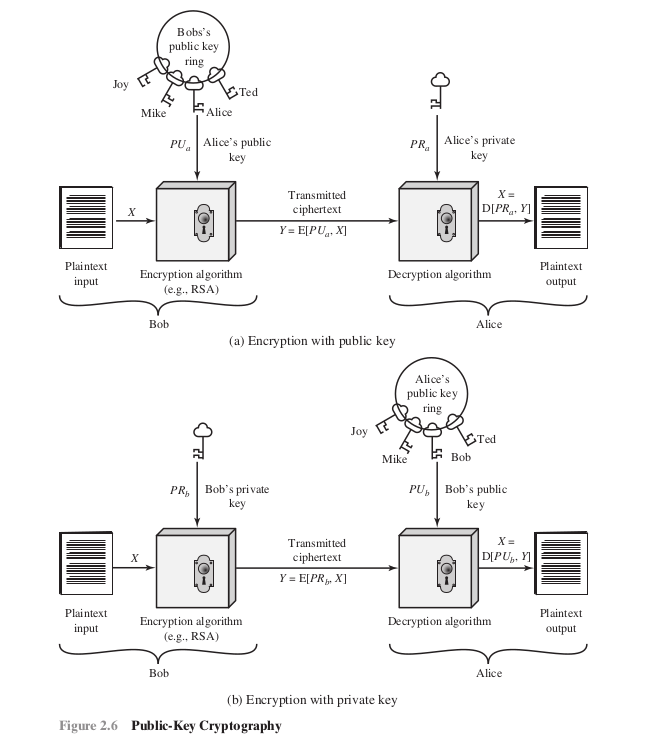
\includegraphics[width=14cm, keepaspectratio]{Bistarelli/img/cap_2/figura2.6.png}
\end{figure}

Con questo approccio, tutti i partecipanti hanno accesso alle chiavi pubbliche, mentre le chiavi private sono generate localmente da ogni partecipante e quindi non devono mai essere distribuite. Finché un utente protegge la propria chiave privata, la comunicazione in entrata è sicura. In qualsiasi momento, un utente può cambiare la chiave privata e pubblicare la nuova chiave pubblica che sostituisce la vecchia chiave pubblica.

\singlespacing

In questo schema, un utente cripta i dati utilizzando la propria chiave privata. Chiunque conosca la corrispondente chiave pubblica sarà in grado di decifrare il messaggio. Lo schema della Figura 2.6a è finalizzato a garantire la riservatezza. Solo il destinatario previsto deve essere in grado di decifrare il testo cifrato perché solo il destinatario previsto è in possesso di una chiave privata richiesta. 

\singlespacing

Lo schema della Figura 2.6b è finalizzato a fornire l'autenticazione e/o l'integrità dei dati. Se un utente è in grado di recuperare il testo in chiaro dal testo cifrato di Bob utilizzando la chiave pubblica di Bob, ciò indica che solo Bob può aver cifrato il testo in chiaro, fornendo così l'autenticazione. Inoltre, solo Bob sarebbe in grado di modificare il testo in chiaro perché solo Bob può cifrare il testo in chiaro con la chiave privata di Bob. 

\subsection{Applicazioni dei sistemi crittografici a chiave pubblica}
I sistemi a chiave pubblica sono caratterizzati dall'uso di un algoritmo di tipo crittografico con due chiavi, una privata e una pubblica. A seconda dell'applicazione, il mittente utilizza la chiave privata del mittente o la chiave pubblica del destinatario, o entrambe, per eseguire un tipo di funzione crittografica. In termini generali, possiamo classificare l'uso dei sistemi crittografici a chiave pubblica in tre categorie: firma digitale, distribuzione di chiavi simmetriche e crittografia di chiavi segrete.

\newpage
\subsection{Requisiti per la crittografia a chiave pubblica}
Il sistema crittografico illustrato nella Figura 2.6 dipende da un algoritmo crittografico
basato su due chiavi correlate. Diffie e Hellman hanno postulato questo sistema senza dimostrare l'esistenza di tali algoritmi.

\singlespacing

Tuttavia, hanno definito le condizioni che tali algoritmi devono soddisfare:

\begin{enumerate}
    \item È computazionalmente facile per una parte B generare una coppia (chiave pubblica $PU_b$, chiave privata $PR_b$).
    
    \item È computazionalmente facile per un mittente A, conoscendo la chiave pubblica e il messaggio da crittografare, M, per generare il corrispondente testo cifrato:
    
    \begin{center}
         $C = E(PU_b, M)$
    \end{center}
    
    \item È computazionalmente facile per il destinatario B decrittare il testo cifrato risultante utilizzando la chiave privata per recuperare il messaggio originale:
    
    \begin{center}
        $M = D(PR_b, C) = D[PR_b, E(PU_b, M)]$
    \end{center}
    
    \item È computazionalmente impossibile per un avversario, conoscendo la chiave pubblica, PUb, determinare la chiave privata, $PR_b$.
    
    \item  È computazionalmente impossibile per un avversario, conoscendo la chiave pubblica, PUb, e un testo cifrato, C, per recuperare il messaggio originale, M. Possiamo aggiungere un sesto requisito che, sebbene utile, non è necessario per tutte le applicazioni a chiave pubblica.
    
    \item Una delle due chiavi correlate può essere utilizzata per la crittografia e l'altra per la decrittografia.
    
    \begin{center}
        $M = D[PU_b, E(PR_b, M)] = D[PR_b, E(PU_b, M)]$
    \end{center}
\end{enumerate}

\begin{figure}[H]
	\centering
    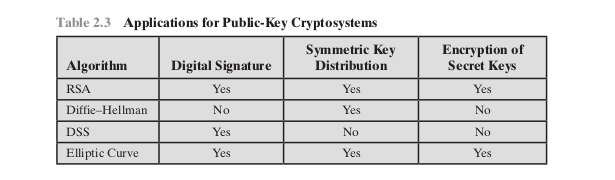
\includegraphics[width=14cm, keepaspectratio]{Bistarelli/img/cap_2/tabella2.3.png}
\end{figure}

\newpage
\subsection{Algoritmi di crittografia asimmetrica}
\paragraph{RSA} Lo schema RSA da allora regna sovrano come l'approccio alla crittografia a chiave pubblica. RSA è un cifrario a blocchi in cui il plaintext e il testo in chiaro e il testo cifrato sono numeri interi compresi tra 0 e $n - 1$ per qualche n. Per l'uso di RSA, è necessario utilizzare chiavi di dimensioni maggiori. Attualmente, una chiave di 1024 bit (circa 300 cifre decimali) è considerata abbastanza forte per quasi tutte le applicazioni.

\singlespacing

\paragraph{Accordo di chiave Diffie-Hellman} Il primo algoritmo a chiave pubblica pubblicato è apparso nell'articolo di Diffie e Hellman che ha definito la crittografia a chiave pubblica e viene generalmente chiamato scambio di chiavi Diffie-Hellman, o accordo di chiavi. Numerosi prodotti commerciali utilizzano questa tecnica di scambio di chiavi. Lo scopo dell'algoritmo è quello di permettere a due utenti di raggiungere in modo sicuro un accordo su un segreto condiviso che può essere usato come chiave segreta per la successiva crittografia simmetrica dei messaggi. L'algoritmo stesso si limita allo scambio delle chiavi.

\singlespacing


\paragraph{Standard di firma digitale} L'Istituto nazionale per gli standard e la tecnologia (NIST) ha pubblicato questo algoritmo come FIPS PUB 186 (Digital Signature Standard (DSS)). Il DSS fa uso di SHA-1 e presenta una nuova tecnica di firma digitale, l'algoritmo di firma digitale (DSA).  Il DSS utilizza un algoritmo progettato per fornire solo i dati di accesso al sistema. A differenza dell'RSA, non può essere utilizzato per la crittografia o lo scambio di chiavi.

\singlespacing

\paragraph{Crittografia a curva ellittica} La stragrande maggioranza dei prodotti e degli standard che utilizzano la crittografia a chiave pubblica per la crittografia e la firma digitale utilizzano RSA. La lunghezza dei bit per l'utilizzo sicuro di RSA è aumentata negli ultimi anni e ciò ha comportato un carico di elaborazione più pesante.
Questo ha comportato un carico di elaborazione maggiore per le applicazioni che utilizzano RSA. Recentemente, un sistema concorrente ha iniziato a sfidare RSA: la crittografia a curve ellittiche (ECC). L'ECC è già presente nelle iniziative di standardizzazione, tra cui l'IEEE (Istituto Elettrico). L'attrattiva principale dell'ECC rispetto all'RSA è che sembra offrire la stessa sicurezza per una dimensione di bit molto più piccola riducendo così l'overhead di elaborazione. D'altra parte, sebbene la teoria dell'ECC esista da tempo, è solo di recente che hanno cominciato ad apparire dei prodotti e che c'è stato un interesse crittoanalitico per la ricerca di punti deboli. Pertanto, il livello di fiducia nell'ECC non è ancora così alto come quello di RSA.
\newpage
\section{Firme digitali e gestione delle chiavi}
\subsection{Firme digitali}
La crittografia a chiave pubblica può essere utilizzata per l'autenticazione con una tecnica nota come firma digitale. Digital Signature Standard (DSS), definiscono la firma digitale come segue: Il risultato di una trasformazione crittografica di dati che, se correttamente implementata, fornisce un meccanismo per la verifica dell'origine l'autenticazione, l'integrità dei dati e il non ripudio del firmatario. Pertanto, una firma digitale è un modello di bit dipendente dai dati, generato da un agente in funzione di un file, di un messaggio o di un'altra forma di blocco di dati. 

\singlespacing

Il FIPS 186-4 specifica l'uso di uno dei tre algoritmi di firma digitale:
\begin{itemize}
    \item Algoritmo di firma digitale (DSA): L'algoritmo originale approvato dal NIST, che si basa sulla difficoltà di calcolo dei logaritmi discreti.
    
    \item Algoritmo di firma digitale RSA: Basato sull'algoritmo a chiave pubblica RSA.
    
    \item Algoritmo di firma digitale a curva ellittica (ECDSA): basato sulla crittografia a curva ellittica.
\end{itemize}

\begin{figure}[H]
	\centering
    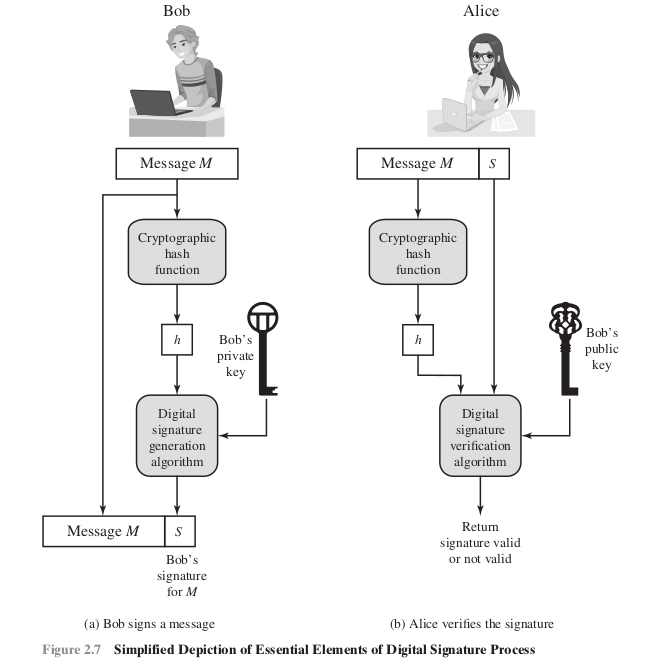
\includegraphics[width=14cm, keepaspectratio]{Bistarelli/img/cap_2/figura2.7.png}
\end{figure}


La Figura 2.7 è un modello generico del processo di creazione e utilizzo delle firme digitali. Tutti gli schemi di firma digitale previsti dal FIPS 186-4 hanno questa struttura. Supponiamo che Bob voglia inviare un messaggio ad Alice. Sebbene non sia importante che il messaggio segreto, Bob vuole che Alice abbia la certezza che il messaggio provenga da lui. A tal fine, Bob utilizza una funzione di hash sicura, come SHA-512, per generare un valore di hash per il messaggio. Questo valore di hash, insieme alla chiave privata di Bob, serve come input per un algoritmo di generazione della firma digitale che produce un breve blocco che funge da firma digitale. Bob invia il messaggio con la firma allegata.

\singlespacing

Quando Alice riceve il messaggio e la firma:

\begin{enumerate}
    \item calcola un valore di hash per il messaggio
    
    \item fornisce il valore di hash per il messaggio e la chiave pubblica di Bob come input a un algoritmo di verifica della firma digitale.
\end{enumerate}

Se l'algoritmo restituisce il risultato che la firma è valida, Alice ha la certezza che il messaggio è stato firmato da Bob. Nessun altro possiede la chiave privata di Bob e quindi nessun altro può aver creato una firma che possa essere verificata per questo messaggio con la chiave pubblica di Bob. Inoltre, è impossibile alterare il messaggio senza accedere alla chiave privata di Bob, quindi il messaggio è autenticato sia in termini di origine che di integrità dei dati. La firma digitale non garantisce la riservatezza. Cioè, il messaggio inviato  è al sicuro da alterazioni, ma non da intercettazioni. Questo è evidente nel caso di una firma basata su una parte del messaggio, perché il resto del messaggio viene trasmesso in chiaro. Anche nel caso di una crittografia completa, non c'è alcuna protezione della riservatezza, perché qualsiasi osservatore può decifrare il messaggio utilizzando la chiave pubblica del mittente. 

\subsection{Certificati a chiave pubblica}
Esiste un algoritmo a chiave pubblica ampiamente accettato, come RSA, ogni partecipante può inviare la propria chiave pubblica a qualsiasi altro partecipante o trasmettere la chiave alla comunità in generale. Sebbene questo approccio sia conveniente, ha una grande debolezza. Chiunque può falsificare tale annuncio pubblico. Cioè, un utente potrebbe fingere di essere Bob e inviare una chiave pubblica a un altro partecipante o trasmettere tale chiave pubblica. Finché Bob non scopre la falsificazione e avvisa gli altri partecipanti, il falsario è in grado di leggere tutti i messaggi cifrati destinati a Bob e può utilizzare le chiavi falsificate per l'autenticazione.

\singlespacing

\begin{figure}[H]
	\centering
    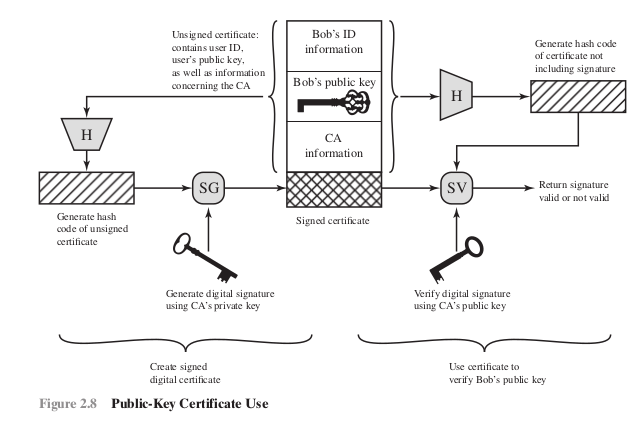
\includegraphics[width=14cm, keepaspectratio]{Bistarelli/img/cap_2/figura2.8.png}
\end{figure}

\textbf{La soluzione} a questo problema è il certificato a chiave pubblica. In sostanza, un certificato è costituito da una chiave pubblica più un ID utente del proprietario della chiave, con l'intero blocco firmato da una terza parte fidata. Il certificato include anche alcune informazioni sulla terza parte e un'indicazione del periodo di validità del certificato. In genere, la terza parte è un'autorità di certificazione (CA) di cui si fida la comunità degli utenti, come un'agenzia governativa o un'istituzione finanziaria. Un utente può presentare la propria chiave pubblica all'autorità in modo sicuro e ottenere un certificato firmato. L'utente può quindi pubblicare il certificato. Chiunque abbia bisogno della chiave pubblica di questo utente può ottenere il certificato e verificarne la validità attraverso la firma di fiducia allegata. La Figura 2.8 illustra il processo. Le fasi principali possono essere riassunte come segue:

\begin{enumerate}
    \item Il software utente (client) crea una coppia di chiavi: una pubblica e una privata.
    
    \item Il client prepara un certificato non firmato che include l'ID utente e la chiave pubblica dell'utente.
    
    \item L'utente fornisce il certificato non firmato a una CA in modo sicuro. Questo potrebbe un incontro faccia a faccia, l'uso di un'e-mail registrata o un modulo Web con verifica via e-mail.
    
    \item La CA crea una firma come segue:
        
        \begin{itemize}
            \item La CA utilizza una funzione hash per calcolare il codice hash del certificato non firmato.
            
            Una funzione di hash è una funzione che mappa un blocco di dati o un messaggio di lunghezza variabile in un valore di lunghezza fissa, chiamato codice hash.
            
            \item La CA genera la firma digitale utilizzando la chiave privata della CA e un algoritmo di generazione della firma.
            
        \end{itemize}
    
    \item La CA appone la firma al certificato non firmato per creare un certificato firmato.
    
    \item La CA restituisce al cliente il certificato firmato.
    
    \item Ogni utente può verificare la validità del certificato come segue:
        
        \begin{itemize}
            \item L'utente calcola il codice hash del certificato (esclusa la firma).
            
            \item L'utente verifica la firma digitale utilizzando la chiave pubblica della CA e l'algoritmo di verifica della firma. L'algoritmo restituisce un risultato di firma valida o non valida.
        \end{itemize}

\end{enumerate}
Uno schema è diventato universalmente accettato per la formattazione dei certificati a chiave pubblica, lo standard X.509. I certificati X.509 sono utilizzati nella maggior parte delle applicazioni per la sicurezza di rete, tra cui applicazioni di sicurezza di rete, tra cui IP Security (IPsec), Transport Layer Security (TLS), Secure Shell (SSH) e Secure Shell e Secure/Multipurpose Internet Mail Extension (S/MIME). La maggior parte di queste esamineremo la maggior parte di queste applicazioni nella quinta parte.

\subsection{Scambio di chiavi simmetriche con crittografia a chiave pubblica}
Con la crittografia simmetrica, un requisito fondamentale affinché due parti possano comunicare in modo sicuro è la condivisione di una chiave segreta. Supponiamo che Bob voglia creare un'applicazione di messaggistica che gli consenta di scambiare e-mail in modo sicuro con chiunque abbia accesso a Internet o a un'altra rete condivisa da entrambi. Supponiamo che Bob voglia farlo utilizzando la crittografia simmetrica. Con la crittografia simmetrica, Bob e la sua corrispondente, diciamo Alice, devono trovare un modo per condividere una chiave segreta unica che nessun altro conosce. Come possono farlo? Se Alice si trova nella stanza accanto a Bob, quest'ultimo potrebbe generare una chiave e scriverla su un foglio di carta o memorizzarla su un disco o una chiavetta e consegnarla ad Alice. Ma se Alice si trova dall'altra parte del continente o del mondo, cosa può fare Bob? Potrebbe criptare la chiave con la crittografia simmetrica e inviarla via e-mail ad Alice, ma ciò significa che Bob e Alice devono condividere una chiave segreta per criptare la nuova chiave segreta. Inoltre, Bob e chiunque altro utilizzi questo nuovo pacchetto di e-mail si trova ad affrontare lo stesso problema con ogni potenziale corrispondente: Ogni coppia di corrispondenti deve condividere una chiave segreta unica. Un approccio è l'uso dello scambio di chiavi Diffie-Hellman. Questo approccio è in effetti ampiamente utilizzato. Tuttavia, soffre dell'inconveniente che, nella sua forma più semplice, Diffie-Hellman non prevede l'autenticazione dei due interlocutori. Esistono esistono varianti di Diffie-Hellman che superano questo problema. Inoltre, esistono protocolli che utilizzano altri algoritmi a chiave pubblica che raggiungono lo stesso obiettivo.
\subsection{Buste Digitali}

\begin{figure}[H]
	\centering
    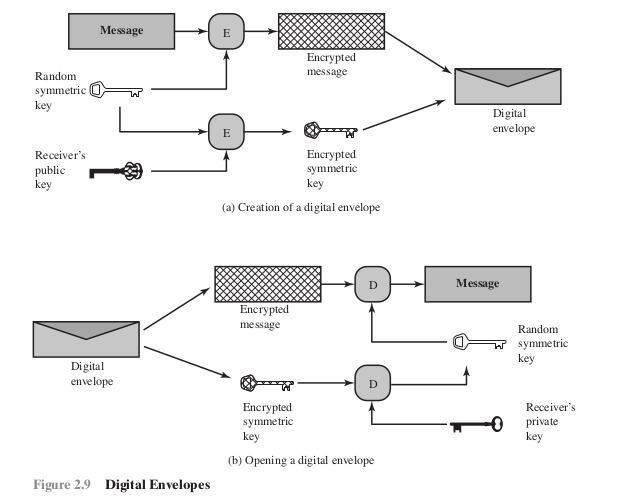
\includegraphics[width=14cm, keepaspectratio]{Bistarelli/img/cap_2/figura2.9.png}
\end{figure}


Un'altra applicazione in cui la crittografia a chiave pubblica viene utilizzata per proteggere una chiave simmetrica è la busta digitale, che può essere usata per proteggere un messaggio senza dover prima fare in modo che mittente e destinatario abbiano la stessa chiave segreta. La tecnica è denominata busta digitale, che è l'equivalente di una busta sigillata contenente una lettera non firmata. L'approccio generale è illustrato nella Figura 2.9. Supponiamo che Bob voglia inviare un messaggio riservato ad Alice, ma che non condivida una chiave segreta simmetrica. 

\singlespacing

Bob esegue le seguenti operazioni:

\begin{enumerate}

    \item Preparare un messaggio.
    
    \item Generare una chiave simmetrica casuale che verrà utilizzata una sola volta.
    
    \item Crittografare il messaggio utilizzando la crittografia simmetrica della chiave unica.
     
    \item Crittografare la chiave una tantum utilizzando la crittografia a chiave pubblica con la chiave pubblica di Alice.
    
    \item Allegare la chiave monouso crittografata al messaggio crittografato e inviarlo ad Alice.
    
\end{enumerate}
Solo Alice è in grado di decifrare la chiave a tempo unico e quindi di recuperare il messaggio originale. Se Bob ha ottenuto la chiave pubblica di Alice per mezzo del certificato di certificato a chiave pubblica di Alice, Bob ha la certezza che si tratta di una chiave valida.
\section{Applicazione pratica: Crittografia dei dati memorizzati}
Uno dei principali requisiti di sicurezza di un sistema informatico è la protezione dei dati memorizzati. I meccanismi di sicurezza per garantire tale protezione includono il controllo degli accessi, di rilevamento delle intrusioni e schemi di prevenzione delle intrusioni. Ma oltre agli approcci tecnici, questi approcci possono diventare vulnerabili a causa di fattori umani. Ne elenchiamo qui alcuni esempi, basati su:
\begin{itemize}
    \item Nel dicembre 2004, alcuni dipendenti della Bank of America hanno eseguito il backup e poi inviato al proprio centro dati di backup nastri contenenti i nomi dei clienti, gli indirizzi, i numeri di conto corrente e i numeri di previdenza sociale di 1,2 milioni di lavoratori pubblici iscritti a un conto con carta di credito. Nessuno dei dati era criptato. 
    
    I nastri non sono mai arrivati e non sono mai stati ritrovati. Purtroppo, questo metodo di backup e spedizione dei dati è fin troppo comune. Per fare un altro esempio, nell'aprile del 2005 Ameritrade ha incolpato il suo fornitore di spedizioni per aver perso un nastro di backup contenente informazioni non crittografate su 200.000 clienti.
    
    \item Nell'aprile del 2005, il San Jose Medical Group ha annunciato che qualcuno aveva fisicamente rubato uno dei suoi computer e un'altra parte di esso.
    
    \item Ci sono stati innumerevoli esempi di computer portatili persi negli aeroporti, rubati da una auto parcheggiata o presi mentre l'utente è lontano dalla sua scrivania. Se i dati sul disco non sono criptati, tutti i dati sono a disposizione del ladro.
\end{itemize}
Finché l'utente protegge la propria e non usa una password facilmente indovinabile, i file sono completamente protetti a protetti quando sono a riposo. 

\singlespacing

Alcuni approcci più recenti sono elencati in:

\begin{itemize}
    \item \textbf{Dispositivo back-end}
    
    Si tratta di un dispositivo hardware che si colloca tra i server e i sistemi di archiviazione e cripta tutti i file. Questi dispositivi criptano i dati a una velocità alla velocità del cavo, con una latenza molto ridotta. Al contrario, il software di crittografia sui server e sui sistemi di archiviazione rallenta i backup. 
    
    \item \textbf{Crittografia dei nastri basata su libreria}
    
    È fornita da una scheda co-processore incorporata nell'unità nastro e integrato nell'unità nastro e nell'hardware della libreria a nastro. Il co-processore cripta i dati utilizzando una chiave non leggibile configurata nella scheda. I nastri possono essere inviati fuori sede a una struttura che dispone dello stesso hardware dell'unità a nastro. La chiave può essere esportata tramite un' e-mail sicura o una piccola unità flash che viene trasportata in modo sicuro. 
    
    \item \textbf{Crittografia di base dei dati di laptop e PC}
    
    Diversi fornitori offrono prodotti prodotti software che forniscono una crittografia trasparente all'applicazione e all'utente. Alcuni prodotti crittografano tutti i file e le cartelle o una parte di essi. Altri prodotti, come altri prodotti, come BitLocker di Windows e FileVault di MacOS, crittografano un intero disco o un'immagine del disco o un'immagine del disco che si trova sul disco rigido dell'utente o su un dispositivo di archiviazione di rete.
\end{itemize}

    \newpage
\chapter*{Capitolo3}
\section{Principi dell'autenticazione digitale}
L'autenticazione dell'utente è la base per la maggior parte dei controlli di accesso e per la responsabilità dell'utente.
L'autenticazione dell'utente comprende due funzioni.

\begin{enumerate}
    \centering
    \item L'utente si identifica al sistema presentando una credenziale, come l'ID utente.
    \item Il sistema verifica l'utente attraverso lo scambio di informazioni di autenticazione.
\end{enumerate}

\paragraph{Esempio.} L'utente Alice Toklas potrebbe avere l'identificatore utente ABTOKLAS. Queste informazioni devono essere memorizzate su qualsiasi server o sistema di computer che Alice desidera utilizzare, e potrebbero essere note agli amministratori di sistema e ad altri utenti. Una tipica informazione di autenticazione associata a questo ID utente è una password, che è tenuta segreta (nota solo ad Alice e al sistema). Se nessuno è in grado di ottenere o indovinare la password di Alice, allora la combinazione di ID utente e password di Alice permette agli amministratori di impostare i permessi di accesso di Alice e di controllare la sua attività. Poiché l'ID di Alice non è segreto, gli utenti del sistema possono inviarle e-mail, ma poiché la sua password è segreta, nessuno può fingere di essere Alice.

\begin{itemize}
    \item \textbf{L'identificazione} è il mezzo con cui un utente fornisce un'identità dichiarata al sistema.
    \item \textbf{l'autenticazione} dell'utente è il mezzo per stabilire la validità della dichiarazione.
\end{itemize}

\paragraph{NIST SP 800-63-3 (Digital Authentication Guideline, ottobre 2016).}
Definisce l'autenticazione digitale degli utenti come il processo per stabilire la fiducia nelle identità degli utenti che sono presentate elettronicamente a un sistema informativo. I sistemi possono usare l'identità autenticata per determinare se l'individuo autenticato è autorizzato ad eseguire particolari funzioni, come le transazioni su database o l'accesso alle risorse del sistema. In molti casi, l'autenticazione e la transazione, o altre funzioni autorizzate, avvengono attraverso una rete aperta come Internet.

\newpage
\subsection{Un modello per l'autenticazione digitale degli utenti}
\paragraph{NIST SP 800-63-3} 
Definisce un modello generale per l'autenticazione dell'utente che coinvolge una serie di entità e procedure.
\\

Il requisito iniziale per eseguire l'autenticazione dell'utente è che l'utente deve essere registrato nel sistema. La seguente è una tipica sequenza per la registrazione. 

\begin{itemize}
    \item \textbf{Un richiedente} si rivolge a un'autorità di registrazione (RA) per diventare un abbonato di un fornitore di servizi di credenziali (CSP).
     \item \textbf{La RA} è un'entità fidata che stabilisce e garantisce l'identità di un richiedente a un CSP
     \item \textbf{Il CSP} poi si impegna in uno scambio con l'abbonato. A seconda dei dettagli del sistema di autenticazione globale, il CSP rilascia una sorta di credenziale elettronica al abbonato.
     \item \textbf{La credenziale} è una struttura di dati che lega autorevolmente un'identità e attributi aggiuntivi a un token posseduto da un abbonato, e può essere verificata quando viene presentata al verificatore in una transazione di autenticazione.
     \item \textbf{Il token} potrebbe essere una chiave di crittografia o una password criptata che identifica l'abbonato. Il token può essere emesso dal CSP, generato direttamente dall'abbonato o fornito da una terza parte.
\end{itemize}

Il token e la credenziale possono essere usati in successivi eventi di autenticazione.

\begin{figure}[H]
	\centering
    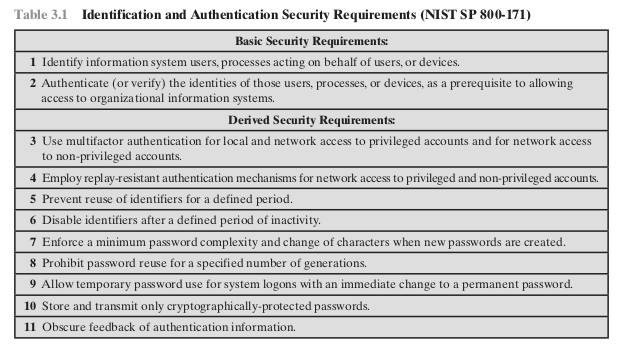
\includegraphics[width=14cm, keepaspectratio]{Bistarelli/img/cap_3/tabella3.1.png}
\end{figure}

\begin{figure}[H]
	\centering
    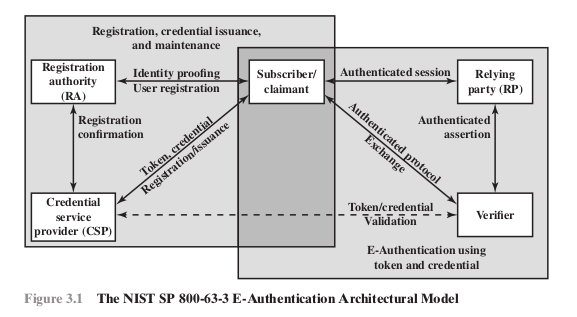
\includegraphics[width=14cm, keepaspectratio]{Bistarelli/img/cap_3/foto3.1.png}
\end{figure}

Una volta che un utente è registrato come abbonato, l'effettivo processo di autenticazione può avvenire tra l'abbonato e uno o più sistemi che eseguono l'autenticazione e, successivamente, l'autorizzazione. La parte che deve essere autenticata è chiamata richiedente e la parte che verifica tale identità è chiamata verificatore. Quando un richiedente dimostra con successo il possesso e il controllo di un token a un verificatore attraverso un protocollo di autenticazione, il verificatore può verificare che il richiedente sia il sottoscrittore indicato nella credenziale corrispondente. Il verificatore passa un'asserzione sull'identità del sottoscrittore alla parte fidata (RP).

\newpage
\subsection{Mezzi di Autenticazione}
Ci sono quattro mezzi generali per autenticare l'identità di un utente, che possono essere usati da soli o in combinazione:
\begin{enumerate}
    \item \textbf{Qualcosa che l'individuo conosce}
    
    Come una password, un numero di identificazione personale (PIN), o le risposte a una serie di domande prestabilite.
    
    \item \textbf{Qualcosa che l'individuo possiede}
    
    Come le keycard elettroniche, smart card e chiavi fisiche. Questo tipo di autenticatore è chiamato token.
    
    \item \textbf{Qualcosa che l'individuo è (biometria statica)}
    
    Come il riconoscimento per impronta digitale, retina e faccia.
    
    \item \textbf{Qualcosa che l'individuo fa (biometria dinamica)}
    
    Come il riconoscimento tramite il modello di voce, le caratteristiche della scrittura a mano e il ritmo di battitura.
\end{enumerate}
Tutti questi metodi, correttamente implementati e utilizzati, possono fornire un'autenticazione l'autenticazione dell'utente. Tuttavia, ogni metodo ha dei problemi. Un avversario può essere in grado di indovinare o rubare una password. Allo stesso modo, un avversario può essere in grado di falsificare o rubare un token. Un utente può dimenticare una password o perdere un token. 
\paragraph{L'autenticazione a più fattori} si riferisce all'uso di più di uno dei mezzi di autenticazione nella lista precedente. La forza dei sistemi di autenticazione è ampiamente determinata dal numero di fattori incorporati dal sistema. Le implementazioni che usano due fattori sono considerate più forti di quelle che usano un solo fattore. I sistemi che incorporano tre fattori sono più forti di quelli che ne incorporano solo due, e così via.

\newpage
\subsection{Valutazione dei rischi per l'autenticazione degli utenti}
Ci sono tre concetti separati che vogliamo mettere in relazione l'uno con l'altro: livello di sicurezza, impatto potenziale e aree di rischio.

\begin{itemize}
    \item \textbf{Livello di sicurezza}

Un livello di sicurezza descrive il grado di certezza di un'organizzazione che un utente ha presentato una credenziale che si riferisce alla sua identità. Più specificamente, la sicurezza è definita come:

    \item \textbf{Il grado di fiducia nel processo di controllo} utilizzato per stabilire l'identità dell'individuo a cui la credenziale è stata rilasciata.
    
    \item \textbf{Il grado di fiducia che l'individuo} che utilizza la credenziale sia l'individuo a cui la credenziale è stata rilasciata.
\end{itemize}
\paragraph{SP 800-63-3 riconosce quattro livelli di sicurezza:}
\begin{enumerate}
    \item \textbf{Livello:} poca o nessuna fiducia nella validità dell'identità asserita.
    
Un esempio in cui questo livello è appropriato è un consumatore che si registra per partecipare a una discussione sul sito web di un'azienda. La tipica tecnica di autenticazione a questo tipica a questo livello sarebbe un ID e una password forniti dall'utente al momento della transazione.
    
    \item \textbf{Livello:} una certa fiducia nella validità dell'identità asserita.

Le credenziali di livello 2 sono appropriate per un'ampia gamma di affari con il pubblico dove le organizzazioni che richiedono un'affermazione iniziale dell'identità (i cui dettagli sono verificati indipendentemente prima di qualsiasi azione). A questo livello, deve essere usato un qualche tipo di protocollo qualche tipo di protocollo di autenticazione sicura deve essere usato, insieme a uno dei mezzi di autenticazione riassunti in precedenza e discussi nelle sezioni successive.

    \item \textbf{Livello:} Alta fiducia nella validità dell'identità asserita
Questo livello è appropriato per permettere ai clienti o agli impiegati di accedere a servizi limitati di alto valore ma non al valore più alto.


    \item\textbf{Livello:} Fiducia molto alta nella validità dell'identità asserita
Questo livello è appropriato per permettere ai clienti o agli impiegati di accedere a servizi limitati di alto valore o per i quali un accesso improprio è molto dannoso.
\end{enumerate}

Un concetto strettamente legato a quello di livello di sicurezza è \textbf{il potenziale d'impatto}, definisce tre livelli di impatto potenziale sulle organizzazioni o sugli individui in caso di violazione della sicurezza (nel nostro contesto, un errore nell'autenticazione autenticazione dell'utente):

\begin{center}
    \textbf{Potenziale D'impatto}
\end{center}

\begin{itemize}
    \item \textbf{Low} Un errore di autenticazione potrebbe avere un effetto negativo limitato sulle operazioni organizzative, sulle risorse organizzative o sugli individui. Più specificamente, possiamo dire che l'errore potrebbe:
    
    \begin{itemize}
        \item Causare una degradazione della capacità capacità di missione in misura e durata tali che l'organizzazione sia in grado di eseguire le sue funzioni primarie, ma l'efficacia delle funzioni è notevolmente ridotta
        
        \item Provocare un danno minore ai beni dell'organizzazione
        
        \item Provocare una perdita finanziaria minore perdita finanziaria per l'organizzazione o gli individui
        
        \item Risultare in un danno minore agli individui.
    \end{itemize}
    
    \item \textbf{Moderate} Un errore di autenticazione potrebbe avere un serio effetto negativo effetto. Più specificamente, l'errore potrebbe:
    
    \begin{itemize}
        \item Causare una degradazione significativa nella capacità della missione in una misura e durata tale che l'organizzazione è in grado di eseguire le sue funzioni primarie, ma l'efficacia delle funzioni è significativamente.
        
        \item Provocare un danno significativo ai beni dell'organizzazione
        
        \item Provocare comporti una perdita finanziaria significativa
        
        \item Comporti un danno significativo alle persone che non che non implichi la perdita di vite umane o lesioni gravi in pericolo di vita.
    \end{itemize}
    \item \textbf{High}
    Un errore di autenticazione potrebbe avere un effetto negativo grave o catastrofico. L'errore potrebbe:
    \begin{itemize}
        \item Causare una grave degradazione o perdita della capacità della missione in misura e durata tali che l'organizzazione non sia in grado di eseguire una o più delle sue funzioni primarie
        
        \item Causare un grave danno ai beni dell'organizzazione
        
        \item Causare una grave perdita finanziaria all'organizzazione o agli individui
        
        \item Causare un danno grave o catastrofico agli individui che comporta la perdita della vita o lesioni gravi che mettono in pericolo la vita.
    \end{itemize}

\end{itemize}

La mappatura tra l'impatto potenziale e il livello appropriato di garanzia che è soddisfacente per affrontare l'impatto potenziale dipende dal contesto. La tabella 3.2 mostra una possibile mappatura per vari rischi a cui un'organizzazione può essere esposta. Questa tabella suggerisce una tecnica per fare la valutazione dei rischi. Per un dato sistema informativo o asset di servizio di un'organizzazione, l'organizzazione deve determinare il livello di impatto se si verifica un errore di autenticazione, usando le categorie di impatto, o aree di rischio, che sono preoccupanti. Per esempio, considerate il potenziale di perdita finanziaria se c'è un errore di autenticazione che risulta in un accesso non autorizzato a un database. A seconda della natura del del database, l'impatto potrebbe essere:

\begin{center}
    \textbf{Area di Rischio}
\end{center}

\begin{itemize}
    \item \textbf{Low} Nel peggiore dei casi, una perdita finanziaria insignificante o irrilevante perdita per qualsiasi parte, o nel peggiore dei casi, un'organizzazione insignificante o irrilevante responsabilità.
    
    \item \textbf{Moderate} Nel peggiore dei casi, una grave perdita finanziaria irrecuperabile per qualsiasi parte, o una grave responsabilità dell'organizzazione.

    
    \item \textbf{High} Grave o catastrofica perdita finanziaria irrecuperabile per qualsiasi parte; o grave o catastrofica responsabilità dell'organizzazione.
\end{itemize}
\newpage
\section{Autenticazione basata su password}

Una linea di difesa molto usata contro gli intrusi è il sistema di password. Praticamente tutti i sistemi multiutente, server basati sulla rete, siti di e-commerce basati sul web e altri servizi simili richiedono che un utente fornisca non solo un nome o un identificatore (ID) ma anche una password. Il sistema confronta la password con una password precedentemente memorizzata per quell'ID utente, conservata in un file di password di sistema. La password serve ad autenticare l'ID dell'individuo che accede al sistema. A sua volta, l'ID fornisce sicurezza nei seguenti modi:
\begin{itemize}
    \item \textbf{L'ID determina se l'utente è autorizzato ad accedere ad un sistema.}
    
    In alcuni sistemi, solo coloro che hanno già un ID depositato nel sistema sono permesso di accedere.
    
    \item \textbf{L'ID determina i privilegi accordati all'utente.}
    
    Alcuni utenti possono avere lo stato di amministratore o "superutente" che permette loro di leggere file ed eseguire funzioni che sono particolarmente protette dal sistema operativo. Alcuni sistemi hanno account ospiti o anonimi, e gli utenti di questi account hanno privilegi più privilegi più limitati degli altri.
    
    \item \textbf{L'ID è usato in quello che viene chiamato controllo di accesso discrezionale.}
    
    Per esempio esempio, elencando gli ID degli altri utenti, un utente può concedere loro il permesso di leggere i file di proprietà di quell'utente.
\end{itemize}
\newpage
\subsection{Vulnerabilità delle password}
\begin{itemize}
    \item \textbf{Attacco a dizionario offline:}
    
L'attaccante ottiene il file delle password di sistema e confronta gli hash delle password con gli hash delle password comunemente usate. Se viene trovata una corrispondenza, l'attaccante può ottenere l'accesso con quella combinazione ID/password.

        \begin{itemize}
            \item \textbf{Contromisure} 
            
            Includono controlli per prevenire l'accesso non autorizzato al file delle password, misure di rilevamento delle intrusioni per identificare una compromissione, e una rapida riemissione delle password se il file delle password viene compromesso.
        \end{itemize}

\item \textbf{Attacco all'account specifico}

L'attaccante prende di mira un account specifico e presenta password indovinate finché non viene scoperta la password corretta.

    \begin{itemize}
        \item \textbf{Contromisure} 
        
        è un meccanismo di blocco dell'account, che blocca l'accesso all'account dopo un certo numero di tentativi di accesso falliti. La pratica tipica è non più di di cinque tentativi di accesso.
    \end{itemize}

\item \textbf{Attacco con password popolare}

Una variante dell'attacco precedente consiste nell'utilizzare una password popolare e provarla contro una vasta gamma di ID utente. La tendenza di un utente è quella di scegliere una password che sia facilmente ricordabile; questo purtroppo rende la password facile da indovinare.

    \begin{itemize}
        \item \textbf{Contromisure} 
        
        Includono politiche per inibire la selezione da parte degli utenti di password comuni e la scansione degli indirizzi IP delle richieste di autenticazione e dei cookie del client per i modelli di invio.
    \end{itemize}

\item\textbf{Indovinare la password contro un singolo utente}

L'attaccante tenta di ottenere la conoscenza del titolare dell'account e delle politiche di password del sistema e usa tale conoscenza per indovinare la password.

    \begin{itemize}
        \item \textbf{Contromisure}
        
        Includono la formazione e l'applicazione di politiche sulle password che rendono le password difficili da indovinare.
    \end{itemize} 

\item\textbf{Dirottamento della stazione di lavoro}
L'attaccante aspetta fino a quando una stazione di lavoro loggata non è sorvegliata.

\begin{itemize}
    \item\textbf{Contromisure}
    
    è la registrazione automatica della workstation dopo un periodo di inattività. Gli schemi di rilevamento delle intrusioni possono essere usati per rilevare i cambiamenti nel comportamento dell'utente.
\end{itemize}

\item \textbf{Sfruttare gli errori dell'utente}

Se il sistema assegna una password, allora l'utente è più probabile che la scriva perché è difficile da ricordare. Questa situazione crea il potenziale per un avversario di leggere la password scritta. Un utente può condividere intenzionalmente una password, per permettere ad un collega di condividere i file, per esempio. Inoltre, gli aggressori hanno spesso successo nell'ottenere le password utilizzando tattiche di ingegneria sociale tattiche di ingegneria sociale che ingannano l'utente o un account manager a rivelare una password. Molti sistemi informatici sono forniti con password preconfigurate per gli amministratori di sistema. A meno che queste password preconfigurate non vengano cambiate, sono facilmente indovinate.

\begin{itemize}
    \item \textbf{Contromisure}
    
     la formazione degli utenti, il rilevamento delle intrusioni e password più semplici combinate con un altro meccanismo di autenticazione.
\end{itemize}

\item\textbf{Sfruttare l'uso di password multiple}

Gli attacchi possono anche diventare molto più efficaci o dannosi se diversi dispositivi di rete condividono la stessa password o una password simile per un dato utente. 

\begin{itemize}
    \item \textbf{Contromisure} 
    
    includono una politica che proibisce la stessa o password simili su particolari dispositivi di rete.
\end{itemize}
\newpage
\item \textbf{Monitoraggio elettronico}

Se una password viene comunicata attraverso una rete per accedere ad un sistema remoto, è vulnerabile alle intercettazioni. La semplice crittografia non risolve questo problema, perché la password criptata è, in effetti, la password e può essere osservata e riutilizzata da un avversario.
\end{itemize}
\subsection{Uso di password con hash}
Una tecnica di sicurezza delle password molto diffusa è l'uso di password con hash e di un valore di sale. Questo schema è presente in quasi tutte le varianti di UNIX e in numerosi altri sistemi operativi. Si utilizza la seguente procedura (vedi Figura 3.3). Per caricare una nuova password nel sistema, l'utente sceglie o gli viene assegnata una password. Questa password viene combinata con un valore di sale a lunghezza fissa. Nelle vecchie implementazioni, questo valore è legato al momento in cui la password è stata assegnata all'utente. 
\\
Le implementazioni più recenti utilizzano un numero pseudorandom o casuale. La password e il sale servono come input a un algoritmo di hashing per produrre un codice hash di lunghezza fissa.
\\
L'algoritmo di hash è progettato per essere lento nell'esecuzione al fine di contrastare gli attacchi. La password
hash viene memorizzata, insieme a una copia in chiaro del sale, nel file delle password dell'ID utente corrispondente.
file delle password per l'ID utente corrispondente. È stato dimostrato che il metodo della password hash è sicuro contro una serie di attacchi crittoanalitici.
\\
Quando un utente tenta di accedere a un sistema UNIX, fornisce un ID e una password (vedi Figura 3.1). e una password (vedi Figura 3.3b). Il sistema operativo utilizza l'ID per indicizzare il file delle password e recuperare "il sale" in chiaro e la password crittografata. "Il sale" e la password forniti dall'utente vengono utilizzati come input per la routine di crittografia. Se il risultato corrisponde al valore memorizzato, la password viene accettata.
\newpage
\paragraph{Il "sale" ha tre funzioni:}
\begin{enumerate}
    \item Impedisce che le password duplicate siano visibili nel file delle password. 
    
    Anche se due utenti scelgono la stessa password, a queste password saranno assegnati valori di valori di sale diversi. Di conseguenza, le password con hash dei due utenti saranno diverse.
    
    \item Questo aumenta notevolmente la difficoltà degli attacchi a dizionario offline. 
    
    Per un sale di lunghezza bits, il numero di password possibili aumenta di un fattore 2b, aumentando la difficoltà di indovinare una password la difficoltà di indovinare una password in un attacco a dizionario.
    
    \item Diventa quasi impossibile scoprire se una persona che ha password su due o più sistemi due o più sistemi abbia usato la stessa password su tutti.
    
\end{enumerate}

Per capire il secondo punto, considerate il modo in cui funzionerebbe un attacco a dizionario offline. L'attaccante ottiene una copia del file delle password. Supponiamo innanzitutto che il sale non venga utilizzato. L'obiettivo dell'attaccante è indovinare una singola password. A tal fine, l'attaccante sottopone alla funzione di hashing un gran numero di password probabili. Se una delle ipotesi corrisponde a uno degli hash del file, l'attaccante ha trovato una password che si trova nel file. Ma con lo schema UNIX, l'aggressore deve prendere ogni ipotesi e sottoporla alla funzione di hash una volta per ogni valore di sale nel file del dizionario, moltiplicando il numero di ipotesi da verificare. Lo schema di password UNIX è soggetto a due minacce. In primo luogo, un utente può ottenere l'accesso a una macchina utilizzando un account ospite o con altri mezzi e poi eseguire un programma per indovinare le password, chiamato password cracker, su quella macchina. L'attaccante dovrebbe essere in grado di controllare molte migliaia di possibili password con un consumo minimo di risorse. Inoltre, se l'avversario è in grado di ottenere una copia del file della password, il programma di cracking può essere eseguito a piacere su un altro computer. In questo modo, l'avversario può esaminare milioni di possibili password in un periodo di tempo ragionevole.

\begin{figure}[H]
	\centering
    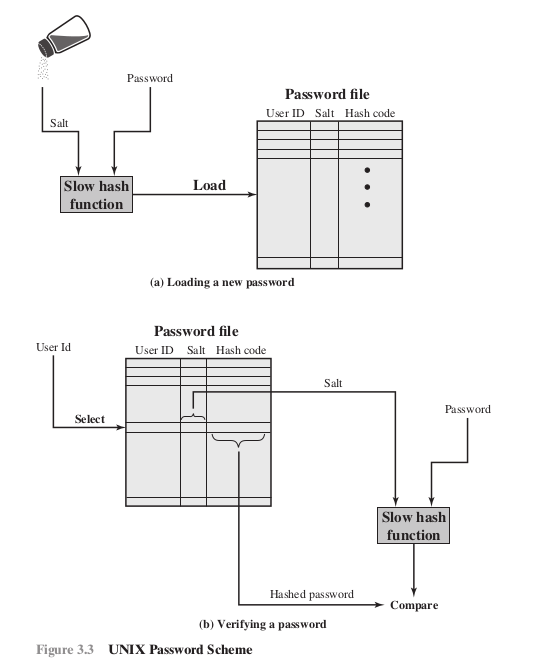
\includegraphics[width=14cm, keepaspectratio]{Bistarelli/img/cap_3/foto3.3.png}
\end{figure}
\newpage
\subsection{Cracking delle password scelte dall'utente}
\paragraph{Approccio Tradizionale}
L'approccio tradizionale all'indovinare le password, è quello di sviluppare un grande dizionario di possibili password e di provare ognuna di queste con il file delle password. Questo significa che ogni password deve essere sottoposta a un hash usando ogni valore di sale disponibile e poi confrontata con i valori di hash memorizzati. Se non viene trovata alcuna corrispondenza, il programma di cracking prova variazioni su tutte le parole del suo dizionario di password probabili. Tali variazioni includono l'ortografia a ritroso delle parole, numeri aggiuntivi o caratteri speciali, o sequenze di caratteri. Un'alternativa è quella di barattare lo spazio con il tempo precompilando i potenziali valori di hash. In questo approccio l'attaccante genera un grande dizionario di possibili password. Per ogni password, l'attaccante genera i valori di hash associati ad ogni possibile valore di sale. Il risultato è una mastodontica tabella di valori di hash nota come tabella arcobaleno.
\\
\paragraph{Approccio Moderno}
Purtroppo, questo tipo di vulnerabilità non è diminuita negli ultimi 25 anni o giù di lì. Gli utenti stanno facendo un lavoro migliore nel selezionare le password e le organizzazioni e le organizzazioni stanno facendo un lavoro migliore nel costringere gli utenti a scegliere password più forti, un concetto noto come politica delle password complesse. Tuttavia, le tecniche di cracking delle password sono migliorate per tenere il passo. I miglioramenti sono di due tipi. In primo luogo, la capacità di elaborazione disponibile per il cracking delle password è aumentata drammaticamente. Ora utilizzati sempre più per il calcolo, i processori grafici permettono ai programmi di cracking delle password di lavorare migliaia di volte più velocemente di quanto non facessero solo un dieci anni fa su PC di prezzo simile che usavano solo CPU tradizionali. Un PC che esegue una singola GPU AMD Radeon HD7970, per esempio, può provare in media una 8,2 * 109 combinazioni di password ogni secondo, a seconda dell'algoritmo utilizzato.
\singlespacing
La seconda area di miglioramento nel cracking delle password è l'uso di algoritmi sofisticati per generare potenziali password. I migliori risultati sono stati raggiunti studiando esempi di parole in uso. Per sviluppare tecniche che siano più efficienti ed efficaci dei semplici dizionario e degli attacchi brute-force, ricercatori e hacker hanno studiato la struttura struttura delle password. Per fare questo, gli analisti hanno bisogno di un grande pool di password di parole reali da studiare, cosa che ora hanno. La prima grande svolta è avvenuta alla fine del 2009, quando un attacco SQL injection contro il servizio di giochi online RockYou.com ha esposto 32 milioni di password in chiaro usate dai suoi membri per accedere ai loro account. Da da allora, numerosi set di file di password trapelate sono diventati disponibili per l'analisi.
\newpage
\subsection{Controllo dell'accesso ai file di password}
Un modo per contrastare un attacco con password è negare all'avversario l'accesso al file delle password. Se la porzione di password hash del file è accessibile solo da un utente privilegiato, allora l'avversario non può leggerla senza conoscere già la password di un utente privilegiato. Spesso, le password hash sono tenute in un file separato dagli ID utente, indicato come un file di password ombra.

Si presta particolare attenzione a rendere il file shadow password protetto da accessi non autorizzati. Anche se la protezione del file delle password sia certamente utile, rimangono delle vulnerabilità:

\begin{itemize}
    \item Molti sistemi, compresa la maggior parte dei sistemi UNIX, sono suscettibili di intrusioni.

Un hacker potrebbe essere in grado di sfruttare una vulnerabilità del software nel sistema operativo sistema operativo per bypassare il sistema di controllo degli accessi abbastanza a lungo da estrarre il file di password. In alternativa, l'hacker può trovare una debolezza nel file system o nel sistema di gestione del database che permette l'accesso al file.

    \item Un incidente di protezione potrebbe rendere il file delle password leggibile, rendendo così compromessi tutti gli account.

    \item Alcuni utenti hanno account su altre macchine in altri domini di protezione, e usano la stessa password. Quindi, se le password potrebbero essere lette da chiunque su una macchina, una macchina in un'altra posizione potrebbe essere compromessa.

    \item Una mancanza o una debolezza nella sicurezza fisica può fornire opportunità per un hacker.

A volte, c'è un backup del file delle password su un disco di riparazione disco di riparazione di emergenza o un disco di archiviazione. L'accesso a questo backup permette all'attaccante di leggere il file della password. In alternativa, un utente può avviare da un disco che esegue un altro sistema operativo come Linux e accedere al file da questo sistema operativo.


    \item Invece di catturare il file delle password di sistema, un altro approccio per raccogliere ID utente e password è attraverso lo sniffing del traffico di rete.
\end{itemize}
\singlespacing
Quindi, una politica di protezione delle password deve integrare le misure di controllo dell'accesso con tecniche per forzare gli utenti a scegliere password difficili da indovinare.
\newpage
\subsection{Strategie selezione password}
Quando non sono costretti, molti utenti scelgono una password troppo corta o troppo facile da indovinare. All'altro estremo, se agli utenti vengono assegnate password che consistono di otto caratteri stampabili scelti a caso, il cracking della password è effettivamente impossibile. Ma sarebbe quasi altrettanto impossibile per la maggior parte degli utenti ricordare le loro password. Il nostro obiettivo, quindi, è quello di eliminare le password indovinabili mentre permettendo all'utente di scegliere una password che sia memorizzabile. Quattro tecniche di base sono in uso:
\begin{enumerate}
    \item Educazione dell'utente
    \item Password generate dal computer
    \item Controllo reattivo delle password
    \item Politica delle password complesse
\end{enumerate}
\singlespacing
Gli utenti possono essere informati dell'importanza di usare password difficili da indovinare e possono essere fornire delle linee guida per la selezione di password forti. Questa strategia di educazione degli utenti è improbabile che abbia successo nella maggior parte delle installazioni, in particolare dove c'è una grande una vasta popolazione di utenti o molto turnover. Molti utenti semplicemente ignoreranno le linee guida. Altri possono non essere buoni giudici di ciò che è una password forte. Per esempio, molti utenti (erroneamente) credono che invertire una parola o scrivere in maiuscolo l'ultima lettera renda una password indovinabile
\newpage
\section{Autenticazione Basata sui token}
Gli oggetti che un utente possiede ai fini dell'autenticazione sono chiamati token.
\subsection{Memory Cards}
Le \textbf{Memory Cards} possono immagazzinare ma non elaborare dati.
\singlespacing
La più comune di queste carte è la carta bancaria con una banda magnetica sul retro. Una banda magnetica può memorizzare solo un semplice codice di sicurezza, che può essere letto (e sfortunatamente riprogrammato) da un economico lettore di carte. Ci sono anche schede di memoria che includono una memoria elettronica interna. Le carte di memoria possono essere usate da sole per
\begin{itemize}
    \item l'accesso fisico, come ad esempio in una stanza d'albergo.
    \item Per autenticazione, un utente fornisce sia la scheda di memoria che una qualche forma di password o numero di identificazione personale (PIN).
    
    Un'applicazione tipica è uno sportello automatico automatico (ATM). La scheda di memoria, se combinata con un PIN o una password, fornisce una sicurezza significativamente maggiore di una password da sola. Un avversario deve ottenere il possesso fisico possesso fisico della carta (o essere in grado di duplicarla) e in più deve ottenere la conoscenza del PIN. 
    \singlespacing
    Tra i potenziali inconvenienti NIST SP 800-12 (An Introduction to Computer Sicurezza: The NIST Handbook, ottobre 1995) nota quanto segue:
    \begin{itemize}
        \item \textbf{Richiede un lettore speciale}
        
        Questo aumenta il costo di utilizzo del token e crea l'obbligo di mantenere la sicurezza dell'hardware e del software del lettore.
        
        \item \textbf{Perdita dei token} 
        
        Un token perso impedisce temporaneamente al suo proprietario di ottenere l'accesso al sistema. Quindi, c'è un costo amministrativo nella sostituzione del token perso. Inoltre, se il token viene trovato, rubato o falsificato, allora un avversario deve solo determinare il PIN per ottenere un accesso non autorizzato.
        
        \item \textbf{Insoddisfazione dell'utente}
        
        Anche se gli utenti possono non avere difficoltà ad accettare l'uso di una scheda di memoria per l'accesso al bancomat, il suo uso per l'accesso al computer può essere considerato scomodo.
    \end{itemize}
\end{itemize}
\newpage
\subsection{Smart Cards}
Un'ampia varietà di dispositivi si qualificano come token intelligenti. Questi possono essere classificati lungo quattro dimensioni che non si escludono a vicenda:
\begin{itemize}
    \item \textbf{Caratteristiche fisiche} 
    
    I token intelligenti includono un microprocessore incorporato. Un token intelligente che assomiglia a una carta bancaria è chiamato smart card. Altri smart token possono assomigliare a calcolatrici, chiavi o altri piccoli oggetti portatili.
    
    \item \textbf{Interfaccia Utente}
    
    Le interfacce manuali includono una tastiera e un display per l'interazione uomo / interazione tra uomo e token.
     
    \item \textbf{Interfaccia Elettronica}
    
    Una smart card o un altro token richiede un'interfaccia elettronica elettronica per comunicare con un lettore/scrittore compatibile.
    
    \singlespacing
    
    Una carta può avere uno o entrambi i seguenti tipi di interfaccia:
    
    \begin{itemize}
        \item \textbf{Contatto}
        
        Una smart card a contatto deve essere inserita in un lettore di smart card con una connessione diretta a una piastra di contatto conduttiva sulla superficie della carta (tipicamente placcata in oro).
        
        La trasmissione di comandi, dati e stato della carta avviene attraverso questi punti di contatto fisico.

        \item \textbf{Senza Contatto}
        
        Una carta senza contatto richiede solo la vicinanza di un lettore.
        
        Sia il lettore che la carta hanno un'antenna, e i due comunicano utilizzando frequenze radio. La maggior parte delle carte senza contatto derivano anche l'energia per il chip interno da questo segnale elettromagnetico. La portata è tipicamente da un mezzo a tre pollici per le carte non alimentate a batteria, ideale per applicazioni come l'ingresso in un edificio e il pagamento che richiedono un'interfaccia della carta molto veloce.
        
        \item \textbf{Protocollo di autenticazione}
        
        Lo scopo di un token intelligente è quello di fornire un mezzo per l'autenticazione dell'utente.
        
        \newpage
        
        Possiamo classificare i protocolli di autenticazione usati con token intelligenti in tre categorie:
        
        \begin{enumerate}
            \item \textbf{Statico}
            
            Con un protocollo statico, l'utente si autentica con il token, poi il token autentica l'utente al computer. L'ultima metà di questo protocollo è simile al funzionamento di un token di memoria.
            
            \item \textbf{Generatore dinamico di password}
            
            In questo caso, il token genera una password unica password unica periodicamente (ad esempio, ogni minuto). Questa password viene poi inserita nel sistema informatico per l'autenticazione, sia manualmente dall'utente o elettronicamente tramite il token. Il token e il sistema informatico devono essere inizializzati e mantenuti sincronizzati in modo che il computer conosca la password che è corrente per questo token.
            
            \item \textbf{Sfida-risposta}
            
            In questo caso, il sistema informatico genera una sfida, come una stringa casuale di numeri. Il token intelligente genera una risposta basata sulla sfida. Per esempio, si potrebbe usare la crittografia a chiave pubblica e il token potrebbe criptare la stringa di sfida con la chiave privata del token.
        \end{enumerate}
    \end{itemize}
\end{itemize}
\newpage
\subsection{Elettronic Identity Cards}
Un'applicazione di crescente importanza è l'uso di una smart card come carta d'identità nazionale per i cittadini. Una carta d'identità elettronica nazionale (eID) può servire agli stessi scopi di altre carte d'identità nazionali, e carte simili come la patente di guida, per l'accesso ai servizi governativi e commerciali. Inoltre, una carta eID può fornire una prova di identità più forte ed essere usata in una più ampia varietà di applicazioni. In effetti, una carta eID è una smart card che è stata verificata dal governo nazionale come valida e autentica.
\singlespacing
L'identity cards conterrà:
\begin{itemize}
    \item Dati personali 
    
    Come nome, data di nascita e indirizzo
    
    \item Numero del documento
    
    Un identificatore alfanumerico di nove caratteri unico per ogni carta.

    \item Numero di accesso alla carta (CAN)
    
    Un numero decimale casuale di sei cifre stampato sulla faccia della carta.
    
    \item Zona a lettura ottica (MRZ)
    
     Tre righe di testo leggibile dall'uomo e dalla macchina sul retro della carta. Anche questo può essere usato come password.
\end{itemize}
Le funzioni dell'identiry cards sono:
\begin{itemize}
    \item \textbf{ePass}
    
    Questa funzione è riservata all'uso governativo e memorizza una rappresentazione digitale dell'identità del titolare della carta. Questa funzione è simile a, e può essere usata per, un passaporto elettronico. Anche altri servizi governativi possono usare ePass. La funzione ePass deve essere implementata sulla carta.
    
    \item \textbf{eID}
    
    Questa funzione è per uso generale in una varietà di applicazioni governative e commerciali. applicazioni commerciali. La funzione eID memorizza un record di identità a cui i servizi autorizzati possono accedere con il permesso del titolare della carta. I cittadini scelgono se vogliono attivare questa funzione.
    
    \item \textbf{eSign}
    
    Questa funzione opzionale memorizza una chiave privata e un certificato che verifica la chiave; è usata per generare una firma digitale. Un centro di fiducia del settore privato emette il certificato.
\end{itemize}
\section{Autenticazione Biometrica}
Un sistema di autenticazione biometrica tenta di autenticare un individuo sulla base di le sue caratteristiche fisiche uniche. Queste includono:
\begin{itemize}
    \item \textbf{Caratteristiche statiche}
    
    come le impronte digitali, la geometria della mano, le caratteristiche del viso e i modelli della retina e dell'iride
    
    \item \textbf{Caratteristiche dinamiche}
    
    come l'impronta vocale e la firma.
\end{itemize}
In sostanza, la biometria si basa sul riconoscimento dei modelli. Rispetto alle password e ai token, l'autenticazione è tecnicamente più complessa e costosa. Sebbene sia usata in un numero di applicazioni specifiche, la biometria deve ancora maturare come strumento standard per l'autenticazione degli utenti ai sistemi informatici.
\subsection{Caratteristiche fisiche utilizzate nelle applicazioni biometriche}
Un certo numero di diversi tipi di caratteristiche fisiche sono in uso o in fase di studio per l'autenticazione dell'utente. Le più comuni sono le seguenti:

\begin{itemize}
    \item \textbf{Caratteristiche facciali}
    
    Le caratteristiche facciali sono il mezzo più comune per l'identificazione da uomo a uomo; quindi è naturale considerarle per l'identificazione tramite computer. L'approccio più comune è quello di definire le caratteristiche basate sulla posizione relativa e la forma delle caratteristiche facciali chiave, come occhi, sopracciglia, naso, labbra e forma del mento.
    
    \item \textbf{Impronte digitali}
    
    Le impronte digitali sono state usate come mezzo di identificazione per secoli, e il processo è stato sistematizzato e automatizzato in particolare per l'applicazione della legge. Un'impronta digitale è il modello di creste e solchi sulla superficie del polpastrello. Si ritiene che le impronte digitali siano uniche in l'intera popolazione umana. In pratica, il riconoscimento automatico delle impronte digitali e sistema di corrispondenza estrae un certo numero di caratteristiche dall'impronta digitale per memorizzarle come surrogato numerico del modello completo dell'impronta digitale.
    
    \item \textbf{Geometria della mano}

    I sistemi di geometria della mano identificano le caratteristiche della mano, compresa la forma, la lunghezza e la larghezza delle dita.
    
    \item \textbf{Modello della retina}
    
    Il modello formato dalle vene sotto la superficie della retina è unico e quindi adatto all'identificazione. Un sistema biometrico retinico ottiene un'immagine digitale del modello retinico proiettando un fascio di luce visiva o infrarossa a bassa intensità nell'occhio.
    
    \item \textbf{Iride}
    
    Un'altra caratteristica fisica unica è la struttura dettagliata dell'iride.
    
    \item \textbf{Firma}
    
    Ogni individuo ha uno stile unico di scrittura e questo si riflette specialmente nella firma, che è tipicamente una sequenza scritta frequentemente. Tuttavia, più campioni di firma di un singolo individuo non saranno identici.
    
    \item \textbf{La voce}
    
    Mentre lo stile della firma di un individuo riflette non solo gli unici attributi fisici dello scrittore ma anche l'abitudine alla scrittura che si è sviluppata, i modelli di voce sono più strettamente legati alle caratteristiche fisiche e anatomiche del parlante. Ciononostante, c'è ancora una variazione da campione a campione nel tempo dallo stesso parlante, complicando il compito di riconoscimento biometrico.
\end{itemize}
\newpage
\subsection{Funzionamento di un sistema di autenticazione biometrica}
Ogni individuo che deve essere incluso nel database degli utenti autorizzati deve prima essere iscritto al sistema. Questo è analogo all'assegnazione di una password a un utente. Per un sistema biometrico, l'utente presenta al sistema un nome e, tipicamente, un qualche tipo di password o PIN. Allo stesso tempo, il sistema rileva alcune caratteristiche biometriche di questo utente (ad esempio, l'impronta digitale del dito indice destro). Il sistema digitalizza l'input e poi estrae un insieme di caratteristiche che possono essere memorizzate come un numero o un insieme di numeri che rappresentano questa caratteristica biometrica unica; questo insieme di numeri viene chiamato template dell'utente. L'utente è ora iscritto al sistema, che mantiene per l'utente un nome (ID), forse un PIN o una password, e il valore biometrico.
\singlespacing
A seconda dell'applicazione, l'autenticazione dell'utente su un sistema biometrico comporta la verifica o l'identificazione.
\begin{itemize}
    \item \textbf{Verifica}
    
    è analoga a quella di un utente che accede a un sistema usando una scheda di memoria o una smart card accoppiata a una password o a un PIN. Per la verifica biometrica, l'utente inserisce un PIN e utilizza anche un sensore biometrico. Il sistema estrae la caratteristica corrispondente e la confronta con il modello memorizzato per questo utente. Se c'è una corrispondenza, allora il sistema autentica questo utente.
    
    \item \textbf{Identificazione}
    
    l'individuo usa il sensore biometrico ma non presenta informazioni aggiuntive. Il sistema quindi confronta il modello presentato con l'insieme dei modelli memorizzati. Se c'è una corrispondenza, l'utente viene identificato. Altrimenti, l'utente viene rifiutato.
\end{itemize}

\begin{figure}[H]
	\centering
    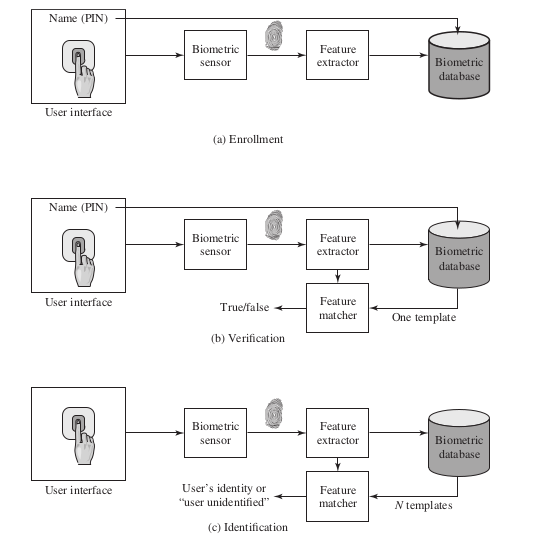
\includegraphics[width=14cm, keepaspectratio]{Bistarelli/img/cap_3/figura3.9.png}
\end{figure}

\begin{figure}[H]
	\centering
    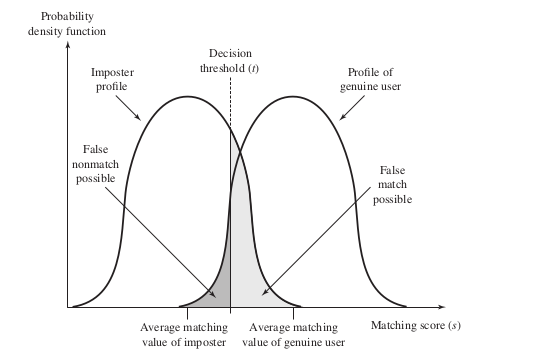
\includegraphics[width=14cm, keepaspectratio]{Bistarelli/img/cap_3/figura3.10.png}
\end{figure}
\subsection{Precisione Biometrica}
In qualsiasi schema biometrico, alcune caratteristiche fisiche dell'individuo sono mappate in una rappresentazione digitale. Per ogni individuo, una singola rappresentazione digitale, o template, è memorizzata nel computer. Quando l'utente deve essere autenticato, il sistema confronta il modello memorizzato con il modello presentato. Data la complessità delle caratteristiche fisiche, non ci si può aspettare che ci sia una corrispondenza esatta tra i due modelli. Piuttosto, il sistema usa un algoritmo per generare un punteggio (tipicamente un singolo numero) che quantifica la somiglianza tra l'input e il modello memorizzato. Per procedere con la discussione, definiamo i seguenti termini.
\begin{itemize}
    \item Il tasso di falsa corrispondenza
    
    è la frequenza con cui i campioni biometrici provenienti da diverse fonti diverse sono erroneamente valutati come provenienti dalla stessa fonte. Il tasso di falsa non corrispondenza è la frequenza con cui i campioni della stessa fonte sono erroneamente valutati essere di fonti diverse.
    
    \item La funzione di densità
    
    tipicamente forma una curva a campana.
\end{itemize}
\begin{figure}[H]
	\centering
    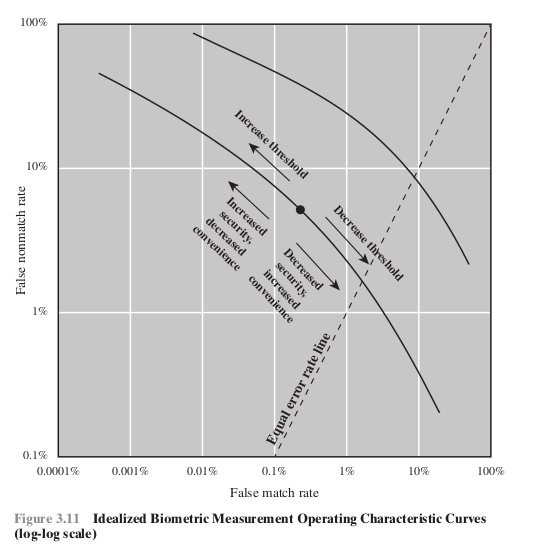
\includegraphics[width=14cm, keepaspectratio]{Bistarelli/img/cap_3/figura3.11.png}
\end{figure}
\singlespacing
\paragraph{Esempio} nel caso di un'impronta digitale, i risultati possono variare a causa del rumore del sensore, dei cambiamenti nell'impronta dovuti al gonfiore o alla secchezza, del posizionamento del dito e così via. In media, qualsiasi altro individuo dovrebbe avere un punteggio di corrispondenza molto più basso, ma ancora una volta mostrerà una funzione di densità di probabilità a campana. La difficoltà è che la gamma di punteggi di corrispondenza prodotti da due individui, uno autentico e uno impostore, rispetto a un dato modello di riferimento, è probabile che si sovrappongano. Nella figura 3.10, un valore di soglia è selezionato in modo che se il valore presentato s >= t si assume una corrispondenza, e per s < t, si assume una mancata corrispondenza. La parte ombreggiata a destra di t indica una gamma di valori per cui è possibile una falsa corrispondenza, e la parte ombreggiata a sinistra indica una gamma di valori per cui è possibile una falsa non corrispondenza. Una falsa corrispondenza comporta l'accettazione di un utente che non dovrebbe essere accettato, e una falsa mancata corrispondenza provoca il rifiuto di un utente valido. L'area di ogni parte ombreggiata rappresenta la probabilità di una falsa corrispondenza o non corrispondenza, rispettivamente. Spostando la soglia, a sinistra o a destra, le probabilità possono essere alterate, ma si noti che una diminuzione del tasso di falsi riscontri si traduce in un aumento del tasso di falsi non riscontri, e viceversa.
\section{Autenticazione Remota dell'utente}
La forma più semplice di autenticazione dell'utente è l'autenticazione locale, in cui un utente tenta di accedere a un sistema che è presente localmente, come un PC da ufficio stand-alone o un bancomat. Il caso più complesso è quello dell'autenticazione remota dell'utente, che avviene su Internet, una rete o un collegamento di comunicazione. L'autenticazione remota dell'utente solleva ulteriori minacce alla sicurezza, come un intercettatore in grado di catturare una password, o un avversario che riproduce una sequenza di autenticazione che è stata osservata.
\newpage
\subsection{Protocollo delle password}
In questo esempio, un utente trasmette prima la sua identità a all'host remoto. L'host genera un numero casuale r, spesso chiamato nonce, restituisce questo nonce all'utente.
\singlespacing
Inoltre, l'host specifica due funzioni, h() e f(), da utilizzare nella risposta. Questa trasmissione dall'host all'utente è la sfida. La risposta dell'utente è la quantità f(r', h(P')), dove r' = r e P' è la password dell'utente.
\singlespacing
La funzione h è una funzione hash, quindi la risposta consiste nella funzione hash della password dell'utente combinata con il numero casuale utilizzando la funzione.
\singlespacing
L'host memorizza la funzione hash della password di ogni utente registrato, rappresentata come h(P(U)) per l'utente U. Quando arriva la risposta, l'host confronta f(r', h(P')) con la f(r, h(P(U)) calcolata.) Se le quantità corrispondono, l'utente è autenticato. Questo schema difende da diverse forme di attacco. L'host memorizza non la password ma un codice hash della password. Questo protegge la password dagli intrusi nel sistema host. Inoltre, nemmeno l'hash della password viene trasmesso direttamente, ma piuttosto una funzione in cui l'hash della password è uno degli argomenti. Così, per una funzione f adatta, l'hash della password non può essere catturato durante la trasmissione.
\singlespacing
Infine, l'uso di un numero casuale tenta di difendere da un attacco di replay, in cui un avversario cattura la trasmissione dell'utente e tenta di accedere a un sistema ritrasmettendo i messaggi.
\begin{figure}[H]
	\centering
    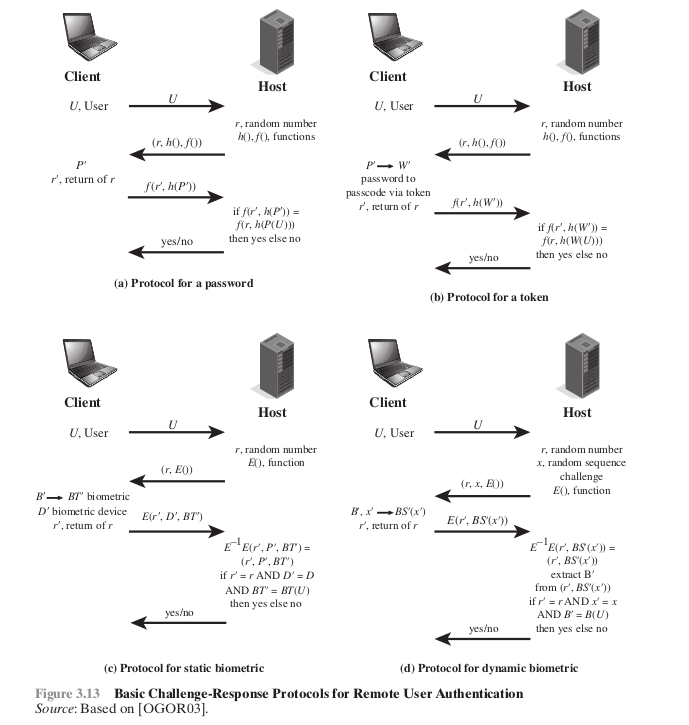
\includegraphics[width=14cm, keepaspectratio]{Bistarelli/img/cap_3/figura3.13.png}
\end{figure}
\subsection{Protocollo di Token}
Come prima, un utente trasmette prima la sua identità all'host remoto. L'host restituisce un numero casuale e gli identificatori delle funzioni f() e h() da utilizzare nella risposta. Alla fine dell'utente, il token fornisce un codice di accesso W'. Il token memorizza un codice statico statico o genera un codice casuale una tantum. Per un codice casuale una tantum, il token deve essere sincronizzato. Per un codice casuale una tantum, il token deve essere sincronizzato in qualche modo con l'host. In entrambi i casi, l'utente attiva il codice inserendo una password P'. Questa password è condivisa solo tra l'utente e il token e non coinvolge l'host remoto. Il token risponde all'host con la quantità f(r', h(W')). Per un codice di accesso statico, l host memorizza il valore hashed h(W(U)); per un passcode dinamico, l'host genera un passcode una tantum (sincronizzato con quello generato dal token) e prende il suo hash. L'autenticazione procede poi nello stesso modo del protocollo della password.
\subsection{Protocollo biometrico statico}
Come prima cosa, l'utente trasmette un ID all'host, che risponde con un numero casuale r e, in questo caso, l'identificatore di una crittografia E(). Sul lato utente c'è un sistema client che controlla un dispositivo biometrico. Il sistema genera un template biometrico BT' dal biometrico dell'utente B' e restituisce il testo cifrato E(r', D', BT'), dove D' identifica questo particolare dispositivo biometrico. L'host decifra il messaggio in arrivo per recuperare i tre parametri trasmessi e li confronta con i valori memorizzati localmente.
\singlespacing
Per una corrispondenza, l'host deve trovare r' = r. Inoltre, il punteggio di corrispondenza tra BT' e il modello memorizzato deve superare una soglia predefinita. Infine, l'host fornisce una semplice autenticazione del dispositivo di cattura biometrica confrontando l'ID del dispositivo in entrata con un elenco di dispositivi registrati nel database dell'host.
\subsection{Protocollo Biometrico Dinamico}
La principale differenza rispetto al caso di una biometria stabile è che l'host fornisce una sequenza casuale fornisce una sequenza casuale e un numero casuale come sfida. La sfida è una sequenza di numeri, caratteri o parole. L'utente umano all'estremità del client deve quindi vocalizzare (verifica con altoparlante), digitare (verifica dinamica della tastiera) o scrivere (verifica a mano) o scrivere (verifica della scrittura) la sequenza per generare un segnale biometrico BS'(x'). Il lato client cripta il segnale biometrico e il numero casuale. All'indirizzo lato host, il messaggio in arrivo viene decifrato. Il numero casuale in arrivo r' deve essere una corrispondenza esatta con il numero casuale che è stato originariamente utilizzato come sfida (r). Inoltre, l'host genera un confronto basato sul segnale biometrico in entrata biometrico BS'(x'), il template memorizzato BT(U) per questo utente e il segnale originale x. Se il valore di confronto supera una soglia predefinita, l'utente viene autenticato.
    \chapter{Keberos}
Imitologia Greca: cane a tre teste guardiano delle porte dell’ade. Sviluppato a fine anni ‘80, il goal: segretezza, autentica (ad accesso singolo), temporalità o Le chiavi usate hanno validità limitata onde prevenire replay attack. Usa i timespamp, che richiedono macchine sincronizzate, contro replay attack. 

\begin{figure}[H]
	\centering
    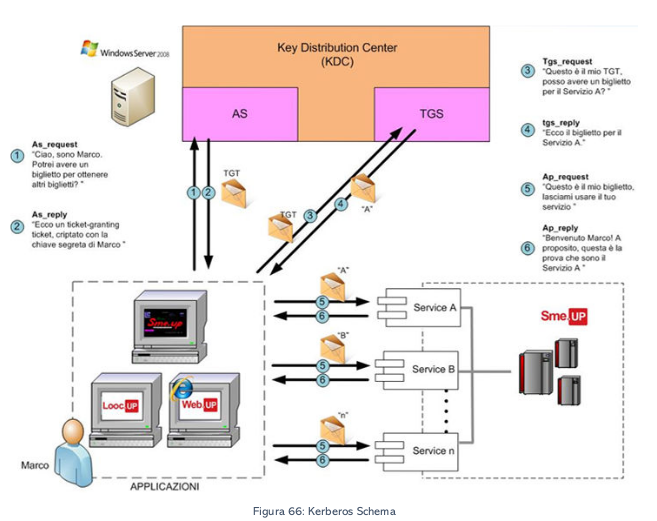
\includegraphics[width=7cm, keepaspectratio]{Bistarelli/img/keberos/keberos1.png}
\end{figure}

\begin{figure}[H]
	\centering
    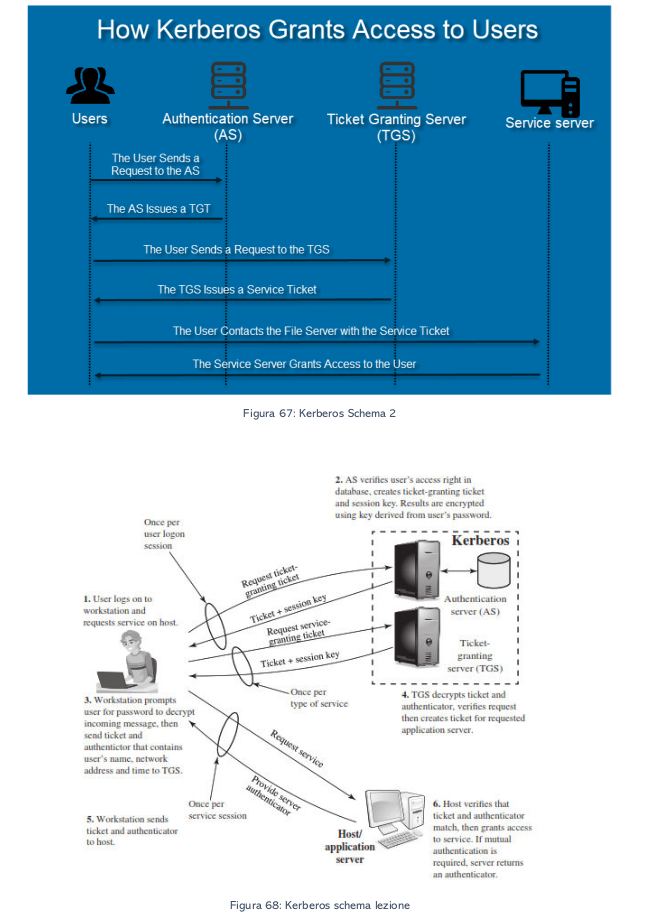
\includegraphics[width=7cm, keepaspectratio]{Bistarelli/img/keberos/keberos2.png}
\end{figure}

\subsection{Caratteristiche}
\begin{itemize}
    \item 3 fasi: autenticazione, autorizzazione, servizio
    
    \item Ultime 2 opzionali e trasparenti all’utente
    
    \item Ognuna fornisce credenziali per successiva
    
    \begin{itemize}
        \item Fase 1 fornische authKey e authTicket per la 2
        
        \item Fase 2 fornisce servKey e servTicket per la fase 3
    \end{itemize}
    
    \item Ogni tipo di chiave si sessione ha sua durata (in genere quelle per i servizi dura meno, es. sessione 1 giorno, servizio 1 ora)
    
    \item Una authKey può criptare divere servKey
    
\end{itemize}
\textbf{Nota:} Chiave pubblica e privata per autenticazione, chiave di sessione per la sessione (authKey e servKey)
perché ha una durata limitata e servono a dare confidentiality/confidenzialità a questa comunicazione in modo da
cifrarla.

\begin{figure}[H]
	\centering
    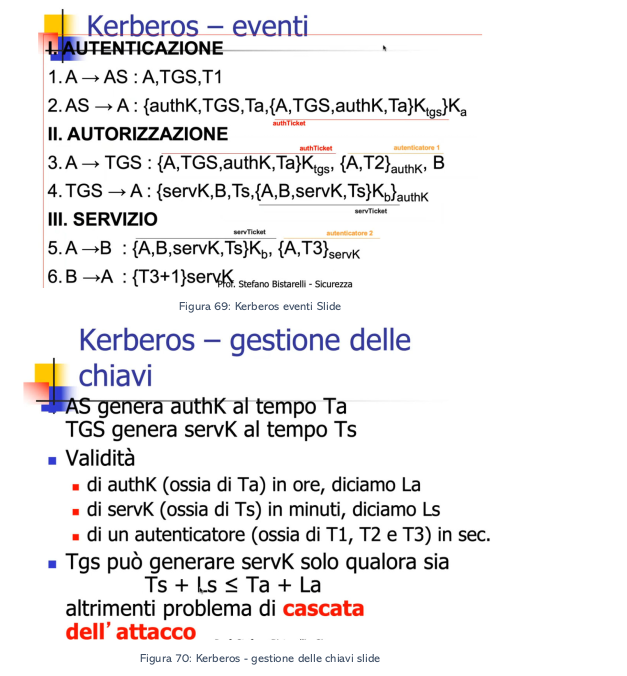
\includegraphics[width=7cm, keepaspectratio]{Bistarelli/img/keberos/keberos3.png}
\end{figure}

\begin{figure}[H]
	\centering
    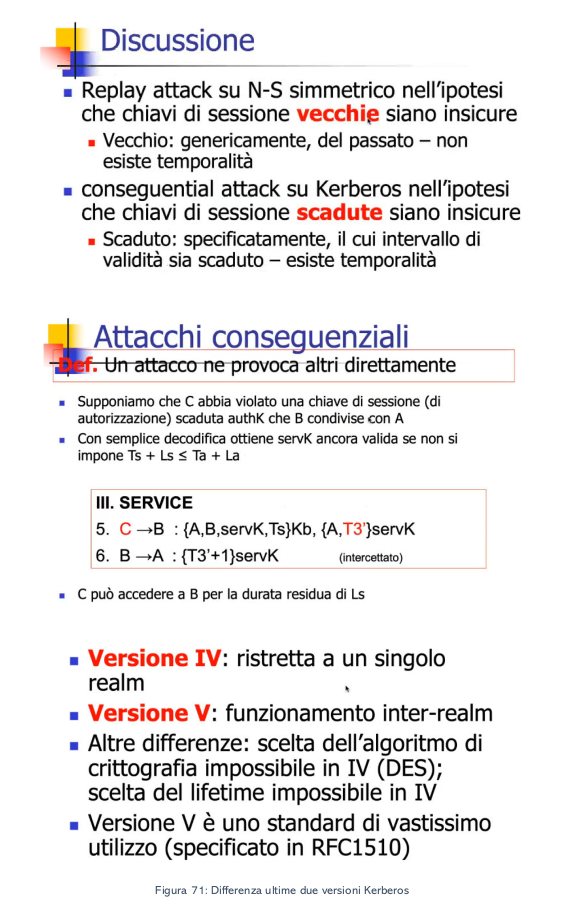
\includegraphics[width=7cm, keepaspectratio]{Bistarelli/img/keberos/keberos4.png}
\end{figure}

\begin{figure}[H]
	\centering
    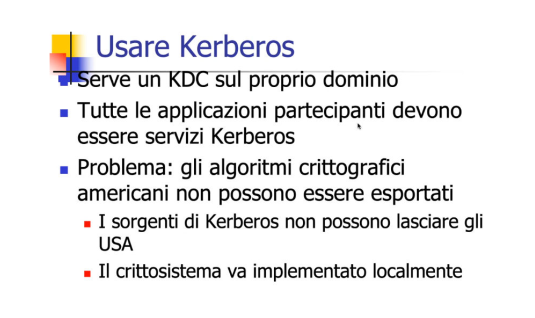
\includegraphics[width=7cm, keepaspectratio]{Bistarelli/img/keberos/keberos5.png}
\end{figure}
\subsection{Descrizione del protocollo}
Il client si autentica \textbf{sull'Authentication Server (AS)} che inoltra il nome utente a un centro di distribuzione
delle chiavi (KDC) . Il KDC emette un \textbf{ticket-granting ticket (TGT)} , che è timestamp e lo crittografa utilizzando la chiave segreta del \textbf{ticket-granting service (TGS)} e restituisce il risultato crittografato alla workstation dell'utente. Questa operazione viene eseguita raramente, in genere all'accesso dell'utente; il TGT scade a un certo punto sebbene possa essere rinnovato in modo trasparente dal gestore della sessione dell'utente mentre è
connesso. Quando il client ha bisogno di comunicare con un servizio su un altro nodo (un "principal", nel gergo
Kerberos), il client invia il \textbf{TGT} al \textbf{TGS}, che di solito condivide lo stesso host del KDC. Il servizio deve essere già stato registrato con il TGS con un nome dell'entità servizio (SPN) . Il client utilizza l'SPN per richiedere l'accesso a questo servizio. Dopo aver verificato che il TGT è valido e che l'utente è autorizzato ad accedere al servizio richiesto, il TGS emette il ticket e le chiavi di sessione al client. Il client invia quindi il ticket al \textbf{server del servizio (SS)} insieme alla sua richiesta di servizio.

\begin{figure}[H]
	\centering
    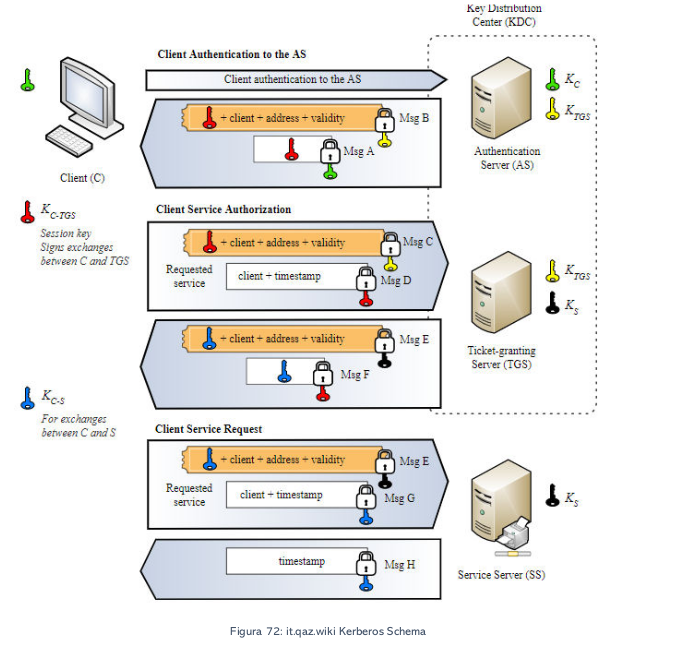
\includegraphics[width=7cm, keepaspectratio]{Bistarelli/img/keberos/keberos6.png}
\end{figure}
\subsection{Accesso basato su client utente}
Un utente immette un nome utente e una password sui computer client . Altri meccanismi di credenziali come
pkinit ( RFC 4556 ) consentono l'uso di chiavi pubbliche al posto di una password. Il client trasforma la password
nella chiave di un cifrario simmetrico. Questo utilizza la pianificazione della chiave incorporata o un hash
unidirezionale , a seconda della suite di crittografia utilizzata.
\subsection{Autenticazione client}
\begin{enumerate}
    \item Il client invia un messaggio di testo in chiaro dell'ID utente all'AS (Authentication Server) richiedendo servizi per conto dell'utente. (Nota: né la chiave segreta né la password vengono inviate all'AS.)
    
    \item L'AS verifica se il client è nel suo database. In tal caso, l'AS genera la chiave segreta eseguendo l'hashing della password dell'utente trovata nel database (ad esempio, Active Directory in Windows Server) e restituisce i seguenti due messaggi al client:
    
    \begin{itemize}
        \item Messaggio A: chiave di sessione client / TGS crittografata utilizzando la chiave segreta del client/ utente.
        
        \item Messaggio B: Ticket-Granting-Ticket (TGT, che include l'ID client, l' indirizzo di rete del client , il periodo di validità del ticket e la chiave di sessione client / TGS ) crittografato utilizzando la chiave segreta del TGS.
    \end{itemize}
    
    \item Una volta che il client riceve i messaggi A e B, tenta di decrittografare il messaggio A con la chiave segreta generata dalla password inserita dall'utente. Se la password inserita dall'utente non corrisponde alla password nel database AS, la chiave segreta del client sarà diversa e quindi non sarà in grado di decifrare il messaggio A. Con una password e una chiave segreta valide il client decrittografa il messaggio A per ottenere la chiave di sessione client / TGS . Questa chiave di sessione viene utilizzata per ulteriori comunicazioni con il TGS. (Nota: il client non può decrittografare il messaggio B, poiché è crittografato utilizzando la chiave segreta del TGS.) A questo punto, il client dispone di informazioni sufficienti per autenticarsi al TGS.
\end{enumerate}
\subsection{Autenticazione del servizio clienti}
\begin{enumerate}
    \item Quando richiede servizi, il client invia i seguenti messaggi al TGS:
    
    \begin{itemize}
        \item Messaggio C: composto dal messaggio B (il TGT crittografato che utilizza la chiave segreta TGS) e dall'ID del servizio richiesto.
        
        \item Messaggio D: Autenticatore (composto dall'ID client e dal timestamp), crittografato utilizzando la chiave di sessione client / TGS
    \end{itemize}
    
    \item Alla ricezione dei messaggi C e D, il TGS recupera il messaggio B dal messaggio C. Decrittografa il messaggio B utilizzando la chiave segreta TGS. Questo fornisce la "chiave di sessione client / TGS" e l'ID client (entrambi sono nel TGT). Utilizzando questa "chiave di sessione client / TGS", il TGS decrittografa il messaggio D (Authenticator) e confronta gli ID client dai messaggi B e D; se corrispondono, il server invia i seguenti due messaggi al client:
    
    \begin{itemize}
        \item Messaggio E: ticket da client a server (che include ID client, indirizzo di rete client, periodo di validità e chiave di sessione client / server ) crittografato utilizzando la chiave segreta del servizio.
        
        \item Messaggio F: chiave di sessione client / server crittografata con chiave di sessione client / TGS.
    \end{itemize}
\end{enumerate}
\subsection{Richiesta di servizio clienti}
\begin{enumerate}
    \item Dopo aver ricevuto i messaggi E ed F da TGS, il client dispone di informazioni sufficienti per autenticarsi al Service Server (SS). Il client si connette alla SS e invia i seguenti due messaggi:
    
    \begin{itemize}
        \item Messaggio E: dal passaggio precedente (il ticket da client a server , crittografato utilizzando la chiave segreta del servizio).
        
        \item Messaggio G: un nuovo autenticatore, che include l'ID client, il timestamp ed è crittografato utilizzando la chiave di sessione client / server.
    \end{itemize}
    
    \item L'SS decrittografa il ticket (messaggio E) utilizzando la propria chiave segreta per recuperare la chiave di sessione client / server . Utilizzando la chiave delle sessioni, SS decrittografa l'Autenticatore e confronta l'ID client dai messaggi E e G, se corrispondono, il server invia il seguente messaggio al client per confermare la sua vera identità e disponibilità a servire il client:
    
    \begin{itemize}
        \item Messaggio H: il timestamp trovato nell'autenticatore del client (più 1 nella versione 4, ma non necessario nella versione 5), crittografato utilizzando la chiave di sessione client / server.
    \end{itemize}
    
    \item Il client decrittografa la conferma (messaggio H) utilizzando la chiave di sessione client / server e controlla se il timestamp è corretto. In tal caso, il client può considerare attendibile il server e può iniziare a inviare richieste di servizio al server.
    
    \item Il server fornisce i servizi richiesti al client.
\end{enumerate}
\subsection{Inconvenienti e limitazioni}
\begin{itemize}
    \item Kerberos ha requisiti di tempo rigorosi, il che significa che gli orologi degli host coinvolti devono esseresincronizzati entro i limiti configurati. I ticket hanno un periodo di disponibilità temporale e se l'orologiodell'host non è sincronizzato con l'orologio del server Kerberos, l'autenticazione fallirà. La configurazione predefinita per MIT richiede che gli orari dell'orologio non siano distanti più di cinque minuti. In pratica , i demoni Network Time Protocol vengono solitamente utilizzati per mantenere sincronizzati gli orologi host. Si noti che alcuni server (l'implementazione di Microsoft è uno di questi) possono restituire un risultato KRB\_AP\_ERR\_SKEW contenente l'ora del server crittografata nel caso in cui entrambi gli orologi abbiano un offset maggiore del valore massimo configurato. In tal caso, il client potrebbe riprovare calcolando l'ora utilizzando l'ora del server fornita per trovare l'offset. Questo comportamento è documentato in RFC 4430.
    
    \item Il protocollo di amministrazione non è standardizzato e differisce tra le implementazioni del server. Le modifiche alla password sono descritte in RFC 3244
    
    \item In caso di adozione della crittografia simmetrica (Kerberos può funzionare utilizzando la crittografia simmetrica o asimmetrica (chiave pubblica)), poiché tutte le autenticazioni sono controllate da un centro di distribuzione delle chiavi centralizzato (KDC), la compromissione di questa infrastruttura di autenticazione consentirà a un utente malintenzionato di impersonare qualsiasi utente
    
    \item Ogni servizio di rete che richiede un nome host diverso avrà bisogno del proprio set di chiavi Kerberos. Ciò complica l'hosting virtuale e i cluster.
    
    \item Kerberos richiede che gli account utente e i servizi abbiano una relazione affidabile con il server di token Kerberos.
    
    \item La fiducia del client richiesta rende difficile la creazione di ambienti a fasi (ad esempio, domini separati per l'ambiente di test, l'ambiente di pre-produzione e l'ambiente di produzione): è necessario creare relazioni di fiducia del dominio che impediscano una netta separazione dei domini dell'ambiente o che siano necessari client utente aggiuntivi previsto per ogni ambiente.
\end{itemize}
\subsection{Vulnerabilità}
La crittografia Data Encryption Standard (DES) può essere utilizzata in combinazione con Kerberos, ma non è più uno standard Internet perché è debole. Esistono vulnerabilità di sicurezza in molti prodotti legacy che implementano Kerberos perché non sono stati aggiornati per utilizzare crittografie più recenti come AES invece di DES. Nel novembre 2014, Microsoft ha rilasciato una patch (MS14-068) per correggere una vulnerabilità sfruttabile nell'implementazione Windows del Kerberos Key Distribution Center (KDC). La vulnerabilità presumibilmente consente agli utenti di "elevare" (e abusare) i propri privilegi, fino al livello di dominio.
\subsection{Altra descrizione del protocollo (wikipedia)}
In informatica e telecomunicazioni Kerberos è un protocollo di rete per l'autenticazione forte che permette a diversi
terminali di comunicare su una rete informatica insicura provando la propria identità mediante l'utilizzo di tecniche
di crittografia simmetrica. Kerberos previene attacchi quali l'intercettazione e i replay attack ed assicura l'integrità
dei dati. I suoi progettisti mirarono soprattutto ad un modello client-server, e fornisce una mutua autenticazione
cioè sia l'utente sia il fornitore del servizio possono verificare l'identità dell'altro.
\subsubsection{Descrizione}
Kerberos si basa sul protocollo di Needham-Schroeder. Utilizza una terza parte affidabile per centralizzare la
distribuzione delle chiavi detta Key Distribution Center (KDC), che consiste di due parti separate logicamente:
l'Authentication Server (AS) e il Ticket Granting Server (TGS). Kerberos funziona utilizzando dei "biglietti" (detti
ticket) che servono per provare l'identità degli utenti.

\singlespacing

L'AS mantiene un database delle chiavi segrete; ogni entità sulla rete — che sia un client o un server — condivide
la chiave segreta solo con l'AS. La conoscenza di questa chiave serve per provare l'identità di un'entità. Per
comunicazioni tra due entità, Kerberos genera una chiave di sessione, che può essere utilizzata dai due terminali
per comunicare.

\subsubsection{Il protocollo}
Il protocollo può essere definito come segue utilizzando la notazione per protocolli di sicurezza, dove Alice (A) si
autentica presso Bob (B) usando il server S:

\begin{figure}[H]
	\centering
    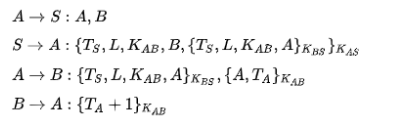
\includegraphics[width=7cm, keepaspectratio]{Bistarelli/img/keberos/keberos7.png}
\end{figure}

La sicurezza del protocollo si basa fortemente sui timestamp T e sui tempi di vita L come indicatori affidabili della
creazione recente della comunicazione per evitare replay attack (vedi logica BAN).

\singlespacing

È importante notare come il server S stia sia come Authentication Service (AS) sia come Ticket Granting Service
(TGS).

\begin{figure}[H]
	\centering
    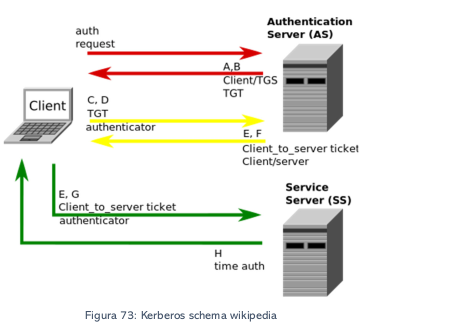
\includegraphics[width=7cm, keepaspectratio]{Bistarelli/img/keberos/keberos8.png}
\end{figure}
\subsubsection{Operazioni di Kerberos}
Quella che segue è una descrizione semplificata del protocollo. Saranno utilizzate le seguenti abbreviazioni: AS =
Authentication Server, TGS = Ticket Granting Server, SS = Service Server.In breve: il client si autentica presso AS
che gli fornisce un ticket di sessione per accedere a TGS, si autentica presso TGS e riceve il ticket per aprire una
sessione di comunicazione con SS. In dettaglio
\subsubsection{Utente: autenticazione di base}
\begin{enumerate}
    \item Un utentie inserisce username e password sul client
\end{enumerate}
\subsubsection{Client: Autenticazione AS}
\begin{enumerate}
    \item Il client manda un messaggio non criptato all'AS richiedendo i servizi per l'utente. ("L'utente XYZ vorrebbe richiedere dei servizi"). Né la chiave segreta né la password vengono inviate all'AS.
    
    \item L'AS controlla se il client è nel suo database. Se lo è invia due messaggi al client:
    
    \begin{itemize}
        \item Messaggio A: Chiave di sessione client-TGS criptata usando la chiave segreta dell'utente.
        
        \item Messaggio B: Ticket-Granting Ticket (che include l'identificativo del client, l'indirizzo di rete, il tempo di validità del ticket e la chiave di sessione client-TGS). Il Ticket-Granting Ticket è criptato utilizzando la chiave segreta di TGS.
    \end{itemize}
    
    \item Quando il client riceve i messaggi A e B, decripta il messaggio A ottenendo la chiave di sessione client-TGS. Questa chiave è utilizzata per le successive comunicazioni con TGS. (Nota: il client non può decriptare il Messaggio B, che è stato criptato con la chiave segreta di TGS). A questo punto il client possiede i mezzi per autenticarsi presso TGS.
\end{enumerate}
\subsubsection{Client: Autenticazione TGS}
\begin{enumerate}
    \item Quando richiede dei servizi, il client invia i seguenti due messaggi a TGS:
    \begin{itemize}
        \item Messaggio C: composto dal Ticket-Granting Ticket (mandatogli dal AS nel messaggio B) e dall'identificativo del servizio richiesto
        
        \item Messaggio D: autenticatore (Authenticator) (che è formato da identificativo del client e imestamp), criptato usando la chiave di sessione client—TGS.
    \end{itemize}
    \item Ricevendo i messaggi C e D, TGS decripta il messaggio C con la propria chiave e dal messaggio estrae la chiave di sessione client—TGS che utilizza per decriptare il messaggio D (autenticatore). A questo punto invia i seguenti due messaggi al client:
    \begin{itemize}
        \item Messaggio E: Ticket client-server (che include l'identificativo del client, l'indirizzo di rete del client, il periodo di validità e la chiave di sessione client-server) criptato utilizzando la chiave segreta del server che offre il servizio.
        
        \item Messaggio F: Chiave di sessione client-server criptato usando la chiave di sessione client-TGS
    \end{itemize}
\end{enumerate}
\subsubsection{Client: Autenticazione SS}
\begin{enumerate}
    \item Ricevendo i messaggi E e F dal TGS, il client può autenticarsi presso il SS. Il client si connette al SS e invia i seguenti due messaggi:
    
    \begin{itemize}
        \item Messaggio E: Ticket client-server criptato usando la chiave segreta di SS.
        
        \item Messaggio G: un nuovo autenticatore, che include l'identificativo del client, il timestamp ed è
    \end{itemize}
    
    \item Il server decripta il ticket usando la sua chiave segreta e invia il seguente messaggio al client per confermare la propria identità e la volontà di fornire il servizio al client:
    
    \begin{itemize}
        \item Messaggio H: il timestamp trovato nell'autenticatore incrementato di uno, criptato utilizzando la chiave di sessione client-server.
    \end{itemize}
    
    \item Il client decripta la conferma usando la chiave di sessione client-server e controlla che il timestamp sia correttamente aggiornato. Se lo è, il client può considerare affidabile il server e iniziare a effettuare le richieste di servizio.
    
    \item Il server fornisce i servizi al client.
    
    
\end{enumerate}
    \newpage
\chapter*{Capitolo4}
\section{Principi di controllo dell'accesso}
Due definizioni di controllo dell'accesso sono utili per capire la sua portata.
\begin{enumerate}
    \item \textbf{NISTIR 7298} (Glossario dei termini chiave della sicurezza delle informazioni, maggio 2013), definisce il controllo dell'accesso come il processo di concessione o rifiuto di richieste specifiche a:
    
    \begin{itemize}
        \item  Ottenere e utilizzare le informazioni e i relativi servizi di elaborazione delle informazioni
        
        \item  Entrare in specifiche strutture fisiche.
    \end{itemize}
    
    \item \textbf{RFC 4949}, Internet Security Glossary, definisce il controllo dell'accesso come un processo con cui l'uso delle risorse del sistema è regolato secondo una politica di sicurezza è permesso solo alle entità autorizzate (utenti, programmi, processi o altri sistemi) secondo tale politica.
    
Possiamo considerare il controllo degli accessi come un elemento centrale della sicurezza informatica. Gli obiettivi principali della sicurezza informatica sono di impedire agli utenti non autorizzati di accesso alle risorse, impedire agli utenti legittimi di accedere alle risorse in modo non in modo non autorizzato, e permettere agli utenti legittimi di accedere alle risorse in modo autorizzato.

\begin{figure}[H]
	\centering
    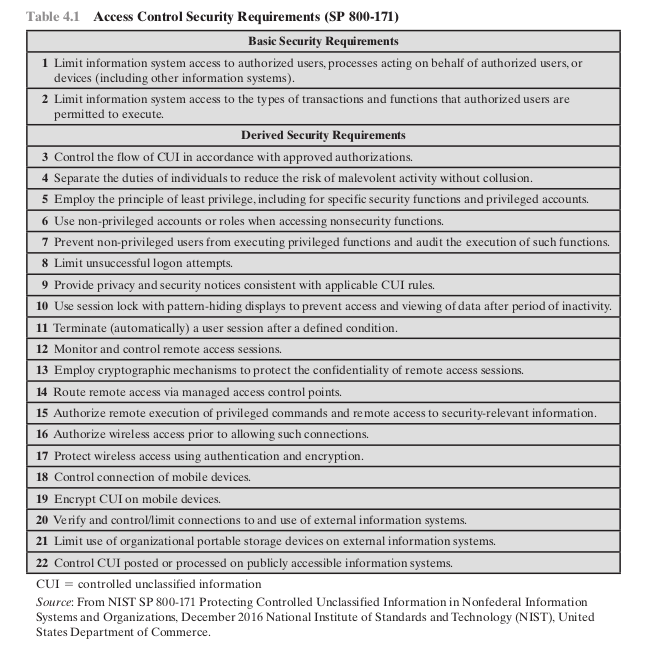
\includegraphics[width=14cm, keepaspectratio]{Bistarelli/img/cap_4/tabella4.1.png}
\end{figure}

In senso lato, tutta la sicurezza informatica riguarda il controllo degli accessi. Infatti, RFC 4949 definisce la sicurezza informatica come segue:

\begin{center}
    \textbf{Misure che implementano e assicurano servizi di sicurezza in un sistema informatico, in particolare quelle che assicurano il servizio di controllo degli accessi.}
\end{center}
\end{enumerate}
\newpage
\subsection{Contesto del controllo dell'accesso}
Oltre al controllo d'accesso, questo contesto coinvolge le seguenti entità e funzioni:
\begin{itemize}
    \item \textbf{Autenticazione}
    
    Verifica che le credenziali di un utente o di un'altra entità del sistema siano valide.
    
    \item \textbf{Autorizzazione}
    
    La concessione di un diritto o di un permesso ad un'entità di sistema per accedere una risorsa del sistema. Questa funzione determina chi è affidabile per un determinato scopo.
    
    \item \textbf{Audit}
    
    Una revisione ed esame indipendente delle registrazioni e delle attività del sistema al fine di verificare l'adeguatezza dei controlli del sistema, di assicurare la conformità con con la politica stabilita e le procedure operative, per rilevare le violazioni della sicurezza, e per raccomandare qualsiasi cambiamento indicato nel controllo, nella politica e nelle procedure.

\end{itemize}
Un meccanismo di controllo dell'accesso media tra un utente (o un processo che esegue per conto di un utente) e le risorse di sistema, come applicazioni, sistemi operativi, firewall, router, file e database. Il sistema deve prima autenticare un'entità che cerca l'accesso. Tipicamente, la funzione di autenticazione determina se l'utente è permesso di accedere al sistema. Poi la funzione di controllo dell'accesso determina se l'accesso specifico richiesto da questo utente è permesso. Un amministratore di sicurezza mantiene un database un database di autorizzazioni che specifica quale tipo di accesso a quali risorse è permesso a questo utente. La funzione di controllo degli accessi consulta questo database per se concedere l'accesso. Una funzione di auditing monitora e tiene un registro degli accessi degli utenti alle risorse del sistema.
\singlespacing
In pratica, un certo numero di componenti può cooperare per condividere la funzione di controllo la funzione di controllo degli accessi. Tutti i sistemi operativi hanno almeno un rudimentale, e in molti casi un componente di controllo degli accessi abbastanza robusto. I pacchetti di sicurezza aggiuntivi possono integrare le capacità di controllo d'accesso native del sistema operativo. Applicazioni particolari o utilità, come un sistema di gestione di database, incorporano anche funzioni di controllo degli accessi funzioni di controllo degli accessi. Dispositivi esterni, come i firewall, possono anche fornire servizi di controllo dell'accesso.
\newpage
\subsection{Politiche di controllo dell'accesso}
Una politica di controllo degli accessi, che può essere incorporata in un database di autorizzazioni, quali tipi di accesso sono permessi, in quali circostanze e da chi.
\singlespacing
Le politiche di controllo dell'accesso sono generalmente raggruppate nelle seguenti categorie:
\begin{itemize}
    \item \textbf{Controllo dell'accesso discrezionale (DAC)}
    
    Controlla l'accesso in base all'identità del richiedente e su regole di accesso (autorizzazioni) che stabiliscono cosa i richiedenti sono (o non sono)autorizzati a fare. Questa politica è definita discrezionale perché un'entità può avere diritti di accesso che permettono all'entità, di sua spontanea volontà, di un'altra entità di accedere a qualche risorsa.
    
    \item \textbf{Controllo di accesso obbligatorio (MAC)}
    
    
    Controlla l'accesso basandosi sul confronto delle etichette di sicurezza (che indicano quanto sono sensibili o critiche le risorse del sistema) con le autorizzazioni di sicurezza (che indicano le entità del sistema). con le autorizzazioni di sicurezza (che indicano che le entità del sistema sono autorizzate ad accedere a certe risorse). risorse). Questa politica è definita obbligatoria perché un'entità che ha l'autorizzazione di accedere a una risorsa non può, solo per sua volontà, permettere a un'altra entità di accedere a quella risorsa.
    
    \item \textbf{Controllo di accesso basato sui ruoli (RBAC)}
    
    Controlla l'accesso in base ai ruoli che gli utenti hanno all'interno del sistema e su regole che stabiliscono quali accessi sono permessi agli utenti in determinati ruoli.
    
    \item \textbf{Controllo di accesso basato sugli attributi (ABAC)}
    
    Controlla l'accesso in base agli attributi dell'utente, della risorsa a cui accedere e delle condizioni ambientali correnti.
\end{itemize}
\singlespacing
Queste quattro politiche non si escludono a vicenda. Un meccanismo di controllo degli accessi può impiegare due o anche tutte e tre queste politiche per coprire diverse classi di risorse di sistema.
\newpage
\subsection{Soggetti oggetti e diritti d'accesso}
Gli elementi di base del controllo d'accesso sono: soggetto, oggetto e diritto d'accesso.
\singlespacing
Un soggetto è un'entità capace di accedere agli oggetti. In generale, il concetto di soggetto equivale a quello di processo. Qualsiasi utente o applicazione ottiene effettivamente l'accesso a un oggetto per mezzo di un processo che rappresenta quell'utente o applicazione. Il processo assume gli attributi dell'utente, come i diritti di accesso.
\singlespacing
Un soggetto è tipicamente ritenuto responsabile delle azioni che ha iniziato, e un audit trail può essere usato per registrare l'associazione di un soggetto con azioni rilevanti per la sicurezza eseguite su un oggetto dal soggetto.
I sistemi di controllo dell'accesso di base definiscono tipicamente tre classi di soggetti, con diritti di accesso diversi per ogni classe:
\begin{itemize}
    \item \textbf{Propietario:} può essere il creatore di una risorsa, come un file. Per le risorse di sistema, la proprietà può appartenere ad un amministratore di sistema. Per le risorse del progetto, l'amministratore o il un amministratore di progetto o un leader può essere assegnato la proprietà.
    
    \item \textbf{Gruppo:} In aggiunta ai privilegi assegnati ad un proprietario, ad un gruppo nominato di utenti possono anche essere concessi diritti di accesso, in modo tale che l'appartenenza al gruppo sufficiente per esercitare questi diritti di accesso. Nella maggior parte degli schemi, un utente può appartenere a più gruppi.
    
    \item \textbf{Mondo:} Il minimo di accesso è concesso agli utenti che sono in grado di accedere al sistema ma non sono inclusi nelle categorie proprietario e gruppo per questa risorsa.
\end{itemize}
Un oggetto è una risorsa il cui accesso è controllato. In generale, un oggetto è un'entità usata per contenere e/o ricevere informazioni.
\singlespacing
Il numero e i tipi di oggetti da proteggere con un sistema di controllo degli accessi dipende dall'ambiente in cui opera il controllo degli accessi e dal compromesso tra sicurezza da un lato e complessità, carico di lavoro e facilità d'uso dall'altro.
\singlespacing
Un diritto di accesso descrive il modo in cui un soggetto può accedere a un oggetto.
\singlespacing
I diritti di accesso potrebbero includere quanto segue:
\begin{itemize}
    \item \textbf{Leggere:} L'utente può visualizzare le informazioni in una risorsa di sistema (ad esempio, un file, record selezionati record in un file, campi selezionati all'interno di un record, o qualche combinazione). Lettura l'accesso include la possibilità di copiare o stampare.
    
    \item \textbf{Scrittura:} L'utente può aggiungere, modificare o cancellare dati in una risorsa di sistema (ad esempio, file, record, programmi). L'accesso in scrittura include l'accesso in lettura.
    
    \item \textbf{Eseguire:} L'utente può eseguire programmi specifici.
    
    \item \textbf{Cancellare:} L'utente può cancellare certe risorse di sistema, come file o record.
    
    \item \textbf{Creare:} L'utente può creare nuovi file, record o campi.
    
    \item \textbf{Cercare:} L'utente può elencare i file in una directory o altrimenti cercare nella directory.
\end{itemize}
\subsection{Controllo dell'accesso discrezionale}
Come si è detto in precedenza, uno schema di controllo di accesso discrezionale è uno schema in cui un'entità può ricevere diritti di accesso che le permettono, per sua volontà, di permettere a un'altra entità di accedere a qualche risorsa. Un approccio generale al DAC, come esercitato da un sistema operativo o da un sistema di gestione di database, è quello di una matrice di accesso.
\begin{center}
    \textbf{Una dimensione della matrice consiste in soggetti identificati che possono tentare l'accesso alle risorse.}
\end{center}
Tipicamente, questa lista consisterà di singoli utenti o gruppi di utenti anche se l'accesso potrebbe essere controllato per terminali, apparecchiature di rete, host, o applicazioni invece di o in aggiunta agli utenti. L'altra dimensione elenca gli oggetti a cui si può accedere. Al massimo livello di dettaglio, gli oggetti possono essere singoli dati campi di dati. Raggruppamenti più aggregati, come record, file o anche l'intero database, possono anche essere oggetti nella matrice. Ogni voce nella matrice indica i diritti di accesso di un particolare soggetto per un particolare oggetto.

\begin{figure}[H]
	\centering
    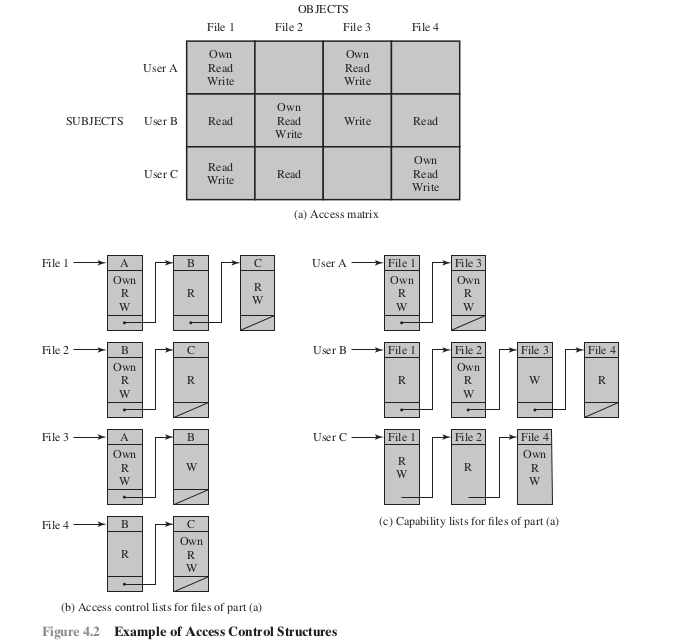
\includegraphics[width=14cm, keepaspectratio]{Bistarelli/img/cap_4/figura4.2.png}
\end{figure}

Così, l'utente A possiede i file 1 e 3 e ha diritti di accesso in lettura e scrittura a questi file. L'utente B ha diritti di accesso in lettura al file 1, e così via.

\singlespacing

In pratica, una matrice di accesso è di solito sparsa e viene implementata con la decomposizione in uno dei due modi. La matrice può essere decomposta per colonne, ottenendo liste di controllo degli accessi (ACL) (vedi Figura 4.2b). Per ogni oggetto, una ACL elenca gli utenti e i loro diritti di accesso consentiti. L'ACL può contenere una voce di default, o pubblica. Questo permette agli utenti che non sono esplicitamente elencati come aventi diritti speciali di avere un set di diritti. L'insieme predefinito di diritti dovrebbe sempre seguire la regola del minimo privilegio o accesso in sola lettura, a seconda del caso. Gli elementi della lista possono includere singoli utenti così come gruppi di utenti.

\singlespacing

Quando si vuole determinare quali soggetti hanno quali diritti di accesso ad una particolare risorsa, le ACL sono convenienti, perché ogni ACL fornisce le informazioni per una data risorsa. Tuttavia, questa struttura di dati non è conveniente per determinare i diritti di accesso disponibili per uno specifico utente.

\singlespacing

La decomposizione per righe produce i capability ticket (vedi Figura 4.2c).

\singlespacing

Un capability è un ticket di capacità specifica gli oggetti e le operazioni autorizzate per un particolare utente. Ogni utente ha un certo numero di ticket e può essere autorizzato a prestarli o darli ad altri. Poiché i ticket possono essere dispersi nel sistema, presentano un problema di sicurezza maggiore rispetto alle liste di controllo degli accessi. L'integrità del ticket deve essere protetta e garantita (di solito dal sistema operativo). In particolare, il ticket deve essere non falsificabile. Un modo per ottenere ciò è quello di avere il sistema operativo che tiene tutti i ticket per conto degli utenti. Questi biglietti dovrebbero essere tenuti in una regione di memoria inaccessibile agli utenti. Un'altra alternativa è includere un token non falsificabile nella capacità. Questo potrebbe essere una grande password casuale, o un codice crittografico di autenticazione del messaggio. Questo valore è verificato dalla risorsa ogni volta che viene richiesto l'accesso. Questa forma di capability ticket è appropriata per Questa forma di capability ticket è appropriata per l'uso in un ambiente distribuito, quando la sicurezza del suo contenuto non può essere garantita. Gli aspetti convenienti e scomodi dei capability ticket sono l'opposto di quelli delle ACL. È facile determinare l'insieme dei diritti di accesso che un dato utente ha, ma è più difficile determinare l'elenco degli utenti con diritti di accesso specifici per una risorsa specifica.

\singlespacing

Una tabella di autorizzazione contiene una riga per un diritto di accesso di un soggetto ad una risorsa. Ordinare o accedere alla tabella per soggetto è equivalente a una lista di capacità. Ordinare o l'accesso alla tabella per oggetto è equivalente ad una ACL. Un database relazionale può facilmente implementare una tabella di autorizzazione di questo tipo.

\begin{figure}[H]
	\centering
    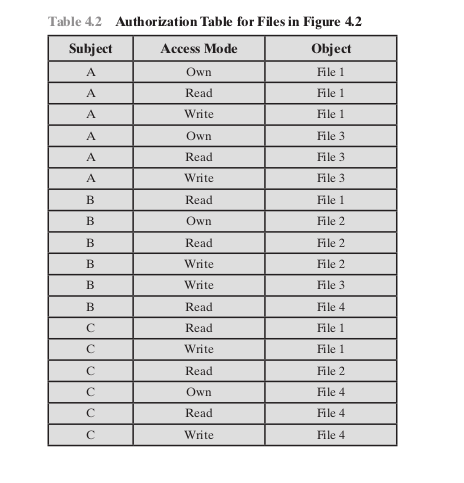
\includegraphics[width=14cm, keepaspectratio]{Bistarelli/img/cap_4/tabella4.2.png}
\end{figure}
\newpage
\subsection{Un modello di controllo d'accesso}
Questa sezione introduce un modello generale per DAC sviluppato da Lampson, Graham, e Denning. Il modello presuppone un insieme di soggetti, un insieme di oggetti e un insieme di regole che governano l'accesso dei soggetti agli oggetti. Definiamo lo stato di protezione di un sistema come l'insieme di informazioni, in un dato momento, che specifica i diritti di accesso per ogni soggetto rispetto a ogni oggetto.

\singlespacing

Noi Possiamo identificare tre requisiti: rappresentare lo stato di protezione, far rispettare i diritti di accesso e permettere ai soggetti di alterare lo stato di protezione in certi modi. Il modello affronta tutti e tre i requisiti, dando una descrizione generale e logica di un sistema DAC.

\singlespacing

Per rappresentare lo stato di protezione, estendiamo l'universo di oggetti nella matrice di controllo degli accessi per includere quanto segue:
\begin{itemize}
    \item \textbf{Processi:} I diritti di accesso includono la capacità di cancellare un processo, fermare (bloccare) e svegliare un processo.

    \item \textbf{Dispositivi:} I diritti di accesso includono la capacità di leggere/scrivere il dispositivo, di controllare il suo funzionamento (ad esempio, una ricerca su disco), e di bloccare/sbloccare il dispositivo per l'uso.
    
    \item \textbf{Luoghi o regioni di memoria:} I diritti di accesso includono la capacità di leggere/scrivere certe regioni di memoria che sono protette in modo tale che il default è di disabilitare l'accesso.
    
    \item \textbf{Soggetti:} I diritti di accesso rispetto ad un soggetto hanno a che fare con la capacità di concedere o cancellare i diritti di accesso di quel soggetto ad altri oggetti, come spiegato successivamente.
\end{itemize}
La figura 4.3 è un esempio. Per una matrice di controllo di accesso A, ogni voce A[S, X] contiene stringhe, chiamate attributi di accesso, che specificano i diritti di accesso del soggetto S all per l'oggetto X. Per esempio, nella figura 4.3, S1 può leggere il file F1, perché 'read' appare in A[S1, F1]. Da un punto di vista logico o funzionale, un modulo di controllo degli accessi separato è associato ad ogni tipo di oggetto (vedi figura 4.4). Il modulo valuta ogni Il modulo valuta ogni richiesta di un soggetto di accedere a un oggetto per determinare se il diritto di accesso esiste. Un tentativo di accesso innesca i seguenti passi:
\begin{enumerate}
    \item Un soggetto S0 emette una richiesta di tipo a per l'oggetto X.
    
    \item La richiesta fa sì che il sistema (il sistema operativo o un modulo di interfaccia di controllo degli accessi di qualche tipo) a generare un messaggio della forma (S0, a, X) al controllore per X.
    
    \item Il controllore interroga la matrice di accesso A per determinare se a è in A[S0, X].
\end{enumerate}

\begin{figure}[H]
	\centering
    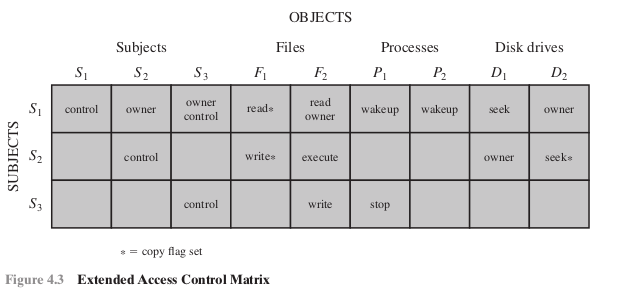
\includegraphics[width=14cm, keepaspectratio]{Bistarelli/img/cap_4/figura4.3.png}
\end{figure}

In caso affermativo, l'accesso è permesso; in caso contrario, l'accesso è negato e si verifica una violazione della protezione si verifica una violazione della protezione. La violazione dovrebbe innescare un avvertimento e un'azione appropriata.

\singlespacing

La figura 4.4 suggerisce che ogni accesso di un soggetto ad un oggetto è mediato dal controllore per quell'oggetto, e che la decisione del controllore è basata sul contenuto attuale della matrice. Inoltre, alcuni soggetti hanno l'autorità di apportare modifiche specifiche alla matrice di accesso. Una richiesta di modifica della matrice di accesso è trattata come un accesso alla matrice, con le singole voci della matrice trattate come oggetti.

\singlespacing

Tali accessi sono mediati da un controllore della matrice di accesso, che controlla gli aggiornamenti alla matrice. Il modello include anche un insieme di regole che governano le modifiche alla matrice di accesso come mostrato nella tabella 4.3. A questo scopo, introduciamo i diritti di accesso "proprietario e 'controllo' e il concetto di flag di copia, come spiegato nei paragrafi successivi.

\singlespacing

Le prime tre regole riguardano il trasferimento, la concessione e la cancellazione dei diritti di accesso. Supponiamo che la voce a* esista in A[S0, X]. Questo significa che S0 ha il diritto di accesso a al soggetto X e, a causa della presenza del flag di copia, può trasferire questo diritto, con o senza con o senza flag di copia, ad un altro soggetto. La regola R1 esprime questa capacità. Un soggetto potrebbe trasferire il diritto di accesso senza il flag di copia se ci fosse la preoccupazione che il nuovo soggetto potrebbe trasferire maliziosamente il diritto ad un altro soggetto che non dovrebbe avere quel diritto di accesso. Per esempio, S1 può mettere 'read' o 'read*' in qualsiasi voce della matrice in nella colonna F1. La regola R2 afferma che se S0 è designato come proprietario dell'oggetto X, allora S0 può concedere un diritto di accesso a quell'oggetto per qualsiasi altro soggetto. La regola R2 afferma che che se S0 è designato come proprietario dell'oggetto X, allora S0 può concedere un diritto di accesso a quell'oggetto per qualsiasi altro soggetto.

\singlespacing

\paragraph{La regola R2} afferma che S0 può aggiungere qualsiasi diritto di accesso ad A[S, X] per qualsiasi S, se S0 ha accesso "proprietario" a X. La regola R3 permette a S0 di cancellare qualsiasi diritto di accesso da qualsiasi voce della matrice in una riga per la quale S0 controlla il soggetto, e per qualsiasi voce della matrice in una colonna per la quale S0 possiede l'oggetto.

\singlespacing

\paragraph{La regola R4} permette ad un soggetto di leggere quella porzione di matrice che possiede o controlla.

\singlespacing

Le restanti regole della tabella 4.3 regolano la creazione e la cancellazione di soggetti e oggetti.

\singlespacing

\paragraph{La regola R5} afferma che ogni soggetto può creare un nuovo oggetto, che possiede, e può quindi concedere e cancellare l'accesso all'oggetto. Secondo la regola R6, il proprietario di un oggetto può distruggere l'oggetto, con la conseguente cancellazione della colonna corrispondente della matrice di accesso.

\singlespacing

\paragraph{La regola R7} permette a qualsiasi soggetto di creare un nuovo soggetto; il creatore è proprietario del nuovo soggetto e il nuovo soggetto ha accesso di controllo su se stesso.

\singlespacing

\paragraph{La regola R8} permette al proprietario di un soggetto di cancellare la riga e la colonna (se ci sono colonne di soggetti) della matrice di accesso designata da quel soggetto.

\singlespacing

L'insieme di regole nella Tabella 4.3 è un esempio dell'insieme di regole che potrebbero essere definite per un sistema di controllo degli accessi. I seguenti sono esempi di regole aggiuntive o alternative

\begin{figure}[H]
	\centering
    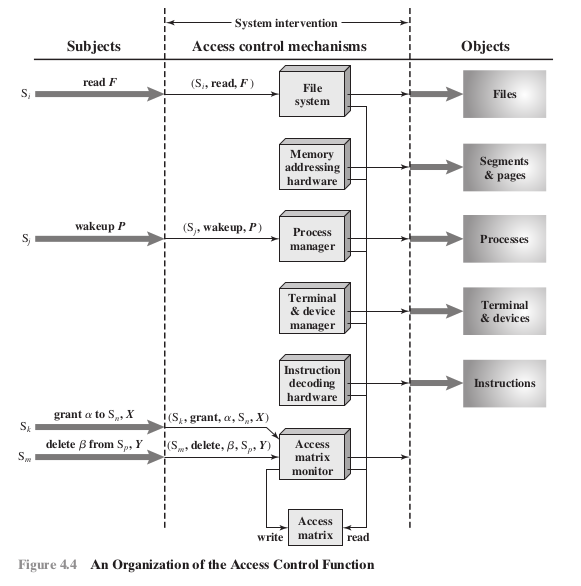
\includegraphics[width=14cm, keepaspectratio]{Bistarelli/img/cap_4/figura4.4.png}
\end{figure}

\begin{figure}[H]
	\centering
    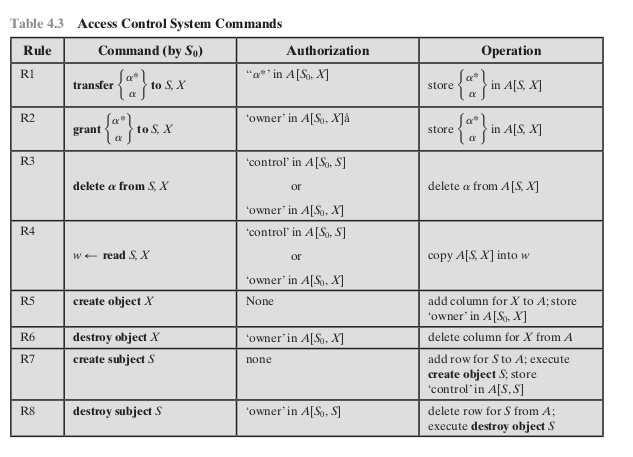
\includegraphics[width=14cm, keepaspectratio]{Bistarelli/img/cap_4/tabella4.3.png}
\end{figure}
\section{Esempio: Controllo di accesso ai file Unix}
Tutti i tipi di file UNIX sono amministrati dal sistema operativo per mezzo di inode.
\singlespacing
\textbf{Un inode} (nodo indice) è una struttura di controllo che contiene le informazioni chiave necessarie al sistema operativo per un particolare file. Diversi nomi di file possono essere associati ad un singolo inode, ma un inode attivo è associato esattamente ad un file, e ogni file è controllato esattamente da un inode. Gli attributi del file così come i suoi permessi e altre informazioni di controllo sono memorizzati nell'inode. Sul disco, c'è una tabella di inode, o lista di inode, che contiene gli inode di tutti i file nel file sistema. Quando un file viene aperto, il suo inode viene portato nella memoria principale e memorizzato in una tabella di inode residente in memoria.
\singlespacing
Le directory sono strutturate in un albero gerarchico. Ogni directory può contenere file e/o altre directory. Una directory che si trova all'interno di un'altra directory viene una sottodirectory. Una directory è semplicemente un file che contiene una lista di nomi di file più puntatori agli inode associati. Così, associato ad ogni directory c'è il proprio inode.
\subsection{Controllo di accesso ai file UNIX tradizionale}
La maggior parte dei sistemi UNIX dipende, o almeno si basa, sullo schema di controllo dell'accesso ai file introdotto con le prime versioni di UNIX. Ad ogni utente UNIX viene assegnato un unico numero di identificazione utente (ID utente). Un utente è anche membro di un gruppo primario, e possibilmente di un certo numero di altri gruppi, ciascuno identificato da un ID di gruppo. Quando un file viene creato, è designato come di proprietà di un particolare utente e contrassegnato dall'ID di quell'utente \textbf{ID DI QUELL'UTENTE}.
\singlespacing
Appartiene anche a un gruppo specifico, che inizialmente è o il gruppo primario del suo creatore, o il gruppo della sua directory madre se questa ha il permesso SetGID impostato. Associato ad ogni file c'è un insieme di 12 bit di protezione. L'ID del proprietario, l'ID del gruppo e i bit di protezione fanno parte dell'inode del file.
\singlespacing
Nove dei bit di protezione specificano i permessi di lettura, scrittura ed esecuzione per il proprietario del file, gli altri membri del gruppo a cui questo file appartiene e tutti gli altri utenti. Questi formano una gerarchia di proprietario, gruppo e tutti gli altri, con l'insieme di permessi più alto che viene usato. La figura 4.5a mostra un esempio in cui il proprietario del file ha accesso in lettura e scrittura; tutti gli altri membri del gruppo del file hanno accesso in lettura; e gli utenti esterni al gruppo non hanno diritti di accesso al file. Quando sono applicati ad una directory, i bit di lettura e scrittura garantiscono il diritto di elencare e creare/rinominare/cancellare file nella directory. Il bit di esecuzione garantisce il diritto di scendere nella directory o di cercare un nome di file.

\begin{figure}[H]
	\centering
    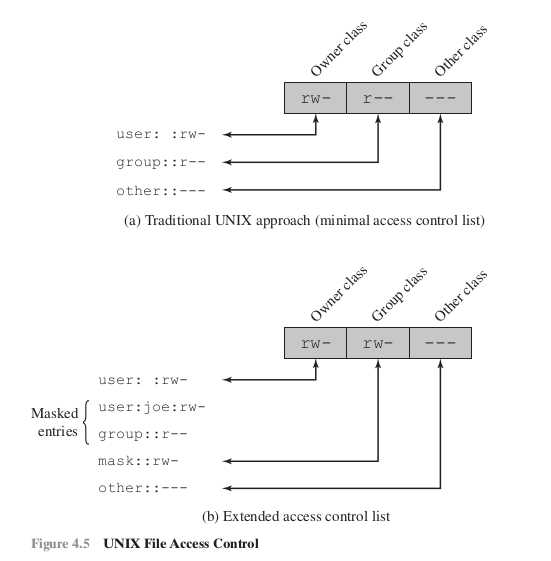
\includegraphics[width=14cm, keepaspectratio]{Bistarelli/img/cap_4/figura4-5.png}
\end{figure}

I tre bit rimanenti definiscono uno speciale comportamento aggiuntivo per i file o le directory. Due di questi sono i permessi "set user ID" (SetUID) e "set group ID" (SetGID) permessi. Se questi sono impostati su un file eseguibile, il sistema operativo funziona come segue.

\singlespacing

Quando un utente (con privilegi di esecuzione per questo file) esegue il file, il sistema alloca temporaneamente i diritti dell'ID dell'utente del creatore del file, o del gruppo del file, rispettivamente, a quelli dell'utente che esegue il file. Questi sono conosciuti come "ID utente effettivo" e "ID gruppo effettivo" e sono usati in aggiunta all'"ID utente reale" e all'"ID gruppo reale". "ID" e "ID gruppo reale" dell'utente in esecuzione quando si prendono decisioni di controllo dell'accesso per questo programma. Questa modifica è efficace solo mentre il programma è in esecuzione.

\singlespacing

Questa caratteristica permette la creazione e l'uso di programmi privilegiati che possono utilizzare file normalmente inaccessibili agli altri utenti. Permette agli utenti di accedere a certi file in modo con controllato. In alternativa, quando applicato ad una directory, il permesso SetGID indica che i file appena creati erediteranno il gruppo di questa directory. Il permesso SetUID viene ignorata.

\singlespacing

L'ultimo bit di permesso è il bit "appiccicoso". Quando è impostato su un file, originariamente indica che il sistema dovrebbe mantenere il contenuto del file in memoria dopo l'esecuzione. Questo non è più usato. Quando è applicato ad una directory, però, specifica che solo il proprietario di qualsiasi file nella directory può rinominare, spostare o cancellare quel file. Questo è utile per gestire i file nelle directory temporanee condivise.

\singlespacing

Un particolare ID utente è designato come "superutente". Il superutente è esente dai soliti vincoli di controllo dell'accesso ai file e ha accesso a tutto il sistema. Qualsiasi programma che è posseduto da, e SetUID a, il "superutente" garantisce potenzialmente un accesso illimitato al sistema accesso al sistema a qualsiasi utente che esegua quel programma. Quindi è necessaria una grande attenzione quando si scrivono tali programmi.

\singlespacing

Questo schema di accesso è adeguato quando i requisiti di accesso ai file si allineano con gli utenti e un numero modesto di gruppi di utenti. Per esempio, supponiamo che un utente voglia dare l'accesso in lettura per il file X agli utenti A e B, e l'accesso in lettura per il file Y agli utenti B e C.

\singlespacing

Avremmo bisogno di almeno due gruppi di utenti, e l'utente B dovrebbe appartenere ad entrambi gruppi per poter accedere ai due file. Tuttavia, se c'è un gran numero di diversi raggruppamenti di utenti che richiedono una serie di diritti di accesso a diversi file, allora potrebbe essere necessario un numero molto grande di gruppi può essere necessario per fornire questo. Questo diventa rapidamente ingombrante e difficile da gestire, se possibile.

\singlespacing

Un modo per superare questo problema è usare le liste di controllo degli accessi, che sono fornite nella maggior parte dei moderni sistemi UNIX. Un ultimo punto da notare è che il tradizionale schema di controllo di accesso ai file UNIX implementa una semplice struttura di dominio di protezione. Un dominio è associato con l'utente, e cambiare il dominio corrisponde a cambiare temporaneamente l'ID dell'utente.
\newpage
\subsection{Liste di controllo d'accesso in UNIX}
Molti moderni sistemi operativi UNIX e basati su UNIX supportano le liste di controllo degli accessi, inclusi FreeBSD, OpenBSD, Linux e Solaris. In questa sezione, descriviamo FreeBSD, ma altre implementazioni hanno essenzialmente le stesse caratteristiche e la stessa interfaccia. La caratteristica è indicata come lista di controllo di accesso estesa, mentre il tradizionale approccio UNIX UNIX tradizionale è indicato come lista di controllo dell'accesso minima.

\singlespacing

\textbf{FreeBSD} permette all'amministratore di assegnare una lista di ID utente UNIX e ad un file usando il comando setfacl. Qualsiasi numero di utenti e gruppi può essere associato ad un file, ognuno con tre bit di protezione (lettura, scrittura, esecuzione), offrendo un meccanismo flessibile per l'assegnazione dei diritti di accesso. Un file non ha bisogno di avere un ACL ma può essere protetto solo dal tradizionale meccanismo di accesso ai file UNIX. I file FreeBSD includono un ulteriore bit di protezione che indica se il file ha una ACL estesa.

FreeBSD e la maggior parte delle implementazioni UNIX che supportano le ACL estese usano la seguente strategia (ad esempio, Figura 4.5b):
\begin{enumerate}
    \item La classe del proprietario e le altre voci di classe nel campo dei permessi a 9 bit hanno lo stesso stesso significato che nel caso dell'ACL minima.
    
    \item La voce group class specifica i permessi per il gruppo proprietario di questo file.


Questi permessi rappresentano i permessi massimi che possono essere assegnati a utenti nominati o gruppi nominati, diversi dall'utente proprietario. In quest'ultimo ruolo, la voce classe di gruppo funziona come una maschera.

    \item Altri utenti e gruppi nominati possono essere associati al file
    
Ognuno con un campo di autorizzazione a 3 bit. I permessi elencati per un utente o un gruppo gruppo sono confrontati con il campo della maschera. Qualsiasi permesso per l'utente o il gruppo gruppo che non è presente nel campo della maschera non è permesso.
\end{enumerate}
Quando un processo richiede l'accesso ad un oggetto del file system, vengono eseguiti due passi.

\begin{enumerate}
    \item \textbf{Passo seleziona la voce ACL che più si avvicina al processo richiedente.}
    
Il sito ACL vengono esaminate nel seguente ordine: proprietario, utenti nominati, gruppi (proprietari o con nome) gruppi, altri. Solo una singola voce determina l'accesso.

    \item \textbf{Passo controlla se la voce voce corrispondente contiene sufficienti permessi.}

Un processo può essere membro di più di un gruppo; quindi più di una voce di gruppo può corrispondere. Se una di queste voci di gruppo corrispondenti gruppo corrispondente contiene i permessi richiesti, ne viene scelto uno che contiene i permessi richiesti (il risultato è lo stesso indipendentemente dalla voce scelta). Se nessuna delle delle voci di gruppo corrispondenti contiene i permessi richiesti, l'accesso sarà negato indipendentemente dalla voce scelta.
\end{enumerate}
\newpage
\section{Controllo d'accesso basato sul ruolo}

\begin{figure}[H]
	\centering
    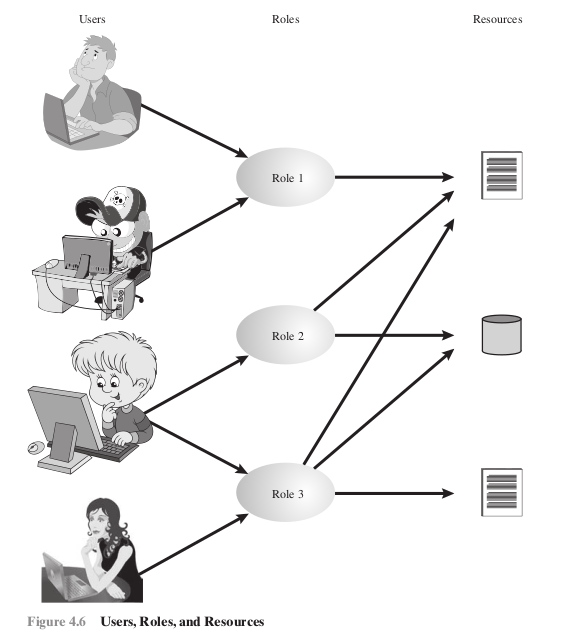
\includegraphics[width=14cm, keepaspectratio]{Bistarelli/img/cap_4/figura4.6.png}
\end{figure}

\begin{figure}[H]
	\centering
    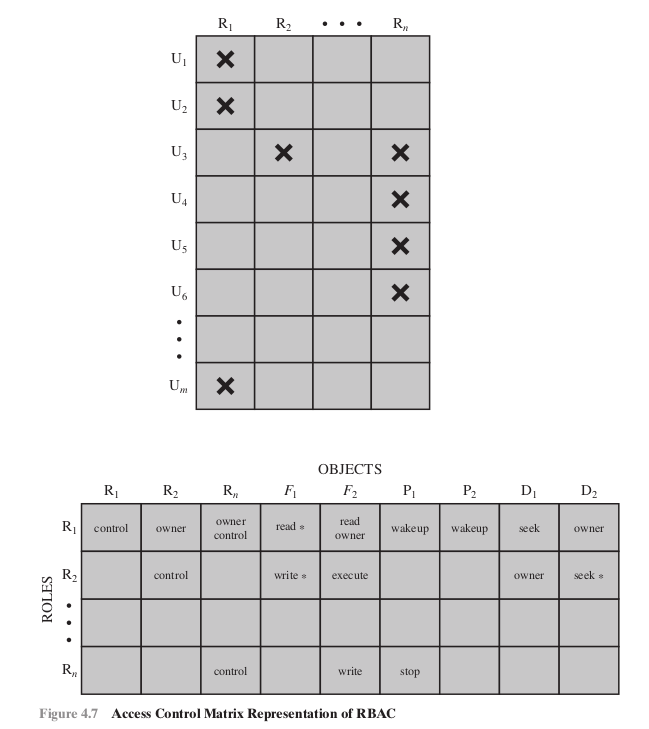
\includegraphics[width=14cm, keepaspectratio]{Bistarelli/img/cap_4/figura4.7.png}
\end{figure}


I sistemi DAC tradizionali definiscono i diritti di accesso dei singoli utenti e dei gruppi di utenti. Al contrario, RBAC si basa sui ruoli che gli utenti assumono in un sistema piuttosto che sull'identità dell'utente. Tipicamente, i modelli RBAC definiscono un ruolo come una funzione lavorativa all'interno un'organizzazione. I sistemi RBAC assegnano i diritti di accesso ai ruoli invece che ai singoli utenti. A loro volta, gli utenti sono assegnati a diversi ruoli, sia staticamente che dinamicamente, secondo le loro responsabilità.

\singlespacing

RBAC ora gode di un ampio uso commerciale e rimane un'area di ricerca attiva. Il National Institute of Standards and Technology (NIST) ha emesso uno standard, FIPS PUB 140-3 (Security Requirements for Cryptographic Modules, settembre 2009), che richiede il supporto per il controllo degli accessi e l'amministrazione attraverso i ruoli. La relazione degli utenti con i ruoli è molti a molti, così come la relazione dei ruoli alle risorse o agli oggetti del sistema (vedi Figura 4.6). L'insieme degli utenti cambia, in alcuni ambienti frequentemente, e l'assegnazione di un utente a uno o più ruoli può anche essere dinamico. L'insieme dei ruoli nel sistema nella maggior parte degli ambienti è relativamente statico, con solo occasionali aggiunte o cancellazioni. Ogni ruolo avrà diritti di accesso specifici a una o più risorse. L'insieme delle risorse e i diritti di accesso specifici associati con un particolare ruolo è probabile che cambino raramente.

\singlespacing

Possiamo usare la rappresentazione della matrice di accesso per rappresentare gli elementi chiave di un sistema RBAC in termini semplici, come mostrato nella figura 4.7. La matrice superiore mette in relazione i singoli utenti ai ruoli. Tipicamente ci sono molti più utenti che ruoli. Ogni matrice voce della matrice è vuota o marcata, quest'ultima indica che l'utente è assegnato a questo ruolo. Si noti che un singolo utente può essere assegnato a più ruoli (più di un segno in una riga) e più utenti possono essere assegnati a un singolo ruolo (più di un segno in una colonna). La matrice inferiore ha la stessa struttura della matrice di controllo degli accessi DAC, con i ruoli come soggetti. Tipicamente, ci sono pochi ruoli e molti oggetti, o risorse. In questa matrice, le voci sono i diritti di accesso specifici dei ruoli. Si noti che un ruolo può essere trattato come un oggetto, permettendo la definizione di gerarchie di ruoli.

\singlespacing

\textbf{RBAC} si presta ad un'efficace implementazione del principio del minimo privilegio, a cui si fa riferimento nel capitolo 1. Ogni ruolo dovrebbe contenere l'insieme minimo di diritti di accesso necessari per quel ruolo. Un utente viene assegnato ad un ruolo che gli permette di eseguire solo ciò che è richiesto per quel ruolo. Più utenti assegnati allo stesso ruolo godono dello stesso insieme minimo di diritti di accesso.
\newpage
\subsection{Modelli di riferimento RBAC}

\begin{figure}[H]
	\centering
    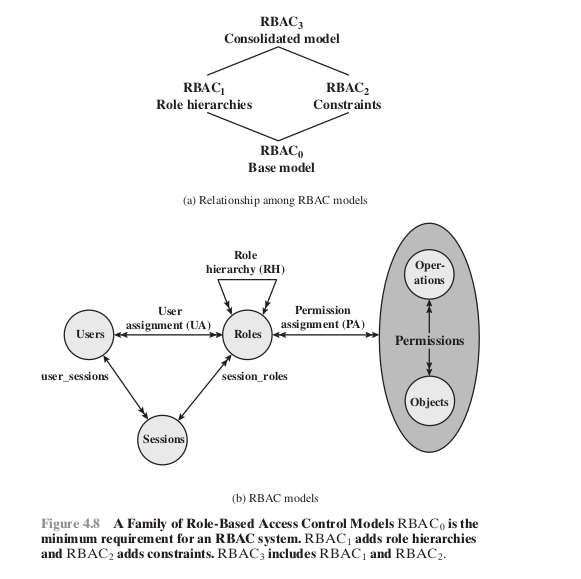
\includegraphics[width=14cm, keepaspectratio]{Bistarelli/img/cap_4/figura4.8.png}
\end{figure}

\begin{figure}[H]
	\centering
    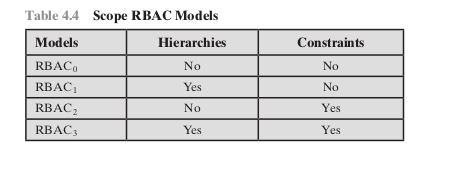
\includegraphics[width=14cm, keepaspectratio]{Bistarelli/img/cap_4/tabella4.4.png}
\end{figure}

Una varietà di funzioni e servizi possono essere inclusi sotto l'approccio generale RBAC approccio. Per chiarire i vari aspetti di RBAC, è utile definire un insieme di modelli astratti modelli astratti di funzionalità RBAC.

\singlespacing

Definisce una famiglia di modelli di riferimento che è servita come base per gli sforzi di standardizzazione in corso. Questa famiglia consiste di quattro modelli che sono correlati tra loro, come mostrato nella Figura 4.8a e nella Tabella 4.4. RBAC 0 contiene la funzionalità minima per un sistema RBAC.

\singlespacing

RBAC 1 include le funzionalità di RBAC 0 e aggiunge le gerarchie dei ruoli, che permettono a un ruolo di ereditare i permessi da un altro ruolo. RBAC 2 include RBAC 0 e aggiunge vincoli, che limitano i modi in cui i componenti di un sistema RBAC possono essere configurati. RBAC 3 contiene la funzionalità di RBAC 0, RBAC1 e RBAC2.

\singlespacing

\paragraph{Modello base-RBAC0}

Figura 4.8b, senza la gerarchia dei ruoli e i vincoli, contiene i quattro tipi di entità in un sistema RBAC 0:
\begin{itemize}

    \item \textbf{Utente:} un individuo che ha accesso a questo sistema informatico. Ogni individuo ha un ID utente associato.
    
    \item \textbf{Ruolo:} Una funzione di lavoro nominata all'interno dell'organizzazione che controlla questo sistema informatico. Tipicamente, associato ad ogni ruolo c'è una descrizione dell'autorità e della responsabilità conferite a questo ruolo, e a qualsiasi utente che assume questo ruolo.
    
    \item \textbf{Permesso:} Un'approvazione di una particolare modalità di accesso a uno o più oggetti. Termini equivalenti sono diritto di accesso, privilegio e autorizzazione.
    
    \item \textbf{Sessione:} Una mappatura tra un utente e un sottoinsieme attivato dell'insieme di ruoli a cui l'utente è assegnato.
    
\end{itemize}

Le linee con le frecce nella figura 4.8b indicano relazioni, o mappature, con una freccia singola che ne indica una e una doppia che ne indica molte. Quindi, c'è una relazione molti-a-molti tra utenti e ruoli: Un utente può avere più ruoli, e più utenti possono essere assegnati a un singolo ruolo. Allo stesso modo, c'è una relazione molti a molti tra ruoli e permessi. Una sessione è usata per definire una relazione temporanea uno-a-molti tra un utente e uno o più ruoli a cui l'utente è stato assegnato. L'utente stabilisce una sessione con solo i ruoli necessari per un particolare compito; questo è un esempio del concetto di minimo privilegio. Le relazioni molti-a-molti tra utenti e ruoli e tra ruoli e permessi forniscono una flessibilità e granularità di assegnazione che non si trova negli schemi DAC convenzionali. Senza questa flessibilità e granularità, c'è un rischio maggiore che ad un utente possa essere concesso più accesso alle risorse di quanto sia necessario a causa del controllo limitato sui tipi di accesso che possono essere permessi. 
\newpage
\begin{center}
    \textbf{Gerarchie di ruolo-RBAC1}
\end{center}

Le gerarchie di ruolo forniscono un mezzo per riflettere la struttura gerarchica dei ruoli in un'organizzazione. Tipicamente, le funzioni lavorative con maggiore responsabilità hanno maggiore autorità per accedere alle risorse. Una funzione lavorativa subordinata può avere un sottoinsieme dei diritti di accesso della funzione lavorativa superiore. Le gerarchie di ruolo fanno uso del concetto di ereditarietà per permettere ad un ruolo di includere implicitamente i diritti di accesso associati ad un ruolo subordinato. La figura 4.9 è un esempio di diagramma di una gerarchia di ruoli. Per convenzione, i ruoli subordinati sono più in basso nel diagramma. Una linea tra due ruoli implica che il ruolo superiore include tutti i diritti di accesso del ruolo inferiore, così come altri diritti di accesso non disponibili al ruolo inferiore. Un ruolo può ereditare diritti di accesso da più ruoli subordinati. Per esempio, nella figura 4.9, il ruolo Project Lead include tutti i diritti di accesso del ruolo Production Engineer e del ruolo Quality Engineer. Più di un ruolo può ereditare dallo stesso ruolo subordinato. Per esempio, sia il ruolo Production Engineer che il ruolo Quality Engineer includono tutti i diritti di accesso del ruolo Engineer. Ulteriori diritti di accesso sono anche assegnati al ruolo Production Engineer, e un diverso insieme di diritti di accesso aggiuntivi sono assegnati al ruolo Quality ingegnere di qualità. Quindi, questi due ruoli hanno diritti di accesso che si sovrappongono, vale a dire i diritti di accesso diritti di accesso che condividono con il ruolo Engineer.

\begin{center}
    \textbf{Vincoli-RBAC2}
\end{center}

I vincoli forniscono un mezzo per adattare RBAC alle specifiche delle politiche amministrative e di sicurezza in un'organizzazione. Un vincolo è una relazione definita tra i ruoli o una condizione relativa ai ruoli. Esistono i seguenti tipi di vincoli: ruoli mutuamente esclusivi, cardinalità e ruoli prerequisiti. I ruoli mutuamente esclusivi sono ruoli tali che un utente può essere assegnato ad un solo ruolo nell'insieme. Questa limitazione potrebbe essere statica, o potrebbe essere dinamica, nel senso che ad un utente potrebbe essere assegnato solo uno dei ruoli nell'insieme per una sessione. Il vincolo reciprocamente esclusivo supporta una separazione di doveri e capacità all'interno un'organizzazione. Questa separazione può essere rafforzata o migliorata dall'uso di assegnazioni di permessi reciprocamente esclusivi. Con questo vincolo aggiuntivo, un insieme di ruoli mutuamente esclusivi ha le seguenti proprietà:

\begin{center}
    Un utente può essere assegnato ad un solo ruolo nell'insieme (sia durante una sessione staticamente).
Qualsiasi permesso (diritto di accesso) può essere concesso ad un solo ruolo dell'insieme.
\end{center}

\begin{figure}[H]
	\centering
    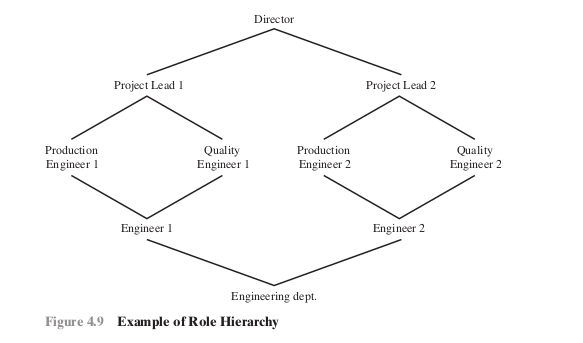
\includegraphics[width=14cm, keepaspectratio]{Bistarelli/img/cap_4/figura4.9.png}
\end{figure}


\singlespacing

Così, l'insieme dei ruoli reciprocamente esclusivi hanno permessi non sovrapposti. Se due utenti sono assegnati a ruoli diversi nell'insieme, allora gli utenti hanno permessi non sovrapposti permessi mentre assumono quei ruoli. Lo scopo dei ruoli mutuamente esclusivi è quello di aumentare la difficoltà di collusione tra individui con competenze diverse o funzioni funzioni lavorative divergenti per contrastare le politiche di sicurezza. La cardinalità si riferisce all'impostazione di un numero massimo rispetto ai ruoli. Uno di questi vincolo è quello di impostare un numero massimo di utenti che possono essere assegnati ad un dato ruolo.

Per esempio, un ruolo di capo progetto o un ruolo di capo reparto potrebbe essere limitato ad un singolo utente. Il sistema potrebbe anche imporre un vincolo sul numero di ruoli che un utente è assegnato, o il numero di ruoli che un utente può attivare per una singola sessione. Un'altra forma di vincolo è quella di impostare un numero massimo di ruoli che possono essere concessi un particolare permesso; questa potrebbe essere una tecnica desiderabile di mitigazione del rischio per un permesso sensitiva o potente.

\singlespacing

Un sistema potrebbe essere in grado di specificare un ruolo prerequisito, che impone che un utente possa essere assegnato a un particolare ruolo solo se è già assegnato a qualche altro ruolo specificato.

\singlespacing

Un prerequisito può essere usato per strutturare l'implementazione del concetto di minimo privilegio. In una gerarchia, potrebbe essere richiesto che un utente possa essere assegnato ad un ruolo (superiore) solo se gli è già stato assegnato un ruolo immediatamente inferiore. Per esempio, nella figura 4.9 un utente assegnato a un ruolo di Project Lead deve essere assegnato anche a ai ruoli subordinati Production Engineer e Quality Engineer. Quindi, se l'utente non ha bisogno di tutti i permessi del ruolo Project Lead per un dato compito, l'utente può invocare una sessione usando solo il ruolo subordinato richiesto. Si noti l'uso di prerequisiti legati al concetto di gerarchia richiede il modello RBAC 3.
\section{Controllo degli accessi basato su attributi}
Uno sviluppo relativamente recente nella tecnologia di controllo dell'accesso è il modello di controllo dell'accesso basato sugli attributi (ABAC). Un modello ABAC può definire autorizzazioni che esprimono condizioni su proprietà sia della risorsa che del soggetto. Per esempio, consideriamo una configurazione in cui ogni risorsa ha un attributo che identifica il soggetto che ha creato la risorsa. Quindi, una singola regola di accesso può specificare il privilegio del proprietario per tutti i creatori di ogni risorsa. La forza dell'approccio ABAC è la sua flessibilità e potenza espressiva. Sottolinea che il principale ostacolo alla sua adozione in sistemi reali è stata la preoccupazione per l'impatto della valutazione dei predicati su entrambe le proprietà della risorsa e dell'utente per ogni accesso.
\singlespacing
Tuttavia, per applicazioni come i servizi Web cooperanti e il cloud computing questo aumento del costo delle prestazioni è meno evidente perché c'è già un costo di prestazione relativamente alto per ogni accesso. Così, i servizi Web sono stati tecnologie innovative per l'implementazione di modelli ABAC, specialmente attraverso l'introduzione dell'eXtensible Access Control Markup Language (XAMCL) e c'è un notevole interesse nell'applicare il modello ABAC ai servizi cloud.
\singlespacing
Ci sono tre elementi chiave in un modello ABAC: gli attributi, che sono definiti per le entità in una configurazione; un modello di policy, che definisce le politiche ABAC; e il modello di architettura, che si applica alle politiche che impongono il controllo degli accessi.
\newpage
\subsection{Attributi}
Gli attributi sono caratteristiche che definiscono aspetti specifici del soggetto, dell'oggetto, delle condizioni ambientali e/o delle operazioni richieste che sono predefinite e preassegnate da un'autorità. Gli attributi contengono informazioni che indicano la classe di informa un nome e un valore (ad esempio, Class = HospitalRecordsAccess, Name = PatientInformationAccess, Value = MFBusinessHoursOnly).
\singlespacing
I seguenti sono i tre tipi di attributi nel modello ABAC:
\begin{itemize}
    \item \textbf{Attributi soggetto}
    
Un soggetto è un'entità attiva (ad esempio, un utente, un'applicazione, un processo o un dispositivo) che causa il flusso di informazioni tra gli oggetti o cambia lo stato del sistema. Ogni soggetto ha degli attributi associati che definiscono l'identità e le caratteristiche del soggetto. Tali attributi possono includere l'identificatore del soggetto identificatore, nome, organizzazione, titolo di lavoro e così via. Anche il ruolo di un soggetto può essere visto come un attributo.

    \item \textbf{Attributi dell'oggetto}
    
Un oggetto, chiamato anche risorsa, è un oggetto passivo (nel contesto della richiesta data) un'entità legata al sistema informativo (ad esempio, dispositivi, file, record, tabelle, processi, programmi, reti, domini) che contengono o ricevere informazioni. Come per i soggetti, gli oggetti hanno attributi che possono essere per prendere decisioni di controllo dell'accesso.

    \item \textbf{Attributi ambientali}
    
Questi attributi sono stati finora largamente ignorati nella maggior parte delle politiche di controllo degli accessi. Essi descrivono l'ambiente operativo, tecnico e anche ambiente o contesto situazionale in cui avviene l'accesso alle informazioni. Per esempio, attributi come la data e l'ora correnti, le attività correnti di virus/hacker e il livello di sicurezza della rete (ad esempio, Internet o intranet), non sono associati ad un particolare soggetto o ad una risorsa, ma possono comunque essere rilevanti nell'applicazione di una politica di controllo degli accessi. ABAC è un modello di controllo dell'accesso logico che si distingue perché controlla l'accesso agli oggetti valutando le regole contro gli attributi delle entità (soggetto e oggetto), le operazioni e oggetto), delle operazioni e dell'ambiente rilevanti per una richiesta. ABAC si basa sulla valutazione degli attributi del soggetto, degli attributi dell'oggetto e di una relazione forzata o una regola di controllo dell'accesso che definisce le operazioni consentite per le combinazioni di attributi di soggetto e oggetto in un dato ambiente.
\end{itemize}

\singlespacing

Tutte le soluzioni ABAC contengono queste capacità di base per valutare gli attributi e applicare regole o relazioni tra questi attributi. I sistemi ABAC sono in grado di applicare i concetti DAC, RBAC e concetti MAC. ABAC consente un controllo dell'accesso a grana fine, che permette un numero numero di input discreti in una decisione di controllo dell'accesso, fornendo un più grande insieme di possibili combinazioni di quelle variabili per riflettere un insieme più ampio e definitivo di possibili regole, politiche o restrizioni di accesso. Così, ABAC permette un numero illimitato numero illimitato di attributi da combinare per soddisfare qualsiasi regola di controllo dell'accesso. Inoltre, i sistemi ABAC possono essere implementati per soddisfare una vasta gamma di requisiti da dalle liste di controllo degli accessi di base a modelli di policy avanzati ed espressivi che sfruttano appieno la flessibilità dell'ABAC.
\newpage
\subsection{Architettura locìgica ABAC}
\begin{figure}[H]
	\centering
    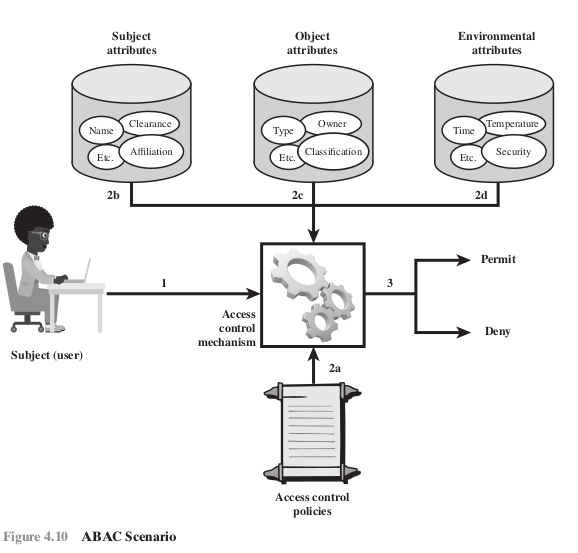
\includegraphics[width=14cm, keepaspectratio]{Bistarelli/img/cap_4/figura4.10.png}
\end{figure}

La figura 4.10 illustra in un'architettura logica i componenti essenziali di un sistema ABAC.

\singlespacing

Un accesso di un soggetto a un oggetto procede secondo i seguenti passi:

\begin{enumerate}

    \item Un soggetto richiede l'accesso ad un oggetto. Questa richiesta viene inoltrata ad un meccanismo di controllo meccanismo di controllo dell'accesso.
    
    \item Il meccanismo di controllo degli accessi è governato da un insieme di regole (2a) che sono definite da una politica di controllo dell'accesso preconfigurata. Sulla base di queste regole, il meccanismo di controllo dell'accesso valuta gli attributi del soggetto (2b), dell'oggetto (2c) e le condizioni ambientali (2d) per determinare l'autorizzazione.
    
    \item Il meccanismo di controllo dell'accesso concede al soggetto l'accesso all'oggetto se l'accesso è autorizzato, e nega l'accesso se non è autorizzato. È chiaro dall'architettura logica che ci sono quattro fonti indipendenti di informazioni utilizzate per la decisione di controllo dell'accesso.

\end{enumerate}

Il progettista del sistema può decidere quali attributi sono importanti per il controllo dell'accesso rispetto a soggetti, oggetti e condizioni ambientali. Il progettista del sistema o altra autorità può quindi definire politiche di controllo dell'accesso, sotto forma di regole, per qualsiasi combinazione desiderata di attri di soggetti, oggetti e condizioni ambientali.

\singlespacing

Dovrebbe essere evidente che questo approccio è molto potente e flessibile. Tuttavia, il costo, sia in termini di complessità della progettazione e dell'implementazione, e in termini di impatto sulle prestazioni, è probabile che superi quello di altri approcci di controllo dell'accesso. Questo è un compromesso che autorità di sistema deve fare.

\singlespacing

Rispetto a un modello DAC che usa liste di controllo degli accessi (ACL). Questa figura non solo illustra la complessità relativa dei due modelli, ma chiarisce anche i requisiti di fiducia dei due modelli. Un confronto delle relazioni di fiducia rappresentative (indicate dalle linee con la freccia) per l'uso di ACL e ABAC mostra che ci sono molte relazioni di fiducia più complesse richieste per ABAC per funzionare correttamente. Ignorando i punti in comune in entrambe le parti della Figura 4.11, si può osservare che con le ACL la radice della fiducia è con il proprietario dell'oggetto, il quale applica in che fa rispettare le regole di accesso all'oggetto fornendo l'accesso all'oggetto attraverso l'aggiunta di un utente ad una ACL.

\singlespacing

L'aggiunta di un utente ad una ACL. In ABAC, la radice della fiducia deriva da molte fonti di cui il proprietario dell'oggetto non ha controllo, come le Subject Attribute Authorities, sviluppatori di policy e emittenti di credenziali. Di conseguenza, SP 800-162 raccomandava che un organismo di governance aziendale sia formato per gestire tutte le identità, le credenziali, di gestione delle identità, delle credenziali e degli accessi e che ogni organizzazione sub-ordinata mantenga un organismo simile per garantire la coerenza nella gestione l'implementazione e il cambiamento di paradigma associati all'implementazione di ABAC a livello aziendale.

\singlespacing

Inoltre, si raccomanda che un'impresa sviluppi un modello di fiducia che può essere usato per illustrare le relazioni di fiducia e aiutare a determinare la proprietà e la responsabilità delle informazioni e dei servizi, le esigenze di ulteriori politiche e di governance e i requisiti per soluzioni tecniche per convalidare o applicare le relazioni di fiducia. Il modello di fiducia di modello di fiducia può essere usato per influenzare le organizzazioni a condividere le loro informazioni con chiare aspettative su come queste informazioni saranno usate e protette e per essere in grado di fidarsi delle informazioni e delle asserzioni di attributi e autorizzazioni provenienti da altre organizzazioni.

\subsection{Politiche ABAC}
Una politica è un insieme di regole e relazioni che governano il comportamento consentito all'interno di un'organizzazione. Basato sui privilegi dei soggetti e su come le risorse o gli oggetti devono essere protetti in quali condizioni ambientali. A loro volta, i privilegi rappresentano il comportamento autorizzato di un soggetto; sono definiti da un'autorità e incorporati in una politica. Altri termini comunemente usati al posto di privilegi sono autorizzazioni e diritti. La politica è tipicamente scritta dal punto di vista dell'oggetto da proteggere e dei privilegi disponibili ai soggetti. Ora definiamo un modello di policy ABAC. Sono utilizzate le seguenti convenzioni


S, O ed E sono rispettivamente soggetti, oggetti e ambienti

SAk (1 <= k <= K), OAm (1 <= m <= M), e EAn (1 <= n <= N) sono gli attributi predefiniti per soggetti, oggetti e ambienti, rispettivamente

\begin{figure}[H]
	\centering
    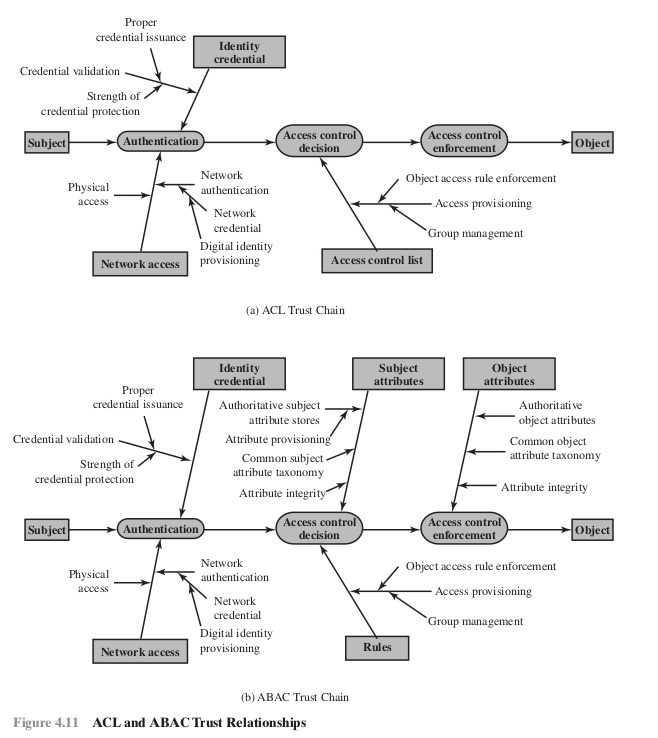
\includegraphics[width=12cm, keepaspectratio]{Bistarelli/img/cap_4/figura4.11.png}
\end{figure}

ATTR(s), ATTR(o), e ATTR(e) sono relazioni di assegnazione di attributi per il soggetto s, oggetto o, e ambiente e, rispettivamente:

\begin{figure}[H]
	\centering
    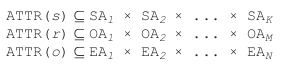
\includegraphics[width=10cm, keepaspectratio]{Bistarelli/img/cap_4/figura4.png}
\end{figure}

Usiamo anche la notazione di funzione per l'assegnazione del valore dei singoli attributi. Per esempio:

\begin{figure}[H]
	\centering
    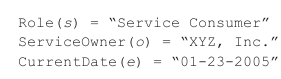
\includegraphics[width=10cm, keepaspectratio]{Bistarelli/img/cap_4/figura4-2.png}
\end{figure}

Nella forma più generale, una Policy Rule, che decide se un soggetto s può accedere ad un oggetto o in un particolare ambiente e, è una funzione booleana degli attributi di s, o ed e:
Inserire immagine

Una base di regole di policy o policy store può consistere in un certo numero di regole di policy, che coprono molti soggetti e oggetti all'interno di un dominio di sicurezza. Il controllo dell'accesso Il processo decisionale del controllo d'accesso equivale essenzialmente alla valutazione delle regole di nell'archivio delle politiche.

Ora considerate l'esempio di un negozio di intrattenimento online che trasmette film agli utenti per una tariffa mensile fissa. Useremo questo esempio per contrastare gli approcci RBAC e ABAC approcci. Il negozio deve applicare la seguente politica di controllo degli accessi basata sull'età all'età dell'utente e alla classificazione del contenuto del film:

\begin{figure}[H]
	\centering
    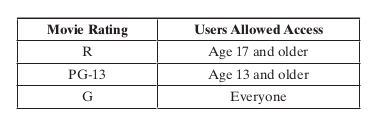
\includegraphics[width=10cm, keepaspectratio]{Bistarelli/img/cap_4/tabella4.png}
\end{figure}

In un modello RBAC, ad ogni utente verrebbe assegnato uno dei tre ruoli: Adulto, Juvenile, o Child, possibilmente durante la registrazione. Ci sarebbero tre permessi creati: Può vedere film vietati ai minori, Può vedere film vietati ai minori, e Può vedere i film vietati ai minori. Il ruolo Adulto viene assegnato con tutti e tre i permessi.

Il ruolo Juvenile ottiene le autorizzazioni Can view PG-13-rated movies e Can view G-rated movies e il ruolo Bambino ottiene solo il permesso di visualizzare i film vietati ai minori.

Entrambe le assegnazioni utente-ruolo e permesso-ruolo sono compiti amministrativi manuali. L'approccio ABAC a questa applicazione non ha bisogno di definire esplicitamente i ruoli. Invece, se un utente u può accedere o vedere un film m (in un ambiente di sicurezza e che qui viene ignorato) verrebbe risolto valutando una regola di policy come la seguente:

\begin{figure}[H]
	\centering
    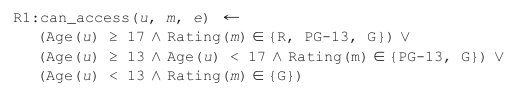
\includegraphics[width=11cm, keepaspectratio]{Bistarelli/img/cap_4/formula.png}
\end{figure}

dove Age e Rating sono rispettivamente l'attributo soggetto e l'attributo oggetto. Il vantaggio del modello ABAC mostrato qui è che elimina la definizione e la gestione di ruoli statici, eliminando così la necessità di compiti amministrativi per l'assegnazione da utente a ruolo e da permesso a ruolo.

Il vantaggio di ABAC si vede più chiaramente quando imponiamo politiche a grana più fine. Per esempio, supponiamo che i film siano classificati come New Release o Old Release, in base alla data di rilascio rispetto alla data corrente, e che gli utenti siano classificati come classificati come Utente Premium e Utente Regolare, in base alla tariffa che pagano. Vorremmo applicare una politica per cui solo gli utenti premium possono vedere i nuovi film. Per il modello RBAC, dovremmo raddoppiare il numero di ruoli, per distinguere ogni utente per età e tariffa, e dovremmo raddoppiare il numero di permessi separati pure.

In generale, se ci sono K attributi soggetto e M attributi oggetto, e se per ogni attributo, Range() denota l'intervallo di valori possibili che può assumere, allora il rispettivo numero di ruoli e permessi richiesti per un modello RBAC sono:

\begin{figure}[H]
	\centering
    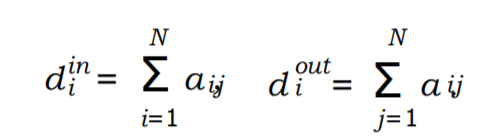
\includegraphics[width=11cm, keepaspectratio]{Bistarelli/img/cap_4/formula2.png}
\end{figure}

Così, possiamo vedere che quando il numero di attributi aumenta per ospitare politiche a grana più fine, il numero di ruoli e permessi cresce esponenzialmente.

Al contrario, il modello ABAC tratta gli attributi aggiuntivi in modo efficiente. Per questo esempio, la policy R1 definita in precedenza è ancora valida. Abbiamo bisogno di due nuove regole:

\begin{figure}[H]
	\centering
    \includegraphics[width=12cm, keepaspectratio]{Bistarelli/img/cap_4/foto4-3.png}
\end{figure}

Con il modello ABAC, è anche facile aggiungere attributi ambientali. Supponiamo che che vogliamo aggiungere una nuova regola di policy che è espressa in parole come segue: Gli utenti regolari sono autorizzati a vedere le nuove release nei periodi promozionali. Questo sarebbe difficile da esprimere in un modello RBAC. In un modello ABAC, abbiamo solo bisogno di aggiungere una regola congiuntiva (AND) che controlla per vedere se l'attributo ambientale la data di oggi cade in un periodo promozionale.
\newpage
\section{Gestione dell'entità, delle credenziali e dell'accesso}
L'ICAM è un approccio completo alla gestione e all'implementazione delle identità digitali identità digitali (e gli attributi associati), le credenziali e il controllo degli accessi. ICAM è stato sviluppato dal governo degli Stati Uniti, ma è applicabile non solo alle agenzie governative, ma può anche essere distribuito da imprese che cercano un approccio unificato al controllo degli accessi. ICAM è progettato per:
\begin{itemize}

    \item Creare rappresentazioni fidate di identità digitali di individui e di ciò che i documenti ICAM si riferiscono a entità non personali (NPE). Queste ultime includono processi, applicazioni e dispositivi automatici che cercano di accedere a una risorsa.
    
    \item Legare queste identità a credenziali che possono servire come proxy per l'individuo o NPE nelle transazioni di accesso. Una credenziale è un oggetto o una struttura di dati che lega autorevolmente un'identità (e opzionalmente, attributi aggiuntivi) a un token posseduto e controllato da un sottoscrittore.
    
    \item Utilizza le credenziali per fornire un accesso autorizzato alle risorse di un'agenzia.
\end{itemize}
\newpage
\subsection{Gestione dell'identità}
La gestione dell'identità si occupa di assegnare attributi a un'identità digitale e di collegare tale identità digitale a un individuo o a una NPE. L'obiettivo è quello di stabilire un'identità digitale affidabile che sia indipendente da una specifica applicazione o contesto.

\singlespacing

L'approccio tradizionale, e ancora più comune, al controllo dell'accesso per applicazioni e programmi è quello di creare una rappresentazione digitale di un'identità per l'uso specifico di l'applicazione o il programma. Di conseguenza, il mantenimento e la protezione dell'identità stessa è trattata come secondaria rispetto alla missione associata all'applicazione. Inoltre, c'è una considerevole sovrapposizione di sforzi nello stabilire queste identità specifiche dell'applicazione.

\singlespacing

A differenza degli account usati per accedere a reti, sistemi o applicazioni, i record di identità aziendali non sono legati al titolo di lavoro, alle mansioni lavorative, all'ubicazione o al fatto che sia necessario l'accesso a un sistema specifico. Questi elementi possono diventare attributi legati ad un record di identità e possono anche diventare parte di ciò che identifica in modo univoco un individuo in una specifica applicazione. Le decisioni sul controllo degli accessi saranno basate sul contesto e sugli attributi rilevanti di un utente non solo sulla sua identità. Il concetto di un'identità aziendale è che gli individui avranno una singola rappresentazione digitale di se stessi che può essere sfruttata in tutti i dipartimenti e le agenzie per molteplici scopi, compreso il controllo degli accessi.

\singlespacing

\begin{figure}[H]
	\centering
    \includegraphics[width=10cm, keepaspectratio]{Bistarelli/img/cap_4/figura4.12.png}
\end{figure}

La figura 4.12 illustra le funzioni chiave coinvolte nella gestione delle identità. Un'identità digitale inizia tipicamente con la raccolta di dati di identità come parte di un processo di iscrizione. Un'identità digitale è spesso composta da un insieme di attributi che aggregati identificano in modo univoco un utente all'interno di un sistema o di un'azienda. Al fine di stabilire la fiducia nell'individuo rappresentato da un'identità digitale, un'agenzia può anche condurre un'indagine di fondo.

\singlespacing

Gli attributi di un individuo possono essere memorizzati in varie fonti autorevoli all'interno di un'agenzia e collegati per formare una visione aziendale dell'identità digitale. Questa identità digitale può quindi essere fornita in applicazioni per supportare l'accesso fisico e logico (parte della gestione degli accessi) e de-provisionata quando l'accesso non è più richiesto.

\singlespacing

Un elemento finale della gestione delle identità è la gestione del ciclo di vita, include quanto segue:

\begin{itemize}
    \item Meccanismi, politiche e procedure per proteggere l'identità personale informazioni
    
    \item Controllo dell'accesso ai dati di identità
    
    \item Tecniche per condividere dati di identità autorevoli con le applicazioni che ne hanno bisogno

    \item Revoca di un'identità aziendale
\end{itemize}
\newpage
\subsection{Gestione delle credenziali}
Come detto, una credenziale è un oggetto o una struttura di dati che lega autorevolmente un'identità (e opzionalmente, attributi aggiuntivi) ad un token posseduto e controllato da un sottoscrittore. Esempi di credenziali sono le smart card, le chiavi crittografiche private/pubbliche crittografiche private/pubbliche e i certificati digitali. La gestione delle credenziali è la gestione del ciclo di vita ciclo di vita della credenziale.
\singlespacing
La gestione delle credenziali comprende i seguenti cinque componenti logistici:
\begin{enumerate}
    \item Un individuo autorizzato sponsorizza un individuo o un'entità per una credenziale per stabilire la necessità della credenziale. Per esempio, un supervisore di reparto sponsorizza un dipendente del dipartimento.

    \item L'individuo sponsorizzato si iscrive per la credenziale, un processo che tipicamente consiste in una prova d'identità e nella cattura di dati biografici e di dati di sicurezza.

un processo che tipicamente consiste nella prova dell'identità e nell'acquisizione di dati biografici e biometrici. Questo passo può anche comportare l'incorporazione di dati di attributo autorevoli, mantenuti dal dal componente di gestione dell'identità.

    \item Viene prodotta una credenziale. A seconda del tipo di credenziale, la produzione può coinvolgere la crittografia, l'uso di una firma digitale, la produzione di una smartcard, o altre funzioni.

    \item La credenziale viene rilasciata all'individuo o alla NPE.
    
    \item Una credenziale deve essere mantenuta durante il suo ciclo di vita, che potrebbe includere la revoca, la riemissione/sostituzione, la reiscrizione, la scadenza, la reimpostazione del numero di identificazione personale (PIN), sospensione o reintegrazione.
\end{enumerate}
\newpage
\subsection{Gestione degli accessi}
Il componente di gestione degli accessi si occupa della gestione e del controllo delle modalità di accesso alle risorse da parte delle entità. Copre sia l'accesso logico che fisiologico e può essere interno ad un sistema o un elemento esterno. Lo scopo della gestione degli accessi è quello di garantire che venga fatta la corretta verifica dell'identità quando un individuo tenta di accedere a edifici, sistemi informatici o dati sensibili alla sicurezza. La funzione di controllo degli accessi fa uso delle credenziali presentate da chi richiede l'accesso e l'identità digitale del richiedente.
\singlespacing
Sono necessari tre elementi di supporto per una struttura di controllo degli accessi a livello aziendale:
\begin{itemize}
    \item \textbf{Gestione delle risorse}
    
Questo elemento riguarda la definizione di regole per una risorsa che richiede il controllo dell'accesso. Le regole includeranno le credenziali requisiti delle credenziali e quali attributi dell'utente, attributi della risorsa e condizioni ambientali sono richieste per l'accesso ad una data risorsa per una data funzione.

\item \textbf{Gestione dei privilegi}

Questo elemento si occupa di stabilire e mantenere di diritti o attributi di privilegio che comprendono il profilo di accesso di un individuo. Questi attributi rappresentano caratteristiche di un individuo che possono essere utilizzati come base per determinare le decisioni di accesso alle risorse fisiche e logiche. I privilegi sono considerati attributi che possono essere collegati a un'identità digitale. identità digitale.

\item \textbf{Gestione delle politiche}

Questo elemento governa ciò che è permesso e non permesso in una transazione di accesso. Cioè, dati l'identità e gli attributi del richiedente, gli attributi della risorsa o dell'oggetto e le condizioni ambientali, una politica specifica quali azioni questo utente può eseguire su questo oggetto.
\end{itemize}
\newpage
\subsection{Federazione delle identità}
La federazione di identità affronta due questioni:
\begin{enumerate}
    \item Come vi fidate delle identità di individui di organizzazioni esterne che hanno bisogno di accesso ai vostri sistemi?
    
    \item Come garantisci le identità degli individui della tua organizzazione quando hanno hanno bisogno di collaborare con organizzazioni esterne?
\end{enumerate}
La federazione delle identità è un termine usato per descrivere la tecnologia, gli standard, le politiche e processi che permettono a un'organizzazione di fidarsi di identità digitali, attributi di identità e credenziali create ed emesse da un'altra organizzazione.
\section{Strutte di fiducia}
I concetti interconnessi di fiducia, identità e attributi sono diventati preoccupazioni fondamentali delle imprese Internet, dei fornitori di servizi di rete e delle grandi imprese. Queste preoccupazioni possono essere viste chiaramente nell'ambiente del commercio elettronico. Per l'efficienza, la privacy e la semplicità legale, le parti delle transazioni generalmente applicano il principio del need-to-know: cosa si deve sapere di qualcuno per trattare con lui? La risposta varia da caso a caso, e include attributi come il numero di registrazione professionale o di licenza, l'organizzazione e il dipartimento, l'ID del personale, il nulla osta di sicurezza, il numero di riferimento del cliente, il numero di carta di credito, l'identificatore unico della salute, le allergie, il gruppo sanguigno, il numero di previdenza sociale, l'indirizzo, lo stato di cittadino, il nickname dei social network, lo pseudonimo e così via. Gli attributi di un individuo che devono essere conosciuti e verificati per permettere una transazione dipendono dal contesto. Per esempio, un'impresa può bisogno di fornire accesso alle risorse per clienti, utenti, fornitori e partner. A seconda del contesto, l'accesso sarà determinato non solo dall'identità, ma dagli attributi del richiedente e della risorsa.
\newpage
\subsection{Approccio tradizionale allo scambio di identità}
Le transazioni online o in rete che coinvolgono parti di diverse organizzazioni, o tra un'organizzazione e un utente individuale come un cliente online, richiedono generalmente la condivisione di informazioni di identità. Queste informazioni possono includere una serie di attributi associati oltre a un semplice nome o identificatore numerico. Sia la parte che divulga le informazioni che quella che le riceve devono avere un livello di fiducia sulle questioni di sicurezza e di privacy relative a tali informazioni. La figura 4.13a mostra la tecnica tradizionale per lo scambio di informazioni sull'identità. Questo comporta che gli utenti sviluppino accordi con un fornitore di servizi di identità per procurarsi identità e credenziali digitali, e accordi con le parti che forniscono servizi e applicazioni per gli utenti finali e che sono disposti a fare affidamento sull'identità e sulle informazioni sull'identità e le credenziali generate dal fornitore di servizi d'identità. L'accordo della Figura 4.13a deve soddisfare una serie di requisiti. La parte fidata richiede che l'utente sia stato autenticato con un certo grado di sicurezza, che gli attributi imputati all'utente dal fornitore di servizi d'identità siano accurati, e che il fornitore di servizi d'identità sia autorevole per quegli attributi. Il fornitore di servizi d'identità richiede l'assicurazione di avere informazioni accurate sull'utente e che, se condivide le informazioni, la parte che si affida le userà in accordo con i termini e le condizioni contrattuali e la legge. L'utente richiede l'assicurazione che al fornitore di servizi d'identità e alla parte fidata possano essere affidate informazioni sensibili e che si attengano alle preferenze dell'utente e rispettino la sua privacy. Soprattutto, tutte le parti vogliono sapere se le pratiche descritte dalle altre parti sono effettivamente quelle attuate dalle parti, e quanto sono affidabili quelle parti.
\subsection{Approccio di fiducia per l'identità aperta}

\begin{figure}[H]
	\centering
    \includegraphics[width=10cm, keepaspectratio]{Bistarelli/img/cap_4/figura4.13.png}
\end{figure}


Senza qualche standard e quadro universale, la disposizione della Figura 4.13a deve essere replicata in molteplici contesti. Un approccio di gran lunga preferibile è quello di sviluppare un approccio aperto e standardizzato per lo scambio di identità e attributi affidabili. Nel resto di questa sezione, esaminiamo un tale approccio che sta guadagnando sempre più consenso. Sfortunatamente, questo argomento è gravato da numerosi acronimi, quindi è meglio iniziare con una definizione del più importante di questi:
\begin{itemize}
    \item \textbf{OpenId}
    
    Questo è uno standard aperto che permette agli utenti di essere autenticati da alcuni siti cooperanti (noti come Relying Parties) utilizzando un servizio di terze parti, eliminando la necessità per i webmaster di fornire i propri sistemi ad hoc e permettendo agli utenti di consolidare le loro identità digitali. Gli utenti possono creare account con i loro fornitori di identità OpenID preferiti, quindi utilizzare tali account come base per accedere a qualsiasi sito web che accetti l'autenticazione OpenID.
    
    \item \textbf{OIDF}
    
    La OpenID Foundation è un'organizzazione internazionale senza scopo di lucro di persone e aziende impegnate ad abilitare, promuovere e proteggere le tecnologie OpenID. OIDF assiste la comunità fornendo l'infrastruttura necessaria struttura e aiuto nel promuovere e sostenere l'adozione estesa di OpenID.
    
    \item \textbf{ICF}
    
    La Information Card Foundation è una comunità senza scopo di lucro di aziende e individui che lavorano insieme per far evolvere l'ecosistema Information Card. Le carte d'informazione sono identità digitali personali che le persone possono usare online, e la componente chiave dei metasistemi di identità. Visivamente, ogni Information Card ha un'immagine a forma di carta e un nome di carta associato ad essa che permette alle persone di organizzare le loro identità digitali e di selezionare facilmente quella che vogliono usare per qualsiasi interazione.
    
    \item \textbf{OITF}
    
    La Information Card Foundation è una comunità senza scopo di lucro di aziende e individui che lavorano insieme per far evolvere l'ecosistema Information Card. Le carte d'informazione sono identità digitali personali che le persone possono usare online, e la componente chiave dei metasistemi di identità. Visivamente, ogni Information Card ha un'immagine a forma di carta e un nome di carta associato ad essa che permette alle persone di organizzare le loro identità digitali e di selezionare facilmente quella che vogliono usare per qualsiasi interazione.
    
    \item \textbf{OIX}
    
    L'Open Identity Exchange Corporation è un fornitore internazionale indipendente e neutrale internazionale di strutture di fiducia per la certificazione conformi al modello Open Identity Trust Frameworks.
    
    \item \textbf{AXN}
    
    Un Attribute Exchange Network (AXN) è un gateway online su scala Internet per i fornitori di servizi d'identità e per le parti che si affidano a loro per accedere in modo efficiente agli attributi di identità online affermati dall'utente, autorizzati e verificati in volumi a costi accessibili.

    
\end{itemize}
I gestori del sistema devono potersi fidare del fatto che gli attributi associati a un soggetto o un oggetto siano autorevoli e vengano scambiati in modo sicuro. Un approccio per fornire tale fiducia all'interno di un'organizzazione è il modello ICAM, in particolare i componenti ICAM (vedi figura 4.12). Combinato con una funzionalità di federazione di identità che è condivisa con altre organizzazioni, gli attributi possono essere scambiati in modo degno di fiducia, supportando un controllo di accesso sicuro. Nei sistemi d'identità digitale, una struttura di fiducia funziona come un programma di certificazione. Permette ad una parte che accetta una credenziale di identità digitale (chiamata parte fidata) di fidarsi delle politiche di identità, sicurezza e privacy della parte che emette la credenziale (chiamato fornitore di servizi di identità) e viceversa.
\singlespacing
Più formalmente, OIX definisce un quadro di fiducia come un insieme di impegni verificabili da ciascuna delle varie parti di una transazione verso le loro controparti.
\singlespacing
Questi impegni includono:
\begin{enumerate}
    \item Controlli (compresi gli obblighi normativi e contrattuali) per aiutare a garantire che gli impegni siano
    
    \item Rimedi per il mancato rispetto di tali impegni.
\end{enumerate}
Un quadro di fiducia è sviluppato da una comunità i cui membri hanno obiettivi e prospettive simili. Esso definisce i diritti e le responsabilità dei partecipanti di quella comunità; specifica le politiche e gli standard specifici della comunità e definisce i processi e le processi e procedure specifiche della comunità che forniscono garanzie. Possono esistere diversi quadri di fiducia, e i gruppi di partecipanti possono personalizzare le strutture di fiducia per soddisfare le loro particolari esigenze. La figura 4.13b mostra gli elementi coinvolti nell'OITF.
\singlespacing
All'interno di una data organizzazione o agenzia, i seguenti ruoli sono parte del quadro generale:
\begin{itemize}
    \item \textbf{Relying parties (RPs):} Chiamati anche fornitori di servizi, sono entità che forniscono servizi a specifici utenti. Le RP devono avere fiducia nelle identità e/o negli attributi dei loro utenti, e devono fare affidamento sulle varie credenziali presentate per dimostrare tali attributi e identità.

    \item \textbf{Soggetti:} Questi sono gli utenti dei servizi di una RP, compresi i clienti, gli impiegati, partner commerciali e abbonati.

    \item \textbf{Fornitori di attributi (AP):} Gli AP sono entità riconosciute dalla comunità di interesse come in grado di verificare determinati attributi come presentati dai soggetti e che sono attrezzati attraverso l'AXN per creare credenziali di attributo conformi secondo le regole e gli accordi dell'AXN. Alcuni AP saranno fonti di autorità per certe informazioni; più comunemente gli AP saranno broker di attributi derivati.

    \item \textbf{Fornitori di identità (IDP):} Queste sono entità in grado di autenticare le credenziali degli utenti e di garantire i nomi (o pseudonimi o handle) dei soggetti, e che sono attrezzati attraverso l'AXN o qualche altro sistema compatibile di Identità e (IDAM) compatibile per creare identità digitali che possono essere utilizzate per indicizzare gli attributi degli utenti.
\end{itemize}
Ci sono anche i seguenti importanti elementi di supporto come parte di un AXN:
\begin{itemize}
    \item \textbf{Valutatori:} I valutatori valutano i fornitori di servizi di identità e gli RP e certificano che sono in grado di seguire il progetto del fornitore OITF.
    
    \item \textbf{Revisori:} Queste entità possono essere chiamate a controllare che le pratiche delle parti siano state in linea con quanto concordato per l'OITF.
    
    \item \textbf{Risolutori di controversie:} Queste entità forniscono arbitrato e risoluzione delle controversie secondo le linee guida dell'OIX.
    
    \item \textbf{Fornitori di strutture di fiducia:} Un fornitore di strutture di fiducia è un'organizzazione che traduce i requisiti dei politici in un proprio progetto per una struttura di fiducia quadro di fiducia che poi procede a costruire, facendolo in un modo che è coerente con i requisiti minimi stabiliti nella specifica OITF.
\end{itemize}
In quasi tutti i casi, ci sarà un'organizzazione candidata ragionevolmente ovvia ad assumere questo ruolo, per ogni settore industriale o grande organizzazione che decide che è appropriato interoperare con un AXN.

\singlespacing

Le linee solide con le frecce nella Figura 4.13b indicano gli accordi con il fornitore del quadro fiduciario per l'implementazione dei requisiti tecnici, operativi e legali. Le linee tratteggiate indicano altri accordi potenzialmente interessati da questi requisiti. In termini generali, il modello illustrato nella Figura 4.13b funzionerebbe nel modo seguente. Le persone responsabili all'interno delle organizzazioni partecipanti determinano i requisiti tecnici, operativi e legali per gli scambi di informazioni sull'identità che ricadono sotto la loro autorità. Quindi selezionano i fornitori dell'OITF per implementare questi requisiti. Questi fornitori dell'OITF traducono i requisiti in un progetto per un quadro di fiducia che può includere ulteriori condizioni del fornitore dell'OITF. Il fornitore dell'OITF esamina i fornitori di servizi d'identità e gli RP e stipula con loro dei contratti per seguire i requisiti del suo quadro di fiducia quando conduce scambi di informazioni sull'identità. I contratti contengono disposizioni relative ai risolutori di controversie e ai revisori per l'interpretazione e l'applicazione del contratto.
\newpage
\section{Caso di studio: Sistema RBAC per una banca}
La Dresdner Bank ha implementato un sistema RBAC che serve come utile esempio pratico.
\paragraph{Esempio pratico} La banca usa una varietà di applicazioni informatiche. Molte di queste sono state inizialmente sviluppate per un ambiente mainframe; alcune di queste vecchie applicazioni sono ora supportate su una rete client-server, mentre altre rimangono su mainframe. Ci sono anche applicazioni più recenti su server. Prima del 1990, un semplice sistema DAC era usato su ogni server e mainframe. Gli amministratori mantenevano un file di controllo dell'accesso locale su ogni host e definivano i diritti di accesso per ogni dipendente su ogni applicazione su ogni host. Questo sistema era ingombrante, dispendioso in termini di tempo e soggetto a errori. Per migliorare il sistema, la banca ha introdotto uno schema RBAC, che è a livello di sistema e in cui la determinazione dei diritti di accesso è compartimentata in tre diverse unità amministrative per una maggiore sicurezza. I ruoli all'interno dell'organizzazione sono definiti da una combinazione di posizione ufficiale e funzione lavorativa. La tabella 4.5a fornisce degli esempi. Questo differisce un po' dal concetto di ruolo nello standard NIST, in cui un ruolo è definito da una funzione lavorativa. In una certa misura, la differenza è una questione di terminologia. In ogni caso, la strutturazione dei ruoli della banca porta a un mezzo naturale per sviluppare una gerarchia di eredità basata sulla posizione ufficiale. All'interno della banca, c'è un rigido ordine parziale delle posizioni ufficiali all'interno di ogni organizzazione, che riflette una gerarchia di responsabilità e potere. Per esempio, le posizioni di capo divisione, direttore di gruppo e impiegato sono in ordine decrescente. Quando la posizione ufficiale è combinata con la funzione lavorativa, c'è un conseguente un ordinamento dei diritti di accesso, come indicato nella tabella 4.5b. Così, l'analista finanziario/Group Manager (ruolo B) ha più diritti di accesso rispetto al ruolo analista finanziario/commesso (ruolo A). La tabella indica che il ruolo B ha altrettanti o più diritti di accesso del ruolo A in tre applicazioni e ha diritti di accesso a una quarta applicazione. D'altra parte, non c'è una relazione gerarchica tra office banking/Group Manager e l'analista finanziario/commesso perché lavorano in aree funzionali diverse. Possiamo definire una gerarchia di ruoli in cui un ruolo è superiore ad un altro se la sua posizione è superiore e le loro funzioni sono identiche. La gerarchia dei ruoli permette di risparmiare sulle definizioni dei diritti di accesso, come suggerito nella tabella 4.5c.

\singlespacing

\begin{figure}[H]
	\centering
    \includegraphics[width=12cm, keepaspectratio]{Bistarelli/img/cap_4/tabella4.5.png}
\end{figure}

Nello schema originale, l'assegnazione diretta dei diritti di accesso al singolo utente avveniva a livello di applicazione ed era associata alla singola applicazione. Nel nuovo schema, un'amministrazione dell'applicazione determina l'insieme dei diritti di accesso associati ad ogni singola applicazione. Tuttavia, un dato utente che esegue un dato compito potrebbe non avere tutti i diritti di accesso associati all'applicazione. applicazione. Quando un utente invoca un'applicazione, l'applicazione concede l'accesso sulla sulla base di un profilo di sicurezza fornito a livello centrale. Un'amministrazione separata delle autorizzazioni associa i diritti di accesso ai ruoli e crea il profilo di sicurezza per un uso sulla sulla base del ruolo dell'utente. Ad un utente viene assegnato staticamente un ruolo. In linea di principio (in questo esempio), ogni utente può essere assegnato staticamente fino a quattro ruoli e selezionare un dato ruolo da usare per invocare una particolare applicazione. Questo corrisponde al concetto NIST di sessione. In pratica, la maggior parte utenti sono assegnati staticamente a un singolo ruolo in base alla posizione dell'utente e alla sua funzione lavorativa. Tutti questi ingredienti sono rappresentati nella Figura 4.14. Il Dipartimento Risorse Umane assegna un ID utente unico ad ogni dipendente che userà il sistema.

\singlespacing

\begin{figure}[H]
	\centering
    \includegraphics[width=12cm, keepaspectratio]{Bistarelli/img/cap_4/figura4.14.png}
\end{figure}

In base alla posizione e alla funzione lavorativa dell'utente, il dipartimento assegna anche uno o ruoli all'utente. Le informazioni sull'utente/ruolo sono fornite all'Amministrazione delle autorizzazioni Amministrazione, che crea un profilo di sicurezza per ogni utente che associa l' ID utente e il ruolo a un insieme di diritti di accesso. Quando un utente invoca un'applicazione, l'applicazione consulta il profilo di sicurezza per quell'utente per determinare quale sottoinsieme dei diritti di accesso dell'applicazione sono in vigore per questo utente in questo ruolo. Un ruolo può essere usato per accedere a diverse applicazioni. Così, l'insieme dei diritti di accesso associati a un ruolo possono includere diritti di accesso che non sono associati a una delle applicazioni che l'utente invoca. Questo è illustrato nella tabella 4.5b. Il ruolo A ha numerosi diritti di accesso, ma solo un sottoinsieme di questi diritti è applicabile a ciascuna delle tre applicazioni che il ruolo A può invocare.

\singlespacing

Alcune cifre su questo sistema sono interessanti. All'interno della banca, ci sono 65 posizioni ufficiali, che vanno da un impiegato in una filiale, attraverso il direttore di filiale, a un membro del consiglio di amministrazione. Queste posizioni sono combinate con 368 diverse funzioni lavorative fornite dal database delle risorse umane. Potenzialmente, ci sono 23.920 ruoli diversi, ma il numero di ruoli attualmente in uso è di circa 1.300. Questo è in linea con l'esperienza di altre implementazioni RBAC. In media, 42.000 profili di sicurezza sono distribuiti alle applicazioni ogni giorno dal modulo di amministrazione delle autorizzazioni.















    \chapter{Capitolo 5}
\section{La necessità di sicurezza del database}
I database delle organizzazioni tendono a concentrare le informazioni sensibili in un unico sistema logico. Gli esempi includono:
\begin{itemize}
    \item Dati finanziari aziendali
    
    \item Registrazioni telefoniche riservate
    
    \item Informazioni sui clienti e sui dipendenti, come il nome, il numero di previdenza sociale, le informazioni sul conto bancario e le informazioni sulla carta di credito
    
    \item Informazioni proprietarie sui prodotti
    
    \item Informazioni sanitarie e cartelle cliniche 
\end{itemize}
Per molte aziende e altre organizzazioni è importante poter fornire a clienti, partner e dipendenti l'accesso a queste informazioni. Tuttavia, tali informazioni possono essere oggetto di minacce interne ed esterne di uso improprio o di modifiche non autorizzate. Di conseguenza, la sicurezza specifica per i database è una componente sempre più importante di una strategia di sicurezza organizzativa complessiva. 

\singlespacing

Le seguenti sono le ragioni per le quali la sicurezza dei database non ha tenuto il passo con la crescente dipendenza dai database:
\begin{enumerate}
    \item Esiste un drammatico squilibrio tra la complessità dei moderni sistemi di gestione dei database (DBMS) e le tecniche di sicurezza utilizzate per proteggere questi sistemi critici. Un DBMS è un software molto complesso e di grandi dimensioni, che offre molte opzioni, tutte da comprendere bene e da proteggere per evitare violazioni dei dati. Sebbene le tecniche di sicurezza siano progredite, la crescente complessità dei DBMS con molte nuove funzionalità e servizi, ha portato a una serie di nuove vulnerabilità e al potenziale uso improprio.
    
    \item I database dispongono di un sofisticato protocollo di interazione chiamato Structured Query Language (SQL), che è di gran lunga SQL (Structured Query Language), che è molto più complesso, ad esempio, del protocollo HTTP (Hypertext Transfer Protocol) utilizzato per interagire con un servizio Web. Una sicurezza efficace dei database richiede una strategia basata sulla piena comprensione delle vulnerabilità di sicurezza dell'SQL.
    
    \item L'organizzazione tipica non dispone di personale a tempo pieno per la sicurezza dei database. Il risultato è uno squilibrio tra requisiti e capacità. La maggior parte delle organizzazioni dispone di uno staff di amministratori di database, il cui compito è quello di gestire il database per garantire disponibilità, prestazioni, correttezza e facilità d'uso. Questi amministratori possono avere una conoscenza limitata della sicurezza e poco tempo a disposizione per padroneggiare e applicare le tecniche di sicurezza. D'altra parte, i responsabili della sicurezza all'interno di un'organizzazione possono avere una conoscenza molto limitata della tecnologia dei database e dei DBMS.
    
    \item La maggior parte degli ambienti aziendali è costituita da un mix eterogeneo di piattaforme di database (Oracle, IBM DB2).
\end{enumerate}
\section{Sistemi di gestione dei database}
Un database è una raccolta strutturata di dati memorizzati per essere utilizzati da una o più applicazioni. Oltre ai dati, un database contiene le relazioni tra i dati e i gruppi di dati. Come esempio della distinzione tra file di dati e database, si consideri quanto segue: Un semplice file del personale potrebbe consistere in una serie di record, uno per ogni dipendente. Ogni record riporta il nome, l'indirizzo, la data di nascita, la posizione, lo stipendio e altri dettagli necessari all'ufficio del personale.

\singlespacing

Un database del personale comprende un file del personale, come appena descritto. Può anche includere un file delle presenze, che mostra per ogni settimana le ore lavorate da ciascun dipendente. Con un'organizzazione a database, questi due file sono Questi due file sono collegati tra loro, in modo che un programma per le paghe possa estrarre le informazioni sulle ore lavorate e sulla retribuzione di ciascun dipendente e lo stipendio di ciascun dipendente per generare le buste paga. Il database è accompagnato da un sistema di gestione di database (DBMS), che è una suite di programmi per la costruzione di un sistema di gestione di database.

\singlespacing

\begin{figure}[H]
	\centering
    \includegraphics[width=14cm, keepaspectratio]{Bistarelli/img/cap_5/figura5.1.png}
\end{figure}


Un linguaggio di interrogazione fornisce un'interfaccia uniforme al database per utenti e applicazioni.
La Figura 5.1 mostra un diagramma a blocchi semplificato dell'architettura di un DBMS. I progettisti e gli amministratori di database utilizzano un linguaggio di definizione dei dati (DDL) per definire la struttura logica del database e le proprietà procedurali, che sono rappresentate da una serie di descrizioni del database.
che sono rappresentate da una serie di tabelle di descrizione del database. Un linguaggio di manipolazione dei dati (DML) fornisce un potente insieme di strumenti per gli sviluppatori di applicazioni. I linguaggi di interrogazione sono
linguaggi dichiarativi progettati per supportare gli utenti finali. Il sistema di gestione del database utilizza le tabelle di descrizione del database per gestire il database fisico.
L'interfaccia al database avviene attraverso un modulo di gestione dei file e un modulo di gestione delle transazioni.
e un modulo di gestione delle transazioni. Oltre alla tabella di descrizione del database, altre due tabelle supportano il DBMS.

\singlespacing

Il DBMS utilizza tabelle di autorizzazione per garantire che l'utente abbia il permesso di eseguire la query. La tabella di accesso concorrente previene i conflitti quando vengono eseguiti comandi simultanei in conflitto. I sistemi di database forniscono un accesso efficiente a grandi volumi di dati e sono vitali per il funzionamento di molte organizzazioni. 
\section{Sql Injection Attacks}
L'attacco SQL injection (SQLi) è una delle minacce alla sicurezza della rete più diffuse e pericolose delle minacce alla sicurezza della rete. 

\singlespacing

Considerate i seguenti rapporti:

\begin{enumerate}
    \item Il rapporto sugli attacchi alle applicazioni Web di Imperva del luglio 2013 ha esaminato una sezione di server di applicazioni Web nel settore e ha monitorato otto diversi tipi di attacchi comuni. Il rapporto ha rilevato che gli attacchi SQLi si sono classificati al primo o al secondo posto per numero totale di attacchi, numero di richieste di attacco per ogni attacco e numero medio di giorni al mese in cui un'applicazione ha subito almeno un attacco. Imperva ha osservato un singolo sito web che ha ricevuto 94.057 richieste di attacco SQL injection in un solo giorno.
    
    \item Il rapporto 2013 dell'Open Web Application Security Project [OWAS13] sui 10 rischi più critici per la sicurezza delle applicazioni Web elenca gli attacchi a iniezione, in particolare gli attacchi SQLi, come il rischio principale.
    
    \item  Il rapporto Veracode 2016 State of Software Security ha rilevato che la percentuale di applicazioni colpite da attacchi SQLi si aggira intorno al 35\%.
    
    \item Il Trustwave 2016 Global Security Report [TRUS16] elenca gli attacchi SQLi come una delle due principali tecniche di intrusione. Il rapporto rileva che SQLi può rappresentare una minaccia significativa per i dati sensibili, come le informazioni di identificazione personale (PII) e i dati delle carte di credito, e può essere difficile prevenire e relativamente facile sfruttare questi attacchi.
\end{enumerate}
In termini generali, un attacco SQLi è progettato per sfruttare la natura delle pagine delle applicazioni Web.
pagine web. A differenza delle pagine web statiche degli anni passati, la maggior parte dei siti web attuali hanno componenti e contenuti dinamici. Molte di queste pagine richiedono informazioni, come informazioni, come la posizione, le informazioni sull'identità personale e i dati della carta di credito. 

\singlespacing

Questo contenuto dinamico viene solitamente trasferito da e verso database back-end che contengono volumi di informazioni, dai dati dei titolari di carta di credito al tipo di scarpe da corsa più acquistato. La pagina web di un server applicativo esegue query SQL ai database per inviare e ricevere informazioni fondamentali per rendere positiva l'esperienza dell'utente. In un ambiente di questo tipo, un attacco SQLi è progettato per inviare comandi SQL dannosi al server di database. L'obiettivo più comune dell'attacco è l'estrazione in blocco dei dati. Gli aggressori possono scaricare tabelle di database con centinaia di migliaia di record di clienti. A seconda dell'ambiente, l'iniezione SQL può essere sfruttata anche per modificare o eliminare dati, eseguire comandi arbitrari del sistema operativo o lanciare attacchi denial-of-service (DoS). 
\subsection{Un tipico attacco SQLi}
SQLi è un attacco che sfrutta una vulnerabilità di sicurezza che si verifica nel livello di database di un'applicazione (come le query). Utilizzando l'iniezione SQL, l'aggressore può estrarre o manipolare i dati dell'applicazione web.
L'attacco è attuabile quando l'input dell'utente viene filtrato in modo errato per i caratteri di escape letterali di stringa incorporati nelle istruzioni SQL oppure l'input dell'utente non è fortemente tipizzato e quindi viene eseguito inaspettatamente.

\begin{figure}[H]
	\centering
    \includegraphics[width=14cm, keepaspectratio]{Bistarelli/img/cap_5/figura5.5.png}
\end{figure}


La Figura 5.5, tratta da, è un tipico esempio di attacco SQLi. I passi sono i seguenti:

\begin{enumerate}
    \item L'hacker trova una vulnerabilità in un'applicazione Web personalizzata e inietta un comando SQL in un database inviando il comando a un'applicazione Web. Il comando viene iniettato nel traffico che verrà accettato dal firewall.
    
    \item Il server Web riceve il codice dannoso e lo invia al server dell'applicazione Web.
    
    \item Il server delle applicazioni Web riceve il codice dannoso dal server Web e lo invia al server del database.
    
    \item  Il server del database esegue il codice dannoso sul database.
    
    Il database restituisce i dati della tabella delle carte di credito.
    
    \item  Il server dell'applicazione Web genera dinamicamente una pagina con i dati della carta di credito dal database.
    
    \item  Il server Web invia i dati della carta di credito all'hacker.
\end{enumerate}
\newpage
\subsection{Vie e tipi di attacco SQLi}
Possiamo caratterizzare gli attacchi SQLi in termini di vie di attacco e di tipo di attacco.

\singlespacing

Le principali vie di attacco sono le seguenti:

\begin{itemize}
    \item \textbf{Input dell'utente}
    
    In questo caso, gli aggressori iniettano comandi SQL fornendo input dell'utente opportunamente elaborati. Un'applicazione Web può leggere l'input dell'utente in diversi modi, a seconda dell'ambiente in cui viene distribuita. Nella maggior parte degli attacchi SQLi che hanno come obiettivo le applicazioni Web, l'input dell'utente proviene in genere da moduli inviati all'applicazione Web tramite richieste HTTP GET o POST. Le applicazioni Web sono generalmente in grado di accedere all'input dell'utente contenuto in queste richieste come accederebbero a qualsiasi altra variabile nell'ambiente. 
    
    \item \textbf{Variabili del server} 
    
    Le variabili del server sono un insieme di variabili che contengono intestazioni HTTP, intestazioni del protocollo di rete e variabili ambientali. Le applicazioni Web utilizzano queste variabili del server in vari modi, come la registrazione di statistiche di utilizzo e identificare le tendenze di navigazione. Se queste variabili vengono registrate in un database senza sanitizzazione, si potrebbe creare una vulnerabilità SQL injection.
    
    Poiché gli aggressori possono falsificare i valori inseriti nelle intestazioni HTTP e di rete, possono sfruttare questa vulnerabilità inserendo i dati direttamente nelle intestazioni. Quando la query per registrare la variabile del server viene inviata al database, l'attacco nell'intestazione falsificata viene attivato.
    
    \item \textbf{Iniezione di secondo ordine}
    
    L'iniezione di secondo ordine si verifica quando i meccanismi di prevenzione contro gli attacchi SQL injection sono incompleti. Nell'iniezione di secondo ordine, un utente malintenzionato potrebbe basarsi su dati già presenti nel sistema o nel database per scatenare un attacco di tipo SQL injection, per cui quando si verifica l'attacco, l'input che modifica la query per causare un attacco non proviene dall'utente, ma dal sistema stesso.
    
    \item \textbf{Cookie}
    
    Quando un client torna a un'applicazione Web, i cookie possono essere utilizzati per ripristinare le informazioni sullo stato del client. Poiché il client ha il controllo sui cookie, un aggressore potrebbe alterare i cookie in modo tale che, quando il server applicativo crea una query SQL basata sul contenuto del cookie, la struttura e la funzione della query vengano modificate.
    
    \item \textbf{Input fisico dell'utente}
    
    L'iniezione SQL è possibile fornendo input all'utente che costruisce un attacco al di fuori dell'ambito delle richieste Web. Questo input dell'utente può assumere sotto forma di codici a barre convenzionali, tag RFID o persino moduli cartacei che vengono scansionati con il riconoscimento ottico dei caratteri e trasmessi a un sistema di gestione di database.
\end{itemize}
I tipi di attacco possono essere raggruppati in tre categorie principali: inband, inferential e out-of-band. Un attacco inband utilizza lo stesso canale di comunicazione per iniettare codice SQL e recuperare i risultati. I dati recuperati vengono presentati direttamente nella pagina web dell'applicazione. I tipi di attacco inband includono i seguenti:
\begin{itemize}
    \item \textbf{Tautologia:} Questa forma di attacco inietta codice in una o più dichiarazioni condizionali in modo che siano sempre valutate come vere. 
    
    \item \textbf{Commento di fine riga:} Dopo aver iniettato del codice in un particolare campo, il codice legittimo che segue codice legittimo che segue viene annullato attraverso l'uso di commenti di fine riga. Un esempio esempio, aggiungere "- -" dopo gli input, in modo che le query rimanenti non vengano trattate come codice non vengono trattate come codice eseguibile, ma come commenti. L'esempio di tautologia precedente è è anch'esso di questa forma.
    
    \item \textbf{Query di tipo "piggybacked":} L'aggressore aggiunge ulteriori query oltre a quella prevista, aggiungendo l'attacco a una richiesta legittima. Questa tecnica si basa su configurazioni del server che consentono diverse query all'interno di un'unica stringa di codice. L'esempio riportato nella sezione precedente è di questo tipo.
\end{itemize}
Con un attacco inferenziale, non c'è un vero e proprio trasferimento di dati, ma l'aggressore è in grado di ricostruire le informazioni inviando particolari richieste e osservando il comportamento del sito web.
il comportamento risultante del server del sito web/database. 

\singlespacing

I tipi di attacco inferenziale includono i seguenti:
\begin{itemize}
    \centering
    \item \textbf{Query illegali/logicamente errate}
    
    Questo attacco consente a un aggressore di raccogliere informazioni importanti sul tipo e sulla struttura del database di backend di un'applicazione Web. L'attacco è considerato una fase preliminare di raccolta di informazioni per altri attacchi. La vulnerabilità sfruttata da questo attacco è che la pagina di errore predefinita restituita dai server applicativi è spesso eccessivamente descrittiva. Infatti, il semplice fatto che venga generato un messaggio di errore può spesso rivelare a un aggressore parametri vulnerabili/iniettabili.
    
    \item \textbf{Iniezione SQL cieca}
    
    L'iniezione SQL cieca consente agli aggressori di dedurre i dati presenti in un sistema di database anche quando il sistema è sufficientemente sicuro da non mostrare alcuna informazione errata all'aggressore. L'attaccante pone al server domande di tipo vero/falso. Se l'affermazione iniettata è vera, il sito continua a funzionare normalmente. Se l'affermazione risulta falsa, anche se non viene visualizzato alcun messaggio di errore descrittivo, la pagina differisce in modo significativo da quella normalmente funzionante.
\end{itemize}
In un attacco \textbf{out-of-band}, i dati vengono recuperati utilizzando un canale diverso (ad esempio, un'e-mail con i risultati della query). un'e-mail con i risultati della query e inviata al tester). Questo può essere Questo può essere utilizzato quando ci sono limitazioni nel recupero delle informazioni, ma la connettività in uscita dal dal server del database è debole.
\subsection{Contromisure per attacchi SQLi}
Poiché gli attacchi SQLi sono così diffusi, dannosi e variegati sia per modalità di attacco che per tipologia, una singola contromisura è insufficiente. È piuttosto necessario un insieme integrato di tecniche. Molti attacchi SQLi hanno successo perché gli sviluppatori hanno utilizzato pratiche di codifica poco sicure. Pertanto, la codifica difensiva è un modo efficace per ridurre drasticamente la minaccia di SQLi. 

\singlespacing

Esempi di codifica difensiva sono i seguenti:

\begin{itemize}
    \item \textbf{Pratiche di codifica difensiva manuale:} Una vulnerabilità comune sfruttata dagli attacchi SQLi è l'insufficiente convalida dell'input. La soluzione più semplice per eliminare queste per eliminare queste vulnerabilità è l'applicazione di pratiche di codifica difensiva adeguate. 
    
    Un esempio è il controllo del tipo di input, per verificare che gli input che devono essere numerici non contengano caratteri diversi dalle cifre. Questo tipo di tecnica può attacchi basati su errori di forzatura nel sistema di gestione del database.
    
    \singlespacing
    
    Un altro tipo di pratica di codifica è quella che esegue la corrispondenza dei modelli per cercare di distinguere un input normale da uno anormale.
    
    \item \textbf{Inserimento di query parametrizzate:} Questo approccio cerca di prevenire l'SQLi consentendo allo sviluppatore dell'applicazione di specificare in modo più accurato la struttura di una query di una query SQL e di passarle i parametri di valore separatamente, in modo tale che qualsiasi modo che l'utente non possa modificare la struttura della query.
    
    \item \textbf{SQL DOM:} SQL DOM è un insieme di classi che consente la valutazione automatica dei tipi di dati e l'escape.
    
    Questo approccio utilizza l'incapsulamento delle database per fornire un modo sicuro e affidabile di accedere ai database. Questo cambia il processo di creazione delle query da un processo sregolato che utilizza la concatenazione di stringhe a uno sistematico che utilizza un tipo di processo sistematico che utilizza un'API con controllo di tipo. All'interno dell'API, gli sviluppatori di codice, come il filtraggio dell'input e il controllo rigoroso del tipo di input dell'utente.
\end{itemize}
Sono stati sviluppati diversi metodi di rilevamento, tra cui i seguenti:
\begin{itemize}
    \item \textbf{Basato sulla firma:} Questa tecnica tenta di corrispondere a specifici schemi di attacco.
    
    Questo approccio deve essere costantemente aggiornato e potrebbe non funzionare contro gli attacchi auto-modificanti.
    
    \textbf{Basato sulle anomalie:} Questo approccio cerca di definire il comportamento normale e poi rilevare i modelli di comportamento al di fuori dell'intervallo normale. Un certo numero di approcci
\end{itemize}
\section{Controllo dell'accesso al database}
I DBMS commerciali e open-source forniscono in genere una capacità di controllo degli accessi per il database.
per il database. Il DBMS opera sulla base del presupposto che il sistema informatico che abbia autenticato ogni utente. Come ulteriore linea di difesa, il sistema informatico può utilizzare il sistema generale di controllo degli accessi per determinare se un utente può accedere al database nel suo complesso.

\singlespacing

Per gli utenti che sono stati autenticati e a cui è stato concesso l'accesso al database, un sistema di controllo dell'accesso al database fornisce una funzionalità specifica che controlla l'accesso a porzioni del database.

\singlespacing

I DBMS commerciali e open-source forniscono un controllo di accesso discrezionale o basato sui ruoli. In genere, un DBMS può supportare una serie di politiche amministrative, tra cui le seguenti:

\begin{itemize}
    \item \textbf{Amministrazione centralizzata:} Un piccolo numero di utenti privilegiati può concedere e revocare i diritti di accesso.

    \item \textbf{Amministrazione basata sulla proprietà:} Il proprietario (creatore) di una tabella può concedere e revocare i diritti di accesso alla tabella.
    
    \item \textbf{Amministrazione decentralizzata:} Oltre a concedere e revocare i diritti di accesso a una tabella, il proprietario della tabella può concedere e revocare i diritti di autorizzazione ad altri utenti, consentendo loro di concedere e revocare i diritti di accesso alla tabella.
\end{itemize}
Come ogni sistema di controllo degli accessi, un sistema di controllo degli accessi ai database distingue diversi diritti di accesso, tra cui creazione, inserimento, cancellazione, aggiornamento, lettura e scrittura. I diritti di accesso possono riguardare l'intero database, singole tabelle o righe o colonne selezionate all'interno di una tabella.
o colonne all'interno di una tabella. 
\subsection{Autorizzazioni a cascata}
L'opzione di concessione consente di far passare un diritto di accesso a cascata attraverso un certo numero di utenti. 
Consideriamo un diritto di accesso specifico e illustriamo il fenomeno della cascata nella Figura 5.6. La figura indica che Ann concede il diritto di accesso a Bob al tempo $t = 10$ e a Chris al tempo $t = 20$. Supponiamo che l'opzione di concessione sia sempre utilizzata. Pertanto, Bob è in grado di concedere il diritto di accesso a David al tempo $t = 30$. Chris concede in modo ridondante il diritto di accesso a David al tempo $t = 50$. Nel frattempo, David concede il diritto a Ellen, che a sua volta lo concede a Jim e successivamente David concede il diritto a Frank. Così come la concessione dei privilegi avviene a cascata da un utente all'altro utilizzando l'opzione grant, anche la revoca dei privilegi avviene a cascata. 

\singlespacing

Così, se Ann revoca il diritto di accesso a Bob e Chris, il diritto di accesso viene revocato anche a David, Ellen, Jim e Frank. Una complicazione sorge quando un utente riceve lo stesso diritto di accesso più volte, come accade nel caso di David. Supponiamo che Bob revochi il privilegio a David. David ha ancora il diritto di accesso perché gli è stato concesso da Chris a $t = 50$. Tuttavia, David ha concesso il diritto di accesso a un altro utente. Tuttavia, David ha concesso il diritto di accesso a Ellen dopo aver ricevuto il diritto, con opzione di concessione, da Bob ma prima di riceverlo da Chris. La maggior parte delle implementazioni prevede che in questa circostanza il diritto di accesso a Ellen e quindi a Jim venga revocato quando Bob revoca il diritto di accesso a David. Questo perché a $t = 40$, quando David ha concesso il diritto di accesso a Ellen, David aveva solo l'opzione di concessione da parte di Bob. La revoca del diritto da parte di Bob provoca la revoca di tutte le successive concessioni a cascata riconducibili esclusivamente a Bob tramite David. Poiché David ha concesso il diritto di accesso a Frank dopo che a David era stato concesso il diritto di accesso con opzione di concessione da Chris, il diritto di accesso a Frank rimane. Questi effetti sono mostrati nella parte inferiore della Figura 5.6.


\begin{figure}[H]
	\centering
    \includegraphics[width=14cm, keepaspectratio]{Bistarelli/img/cap_5/figura5.6.png}
\end{figure}


\begin{center}
    \textbf{Per generalizzare} la convenzione seguita dalla maggior parte delle implementazioni è la seguente. Quando l'utente A revoca un diritto d'accesso, viene revocato anche qualsiasi diritto d'accesso a cascata, a meno che a meno che quel diritto di accesso non esisterebbe anche se la concessione originale da parte di A non fosse mai avvenuta.
\end{center}
\subsection{Controllo dell'accesso basato sui ruoli}
Uno schema di controllo degli accessi basato sui ruoli (RBAC) si adatta naturalmente al controllo degli accessi ai database. A differenza di un file system associato a una o poche applicazioni, un sistema di database supporta spesso decine di applicazioni. In un ambiente di questo tipo, un singolo un singolo utente può utilizzare una serie di applicazioni per eseguire una varietà di compiti, ognuno dei quali richiede un proprio insieme di privilegi. Sarebbe una pratica amministrativa scorretta concedere semplicemente di concedere agli utenti tutti i diritti di accesso di cui hanno bisogno per tutte le attività che svolgono. RBAC fornisce un mezzo per alleggerire il carico amministrativo e migliorare la sicurezza.

\singlespacing

In un ambiente di controllo degli accessi discrezionale, si possono classificare gli utenti del database in tre grandi categorie in tre grandi categorie:

\begin{enumerate}
    \item \textbf{Proprietario dell'applicazione:} un utente finale che possiede oggetti di database (tabelle, colonne e righe) come parte di un'applicazione, e righe) come parte di un'applicazione. Cioè, gli oggetti del database sono generati dall'applicazione o sono preparati per essere utilizzati dall'applicazione.
    
    \item \textbf{Utente finale diverso dal proprietario dell'applicazione:} un utente finale che opera sugli oggetti del database attraverso una particolare applicazione, ma non base tramite una particolare applicazione, ma non possiede alcun oggetto del database.
    
    \item \textbf{Amministratore:} Utente che ha la responsabilità amministrativa di una parte o di tutto il database.
\end{enumerate}
È possibile fare alcune affermazioni generali su RBAC riguardo a questi tre tipi di utenti. Un'applicazione è associata a una serie di compiti, ognuno dei quali richiede diritti di accesso specifici a parti del database. ogni compito richiede diritti di accesso specifici a porzioni del database. Per ogni attività è possibile definire uno Per ogni attività è possibile definire uno o più ruoli che specificano i diritti di accesso necessari. 

\singlespacing

\paragraph{Il proprietario dell'applicazione dell'applicazione} può assegnare ruoli agli utenti finali. 

\singlespacing

\paragraph{Gli amministratori} sono responsabili dei ruoli più sensibili o generali, compresi quelli che hanno a che fare con la gestione dei componenti fisici e logici del database, come i file di dati, gli utenti e i meccanismi di sicurezza. Il sistema deve essere impostato in modo da dare a certi amministratori determinati privilegi. Gli amministratori, a loro volta, possono assegnare agli utenti ruoli di tipo amministrativo.

\singlespacing

Una struttura RBAC per database deve fornire le seguenti funzionalità:

\begin{itemize}
    \item Creare ed eliminare ruoli.
    
    \item Definire le autorizzazioni per un ruolo.
    
    \item Assegnare e annullare l'assegnazione degli utenti ai ruoli.
\end{itemize}
Un buon esempio dell'uso dei ruoli nella sicurezza dei database è la struttura RBAC di Microsoft SQL Server.

\singlespacing

SQL Server supporta tre tipi di ruoli: 

\begin{enumerate}
    \item Ruoli del server
    \item Ruoli del database 
    \item Ruoli definiti dall'utente.
\end{enumerate}
I primi due tipi di ruoli sono definiti ruoli fissi (vedere Tabella 5.2); sono preconfigurati per un sistema con diritti di accesso specifici. diritti di accesso specifici. L'amministratore o l'utente non possono aggiungere, eliminare o modificare i ruoli fissi; è possibile solo aggiungere e rimuovere utenti come è possibile solo aggiungere e rimuovere utenti come membri di un ruolo fisso. I ruoli fissi del server sono definiti a livello di server ed esistono indipendentemente da qualsiasi database di utenti. database degli utenti. Sono progettati per facilitare il compito amministrativo.

\begin{figure}[H]
	\centering
    \includegraphics[width=14cm, keepaspectratio]{Bistarelli/img/cap_5/tabella5.2.png}
\end{figure}

Questi ruoli hanno autorizzazioni diverse e hanno lo scopo di fornire la possibilità di distribuire le responsabilità amministrative senza dover cedere il controllo completo. Gli amministratori di database possono usare questi ruoli fissi per assegnare diversi compiti amministrativi al personale e dare loro solo i diritti assolutamente necessari.
I ruoli fissi di database operano a livello di singolo database. Come nel caso dei ruoli di server fissi, alcuni ruoli di database fissi, come db\_accessadmin e db\_securityadmin, sono progettati per aiutare il DBA a delegare le responsabilità amministrative. Altri, come db\_datareader e db\_datawriter, sono stati progettati per fornire di autorizzazioni generali per un utente finale.

\singlespacing

Esistono due tipi di ruoli definiti dall'utente: Standard e Applicazione. 

\singlespacing

\paragraph{Per un ruolo standard} un utente autorizzato può assegnare altri utenti al ruolo.
\paragraph{Un ruolo applicativo} è associato a un'applicazione piuttosto che a un gruppo di utenti e richiede una password. Il ruolo viene attivato quando un'applicazione esegue il codice appropriato. Un utente che ha accesso all'applicazione può usare il ruolo di applicazione per accedere al database. Spesso le applicazioni di database applicano la propria sicurezza in base alla logica dell'applicazione. 

\singlespacing

Ad esempio, è possibile utilizzare un ruolo dell'applicazione con la propria password per consentire a un determinato utente di ottenere e modificare i dati solo in determinate ore. solo in determinati orari. In questo modo, è possibile realizzare una gestione della sicurezza più complessa all'interno della logica dell'applicazione.
\section{Interferenze}
L'inferenza, in relazione alla sicurezza dei database, è il processo di esecuzione di interrogazioni autorizzate e di deduzione di informazioni non autorizzate dalle risposte legittime ricevute.

\singlespacing

\begin{figure}[H]
	\centering
    \includegraphics[width=14cm, keepaspectratio]{Bistarelli/img/cap_5/figura5.7.png}
\end{figure}


Il problema dell'inferenza si presenta quando la combinazione di un certo numero di dati è più sensibile dei singoli elementi, oppure quando una combinazione di dati può essere utilizzata per dedurre dati di maggiore sensibilità. La Figura 5.7 illustra il processo. L'attaccante può utilizzare sia i dati non sensibili sia i metadati. 

\singlespacing

I metadati si riferiscono alla conoscenza delle correlazioni o delle dipendenze tra i dati che possono essere utilizzate per dedurre informazioni non altrimenti disponibili a un particolare utente. Il percorso di trasferimento delle informazioni attraverso il quale si ottengono dati non autorizzati viene definito canale di inferenza.
In termini generali, si possono utilizzare due tecniche di inferenza per ricavare ulteriori informazioni aggiuntive: L'analisi delle dipendenze funzionali tra gli attributi all'interno di una tabella o tra le tabelle e l'unione di viste con gli stessi vincoli.

\singlespacing

Un esempio di quest'ultima tecnica, mostrato nella Figura 5.8, illustra il problema dell'inferenza. La Figura 5.8a mostra una tabella Inventario con quattro colonne. La Figura 5.8b mostra due viste, definite in SQL come segue:

\begin{figure}[H]
	\centering
    \includegraphics[width=14cm, keepaspectratio]{Bistarelli/img/cap_5/figura5.8.png}
\end{figure}

Gli utenti di queste viste non sono autorizzati ad accedere alla relazione tra Voce e Costo.
Un utente che ha accesso a una o a entrambe le viste non può dedurre la relazione attraverso le dipendenze funzionali. In altre parole, non esiste una relazione funzionale tra Articolo e Costo tale che la conoscenza dell'Articolo e forse di altre informazioni sia sufficiente per dedurre il Costo. Tuttavia, supponiamo che le due viste siano state create con il vincolo di accesso che Voce e Costo non possono essere consultati insieme. Un utente che conosce la struttura della tabella Inventario e che sa che le tabelle della vista mantengono lo stesso ordine delle righe della tabella Inventario è in grado di unire le due viste per costruire la tabella mostrata nella Figura 5.8c. In questo modo si viola la politica di controllo degli accessi, secondo cui la relazione tra gli attributi Item e Cost non deve essere divulgata.

\singlespacing

In termini generali, esistono due approcci per affrontare la minaccia della divulgazione per inferenza:

\begin{itemize}
    \item Rilevamento dell'inferenza durante la progettazione del database: Questo approccio rimuove un canale di inferenza modificando la struttura del database o cambiando il regime di controllo degli accessi per evitare l'inferenza.  Gli esempi includono la rimozione delle dipendenze di dati suddividendo una tabella in più tabelle o utilizzando ruoli di controllo dell'accesso a grana più fine in uno schema RBAC.

    \item Rilevamento delle inferenze al momento dell'interrogazione: Questo approccio cerca di eliminare una violazione del canale di inferenza
\end{itemize}
\newpage
\section{Crittografia del database}
Il database è in genere la risorsa informativa più preziosa per qualsiasi organizzazione ed è quindi protetto da più livelli di sicurezza, tra cui firewall, meccanismi di autenticazione, sistemi di controllo dell'accesso generale e sistemi di controllo dell'accesso al database. Inoltre, per i dati particolarmente sensibili, la crittografia del database è giustificata e spesso implementata. La crittografia diventa l'ultima linea di difesa nella sicurezza dei database.

\singlespacing

La crittografia dei database presenta due svantaggi:

\begin{enumerate}
    \item \textbf{Gestione delle chiavi}
    
    Gli utenti autorizzati devono avere accesso alla chiave di decifrazione per i dati a cui hanno accesso. per i dati ai quali hanno accesso. Poiché un database è tipicamente accessibile a un'ampia gamma di utenti e di applicazioni, è necessario fornire chiavi sicure a parti selezionate del database. 
    
    \item \textbf{Inflessibilità}
    
    Quando una parte o la totalità del database è crittografata, diventa più difficile eseguire la ricerca dei record. La crittografia può essere applicata all'intero database, a livello di record (crittografia di record record selezionati), a livello di attributi (crittografia di colonne selezionate) o a livello di singoli campi.
\end{enumerate}
Sono stati adottati diversi approcci alla crittografia dei database. In questa sezione, esaminiamo un approccio rappresentativo per un database multiutente. Un DBMS è un complesso insieme di hardware e software. Richiede una grande
capacità di memorizzazione e richiede personale qualificato per la manutenzione, la protezione dai disastri, l'aggiornamento e la sicurezza.

Per molte organizzazioni di piccole e medie dimensioni, una soluzione interessante è quella di esternalizzare il DBMS e il database a un fornitore di servizi. Il fornitore di servizi gestisce il database fuori sede e può garantire un'elevata disponibilità, la prevenzione dei disastri e un accesso e un aggiornamento efficienti. Il problema principale di questa soluzione è la riservatezza dei dati.

\singlespacing

Una soluzione semplice al problema della sicurezza in questo contesto è quella di crittografare l'intero database e non fornire la crittografia dell'intero database e non fornire le chiavi di crittografia/decrittografia al fornitore di servizi. Questa soluzione è di per sé poco flessibile. L'utente non ha la possibilità di accedere a singoli dati in base a ricerche o indicizzazioni su parametri chiave, ma deve scaricare intere tabelle dal database, decifrarle e lavorare con i risultati. 

\singlespacing

Per garantire una maggiore flessibilità, deve essere possibile lavorare con il database nella sua forma criptata. Un esempio di questo tipo di approccio, illustrato nella Figura 5.9. Un approccio simile è descritto in [HACI02]. Le entità coinvolte sono quattro coinvolte:

\begin{enumerate}
    \item \textbf{Proprietario dei dati:} un'organizzazione che produce dati da rendere disponibili per il rilascio controllato, sia all'interno dell'organizzazione che all'esterno.
    
    \item  \textbf{Utente:} entità umana che presenta richieste (query) al sistema. L'utente può essere un dipendente dell'organizzazione a cui viene concesso l'accesso al database tramite il server, oppure un utente esterno.
    
    \item \textbf{Client:} Front-end che trasforma le interrogazioni dell'utente in interrogazioni sui dati crittografati memorizzati sul server.
    
    \item \textbf{Server:} Un'organizzazione che riceve i dati crittografati da un proprietario di dati e li rende disponibili per la distribuzione ai clienti.
    
    Il server può essere di fatto di proprietà del proprietario dei dati ma, più tipicamente, è una struttura posseduta e gestita da un fornitore esterno. 
\end{enumerate}

Inserire figura 5.9 

Esaminiamo innanzitutto la soluzione più semplice possibile basata su questo scenario. Supponiamo che ogni singolo elemento del database sia crittografato separatamente, utilizzando la stessa chiave di crittografia.
Il database crittografato è memorizzato sul server, ma il server non possiede la chiave, quindi i dati sono al sicuro sul server. Anche se qualcuno fosse in grado riuscire a penetrare nel sistema del server, avrebbe accesso solo ai dati crittografati. dati crittografati. Il sistema client dispone di una copia della chiave di crittografia. Un utente del client può recuperare un record dal database con la seguente sequenza:

\begin{enumerate}
    \item L'utente esegue una query SQL per i campi di uno o più record con un valore specifico della chiave primaria.
    
    \item Il processore di query del client cripta la chiave primaria, modifica la query SQL di conseguenza e la trasmette al server.
    
    \item Il server elabora la query utilizzando il valore criptato della chiave primaria e restituisce il record o i record appropriati.
    
    \item L'elaboratore della query decifra i dati e restituisce i risultati.
\end{enumerate}
\newpage
\section{Sicurezza dei data center}
Un data center è una struttura aziendale che ospita un gran numero di server, dispositivi di archiviazione, switch e apparecchiature di rete. Il numero di server e dispositivi di archiviazione può raggiungere le decine di migliaia in una singola struttura. 

\singlespacing

Esempi di utilizzo di questi grandi data center sono i fornitori di servizi cloud, i motori di ricerca, le grandi strutture di ricerca scientifica e le strutture IT per le grandi aziende. Un data center generalmente include alimentatori ridondanti o di backup, connessioni di rete ridondanti, controlli ambientali (ad esempio, aria condizionata e soppressione degli incendi) e vari dispositivi di sicurezza. dispositivi di sicurezza. I data center di grandi dimensioni sono operazioni su scala industriale che utilizzano l'energia elettrica come una piccola città. Un data center può occupare una stanza di un edificio, uno o più piani, o un intero edificio.

\subsection{Elementi dei data center}

\begin{figure}[H]
	\centering
    \includegraphics[width=14cm, keepaspectratio]{Bistarelli/img/cap_5/figura5.11.png}
\end{figure}

La Figura 5.11 illustra gli elementi chiave della configurazione di un grande data center. La maggior parte delle apparecchiature di un grande data center è costituita da pile di server e moduli di archiviazione montati in rack aperti o armadietti chiusi, che di solito sono disposti in file singole con corridoi tra di loro. Ciò consente l'accesso alla parte anteriore e posteriore di ciascun rack o armadio. In genere, i singoli moduli sono dotati di porte Ethernet da 10 o 40 Gbps per gestire il traffico massiccio da e verso i server. Inoltre, ogni rack è dotato di uno o due switch Ethernet da 10, 40 o 100 Gbps per interconnettere tutti i server e fornire connettività al resto della struttura. Gli switch sono spesso montati nel rack e vengono definiti switch top-of-rack (ToR). Il termine ToR è diventato sinonimo di switch di accesso al server, anche se non si trova "top of rack". I data center di grandi dimensioni, come i provider di cloud, richiedono switch che operano a 100 Gbps per supportare l'interconnessione dei rack di server e fornire una capacità adeguata per la connessione fuori sede tramite controller di interfaccia di rete (NIC) su router o firewall. o firewall. 

\singlespacing

Gli elementi chiave non mostrati nella Figura 5.11 sono il cablaggio e le connessioni incrociate, che possiamo elencare come segue.

\begin{itemize}
    \item \textbf{Cross connect:} Una struttura che consente la terminazione dei cavi, nonché la loro interconnessione con altri cavi o apparecchiature.
    
    \item \textbf{Cablaggio orizzontale:} Qualsiasi cablaggio utilizzato per collegare l'armadio di cablaggio di un piano alle piastre a muro nelle aree di lavoro per fornire le linee della rete locale (LAN) per collegare server e altre apparecchiature digitali alla rete. Il termine orizzontale è usato perché questo tipo di cablaggio è in genere eseguito lungo il soffitto o il pavimento.
    
    \item \textbf{Cablaggio backbone:} Eseguito tra le stanze o gli armadi del data center e il punto di collegamento principale di un edificio.

\end{itemize}
\subsection{Considerazioni sulla sicurezza dei data center}
Tutte le minacce alla sicurezza e le contromisure discusse in questo testo sono rilevanti nel contesto dei grandi centri dati. Nel contesto dei grandi centri di elaborazione dati, ed è infatti in questo contesto che i rischi
sono più acuti.

\singlespacing

Si consideri che il data center ospita enormi quantità di dati che sono:

\begin{itemize}
    \item Situati in uno spazio fisico limitato.
    
    \item Interconnessi con cablaggi a connessione diretta.
    
    \item Accessibili attraverso connessioni di rete esterne, per cui una volta superato il confine, una  minaccia per l'intero complesso.
    
    \item Tipicamente rappresentano la più grande risorsa dell'azienda.
\end{itemize}
Pertanto, la sicurezza dei data center è una priorità assoluta per qualsiasi azienda con un data center di grandi dimensioni.

\singlespacing

Alcune delle minacce più importanti da considerare sono le seguenti:
\begin{itemize}
    \item Negazione del servizio
    
    \item Minacce persistenti avanzate da attacchi mirati
    
    \item Violazioni della privacy
    
    \item Sfruttamenti di applicazioni come l'iniezione di SQL
    
    \item Malware
    
    \item Minacce alla sicurezza fisica
\end{itemize}

\begin{figure}[H]
	\centering
    \includegraphics[width=14cm, keepaspectratio]{Bistarelli/img/cap_5/figura5.12.png}
\end{figure}

La Figura 5.12 mette in evidenza gli aspetti importanti della sicurezza dei data center, rappresentati come un modello a quattro livelli. La sicurezza del sito si riferisce principalmente alla sicurezza fisica dell'intero sito, compreso l'edificio che ospita il data center. La sicurezza fisica del data center stesso comprende barriere all'ingresso, come ad esempio una all'ingresso, come ad esempio un mantra (uno spazio di controllo dell'accesso a due porte per una sola persona) e tecniche di autenticazione per ottenere l'accesso fisico. La sicurezza della rete è estremamente importante in una struttura in cui un insieme così ampio di risorse è concentrato in un unico luogo e accessibile da connessioni di rete esterne. In genere, un centro dati di grandi dimensioni impiega tutte le tecniche di sicurezza della rete tecniche di sicurezza di rete discusse in questo testo.
\subsection{TIA-492}
Lo standard TIA (Telecommunications Industry Association) TIA-492 (Telecommunications Infrastructure Standard for Data Centers) specifica i requisiti minimi per le infrastrutture di telecomunicazione dei data center. 

\singlespacing

Questa architettura anticipa la crescita e contribuisce a creare un ambiente in cui le applicazioni e i server possono
e server possono essere aggiunti e aggiornati con tempi di inattività minimi. Questo approccio standardizzato
Questo approccio standardizzato supporta l'alta disponibilità e un ambiente uniforme per l'implementazione di misure di sicurezza. 

\begin{figure}[H]
	\centering
    \includegraphics[width=14cm, keepaspectratio]{Bistarelli/img/cap_5/figura5.13.png}
\end{figure}

\singlespacing

La norma TIA-942 specifica che un data center dovrebbe includere le seguenti aree funzionali (vedi Figura 5.13).

\begin{itemize}
    \item \textbf{Sala computer:} Porzione del data center che ospita le apparecchiature di elaborazione dati.
    
    \item \textbf{Sala d'ingresso:} Una o più sale d'ingresso ospitano le apparecchiature esterne del di accesso alla rete esterna e forniscono l'interfaccia tra le apparecchiature della sala computer e i sistemi di cablaggio dell'azienda. e i sistemi di cablaggio aziendali. La separazione fisica della sala d'ingresso dalla sala computer sala d'ingresso dalla sala computer garantisce una maggiore sicurezza.
    
    \item \textbf{Area di distribuzione principale:} Un'area centrale che ospita il collegamento trasversale principale e i router e gli switch principali per le infrastrutture LAN e SAN (storage area network).
    
    \item \textbf{Area di distribuzione orizzontale (HDA):} Serve come punto di distribuzione per il cablaggio orizzontale e ospita le connessioni incrociate e le apparecchiature attive per la distribuzione dei cavi all'area di distribuzione delle apparecchiature.
    
    \item \textbf{Area di distribuzione delle apparecchiature (EDA):} L'ubicazione degli armadietti delle apparecchiature e dei rack, con cavi orizzontali che terminano con pannelli patch.
    
    \item \textbf{Area di distribuzione di zona (ZDA):} Un punto di interconnessione opzionale nel cablaggio orizzontale tra l'HDA e l'EDA. La ZDA può fungere da punto di consolidamento come punto di consolidamento per la flessibilità di riconfigurazione o per l'alloggiamento di apparecchiature indipendenti come come i mainframe.
\end{itemize}

    \chapter{Capitolo 22}
\section{Posta elettronica sicura e S/MIME}
\textbf{S/MIME} (Secure/Multipurpose Internet Mail Extension) è un miglioramento della sicurezza allo standard di formato di posta elettronica Internet MIME.
\subsection{MIME}
MIME è un'estensione del vecchio RFC 822 (Standard For The Format Of ARPA Internet Text Messages, 1982): la specifica di un formato di posta Internet. L'RFC 822 definisce una semplice intestazione con i campi "A", "Da", "Oggetto" e altri, che può essere utilizzata per instradare un messaggio di posta elettronica attraverso Internet e che fornisce informazioni di base sul contenuto dell'e-mail. RFC 822 presuppone un semplice formato di testo ASCII per il contenuto. 

\singlespacing

MIME fornisce una serie di nuovi campi di intestazione che definiscono le informazioni sul corpo del messaggio, tra cui la il corpo del messaggio, compreso il formato del corpo stesso. Soprattutto, MIME definisce una serie di formati di contenuto, che standardizzano le rappresentazioni formati di contenuto, che standardizzano le rappresentazioni per il supporto della posta elettronica multimediale. Gli esempi includono testo, immagini, audio e video.

\subsection{S/MIME}
S/MIME è una funzionalità complessa, definita in una serie di documenti. 

\singlespacing

I documenti più importanti relativi a S/MIME sono i seguenti:
\begin{itemize}
    \item \textbf{RFC 5750} (S/MIME Version 3.2 Certificate Handling, 2010)
    
    Specifica le convenzioni convenzioni per l'utilizzo dei certificati X.509 da parte di (S/MIME) v3.2.
    
    \item \textbf{RFC 5751} (S/MIME Version 3.2 Message Specification, 2010)
    
    Il principale documento di definizione per la creazione e l'elaborazione dei messaggi S/MIME.
    
    \item \textbf{RFC 4134} (Esempi di messaggi S/MIME, 2005)
    
    Fornisce esempi di messaggi formattati utilizzando S/MIME.
    
    \item \textbf{RFC 2634} (Enhanced Security Services for S/MIME, 1999)
    
    Descrive quattro estensioni opzionali dei servizi di sicurezza per S/MIME.
    
    \item \textbf{RFC 5652} (Sintassi crittografica dei messaggi (CMS), 2009)
    
    La sintassi crittografica è utilizzata per firmare digitalmente, digerire, autenticare o crittografare il contenuto di un messaggio contenuto di un messaggio.
    
    \item \textbf{RFC 3370} (Algoritmi CMS, 2002)
    
    Descrive le convenzioni per l'utilizzo di diversi algoritmi crittografici con il CMS.
    
    \item \textbf{RFC 5752} (Multiple Signatures in CMS, 2010)
    
    Descrive l'uso di firme multiple firme parallele per un messaggio.
    
    \item \textbf{RFC 1847} (Security Multiparts for MIME-Multipart/Signed and Multipart/ Encrypted, 1995)
    
    Definisce un quadro di riferimento all'interno del quale i servizi di sicurezza possono essere di sicurezza alle parti del corpo MIME. L'uso di una firma digitale è rilevante per S/MIME, come spiegato in seguito.
\end{itemize}

\begin{figure}[H]
	\centering
    \includegraphics[width=14cm, keepaspectratio]{Bistarelli/img/cap_22/figura22.1.png}
\end{figure}

La funzionalità S/MIME è integrata nella maggior parte dei moderni software di posta elettronica e interoperano tra loro. S/MIME è definito come un insieme di tipi di contenuto MIME aggiuntivi (vedi Tabella 22.1).
(vedi Tabella 22.1) e fornisce la possibilità di firmare e/o crittografare i messaggi di posta elettronica. In sostanza, questi tipi di contenuto supportano quattro nuove funzioni:
\begin{itemize}
    \item \textbf{Dati criptati:} Consiste in contenuti criptati di qualsiasi tipo e chiavi di criptazione del contenuto criptato per uno o più tipi di messaggi di uno o più destinatari.
    
    \item \textbf{Dati firmati:} Una firma digitale si forma prendendo il message digest del contenuto da firmare, quindi crittografandolo con la chiave privata del firmatario. Il contenuto e la firma sono poi codificati con la codifica base64. Un messaggio di dati firmato può essere visualizzato solo da un destinatario con capacità S/MIME.
    
    \item \textbf{Dati con firma in chiaro:} Come per i dati firmati, viene creata una firma digitale del contenuto. Tuttavia, in questo caso, solo la firma digitale è codificata utilizzando base64. Di conseguenza, i destinatari senza capacità S/MIME possono visualizzare il messaggio, ma non possono verificare la firma.
    
    \item \textbf{Dati firmati e imbustati:} Le entità solo firmate e solo crittografate possono essere nidificate, quindi i dati crittografati possono essere firmati e i dati firmati o con firma in chiaro possono essere crittografati.
\end{itemize}

\paragraph{Dati firmati e firmati in chiaro} Gli algoritmi preferiti per la firma dei messaggi S/MIME utilizzano una firma RSA o un algoritmo di firma digitale (DSA) di un hash del messaggio SHA-256. Il processo funziona come segue. Si prende il messaggio che si vuole inviare e lo si mappa in un codice a lunghezza fissa di 256 bit, utilizzando SHA-256. Il digest del messaggio a 256 bit è, a tutti gli effetti, unico per questo messaggio. Quindi, S/MIME cripta il digest utilizzando RSA e la chiave privata RSA del mittente. Il risultato è la firma digitale, che viene allegata al messaggio. Ora, chiunque riceva il messaggio può ricalcolare il digest del messaggio e decifrare la firma usando RSA e la chiave pubblica RSA del mittente. Se il digest del messaggio nella firma corrisponde al digest del messaggio calcolato, la firma è valida. Poiché questa operazione comporta solo la crittografia e la decrittografia di un blocco di 256 bit, richiede poco tempo. Il DSA può essere utilizzato come algoritmo di firma al posto dell'RSA. La firma è una stringa binaria, e l'invio in questa forma attraverso il sistema di posta elettronica Internet potrebbe comportare un'alterazione involontaria del contenuto, perché alcuni software di posta elettronica tenteranno di interpretare il messaggio. Per proteggere i dati, la firma da sola o la firma più il messaggio vengono mappati in caratteri ASCII stampabili utilizzando uno schema noto come mappatura radix-64 o base64. Radix-64 mappa ogni gruppo di ingresso di tre ottetti di dati binari in quattro caratteri ASCII. di dati binari in quattro caratteri ASCII (vedi Appendice G).

\singlespacing

\paragraph{Dati criptati} Gli algoritmi predefiniti utilizzati per la crittografia dei messaggi S/MIME sono
AES e RSA. Per iniziare, S/MIME genera una chiave segreta pseudorandom. In qualsiasi applicazione di crittografia convenzionale, è necessario affrontare il problema della distribuzione della chiave. In S/MIME, ogni chiave convenzionale viene utilizzata una sola volta. Cioè, viene generata una nuova chiave pseudorandom per ogni nuova crittografia del messaggio. Questa chiave di sessione è legata al messaggio e trasmessa con esso. La chiave segreta viene utilizzata come input per l'algoritmo di crittografia a chiave pubblica RSA, che cripta la chiave con la chiave pubblica RSA del destinatario. Sul lato ricevente, S/MIME utilizza la chiave privata RSA del destinatario per recuperare la chiave segreta. e poi utilizza la chiave segreta e AES per recuperare il messaggio in chiaro. Se si utilizza solo la crittografia, si usa il radix-64 per convertire il testo cifrato in formato ASCII.

\singlespacing

\paragraph{Certificati a chiave pubblica} Come si può notare da quanto discusso finora, S/MIME contiene un insieme intelligente, efficiente e interconnesso di funzioni e formati per fornire un efficace servizio di crittografia e firma. Per completare il sistema, è necessario affrontare un'ultima area, quella della gestione delle chiavi pubbliche. Lo strumento di base che consente un uso diffuso di S/MIME è il certificato a chiave pubblica. S/MIME utilizza certificati conformi allo standard internazionale X.509v3.

\section{Domainkeys che identifica la posta}
DomainKeys Identified Mail (DKIM) è una specifica per la firma crittografica dei messaggi di posta elettronica, che consente a un dominio firmatario di rivendicare la responsabilità di un messaggio nel flusso di posta. I destinatari dei messaggi (o gli agenti che agiscono per loro conto) possono verificare la firma interrogando direttamente il dominio del firmatario per recuperare la chiave pubblica appropriata, confermando così che il messaggio è stato attestato da una parte in possesso della chiave privata del dominio firmatario. 

\subsection{Architettura della posta elettronica}
Per comprendere il funzionamento di DKIM, è utile avere una conoscenza di base dell'architettura di posta Internet, attualmente definita nella RFC 5598 (Internet Mail Architecture). Al suo livello più elementare, l'architettura della posta Internet consiste in un mondo di utenti sotto forma di \textbf{Message User Agents (MUA)} e di un mondo di trasferimento, sotto forma di \textbf{Message Handling Service (MUA)}. \textbf{Message Handling Service (MHS)}, che è composto da \textbf{Message Transfer Agents (MTA)}. L'MHS accetta un messaggio da un utente e lo consegna a uno o più altri utenti, creando un ambiente di scambio virtuale MUA-to-MUA. Questa architettura prevede tre tipi di interoperabilità. Uno è quello diretto tra utenti: i messaggi devono essere formattati dal MUA per conto dell'autore del messaggio, in modo che il messaggio possa essere visualizzato dal MUA di destinazione al destinatario del messaggio. Esistono anche requisiti di interoperabilità tra il MUA e il MHS, in primo luogo quando un messaggio viene inviato da un MUA al MHS e successivamente quando viene consegnato dal MHS al MUA di destinazione. L'interoperabilità è necessaria tra i componenti dell'MTA lungo il percorso di trasferimento attraverso l'MHS.

\begin{figure}[H]
	\centering
    \includegraphics[width=14cm, keepaspectratio]{Bistarelli/img/cap_22/figura22.2.png}
\end{figure}

La Figura 22.2 illustra i componenti chiave dell'architettura della posta Internet, che comprendono i seguenti elementi:

\begin{itemize}
    \item \textbf{Agente utente del messaggio (MUA):} Lavora per conto degli attori utente e delle applicazioni utente. utenti e delle applicazioni degli utenti. È il loro rappresentante all'interno del servizio di posta elettronica. In genere, questa funzione è ospitata nel computer dell'utente e viene indicata come programma di posta elettronica client o server di posta elettronica della rete locale. 
    
    L'autore MUA formatta un messaggio e lo invia all'MHS tramite un programma di l'invio iniziale nel sistema MHS tramite un MSA. Il MUA destinatario elabora la posta la posta ricevuta per l'archiviazione e/o la visualizzazione all'utente destinatario.
    
    \item \textbf{Agente di invio della posta (MSA):} Accetta il messaggio inviato da un MUA e applica le politiche del dominio ospitante e i requisiti degli standard Internet.
    
    Questa funzione può essere collocata insieme al MUA o come modello funzionale separato. In quest'ultimo caso, tra il MUA e il dominio di hosting viene utilizzato il Simple Mail Transfer Protocol (SMTP).
    
    \item \textbf{Agente di trasferimento dei messaggi (MTA):} Trasmette la posta per un salto a livello di applicazione.
    
    È simile a un commutatore di pacchetti o a un router IP, in quanto il suo compito è quello di fare valutazioni di instradamento e spostare il messaggio più vicino ai destinatari. Il relay viene eseguito da una sequenza di MTA finché il messaggio non raggiunge un MDA di destinazione. Un MTA aggiunge anche aggiunge informazioni di tracciamento all'intestazione del messaggio. SMTP viene utilizzato tra gli MTA e tra un MTA e un MSA o MDA.
    
    \item \textbf{Agente di consegna della posta (MDA):} Responsabile del trasferimento del messaggio dal MHS al MS.
    
    \item \textbf{Message store (MS):} un MUA può utilizzare un MS a lungo termine. Un MS può essere un MS può trovarsi su un server remoto o sullo stesso computer del MUA. In genere, un MUA recupera i messaggi da un server remoto usando POP (Post Office Protocol) o IMAP (Internet Message Protocol).
\end{itemize}
\subsection{Strategia DKIM}
DKIM è stato progettato per fornire una tecnica di autenticazione della posta elettronica trasparente all'utente finale. In sostanza, il messaggio di posta elettronica di un utente è firmato da una chiave privata del dominio amministrativo da cui proviene l'e-mail. La firma copre tutto il contenuto del messaggio e alcune delle intestazioni del messaggio RFC 5322 (Internet Message Format, 2008). All'estremità ricevente, l'MDA può accedere alla chiave pubblica corrispondente tramite un DNS e verificare la firma, autenticando così che il messaggio proviene dal dominio amministrativo dichiarato. Pertanto, la posta che proviene da un altro luogo ma che afferma di provenire da un determinato dominio non supererà il test di autenticazione e potrà essere rifiutata. test di autenticazione e può essere rifiutata. Questo approccio differisce da quello di S/MIME, che utilizza la chiave privata dell'originatore per firmare i messaggi.

\singlespacing

La motivazione del DKIM si basa sul seguente ragionamento:

\begin{enumerate}
    \item  S/MIME dipende dall'utilizzo di S/MIME da parte degli utenti mittenti e riceventi.
    
    Per quasi tutti gli utenti, la maggior parte della posta in arrivo non utilizza S/MIME, e la maggior parte della posta che l'utente vuole ricevere non viene firmata.
    
    \item S/MIME firma solo il contenuto del messaggio. 
    
    Pertanto, le informazioni dell'intestazione RFC 5322 sull'origine possono essere compromesse.
    
    \item DKIM non è implementato nei programmi client (MUA) ed è quindi trasparente per l'utente.
    
    \item DKIM si applica a tutta la posta dei domini che collaborano.
    
    \item DKIM consente ai mittenti corretti di dimostrare di aver inviato un determinato messaggio e di impedire ai falsari di mascherarsi.
\end{enumerate}

\begin{figure}[H]
	\centering
    \includegraphics[width=14cm, keepaspectratio]{Bistarelli/img/cap_22/figura22.3.png}
\end{figure}

La Figura 22.3 mostra un semplice esempio del funzionamento di DKIM. Si parte da un messaggio generato da un utente e trasmesso nell'MHS a un MSA che si trova nel dominio amministrativo dell'utente. Un messaggio di posta elettronica viene generato da un programma client di posta elettronica. Il contenuto del messaggio, più le intestazioni RFC 5322 selezionate, è firmato dal provider di posta elettronica dal provider di posta elettronica utilizzando la chiave privata del provider. Il firmatario è associato a un dominio, che può essere una rete locale aziendale, un ISP o una struttura di posta elettronica pubblica come Gmail. Il messaggio firmato passa poi in Internet attraverso una sequenza di MTA. A destinazione, l'MDA recupera la chiave pubblica per la firma in arrivo e verifica la firma prima di in entrata e verifica la firma prima di passare il messaggio al client di posta elettronica di destinazione. e-mail di destinazione. L'algoritmo di firma predefinito è RSA con SHA-256. È possibile utilizzare anche RSA con SHA-1 può anche essere utilizzato.

\section{Secure Sockets Layer (SSL) e Transport Layer Security (TLS)}

Uno dei servizi di sicurezza più utilizzati è il Secure Sockets Layer (SSL) e il successivo standard Internet RFC 4346 (The Transport Layer Security (TLS) Protocol Version 1.1, 2006). TLS ha ampiamente soppiantato le precedenti implementazioni di SSL. TLS è un servizio di uso generale implementato come una serie di protocolli che si basano su TCP. A questo livello, ci sono due scelte di implementazione. Per ottenere la massima generalità, TLS potrebbe essere fornito come parte della suite di protocolli sottostante e quindi essere trasparente alle applicazioni. In alternativa, TLS può essere incorporato in pacchetti specifici. Ad esempio, la maggior parte dei browser è dotata di SSL e la maggior parte dei server Web ha implementato il protocollo.
\subsection{Architettura TLS}

\begin{figure}[H]
	\centering
    \includegraphics[width=14cm, keepaspectratio]{Bistarelli/img/cap_22/figura22.4.png}
\end{figure}

TLS è stato progettato per utilizzare il protocollo TCP e fornire un servizio sicuro end-to-end affidabile. TLS non è un singolo protocollo, ma piuttosto due livelli di protocolli, come illustrato nella Figura 22.4. Il protocollo Record fornisce servizi di sicurezza di base a vari protocolli di livello superiore. Il protocollo Record fornisce servizi di sicurezza di base a vari protocolli di livello superiore. In particolare, l'Hypertext Transfer Protocol (HTTP), che fornisce il servizio di trasferimento per l'interazione tra client e server Web, può operare su TLS. Tre protocolli di livello superiore sono definiti come parte di TLS: \textbf{il protocollo Handshake}, \textbf{il protocollo Change Cipher Spec} e \textbf{il protocollo Alert}. 

\singlespacing

Questi protocolli specifici di TLS sono utilizzati nella gestione degli scambi TLS e sono esaminati più avanti in questa sezione. Due importanti concetti di TLS sono la sessione TLS e la connessione TLS, definiti nella specifica come segue:
\begin{itemize}
    \item \textbf{Connessione:} Una connessione è un trasporto (secondo la definizione del modello di stratificazione OSI) che fornisce un tipo di servizio adeguato. Per TLS, tali connessioni sono relazioni peer-to-peer.
    
    Le connessioni sono transitorie. Ogni connessione è associata a una sessione.
    
    \item \textbf{Sessione:} Una sessione TLS è un'associazione tra un client e un server. Le sessioni sono create dal protocollo Handshake. 
    
    Le sessioni definiscono un insieme di parametri di sicurezza parametri di sicurezza, che possono essere condivisi tra più connessioni. Le sessioni sono utilizzate per evitare la costosa negoziazione di nuovi parametri di sicurezza per ogni connessione.
    
\end{itemize}
Tra qualsiasi coppia di parti (applicazioni come HTTP su client e server), possono esistere più connessioni sicure. In teoria, possono esistere anche più sessioni simultanee tra le parti, ma questa caratteristica non viene utilizzata nella pratica.
\subsection{Protocollo TLS}
Protocollo di registrazione Il protocollo di registrazione SSL fornisce due servizi per le connessioni SSL.
per le connessioni SSL:

\begin{itemize}
    \item  \textbf{Riservatezza:} Il protocollo Handshake definisce una chiave segreta condivisa che viene utilizzata per la crittografia simmetrica dei payload SSL.
    
    \item \textbf{Integrità del messaggio:} Il protocollo di handshake definisce anche una chiave segreta condivisa che viene utilizzata per formare un codice di autenticazione dei messaggi (MAC).
\end{itemize}

\begin{figure}[H]
	\centering
    \includegraphics[width=14cm, keepaspectratio]{Bistarelli/img/cap_22/figura22.5.png}
\end{figure}

La Figura 22.5 indica il funzionamento complessivo del protocollo SSL Record. Il primo passo è la frammentazione.
Ogni messaggio di livello superiore viene frammentato in blocchi di 214 byte (16.384 byte) o meno. Successivamente, viene applicata facoltativamente la compressione. La fase successiva dell'elaborazione consiste nel calcolare un codice di autenticazione del messaggio sui dati compressi. dati compressi. Successivamente, il messaggio compresso e il MAC vengono crittografati utilizzando la crittografia simmetrica. simmetrica. L'ultima fase dell'elaborazione del protocollo SSL Record è l'aggiunta di un'intestazione, che comprende i campi di versione e lunghezza. I tipi di contenuto definiti sono change\_cipher\_spec, alert, handshake e application\_data. 

\singlespacing

I primi tre sono i protocolli specifici di TLS, di cui si parlerà in seguito.  Si noti che non viene fatta alcuna distinzione tra le varie applicazioni (ad es, HTTP) che potrebbero utilizzare TLS; il contenuto dei dati creati da tali applicazioni non è visibile a TLS. Il protocollo Record trasmette quindi l'unità risultante in un segmento TCP. I dati ricevuti vengono decifrati, verificati, decompressi e riassemblati, quindi consegnati agli utenti di livello superiore.
agli utenti di livello superiore.

\singlespacing

\paragraph{Change Cipher Spec Protocol} Il Change Cipher Spec Protocol è uno dei quattro protocolli specifici di TLS.
quattro protocolli specifici di TLS che utilizzano il TLS Record Protocol ed è il più semplice. Questo protocollo è costituito da un singolo messaggio, che consiste in un singolo byte con valore valore 1. L'unico scopo di questo messaggio è far sì che lo stato in sospeso venga copiato nello stato corrente. nello stato corrente, che aggiorna la suite di cifratura da utilizzare su questa connessione. 

\singlespacing

\paragraph{Protocollo di avviso} Il protocollo di avviso viene utilizzato per trasmettere all'entità peer avvisi relativi a TLS. Come per altre applicazioni che utilizzano TLS, i messaggi di avviso sono compressi e crittografati, come specificato e criptati, come specificato dallo stato corrente. Ogni messaggio di questo protocollo è composto da due byte. Il primo byte assume il valore\textbf{warning} o \textbf{fatal} per indicare la gravità del messaggio. Se il livello è fatale, TLS termina immediatamente la connessione. Altre connessioni sulla stessa sessione possono continuare, ma non possono essere stabilite nuove connessioni su questa sessione. Il secondo byte contiene un codice che indica l'avviso specifico. Un esempio di avviso fatale è un MAC errato. Un esempio di avviso non fatale è un messaggio close\_notify, che informa il destinatario che il mittente non invierà più messaggi su questa connessione.

\singlespacing

\paragraph{Protocollo Handshake} La parte più complessa di TLS è il protocollo Handshake. Questo protocollo consente al server e al client di autenticarsi reciprocamente e di negoziare un algoritmo di crittografia e MAC e le chiavi crittografiche da utilizzare per proteggere i dati inviati in un record TLS. Il protocollo Handshake viene utilizzato prima di trasmettere i dati dell'applicazione.

\singlespacing

\begin{figure}[H]
	\centering
    \includegraphics[width=14cm, keepaspectratio]{Bistarelli/img/cap_22/figura22.6.png}
\end{figure}

Il protocollo Handshake consiste in una serie di messaggi scambiati da client e server.

\singlespacing

La Figura 22.6 mostra lo scambio iniziale necessario per stabilire una connessione logica tra client e server. Lo scambio può essere visto come composto da quattro fasi. 

\paragraph{La fase 1} serve ad avviare una connessione logica e a stabilire le capacità di sicurezza che vi saranno associate. Lo scambio è avviato dal client, che invia un messaggio client\_hello con i seguenti parametri:

\begin{itemize}
    \item Versione: La versione TLS più alta compresa dal client.
    
    \item Casuale: Una struttura casuale generata dal client, composta da un timestamp a 32 bit e da 28 byte generati da un generatore di numeri casuali sicuri.
    
    \item ID sessione: Un identificatore di sessione di lunghezza variabile. Un valore non nullo indica che un valore non nullo indica che il client desidera aggiornare i parametri di una connessione esistente o creare una nuova connessione su questa sessione. Un valore nullo indica che il client desidera stabilire una nuova connessione in una nuova sessione.
    
    \item CipherSuite: È un elenco che contiene le combinazioni di algoritmi crittografici supportati dal client, crittografiche supportate dal client, in ordine decrescente di preferenza. Ogni elemento dell'elenco (ogni suite di cifratura) definisce sia un algoritmo di scambio di chiavi che un CipherSpec.
    
    \item Metodo di compressione: È un elenco dei metodi di compressione supportati dal client.
\end{itemize}
Dopo aver inviato il messaggio client\_hello, il client attende il messaggio server\_hello, che contiene gli stessi parametri del messaggio client\_hello.

\singlespacing

\paragraph{Fase 2} i dettagli dipendono dallo schema di crittografia a chiave pubblica utilizzato. In alcuni casi, il server passa un certificato al client, eventualmente informazioni aggiuntive sulla chiave e una richiesta di certificato da parte del client. Il messaggio finale della fase 2, che è sempre richiesto, è il messaggio server\_done, che viene inviato dal server per indicare la fine del server hello e dei messaggi associati. Dopo l'invio di questo messaggio, il server attende la risposta del client.

\singlespacing

\paragraph{Fase 3} dopo aver ricevuto il messaggio server\_done, il client deve verificare che il server abbia fornito un certificato valido se il server abbia fornito un certificato valido, se richiesto, e verificare che i parametri di server\_hello siano accettabili. Se tutto è soddisfacente, il client invia uno o più messaggi al server, a seconda dello schema a chiave pubblica sottostante.

\singlespacing

\paragraph{Fase 4} completa l'impostazione di una connessione sicura. Il client invia un messaggio messaggio change\_cipher\_spec e copia il CipherSpec in sospeso nel CipherSpec corrente. Si noti che questo messaggio non è considerato parte del protocollo di handshake, ma viene ma viene inviato utilizzando il protocollo Change Cipher Spec. Il client invia quindi immediatamente il messaggio finito con i nuovi algoritmi, chiavi e segreti. Il messaggio finito verifica che i processi di scambio di chiavi e di autenticazione siano andati a buon fine. In risposta a questi due messaggi, il server invia il proprio messaggio change\_cipher\_ spec, trasferisce il pending al CipherSpec corrente e invia il suo messaggio finito. e invia il suo messaggio finito. A questo punto, l'handshake è completo e il client e il server possono iniziare a scambiare dati di livello applicativo. 

\singlespacing

\paragraph{Protocollo Heartbeat} Nell'ambito delle reti di computer, un heartbeat è un segnale di pericolo generato dall'hardware o dal software per indicare il normale funzionamento o per indicare la presenza di un'interfaccia.
segnale peridico generato dall'hardware o dal software per indicare il normale funzionamento o per sincronizzare altre parti del sistema. Il protocollo Heartbeat si basa sul protocollo TLS Record e si compone di due tipi di messaggi: heartbeat (cuore), heartbeat (cuore) e heartbeat (cuore), due tipi di messaggi: heartbeat\_request e heartbeat\_response. L'uso del del protocollo Heartbeat viene stabilito durante la fase 1 del protocollo Handshake (vedi Figura 22.6). 

\begin{figure}[H]
	\centering
    \includegraphics[width=14cm, keepaspectratio]{Bistarelli/img/cap_22/figura22.7.png}
\end{figure}

Ogni peer indica se supporta gli heartbeat. Se i battiti cardiaci sono supportati, il peer indica se è disposto a ricevere messaggi heartbeat\_request e a rispondere con messaggi heartbeat\_request. e rispondere con messaggi heartbeat\_response o se è disposto solo a inviare messaggi heartbeat\_request. Un messaggio heartbeat\_request può essere inviato in qualsiasi momento. Ogni volta che viene ricevuto un messaggio di richiesta, si deve rispondere prontamente con un corrispondente messaggio di risposta heartbeat di risposta. Il messaggio heartbeat\_request include la lunghezza del payload, il payload, e campi di riempimento. Il payload è un contenuto casuale di lunghezza compresa tra 16 byte e 64 Kbyte. di lunghezza. Il messaggio heartbeat\_response corrispondente deve includere una copia esatta del payload ricevuto. del payload ricevuto. Anche il padding è un contenuto casuale. Il padding consente al il mittente di eseguire un'operazione di scoperta dell'unità massima di trasferimento (MTU) del percorso, inviando richieste con padding crescente fino a quando non si ottiene più risposta. 

\singlespacing

Il battito cardiaco ha due scopi. In primo luogo, assicura al mittente che il destinatario è ancora vivo, anche se per un po' di tempo non c'è stata alcuna attività sulla connessione TCP sottostante. In secondo luogo, l'heartbeat genera attività sulla connessione durante i periodi di inattività, evitando così la chiusura da parte di un firewall che non tollera le connessioni inattive. Il requisito dello scambio di un carico utile è stato progettato nel sistema Heartbeat
per supportarne l'uso in una versione senza connessione di TLS, nota come DTLS. Poiché un servizio senza connessione è soggetto alla perdita di pacchetti, il carico utile consente al richiedente di abbinare i messaggi di risposta alle richieste. Per semplicità, la stessa versione del protocollo Heartbeat viene utilizzata sia con TLS che con DTLS. Pertanto, il carico utile è necessario sia per TLS che per DTLS.

\newpage

\subsection{Attacchi SSL/TLS}
Dalla prima introduzione di SSL nel 1994 e dalla successiva standardizzazione di TLS, sono stati ideati numerosi attacchi contro questi protocolli. La comparsa di ogni attacco ha reso necessarie modifiche al protocollo, agli strumenti di crittografia utilizzati o ad alcuni aspetti dell'implementazione di SSL e TLS per contrastare queste minacce.

\singlespacing

Categorie di attacchi Possiamo raggruppare gli attacchi in quattro categorie generali:

\begin{itemize}
    \item Attacchi al protocollo Handshake: Già nel 1998, un approccio al protocollo Handshake basato sul promettere il protocollo Handshake basato sullo sfruttamento della formattazione e dell'implementazione dello schema di crittografia RSA. Con l'implementazione di contromisure sono state implementate, l'attacco è stato perfezionato e adattato per non solo per vanificare le contromisure, ma anche per velocizzare l'attacco.
    
    \item Attacchi ai protocolli di registrazione e di dati applicativi: Sono state scoperte numerose vulnerabilità in questi protocolli.
    
    \item Attacchi alla PKI: la verifica della validità dei certificati X.509 è un'attività soggetta a una serie di attacchi, sia in una serie di attacchi, sia nel contesto di SSL/TLS che altrove.
\end{itemize}
\section{HTTPS}
HTTPS (HTTP over SSL) si riferisce alla combinazione di HTTP e SSL per implementare una comunicazione sicura tra un browser Web e un server Web. La funzionalità HTTPS è integrata in tutti i browser Web moderni. Il suo utilizzo dipende dal server Web che supporta la comunicazione HTTPS. La differenza principale per l'utente di un browser Web è che gli indirizzi URL (uniform resource locator) iniziano con https:// invece che con http://. Una normale connessione HTTP
utilizza la porta 80. Se viene specificato HTTPS, viene utilizzata la porta 443, che richiama SSL.

\singlespacing

Quando si utilizza HTTPS, i seguenti elementi della comunicazione sono crittografati:

\begin{itemize}
    \item URL del documento richiesto
    
    \item Contenuto del documento
    
    \item Contenuto dei moduli del browser (compilati dall'utente del browser)
    
    \item  Cookie inviati dal browser al server e dal server al browser
    
    \item  Contenuto dell'intestazione HTTP
\end{itemize}

\subsection{Avvio della connessione}
Per HTTPS, l'agente che agisce come client HTTP agisce anche come client TLS. Il client avvia una connessione al server sulla porta appropriata e invia il ClientHello TLS per iniziare l'handshake TLS. Quando l'handshake TLS è terminato, il client può avviare la prima richiesta HTTP. Tutti i dati HTTP devono essere inviati come dati dell'applicazione TLS. Quando l'handshake TLS è terminato, il client può avviare la prima richiesta HTTP. È necessario chiarire che ci sono tre livelli di consapevolezza di una connessione in HTTPS. A livello HTTP, un client HTTP richiede una connessione a un server HTTP inviando una richiesta di connessione al livello immediatamente inferiore. In genere, il livello più basso è il TCP, ma può anche essere il TLS/SSL. A livello di TLS, viene stabilita una sessione tra un client TLS e un server TLS. Questa sessione può supportare una o più connessioni in qualsiasi momento. Come abbiamo visto, una richiesta TLS per stabilire una connessione inizia con la creazione di una connessione TCP tra l'entità TCP sul lato client e l'entità TCP sul lato server. 

\subsection{Chiusura della connessione}
Un client o un server HTTP può indicare la chiusura di una connessione includendo la linea seguentein un record HTTP: \textbf{Connection: close.} Questo indica che la connessione sarà chiusa dopo la consegna di questo record.

\singlespacing

La chiusura di una connessione HTTPS richiede che TLS chiuda la connessione con l'entità peer TLS sul server, con l'entità peer TLS sul lato remoto, il che comporta la chiusura della connessione TCP sottostante.
A livello di TLS, il modo corretto per chiudere una connessione è che ciascuna parte utilizzi il protocollo di avviso TLS per inviare un avviso close\_notify. Le implementazioni TLS devon avviare uno scambio di avvisi di chiusura prima di chiudere una connessione.  Un'implementazione TLS può, dopo l'invio di un avviso di chiusura, chiudere la connessione senza attendere che il peer invii il suo avviso di chiusura, generando una "chiusura incompleta". Si noti che 
un'implementazione che fa questo può scegliere di riutilizzare la sessione. Questo dovrebbe essere fatto solo
solo quando l'applicazione sa (tipicamente attraverso il rilevamento dei limiti dei messaggi HTTP) di aver ricevuto tutti i dati del messaggio che le interessano.

\singlespacing

I client HTTP devono inoltre essere in grado di gestire una situazione in cui la connessione TCP viene terminata senza un avviso precedente di close\_notify e senza un indicatore di \textbf{Connection: close} indicator. Tale situazione potrebbe essere dovuta a un errore di programmazione del server o a un errore di comunicazione che causa l'interruzione della connessione TCP. Tuttavia, la chiusura TCP non annunciata potrebbe essere la prova di un qualche tipo di attacco.
Pertanto, il client HTTPS dovrebbe emettere una sorta di avviso di sicurezza quando ciò si verifica.

\section{Sicurezza IPv4 e IPv6 }
La comunità di Internet ha sviluppato meccanismi di sicurezza specifici per le applicazioni di sicurezza specifici per le applicazioni in diverse aree, tra cui la posta elettronica (S/MIME), il client/server (Kerberos), l'accesso al Web (SSL) e altri ancora.  Tuttavia, gli utenti hanno alcune preoccupazioni sulla sicurezza che riguardano livelli di protocollo. 

\singlespacing

Per esempio, un'azienda può gestire una rete TCP/IP privata e sicura disabilitando i collegamenti a siti non attendibili, criptando i pacchetti che lasciano la sede, e autenticando i pacchetti che vi entrano. Implementando la sicurezza a livello IP, un'organizzazione può garantire la sicurezza della rete non solo per le applicazioni che
meccanismi di sicurezza, ma anche per le molte applicazioni ignare della sicurezza.

\singlespacing

In risposta a questi problemi, l'Internet Architecture Board (IAB) ha incluso l'autenticazione e la crittografia come elementi necessari di autenticazione e crittografia come caratteristiche di sicurezza necessarie nell'IP di nuova generazione, che è stato rilasciato con il nome di IP. 
IP di prossima generazione, che è stato rilasciato con il nome di IPv6. Fortunatamente, queste funzionalità di sicurezza sono state fortunatamente, queste funzionalità di sicurezza sono state progettate per essere utilizzabili sia con l'attuale IPv4 che con il futuro IPv6. 

\singlespacing

Questo significa che i fornitori possono iniziare a offrire queste funzionalità fin da subito e molti di essi hanno già
alcuni prodotti con funzionalità IPsec.
La sicurezza a livello IP comprende tre aree funzionali:

\begin{enumerate}
    \item Autenticazione
    
    \item Confidenza 
    
    \item Gestione delle chiavi
\end{enumerate}

Il meccanismo di autenticazione assicura che un messaggio ricevuto sia stato trasmesso dalla parte identificata come sorgente nell'intestazione del pacchetto. Inoltre, questo meccanismo assicura che il pacchetto non sia stato alterato durante il transito. La funzione di confidenzialità consente ai nodi comunicanti di crittografare i messaggi per impedire l'intercettazione da parte di terzi. La funzione di gestione delle chiavi si occupa lo scambio sicuro di chiavi. La versione attuale di IPsec, nota come IPsecv3, comprende l'autenticazione e la riservatezza. La gestione delle chiavi è fornita dallo standard Internet Key Exchange, IKEv2.

\newpage
\paragraph{Applicazioni di Ipisec} IPsec offre la possibilità di proteggere le comunicazioni attraverso una LAN, una WAN privata e pubblica e Internet. 

\singlespacing

Esempi di di utilizzo sono i seguenti:

\begin{itemize}
    \item \textbf{Connettività sicura delle filiali su Internet:} Un'azienda può creare una rete privata virtuale sicura su Internet o su una WAN pubblica. In questo modo Internet e ridurre la necessità di reti private, risparmiando sui costi e sulla gestione delle reti private, risparmiando sui costi e sulle spese di gestione della rete.
    
    \item \textbf{Accesso remoto sicuro via Internet:} Un utente finale il cui sistema è dotato di sicurezza IP può effettuare una chiamata locale a un provider di servizi Internet e accedere in modo sicuro alla rete aziendale. In questo modo si riducono i costi di pedaggio di pedaggio per i dipendenti in viaggio e i telelavoratori.
    
    \item \textbf{Stabilire una connettività extranet e intranet con i partner:} IPsec può essere utilizzato per proteggere le comunicazioni con altre organizzazioni, garantendo l'autenticazione e la riservatezza e fornendo uno scambio di chiavi.
    
    \item \textbf{Migliorare la sicurezza del commercio elettronico:} Anche se alcune applicazioni per il Web e il commercio elettronico dispongono di protocolli di sicurezza integrati, l'uso di IPsec migliora tale sicurezza.
\end{itemize}
\textbf{La caratteristica principale di IPsec}, che gli consente di supportare queste diverse applicazioni, è la possibilità di criptare è che può crittografare e/o autenticare tutto il traffico a livello IP. In questo modo, tutte le
applicazioni distribuite, tra cui accesso remoto, client/server, e-mail, trasferimento di file, accesso al Web e così via, accesso al Web e così via, possono essere protette. La Figura 9.3 mostra uno scenario tipico di utilizzo di IPsec.

\singlespacing

\paragraph{Benefici di IPsec}
I vantaggi di IPsec sono i seguenti:
\begin{itemize}
    \item Quando IPsec è implementato in un firewall o in un router, fornisce una forte sicurezza che può essere applicata a tutto il traffico che attraversa il perimetro.
    
    \item IPsec in un firewall è resistente all'aggiramento se tutto il traffico proveniente dall'esterno deve utilizzare il protocollo IP e il firewall è l'unico mezzo di accesso al perimetro.
    
    \item IPsec si trova al di sotto del livello di trasporto (TCP, UDP) ed è quindi trasparente alle applicazioni.
     Non è necessario modificare il software di un sistema utente o server quando IPsec è implementato nel firewall o nel router.
     
    \item IPsec può essere trasparente per gli utenti finali. Non è necessario formare gli utenti sui meccanismi di sicurezza, di rilasciare materiale di chiave per ogni utente o di revocare il materiale di chiave quando gli utenti lasciano l'organizzazione.
     
    \item Se necessario, IPsec può garantire la sicurezza per i singoli utenti. Questo è utile per i lavoratori fuori sede e per la creazione di una sottorete virtuale sicura all'interno di un'organizzazione per le applicazioni sensibili.
\end{itemize}
\paragraph{Applicazioni di routing} oltre a supportare gli utenti finali e a proteggere i sistemi e le reti di una
reti e dei sistemi delle sedi, IPsec può svolgere un ruolo fondamentale nell'architettura di routing necessaria per l'internetworking.  

\singlespacing

I seguenti esempi di utilizzo di IPsec che può garantire che:

\begin{itemize}
    \item Un annuncio di router (un nuovo router pubblicizza la sua presenza) provenga da un router autorizzato.
router autorizzato.

    \item Un annuncio di vicinato (un router cerca di stabilire o mantenere una relazione di vicinato con un router di un altro paese).
    
    \item Un messaggio di reindirizzamento proviene dal router a cui è stato inviato il pacchetto iniziale.
    
    \item Un aggiornamento di routing non viene falsificato.
\end{itemize}
Senza queste misure di sicurezza, un avversario può interrompere le comunicazioni o deviare il traffico. I protocolli di routing, come l'Open Shortest Path First (OSPF), devono essere eseguiti in base a essere eseguiti sulla base di associazioni di sicurezza tra router definite da IPsec.

\subsection{Il campo di applicazione di IPsec}
IPsec fornisce due funzioni principali: una funzione combinata di autenticazione/crittografia chiamata Encapsulating Security Payload (ESP) e una funzione di scambio di chiavi. Per le reti private virtuali, in genere si desiderano sia l'autenticazione che la crittografia, perché è importante 

\begin{enumerate}
    \item Assicurare che gli utenti non autorizzati non penetrino nella rete privata virtuale
    
    \item Assicurare che gli intercettatori su Internet non possano leggere i messaggi inviati attraverso la rete privata virtuale
\end{enumerate}
Esiste anche una funzione di sola autenticazione, implementata mediante un'intestazione di autenticazione (AH). Poiché l'autenticazione dei messaggi è fornita da ESP, l'uso di AH è deprecato. È incluso in IPsecv3 per compatibilità con il passato, ma non dovrebbe essere utilizzato in nuove applicazioni. In questo capitolo non si parlerà di AH. La funzione di scambio di chiavi consente lo scambio manuale delle chiavi e uno schema automatizzato. 

\subsection{Security Associations}
Un concetto chiave che compare in entrambi i meccanismi di autenticazione e riservatezza per IP è l'associazione di sicurezza (SA). Un'associazione è una relazione unidirezionale tra un mittente e un destinatario che offre servizi di sicurezza al traffico trasportato su di essa. Se è necessaria una relazione tra pari, per uno scambio sicuro bidirezionale, sono necessarie due associazioni di sicurezza. di sicurezza. I servizi di sicurezza sono garantiti da una SA per l'uso di ESP.

\singlespacing

Una SA è identificata in modo univoco da tre parametri:

\begin{itemize}
    \item \textbf{Indice del parametro di sicurezza (SPI):} Una stringa di bit assegnata a questa SA e avente significato solo a livello locale. L'SPI è contenuto in un'intestazione ESP per consentire al sistema ricevente di selezionare il SA in base al quale il SA è stato inviato.
    
    \item \textbf{Indirizzo di destinazione IP:} È l'indirizzo dell'endpoint di destinazione del SA, che può essere un sistema dell'utente finale o un sistema di rete come un firewall o un router.
    
    \item \textbf{Identificatore di protocollo:} Questo campo dell'intestazione IP esterna indica se l'asso- ciazione è un protocollo AH o ESP.
\end{itemize}
Un'implementazione di IPsec include un database di associazioni di sicurezza che definisce i parametri associati a ogni SA. Un SA è caratterizzato dai seguenti parametri:

\begin{itemize}
    \item Contatore del numero di sequenza: Un valore a 32 bit usato per generare il campo Sequence Number nelle intestazioni AH o ESP.
    
    \item Overflow del contatore di sequenza: Un flag che indica se l'overflow del contatore di numeri di sequenza deve generare un evento verificabile e impedire l'ulteriore transazione di pacchetti su questa SA.
    
    \item Finestra antireplay: Utilizzata per determinare se un pacchetto AH o ESP in entrata è un replay, definendo una finestra scorrevole un replay, definendo una finestra scorrevole entro la quale il numero di sequenza deve rientrare.
    
    \item Informazioni AH: Algoritmo di autenticazione, chiavi, durata delle chiavi e parametri correlati utilizzati con AH.
    
    \item Informazioni su ESP: Algoritmo di crittografia e di autenticazione, chiavi, valori di inizializzazione, durate delle chiavi e parametri correlati.
    
    \item Durata di questa associazione di sicurezza: Un intervallo di tempo o un conteggio di byte dopo il quale una SA deve essere sostituita da una nuova SA (e da un nuovo SPI) o terminata, oltre a un'indicazione di quale di queste azioni deve avvenire.
    
    \item Modalità del protocollo IPsec: Tunnel, trasporto o wildcard (richiesto per tutte le implementazioni).
    
    \item MTU del percorso: Qualsiasi unità di trasmissione massima del percorso osservata (dimensione massima di un pacchetto che può essere trasmesso senza frammentazione) e variabili di invecchiamento.
\end{itemize}
Il meccanismo di gestione delle chiavi utilizzato per la distribuzione delle chiavi è collegato ai meccanismi di
meccanismi di autenticazione e privacy solo attraverso i parametri di sicurezza. Pertanto, l'autenticazione e la privacy sono state specificate indipendentemente da qualsiasi meccanismo di gestione delle chiavi.

\subsection{L'Encapsulating Security Payload}
Fornisce servizi di riservatezza, tra cui la riservatezza del contenuto dei messaggi e la riservatezza limitata del flusso di traffico. Come caratteristica opzionale, ESP può anche fornire un servizio di autenticazione. 

\begin{figure}[H]
	\centering
    \includegraphics[width=14cm, keepaspectratio]{Bistarelli/img/cap_22/figura22.8.png}
\end{figure}

La Figura 22.8 mostra il formato di un pacchetto ESP. Esso contiene i seguenti campi:
\begin{itemize}
    \item \textbf{Indice dei parametri di sicurezza (32 bit):} Identifica un'associazione di sicurezza.
    
    \item \textbf{Numero di sequenza (32 bit):} Un valore di contatore monotonicamente crescente.
    
    \item \textbf{Dati del carico utile (variabile):} Si tratta di un segmento a livello di trasporto (modalità di trasporto) o di un pacchetto IP (modalità tunnel) protetto da crittografia.
    
    \item\textbf{Padding (0-255 byte):} Può essere necessario se l'algoritmo di crittografia richiede che il testo in chiaro sia il testo in chiaro sia un multiplo di un certo numero di ottetti.
    
    \item \textbf{Lunghezza pad (8 bit):} Indica il numero di byte di pad immediatamente precedenti a questo campo.
    
    \item \textbf{Intestazione successiva (8 bit):} Identifica il tipo di dati contenuti nel campo Dati payload identificando la prima intestazione del carico utile (ad esempio, un'intestazione di estensione in IPv6 o un'intestazione superiore).
    
    \item \textbf{Valore di controllo dell'integrità (variabile):} Un campo di lunghezza variabile (deve essere un numero integrale di parole a 32 bit) che contiene il valore di controllo dell'integrità calcolato su il pacchetto ESP meno il campo Dati di autenticazione.
\end{itemize}

\subsection{Transport and Tunnel Modes}
L'ESP supporta due modalità di utilizzo: quella di trasporto e quella di tunnel. Iniziamo questa sezione con una breve panoramica.

\paragraph{Modalità di trasporto} La modalità di trasporto fornisce protezione principalmente ai protocolli di livello superiore. In altre parole, la protezione in modalità trasporto si estende al carico utile di un pacchetto IP. Tra gli esempi vi sono i segmenti TCP o UDP, che operano entrambi direttamente sopra l'IP nello stack di protocolli dell'host. In genere, la modalità di trasporto viene utilizzata per la comunicazione end-to-end tra due host (ad esempio, un client e un server o due workstation). Quando un host esegue ESP su IPv4, il payload è costituito dai dati che normalmente seguono l'intestazione IP. Per IPv6, il payload è costituito dai dati che normalmente seguono l'intestazione IP e le eventuali intestazioni di estensione IPv6 presenti, con l'eventuale eccezione dell'intestazione delle opzioni di destinazione di destinazione, che può essere inclusa nella protezione. ESP in modalità di trasporto cripta e, facoltativamente, autentica il payload IP, ma non l'intestazione IP. 

\singlespacing

\paragraph{Modalità tunnel} La modalità tunnel fornisce protezione all'intero pacchetto IP. Per ottenere
Per ottenere questo risultato, dopo che i campi ESP sono stati aggiunti al pacchetto IP, l'intero pacchetto più i campi 
di sicurezza viene trattato come il carico utile di un nuovo pacchetto IP esterno con una nuova intestazione IP esterna.
L'intero pacchetto originale, interno, viaggia attraverso un tunnel da un punto all'altro di una rete IP.
da un punto all'altro di una rete IP; nessun router lungo il percorso è in grado di esaminare l'intestazione IP interna.
Poiché il pacchetto originale è incapsulato, il nuovo pacchetto più grande può avere indirizzi di origine e di destinazione completamente diversi, il che aumenta la sicurezza. La modalità tunnel viene utilizzata quando una o entrambe le estremità di un'associazione di sicurezza sono un gateway di sicurezza, come un firewall o un router che implementa IPsec. Con la modalità tunnel, un certo numero di host su reti dietro firewall può effettuare comunicazioni sicure senza implementare IPsec. I pacchetti non protetti generati da tali host vengono inoltrati attraverso le reti reti esterne tramite SA in modalità tunnel impostati dal software IPsec nel firewall o nel router sicuro al confine del o router sicuro al confine della rete locale. 

\singlespacing

\textbf{Ecco un esempio di come funziona IPsec in modalità tunnel.}

\singlespacing

L'host A su una rete genera un pacchetto IP con l'indirizzo di destinazione dell'host B su un'altra rete, simile a quello mostrato nella Figura 9.3. Questo pacchetto viene instradato dall'host di origine verso un firewall o un router sicuro a un firewall o a un router sicuro al confine della rete di A. Il firewall filtra tutti i pacchetti IP con l'indirizzo di destinazione dell'host B. Il firewall filtra tutti i in uscita per determinare la necessità di un'elaborazione IPsec. Se questo pacchetto da A a B richiede IPsec, il firewall esegue l'elaborazione IPsec e incapsula il pacchetto con un'intestazione IP esterna. pacchetto con un'intestazione IP esterna. L'indirizzo IP di origine di questo pacchetto IP esterno è questo firewall, mentre l'indirizzo di destinazione può essere un firewall che delimita la rete locale di B. rete locale di B. Il pacchetto viene ora instradato verso il firewall di B, con router intermedi che esaminano solo l'intestazione IP esterna. esaminano solo l'intestazione IP esterna. Al firewall di B, l'intestazione IP esterna viene eliminata e il pacchetto interno viene e il pacchetto interno viene consegnato a B. L'ESP in modalità tunnel cripta e, facoltativamente, autentica l'intero pacchetto IP interno, compresa l'intestazione IP interna.


    \chapter*{Secure Interoperation}
Si tratta della Composizione di sistemi sicuri, sistemi con attributi o politiche di sicurezza identici o compatibili che condividono dati dove c'è comunicazione quando oggetti e soggetti hanno un livello di sicurezza assegnato (sistemi multilivello). 

\begin{figure}[H]
	\centering
    \includegraphics[width=14cm, keepaspectratio]{Bistarelli/img/secure_interoperation/int1.png}
\end{figure}

I sistemi sono individualmente sicuri.
\begin{itemize}
    \item È sicuro permettere la condivisione dei file tra i sistemi del personale e delle vendite?
    
    \begin{itemize}
        \item Clare non è autorizzata ad accedere ai file di Bob, ma Clare però può accedere ai file di Bob tramite il sistema di amministratore clare - alice - bob.
        
        \item Necessità di riconfigurare le connessioni/sistemi per chiudere questa via d'accesso tortuosa
        
        \item Nel caso sopra bisognerebbe staccare la connessione visto che Clare accede a Bob tramite Alice, perché Alice può accedere ai file di Bob.
    \end{itemize}
\end{itemize}

\begin{figure}[H]
	\centering
    \includegraphics[width=14cm, keepaspectratio]{Bistarelli/img/secure_interoperation/int2.png}
\end{figure}

Per risolvere il problema possiamo operare su:
\begin{itemize}
    \item Interoperabilità
    
    \item Autonomia
\end{itemize}
Nel caso riportato sopra:
\begin{enumerate}
    \item \textbf{Riduzione Interoperabilità}
    
    Tolgo le relazioni I/O di 2 sistemi 
    
    \item \textbf{Riduzione di Autonomia}
    
    Tolgo l'accesso di alice ai dati di bob
\end{enumerate}

\begin{figure}[H]
	\centering
    \includegraphics[width=8cm, keepaspectratio]{Bistarelli/img/secure_interoperation/int3.png}
    \caption{Sicurezza riducendo l'autonomia}
\end{figure}
Access configuration

Un insieme di vincoli tra entità (soggetti, oggetti) che specificano i permessi di accesso
\begin{itemize}
    \item Variables V = \{S,O\}
    
    \item Domain D=\{a,b,c\}
    
    \item  CS1(a,b)=T
    
    \item CS1(a,c)=F
\end{itemize}
\begin{figure}[H]
	\centering
    \includegraphics[width=14cm, keepaspectratio]{Bistarelli/img/secure_interoperation/int4.png}
\end{figure}
Per esempio posso non rappresentare tutti i diritti se al modello sono applicate regole di default deny o default
permitted.

\singlespacing

Se la lettera b che rappresenta l’utente fosse contenuta dentro un quadrato sarebbe transitiva, quindi
permetterebbe la transitività. Transitività quadrata - Freccia verde. Transitività tonda - Freccia rossa.

\subsection{Acces Reconfiguration}

E' necessaria per fondere 2 sistemi.

\singlespacing

Esempio fusione di due aziende con policy diverse:
\begin{itemize}
    \item se decidono di fondersi devono riconfigurare le policy in modo sicuro
    
    \item è sicuro se vengono ridotti i diritti che c’erano prima
    
    \item quindi una configurazione Cs’ è sicura se gli accessi che do sono un sottoinsieme di Cs: Gli utenti non devono avere piu' accessi di quelli che avevano prima. 
\end{itemize}
\begin{figure}[H]
	\centering
    \includegraphics[width=14cm, keepaspectratio]{Bistarelli/img/secure_interoperation/int5.png}
\end{figure}
Supponiamo di avere un sistema Cs1 ed un sistema Cs3 che hanno policy e utenti diversi.
\begin{itemize}
    \item Cs1 ha gli utenti a,b,c.
    
    \item Cs3 ha gli utenti a,c,d.
\end{itemize}
\begin{figure}[H]
	\centering
    \includegraphics[width=14cm, keepaspectratio]{Bistarelli/img/secure_interoperation/int6.png}
\end{figure}
\begin{figure}[H]
	\centering
    \includegraphics[width=14cm, keepaspectratio]{Bistarelli/img/secure_interoperation/int7.png}
\end{figure}
L’esempio di fusione sopra riportato non andrebbe bene, perché pieno di contraddizioni.

\singlespacing

Quindi come faccio a sapere quali sono le cose da ridurre ?

\singlespacing

Parto dalla fusione base rappresentato però solo quello che è vietato, così non ho neanche contraddizioni.

\begin{figure}[H]
	\centering
    \includegraphics[width=11cm, keepaspectratio]{Bistarelli/img/secure_interoperation/int8.png}
\end{figure}

Quindi, proseguo aggiungendo i verdi (Indicano che ho l'accesso) per Cs1 e Cs3 dove non ci sono contraddizioni:

\begin{figure}[H]
	\centering
    \includegraphics[width=14cm, keepaspectratio]{Bistarelli/img/secure_interoperation/int9.png}
\end{figure}

Essendo C transitiva, A non può accedere a B perché A non accedere a C e C non può accedere a B. Stessa
cosa per D e B. Aggiungo quindi più frecce rosse rispetto a sistemi non transitivi e non aggiungerò frecce verdi
dove è presente la proprietà transitiva.

\begin{figure}[H]
	\centering
    \includegraphics[width=14cm, keepaspectratio]{Bistarelli/img/secure_interoperation/int10.png}
\end{figure}

Proietto Cs1 e Cs3 su  Cs1 e Cs3, solo gli archi su cui non abbiamo contraddizioni 
\subsection{Acces Transitivity}

\begin{figure}[H]
	\centering
    \includegraphics[width=14cm, keepaspectratio]{Bistarelli/img/secure_interoperation/int11.png}
\end{figure}

Le strategie principali per una massimale rinconfigurazione di sistema sono 2:
\begin{enumerate}
    \item Rimuovere il numero minimo degli archi
    
    \item Ridurre il numero degli archi mantenendo il massimo delle connessioni
\end{enumerate}
Esempio riconfigurazione:
\begin{itemize}
    \item Sistema 1: Arco verde A - B
    
    \item Sistema 2: Arco verde B - C
    
    \item B transitivo, quindi A - C
    
    \item  Se però nella fusione mi ritrovo una policy con arco rosso tra A e C devo riconfigurare in modo diverso i sistemi. Avrei tre opzioni:
    
    \begin{itemize}
        \item Togliere la freccia da A a B sul sistema 1
        
        \item Togliere la freccia da B a C sul sistema 2
        
        \item Elimino la transitività di B
    \end{itemize}
\end{itemize}

\begin{figure}[H]
	\centering
    \includegraphics[width=14cm, keepaspectratio]{Bistarelli/img/secure_interoperation/int12.png}
\end{figure}

Topologie speciali:
\begin{itemize}
    \item Forma ad albero (sistema master e interoperabilità locale)
    
    \begin{itemize}
        \item Tempo polinomiale
    \end{itemize}
    
    \item Vita reale:
    
    \begin{itemize}
        \item Client-server vs Peer-to-peer
    \end{itemize}
\end{itemize}
\subsection{Sistemi speciali: multilevel security}
Considera il rischio di assurance nella composizione di sistemi sicuri multilivello valutati in base a criteri di
valutazione della sicurezza.
\begin{itemize}
    \item L'analisi della sicurezza di sistemi interoperanti e individualmente sicuri può essere fatta in tempo polinomiale.
    
    \item Data una configurazione di rete non sicura, allora riconfigurare le connessioni in modo ottimale (per minimizzare l'impatto sull'interoperabilità) è NP.
\end{itemize}
Esempio sistema MLS:
\begin{itemize}
    \item A è in grado di gestire informazioni di 2 categorie: Secret e top secret
    
    \item N è in grado di gestire informazioni di 3 categorie: Secret, top secret e unclassified
    
    \item C è in grado di gestire informazioni di 2 categorie: Secret e unclassified
    
    \item Quale dovrebbe essere configurata in modo più stringente? La B perché ha più livelli di informazione (3) rispetto ad A e C e perchè un attaccante ha più livelli da attaccare. Avendo più livelli un sistema in genere più affidabile.
\end{itemize}

\begin{figure}[H]
	\centering
    \includegraphics[width=14cm, keepaspectratio]{Bistarelli/img/secure_interoperation/int13.png}
\end{figure}

Nella figura TS non deve essere collegato a S visto che hanno un livello diverso di sicurezza. Le frecce in
genere sono bidirezionali.

\singlespacing

Gli evalutation criteria sono livelli di assurance che indicano quanto ci si può fidare di una macchine (testo di
riferimento citato a lezione: orange book, sicurezza multilivelli. | red book per le connessioni tra questi livelli di
sicurezza).

\singlespacing

Ogni macchina ha un livello di assurance a seconda dei livelli confidenzialità delle informazioni che gestiscono.

\singlespacing

Multilevel security modello Bell LaPadula:
\begin{itemize}
    \item Livelli di sicurezza L definiscono la classificazione dei soggetti (processi) e degli oggetti.
    
    \begin{itemize}
        \item Per esempio, Non classificato, Segreto, Top-Secret.
    \end{itemize}
    
    \item Politica: reticolo di livelli di sicurezza $(L,<=)$
    
     \begin{itemize}
        \item $x<=y:$ le informazioni del livello x possono passare al livello y.
        
        \item Non classificato $<$ Segreto $<$ Top-Secret
    \end{itemize}
\end{itemize}
Per l’esempio riportato nella figura sopra si utilizza la logica di Bell LaPadula per la gestione e la comunicazione
tra livelli.

\singlespacing

Evaluation Criteria ["Orange" e "Red" Books]
\begin{itemize}
    \item Sistemi MLS assicurati a diversi livelli di garanzia basati su criteri di valutazione.
    
    \begin{itemize}
        \item (peggiore) $D<C1<C2<C3<B1<B2<B3<A1$ (migliore).
        
        \item I sistemi valutati devono soddisfare i requisiti minimi di rischio.
        
        \item I sistemi che memorizzano combinazioni di dati ad alto rischio hanno bisogno di alti livelli di garanzia
    \end{itemize}
\end{itemize}

\begin{figure}[H]
	\centering
    \includegraphics[width=14cm, keepaspectratio]{Bistarelli/img/secure_interoperation/int14.png}
\end{figure}

Esempi attacchi Cascade

\begin{itemize}
    \item Supponiamo che i singoli sistemi A, B, C sono sicuri.
    
    \item Ogni sistema valutato soddisfa i criteri.
    
    \item  Tuttavia, la rete ha un rischio a cascata:
    
    \begin{itemize}
        \item L'attaccante rompe il sistema A, copia i dati TS a S
        
        \item Copia questi dati dal sistema A a B a C
        
        \item Rompe il sistema C, copia i dati di S(TS) in U.
        
        \item L’assurance B3 è richiesta quando si proteggono TS e U, ma un attacco a cascata rompe i sistemi B2 e inferiori.
    \end{itemize}
\end{itemize}

\begin{figure}[H]
	\centering
    \includegraphics[width=14cm, keepaspectratio]{Bistarelli/img/secure_interoperation/int15.png}
\end{figure}

Usando questa strategia si evita lo sforzo di livello 3 per ‘rompere’ B3.
\\
In questo caso ho uno sforzo di livello 2 andando inizialmente su B2, poi successivamente porto l’informazione
da TS ad U sul sistema C che è anch’esso uno sforzo di livello 2. Con questo Cascade Path l’effort/sforzo è
minore del costo dell’attacco perché costa 2 invece di 3, quindi si dice che uno sforzo 2 per un
guadagno 3. Andando direttamente a rompere B3 invece mi sarebbe costato 3 e non ci sarebbe stato un attacco
Cascade. In conclusione per passare da TS ad U uso B2 e B1 (passando per B3) e non B2 per poi andare a
rompere B3, perché costerebbe di più.

\begin{figure}[H]
	\centering
    \includegraphics[width=14cm, keepaspectratio]{Bistarelli/img/secure_interoperation/int16.png}
\end{figure}

    \chapter{Capitolo 27}
\section{Il modello Bell-LaPadula per la sicurezza informatica}
\subsection{Modelli di sicurezza informatica}
In primo luogo, tutti i sistemi software complessi alla fine hanno rivelato difetti o bug che successivamente hanno dovuto essere corretti. Una buona discussione di questo può essere trovato nel classico The Mythical Man-Month. Secondo cui è straordinariamente difficile, se non impossibile, costruire un sistema hardware/software che non sia vulnerabile ad una varietà di attacchi alla sicurezza.

\singlespacing

I problemi per fornire una forte sicurezza del computer hanno coinvolto sia il design che l'implementazione. È difficile, progettare qualsiasi hardware o software, ed essere sicuri che il progetto fornisca di fatto il livello di sicurezza che è stato previsto. Questa difficoltà si traduce in molte vulnerabilità di sicurezza non previste. Anche se il progetto è in un certo senso corretto, è difficile, se non impossibile, implementare il progetto senza errori o bug, fornendo un'altra serie di vulnerabilità. Questi problemi hanno portato al desiderio di sviluppare un metodo per dimostrare, logicamente o matematicamente, che un particolare progetto soddisfa un insieme dichiarato di requisiti di sicurezza e che l'implementazione di quel progetto è fedelmente conforme alle specifiche del progetto.

\singlespacing

A tal fine, i ricercatori di sicurezza hanno cercato di sviluppare modelli formali di sicurezza del computer che possono essere utilizzati per verificare i progetti e le implementazioni di sicurezza.

\singlespacing

Inizialmente, la ricerca in questo settore è stata finanziata dal Dipartimento della Difesa degli Stati Uniti e sono stati fatti notevoli progressi nello sviluppo di modelli e nella loro applicazione a sistemi prototipo. Quel finanziamento è notevolmente diminuito così come i tentativi di costruire modelli formali di sistemi complessi. Il modello di sicurezza informatica più influente il modello Bell-LaPadula (BLP).
\subsection{Descrizione Generale}
Il modello BLP è stato sviluppato negli anni '70 come modello formale per il controllo degli accessi. Il modello modello si basava sul concetto di controllo dell'accesso. Nel modello, ad ogni soggetto e ad ogni oggetto viene assegnata una classe di sicurezza. Nella formulazione più semplice formulazione, le classi di sicurezza formano una rigida gerarchia e sono chiamate livelli di sicurezza.

\singlespacing

Un esempio è lo schema di classificazione militare degli Stati Uniti:

\begin{center}
    \textbf{top secret $>$ secret $>$ confidential $>$ restricted $>$ unclassified}
\end{center}

È possibile anche aggiungere un insieme di compartimenti, o categorie, ad ogni livello di sicurezza, così che un soggetto deve essere assegnato sia al livello appropriato che al compartimento per accedere ad un oggetto. Questo concetto è ugualmente applicabile in altre aree, dove le informazioni possono essere organizzate in livelli lordi e compartimenti, e agli utenti possono essere concesse autorizzazioni per accedere a certi compartimenti di dati. Per esempio, il livello più alto di sicurezza potrebbe essere per i documenti ed i dati strategici di pianificazione aziendale, accessibili solo ai funzionari aziendali e al loro staff; poi potrebbero venire i dati finanziari e dei dati sensibili del personale, accessibili solo dal personale amministrativo, ai funzionari aziendali, e così via.

\singlespacing

Questo suggerisce uno schema di classificazione:

\begin{center}
    \textbf{strategic $>$ sensitive $>$ confidential $>$ public}
\end{center}

\begin{itemize}

    \item Un soggetto ha un nulla osta di sicurezza di un determinato livello
    
    \item Un oggetto deve avere una classificazione di sicurezza di un determinato livello.
    
\end{itemize}
Le classi di sicurezza controllano il modo con cui un soggetto può accedere ad un oggetto. Il modello ha definito quattro modalità di accesso.

\singlespacing

I modi sono i seguenti:

\begin{enumerate}
    \item \textbf{Lettura:}
    Al soggetto è permesso solo l'accesso in lettura all'oggetto.
    
    \item \textbf{Append:}
    Al soggetto è permesso solo l'accesso in scrittura all'oggetto.
    
    \item \textbf{Scrittura:}
    Il soggetto è autorizzato ad accedere sia in lettura che in scrittura all'oggetto.
    
    \item \textbf{Esecuzione:}
    Il soggetto non è autorizzato né a leggere né a scrivere sull'oggetto ma può invocare l'oggetto per l'esecuzione.
\end{enumerate}

Quando vengono definite più categorie o livelli di dati, il requisito viene definito sicurezza multilivello (MLS). La dichiarazione generale del requisito per la sicurezza multilivello incentrata sulla riservatezza è che un soggetto ad un livello alto non può trasmettere informazioni ad un soggetto ad un livello inferiore a meno che quel flusso rifletta accuratamente la volontà di un utente autorizzato come rivelato da una declassificazione autorizzata. Ai fini dell'implementazione, questo requisito è in due parti ed è dichiarato semplicemente.

\singlespacing

Un sistema sicuro multilivello per la riservatezza deve far rispettare quanto segue:

\begin{itemize}
    \item \textbf{Nessuna lettura:} Un soggetto può leggere solo un oggetto di livello di sicurezza inferiore o uguale. Questo è indicato in letteratura come la proprietà di sicurezza semplice (ss-property).
    
    \item \textbf{Nessuna scrittura:} Un soggetto può solo scrivere in un oggetto di livello di sicurezza maggiore o uguale. Questo è indicato in letteratura come la proprietà1 (pronunciato star property).
\end{itemize}

\begin{figure}[H]
	\centering
    \includegraphics[width=12cm, keepaspectratio]{Bistarelli/img/cap_27/figura27.1.png}
\end{figure}

Qui, un soggetto malintenzionato passa informazioni classificate mettendole in un contenitore di informazioni etichettato con una classificazione di sicurezza inferiore a quella delle informazioni stesse. Questo permetterà un successivo accesso in lettura a queste informazioni da parte di un soggetto con un livello di autorizzazione inferiore. Queste due proprietà forniscono la forma di riservatezza di ciò che è noto come controllo obbligatorio dell'accesso (MAC). Sotto il MAC, non è permesso alcun accesso che non soddisfi queste due proprietà. Inoltre, il modello BLP prevede un controllo di accesso discrezionale (DAC).
\begin{itemize}
    \item \textbf{DS-propietà}
    
    Un individuo (o ruolo) può concedere a un altro individuo (o ruolo) l'accesso a un documento in base alla discrezione del proprietario, limitato dalle regole MAC regole.


Così, un soggetto può esercitare solo gli accessi per i quali ha la necessaria autorizzazione e che soddisfano le regole del MAC.
\end{itemize}
\subsection{Descrizione formale del modello}
Il modello si basa sul concetto di uno stato attuale del sistema. Lo stato è descritto dalla 4-tupla (b, M, f, H), definita come segue:
\begin{itemize}
    \item \textbf{Insieme di accesso corrente b:}
    
    Questo è un insieme di triple della forma (soggetto, oggetto, accesso-modo). Una tripla (s, o, a) significa che il soggetto s ha accesso corrente a o nel modo di accesso a. Questo non significa semplicemente che s ha il diritto di accesso ad a o ad o. La tripla significa che s sta attualmente esercitando tripla significa che s sta attualmente esercitando quel diritto di accesso; cioè, s sta attualmente accedendo ad a o in modalità a.
    
    \item \textbf{Matrice di accesso M:}
    
    L'elemento della matrice Mij registra le modalità di accesso in cui il soggetto Si è autorizzato di accedere all'oggetto Oj.
    
    \item \textbf{Funzione di livello F:}
    
    Questa funzione assegna un livello di sicurezza ad ogni soggetto e oggetto. Consiste di tre mappature: fo(Oj) è il livello di classificazione dell'oggetto Oj; fs(Si) che è il nulla osta di sicurezza del soggetto Si; fc(Si) è il livello di sicurezza attuale del soggetto Si. Il nulla osta di sicurezza di un soggetto è il massimo livello di sicurezza del soggetto. Il soggetto può operare a questo livello o a un livello inferiore. Così, un utente può accedere al sistema ad un livello inferiore al nulla osta di sicurezza dell'utente. Questo è particolarmente utile in un sistema di controllo dell'accesso basato sui ruoli.
    
    \item \textbf{Gerarchia H:}
    
    Si tratta di un albero con radici dirette i cui nodi corrispondono agli oggetti del sistema. Il modello richiede che il livello di sicurezza di un oggetto domini il livello di sicurezza del suo genitore. Per la nostra discussione, possiamo equiparare questo, alla condizione che il livello di sicurezza di un oggetto deve essere maggiore o uguale al suo genitore.
\end{itemize}

\newpage
Possiamo ora definire le tre proprietà di BLP in modo più formale. Per ogni soggetto Si e ogni oggetto Oj, i requisiti possono essere dichiarati come segue:

\begin{itemize}
    \item \textbf{ss-property:} Tutte le triple della forma (Si, Oj, read) nell'insieme corrente di accesso b hanno la propietà fc(Si) $>=$ fo(Oj).
    
    \item \textbf{property:} Tutte le triple della forma (Si, Oj, append) nell'insieme di accesso corrente b ha la propietà fc(Si) $<=$ fo(Oj). Tutte le triple della forma (Si, Oj, write) nell'attuale set di accesso b hanno la propietà fc(Si) $=$ fo(Oj).
    
    \item \textbf{ds-property:} Se (Si, Oj, Ax) è un'accesso corrente (in b), la modalità di accesso Ax è registarta in (Si, Oj) elemnti di M. Questo da (Si, Oj, Ax) ed implica che Ax $\in$ M\[Si, Oj\].

\end{itemize}
Queste tre proprietà possono essere utilizzate per definire un sistema sicuro per la riservatezza.

\singlespacing

In sostanza, un sistema sicuro è caratterizzato da quanto segue:
\begin{enumerate}
    \item Lo stato di sicurezza attuale del sistema (b, M, f, H) è sicuro se e solo se ogni elemento di b soddisfa le tre proprietà.
    
    \item Lo stato di sicurezza del sistema viene cambiato da qualsiasi operazione che causa un cambiamento uno qualsiasi dei quattro componenti del sistema, (b, M, f, H).
    
    \item Un sistema sicuro rimane sicuro finché qualsiasi cambiamento di stato non viola le tre proprietà.
\end{enumerate}
Questi tre punti possono essere espressi come teoremi usando il modello formale. Inoltre, dato un progetto o un'implementazione attuale, è teoricamente possibile dimostrare che il sistema è sicuro provando che ogni azione che influisce sullo stato del sistema soddisfa le tre proprietà. In pratica, per un sistema complesso, tale prova non è mai stata completamente sviluppata. Tuttavia, come menzionato prima, la dichiarazione formale dichiarazione formale dei requisiti può portare ad una progettazione e implementazione più sicura.
\newpage
\subsection{Operazioni Astratte}
Il modello BLP include un insieme di regole basate su operazioni astratte che cambiano lo stato del sistema. Le regole sono le seguenti:

\begin{enumerate}
    \item \textbf{Ottenere l'accesso}
    
    Aggiungere una tripla (soggetto, oggetto, modalità di accesso) al set di accesso corrente b. Utilizzato da un soggetto per avviare l'accesso a un oggetto nel modo richiesto

    \item \textbf{Rilasciare l'accesso}
    
    Rimuove una tripla (soggetto, oggetto, modo di accesso) dal set di accesso corrente b. Usato per rilasciare un accesso precedentemente iniziato.
    
    \item \textbf{Cambiare livello dell'oggetto}
    
    Cambia il valore di fo(Oj) per qualche oggetto Oj. Usato da un soggetto per modificare il livello di sicurezza di un oggetto
    
    \item \textbf{Cambiare livello attuale}
    
    Cambia il valore di fc(Si) per qualche soggetto Si. Usato da un soggetto per alterare il livello di sicurezza di un oggetto.
    
    \item \textbf{Dare il permesso di accesso}
    
    Aggiungere una modalità di accesso a qualche voce della permissione M. Usato da un soggetto per concedere un modo di accesso su un oggetto specificato a un altro soggetto.
    
    \item \textbf{Rescindere il permesso di accesso}
    
    Cancella un modo di accesso da qualche voce di M. Usato da un soggetto per revocare un accesso precedentemente concesso.
    
    \item \textbf{Creare oggetto}
    
    Attacca un oggetto alla struttura ad albero corrente H come foglia. Usato per creare un nuovo oggetto o attivare un oggetto che è stato precedentemente definito ma è inattivo perché non è stato inserito in H.
    
    \item \textbf{Cancellare un gruppo di oggetti}
    
    Stacca da H un oggetto e tutti gli altri oggetti sotto di esso nella gerarchia. Questo rende il gruppo di oggetti inattivo. Questa operazione può anche modificare l'attuale set di accesso b perché tutti gli accessi all'oggetto vengono rilasciati.
\end{enumerate}
Le regole 1 e 2 alterano l'accesso corrente. Le regole 3 e 4 alterano le funzioni di livello. Le regole 5 e 6 alterano il permesso di accesso e le regole 7 e 8 alterano la gerarchia. Ogni regola è governata dall'applicazione delle tre proprietà. Per esempio, per ottenere l'accesso per una lettura, dobbiamo avere fc(Si) $>=$ fo(Oj) e Ax $\in$ M\[Si, Oj\].
\subsection{Esempio di utilizzo Bella-Pabula}
Questo esempio illustra il funzionamento del modello BLP ed evidenzia anche un problema pratico problema pratico che deve essere affrontato. Assumiamo un sistema di controllo degli accessi basato sui ruoli. 

\singlespacing

Carla e Dirk sono utenti del sistema. Carla è una studentessa (s) nel corso c1. Dirk è un insegnante (t) nel corso c1, ma può anche accedere al sistema come studente; così, due ruoli sono assegnati a Dirk:

\begin{center}
    $Carla: (c1-s)$\\
    $Dirk: (c1-t), (c1-s)$
\end{center}

Al ruolo di studente è assegnato un nulla osta di sicurezza inferiore e al ruolo di insegnante un autorizzazione di sicurezza più alta. Vediamo alcune possibili azioni:

\begin{enumerate}
    \item \textbf{Dirk crea un nuovo file f1 come c1-t; Carla crea il file f2 come c1-s (vedi Figura 27.2a)}.
    
Carla può leggere e scrivere su f2, ma non può leggere f1, perché è a un livello di classificazione più alto (livello insegnante).

    \item \textbf{Nel ruolo c1-t, Dirk può leggere e scrivere f1 e può leggere f2 se Carla concede l'accesso a f2}. 
    
Tuttavia, in questo ruolo, Dirk non può scrivere f2 a causa della proprietà. Né Dirk né un cavallo di Troia per suo conto possono declassare i dati dal livello dell'insegnante al livello dello studente.

\singlespacing

Solo se Dirk si collega come studente può creare un file c1-s o scrivere su un file c1-s esistente, come f2. Nel ruolo di studente, Dirk può anche leggere f2.

    \item \textbf{Dirk legge f2 e vuole creare un nuovo file con commenti a Carla come feed-back}.

Dirk deve firmare nel ruolo studente c1-s per creare f3 in modo che sia accessibile da Carla (vedi Figura 27.2b). In un ruolo di insegnante, Dirk non può creare un file a livello di classificazione studente.

    \item \textbf{Dirk crea un esame basato su un file modello esistente memorizzato a livello c1-t}.
    
Dirk deve accedere come c1-t per leggere il modello, e anche il file che crea (f4) deve essere a livello dell'insegnante (vedi Figura 27.2c).

    \item \textbf{Dirk vuole che Carla faccia l'esame, e quindi deve fornirle un accesso in lettura}.
    
Tuttavia, tale accesso violerebbe la proprietà ss. Dirk deve declassare la classificazione di f4 da c1-t a c1-s.

\singlespacing

Dirk non può farlo nel ruolo c1-t perché questo violerebbe la proprietà. Pertanto, un amministratore di sicurezza (possibilmente Dirk in questo ruolo) deve avere l'autorità di downgrade e deve essere in grado di eseguire il downgrade al di fuori del modello BLP. La linea tratteggiata nella Figura 27.2d che collega f4 con c1-s-read indica che questa connessione non è stata generata dalle regole predefinite di BLP ma da un'operazione di sistema.

    \item \textbf{Carla scrive le risposte all'esame in un file f5}. 
    
Crea il file a livello c1-t in modo che solo Dirk possa leggere il file.

\singlespacing

Questo è un esempio di scrittura, che non è vietato dalle regole BLP. Carla può ancora vedere le sue risposte alla sua stazione di lavoro, ma non può accedere a f5 per leggere.
\end{enumerate}

\newpage
\begin{figure}[H]
	\centering
    \includegraphics[width=10cm, keepaspectratio]{Bistarelli/img/cap_27/figura27.2.png}
\end{figure}

\begin{figure}[H]
	\centering
    \includegraphics[width=10cm, keepaspectratio]{Bistarelli/img/cap_27/figura27.2b.png}
\end{figure}

\begin{figure}[H]
	\centering
    \includegraphics[width=10cm, keepaspectratio]{Bistarelli/img/cap_27/27.2c.png}
\end{figure}


In primo luogo, come notato al punto 4, il modello BLP non ha alcuna disposizione per gestire il "downgrade" di oggetti, anche se i requisiti per la sicurezza multilivello riconoscono che tale un flusso di informazioni da un livello superiore a uno inferiore può essere richiesto, purché rifletta la volontà di un utente autorizzato. Quindi, qualsiasi implementazione pratica di un sistema multilivello deve supportare tale processo in modo controllato e monitorato. Collegato a questo c'è un'altra preoccupazione. Un soggetto vincolato dal modello BLP può solo "editare" (leggere e scrivere) un file ad un livello di sicurezza mentre visualizza anche file allo stesso livello o a livelli inferiori. Se il nuovo documento consolida informazioni da una gamma di fonti e livelli, alcune di quelle informazioni sono ora classificate ad un livello rispetto a quello originale. Questo è noto come classification creep ed è un problema ben noto preoccupazione quando si gestiscono informazioni multilivello. Anche in questo caso, è necessario un processo di declassamento delle informazioni è necessario per ripristinare livelli di classificazione ragionevoli.
\newpage
\subsection{Esempio di implementazione Multics}
Un'implementazione di MLS sul sistema operativo Multics.

\singlespacing

Iniziamo con una breve descrizione degli aspetti rilevanti di Multics. Multics è un sistema operativo a tempo condiviso che fu sviluppato da un gruppo del MIT noto come Progetto MAC (computer ad accesso multiplo) negli anni '60. Multics era non solo anni, ma decenni in anticipo sui tempi. Anche a metà degli anni '80, quasi 20 anni dopo essere diventato operativo, Multics aveva caratteristiche di sicurezza superiori e una maggiore sofisticazione nell'interfaccia utente e in altre aree rispetto ad altri sistemi operativi per mainframe contemporanei. Sia la gestione della memoria che il file system in Multics sono basati sul concetto di segmenti. La memoria virtuale è segmentata. Ogni file nel file system è definito come un segmento. Così, il sistema operativo utilizza lo stesso meccanismo per caricare un segmento di dati dalla memoria virtuale nella memoria principale, e per caricare un file dalla memoria virtuale nella memoria principale. I segmenti sono organizzati gerarchicamente, da una directory principale fino ai singoli segmenti.

\singlespacing

Multics gestisce lo spazio di indirizzamento virtuale per mezzo di un segmento descrittore, che è associato ad un processo e che ha una voce per ogni segmento nella memoria virtuale accessibile da questo processo. Il registro base del segmento del descrittore punta all'inizio del segmento descrittore per il processo attualmente in esecuzione. Per MLS, sono necessarie due caratteristiche aggiuntive. Una tabella a livello di processo include ed una voce per ogni processo attivo, e la voce indica l'autorizzazione di sicurezza del processo. Associato ad ogni segmento c'è un livello di sicurezza, che è memorizzato nel segmento del segmento in questione.

\begin{figure}[H]
	\centering
    \includegraphics[width=10cm, keepaspectratio]{Bistarelli/img/cap_27/27.3.png}
\end{figure}


Corrispondente allo stato di sicurezza del modello BLP (b, M, f, H) è un insieme di strutture dati Multics (vedi Figura 27.3).

La corrispondenza è la seguente:

\begin{itemize}
    \item \textbf{b:} Segmento descrittore parola.
    
    Il segmento descrittore identifica il soggetto (processo). Il puntatore di segmento nella parola descrittore di segmento identifica l'oggetto (segmento dati). I tre bit di controllo dell'accesso nel segmento descrittore di segmento identificano il modo di accesso.
    
    \item \textbf{M:} elenco di controllo dell'accesso
    
    \item \textbf{f:} Informazioni nel segmento directory e nella tabella a livello di processo.
    
    \item \textbf{H:} Struttura gerarchica del segmento.

\end{itemize}
Con queste strutture di dati, Multics può imporre il controllo di accesso discrezionale e obbligatorio. Quando un processo tenta un accesso ad un segmento, deve avere il permesso di accesso desiderato come specificato dalla lista di controllo degli accessi. Inoltre, la sua autorizzazione di sicurezza viene confrontata con la classificazione di sicurezza del segmento a cui accedere per determinare se la regola di sicurezza semplice e la regola di sicurezza sono soddisfatte.
\subsection{Limitazioni modello BLP}
Mentre il modello BLP potrebbe, in teoria, porre le basi per un calcolo sicuro all'interno di un ambiente di amministrazione singola, ci sono alcune importanti limitazioni alla sua usabilità e difficoltà di implementazione.

\begin{enumerate}
    \item L'incompatibilità di riservatezza e integrità all'interno di un singolo sistema MLS. 
    
    In termini generali, MLS può funzionare sia per i poteri che per i segreti, ma non prontamente per entrambi. Questa esclusione reciproca esclude alcune interessanti tecnologie centrate sulla potenza e sull'integrità di essere usate efficacemente in ambienti MLS in stile BLP.
    
    \item Limitazione all'usabilità è il cosiddetto problema del cospiratore cooperante.
    
    In presenza di canali nascosti. In presenza di risorse condivise, la proprietà * può diventare inapplicabile. Questo è un problema specialmente nella presen contenuto attivo che è prevalente nell'attuale elaborazione di testi e in altri formati di documenti. Un documento maligno potrebbe contenere un soggetto che quando eseguito trasmette documenti classificati usando canali segreti a risorse condivise. In essenza, il modello BLP si rompe efficacemente quando i dati eseguibili (non fidati) a bassa classificazione dati eseguibili a bassa classificazione possono essere eseguiti da un soggetto ad alta autorizzazione (fidato).
\end{enumerate}
\newpage
\section{Altri modelli per la sicurezza informatica}
È importante notare che i modelli descritti in questo capitolo si concentrano sulla riservatezza o sull'integrità, con l'eccezione del Chinese Wall Model. L'incompatibilità delle preoccupazioni di riservatezza e integrità è riconosciuta come una grande limitazione all'usabilità di MLS in generale, e a MLS focalizzati sulla riservatezza in particolare.

\subsection{Modello di integrità Biba}
Il modello BLP si occupa della riservatezza ed è preoccupato della divulgazione non autorizzata delle informazioni. Il modello Biba si occupa dell'integrità e si occupa della modifica non autorizzata dei dati. Il modello Biba è destinato a trattare il caso in cui ci sono dati che devono essere visibili agli utenti a più o a tutti i livelli di sicurezza, ma devono essere modificati solo in modi controllati da agenti autorizzati.

\singlespacing

Gli elementi di base del modello Biba hanno la stessa struttura del modello BLP. Come con BLP, il modello Biba si occupa di soggetti e oggetti. Ogni soggetto e oggetto è assegnato un livello di integrità, indicato come I(S) e I(O) per il soggetto S e l'oggetto O, rispettivamente. Si può usare una semplice classificazione gerarchica, in cui c'è un ordine rigoroso dei livelli dal più basso al più alto.

\singlespacing

Come nel modello BLP, è anche possibile aggiungere un insieme di compartimenti allo schema di classificazione. 

\singlespacing

Il modello considera le seguenti modalità di accesso:

\begin{enumerate}
    \item \textbf{Modificare:} Scrivere o aggiornare le informazioni in un oggetto
    
    \item \textbf{Osservare:} Leggere le informazioni di un oggetto
    
    \item \textbf{Eseguire:} Eseguire un oggetto
    
    \item \textbf{Invocare:} Comunicazione da un oggetto all'altro
\end{enumerate}
I primi tre modi sono analoghi ai modi di accesso BLP. Il modo invoke è nuovo. Biba propone poi una serie di politiche alternative che possono essere imposte a questo modello. La più rilevante è la politica di integrità rigorosa, basata sulle seguenti regole:

\begin{itemize}
    \item \textbf{Integrità semplice:} Un soggetto può modificare un oggetto solo se il livello di integrità del soggetto domina il livello di integrità dell'oggetto: I(S) >= I(O).
    
    \item \textbf{Confinamento dell'integrità:} Un soggetto può leggere un oggetto solo se il livello di integrità del soggetto è dominato dal livello di integrità dell'oggetto: I(S) <= I(O).
    
    \item \textbf{Proprietà di invocazione:} Un soggetto può invocare un altro soggetto solo se il livello di integrità livello di integrità del primo soggetto domina il livello di integrità del secondo soggetto: I(S1) >= I(S2).

\end{itemize}
Le prime due regole sono analoghe a quelle del modello BLP ma riguardano dell'integrità e invertono il significato di lettura e scrittura. La semplice regola di integrità è la restrizione logica di scrittura che impedisce la contaminazione dei dati ad alta integrità.
Un processo a bassa integrità può leggere dati a bassa integrità ma gli viene impedito di contaminare un file ad alta integrità con quei dati grazie alla semplice regola di integrità. Se solo questa regola è in vigore, un processo ad alta integrità potrebbe plausibilmente copiare dati a bassa integrità in un file ad alta integrità in un file ad alta integrità. Normalmente, ci si aspetterebbe che un processo ad alta integrità non contamini un file ad alta integrità, ma un errore nel codice del processo o un cavallo di Troia potrebbe risultare in tale contaminazione; da qui la necessità della regola di confinamento dell'integrità.

\begin{figure}[H]
	\centering
    \includegraphics[width=10cm, keepaspectratio]{Bistarelli/img/cap_27/figura27.4.png}
\end{figure}

\subsection{Modello di integrità Clark-Wilson}
Un modello di integrità più elaborato e forse più pratico è stato proposto da Clark e Wilson. Il modello di integrità Clark-Wilson (CWM) è rivolto ad applicazioni commerciali piuttosto che militari e modella da vicino le reali operazioni commerciali. Il modello si basa su due concetti che sono tradizionalmente usati per applicare politiche di sicurezza commerciali:
\begin{itemize}
    \item \textbf{Transazioni ben formate:} Un utente non dovrebbe manipolare i dati arbitrariamente, ma solo in modi limitati che preservano o assicurano l'integrità dei dati.
    
    \item \textbf{Separazione dei compiti tra gli utenti:} Ogni persona autorizzata a creare o certificare una transazione ben formata non può essere autorizzata ad eseguirla (almeno contro dati di produzione). Il modello impone controlli di integrità sui dati e sulle transazioni che manipolano i dati.
\end{itemize}
I componenti principali del modello sono i seguenti:
\begin{itemize}
    \item \textbf{Elementi di dati vincolati (CDI):} Soggetti a severi controlli di integrità
    
    \item \textbf{Elementi di dati non vincolati (UDI):} Elementi di dati non controllati. Un esempio è un semplice file di testo
    
    \item \textbf{Procedure di verifica dell'integrità (IVP):} Destinate ad assicurare che tutte le CDI sono conformi a qualche modello di integrità e coerenza specifico dell'applicazione
    
    \item \textbf{Procedure di trasformazione (TP):} Transazioni di sistema che cambiano l'insieme delle CDI da uno stato coerente ad un altro Il CWM fa rispettare l'integrità per mezzo di regole di certificazione e applicazione sui TP. Le regole di certificazione sono restrizioni di politica di sicurezza sul comportamento di IVP e dei TP. 
    
Le regole di applicazione sono meccanismi di sicurezza integrati nel sistema che raggiungono gli obiettivi delle regole di certificazione.
\end{itemize}

\newpage
Le regole sono le seguenti:
\begin{center}
    \textbf{Cl:} Tutti gli IVP devono garantire adeguatamente che tutti i CDI siano in uno stato valido nel momento in cui l'IVP viene eseguito.
    
    \singlespacing

    \textbf{C2:} Tutti i TP devono essere certificati per essere validi. Cioè, devono portare un CDI ad uno stato finale valido, dato che è in uno stato valido per cominciare. Per ogni TP,  ogni insieme di CDI che può manipolare, il responsabile della sicurezza deve specificare una relazione che definisce tale esecuzione. Una relazione è quindi della forma (TPi, (CDIa, CDIb, CDIc . . . )), dove la lista dei CDI definisce un particolare insieme di argomenti per i quali il TP è stato certificato.
    
    \singlespacing

    \textbf{El:} Il sistema deve mantenere la lista di relazioni specificata nella regola C2 e deve assicurare che l'unica manipolazione di qualsiasi CDI sia da parte di un TP, dove il TP sta operando sul CDI come specificato in qualche relazione.
    
    \singlespacing

    \textbf{E2:} Il sistema deve mantenere una lista di relazioni della forma (UserID, TPi,(CDIa, CDIb, CDIc, . . . )), che mette in relazione un utente, un TP e gli oggetti dati che il TP può referenziare per conto di quell'utente. Deve assicurare che solo esecuzioni descritte in una delle relazioni.
    
    \singlespacing

    \textbf{C3:} L'elenco delle relazioni in E2 deve essere certificato per soddisfare il requisito di separazione dei compiti.
    
    \singlespacing
    
    \textbf{E3:} Il sistema deve autenticare l'identità di ogni utente che tenta di eseguire un TP.
    
    \singlespacing
    
    \textbf{C4:} Tutti i TP devono essere certificati per scrivere in un CDI di sola appendice (il log) tutte le informazioni necessarie per permettere di ricostruire la natura dell'operazione.
    
    \singlespacing
    
    \textbf{C5:} Ogni TP che prende un UDI come valore di ingresso deve essere certificato per eseguire solo trasformazioni valide, oppure nessuna trasformazione, per ogni possibile valore dell'UDI. La trasformazione dovrebbe prendere l'input da un UDI, o l'UDI viene rifiutata. Tipicamente, questo è un programma di modifica.
    
    \singlespacing
    
    \textbf{E4:} Solo l'agente autorizzato a certificare entità può cambiare la lista di tali entità associate ad altre entità: in particolare, la lista dei TP  associati con un CDI e la lista degli utenti associati a un TP. Un agente che può certificare un'entità non può avere alcun diritto di esecuzione rispetto a tale entità.
\end{center}

\begin{figure}[H]
	\centering
    \includegraphics[width=10cm, keepaspectratio]{Bistarelli/img/cap_27/figura27.5.png}
\end{figure}


\newpage
\subsection{Modello Muraglia Cinese}
Il Chinese Wall Model (CWM) ha un approccio abbastanza diverso per specificare integrità e riservatezza rispetto a qualsiasi approccio che abbiamo esaminato finora. Il modello è stato sviluppato per applicazioni commerciali in cui possono sorgere conflitti di interesse. Il modello fa uso di concetti di accesso sia discrezionali che obbligatori. L'idea principale dietro il CWM è un concetto che è comune nelle professioni e nelle professioni legali, che è quello di usare una cosiddetta muraglia cinese per prevenire un conflitto di interessi. Un esempio dal mondo finanziario è quello di un analista di mercato che lavora per un'istituzione finanziaria che fornisce servizi aziendali. Un analista non può essere autorizzato a fornire consigli a una società quando l'analista ha informazioni riservate (conoscenza privilegiata) sui piani o lo stato di un concorrente. Tuttavia l'analista è libero di consigliare più società che non sono in concorrenza tra loro e di attingere alle informazioni di mercato che sono aperte al pubblico. 

\singlespacing

Gli elementi del modello sono i seguenti:

\begin{itemize}
    \item \textbf{Soggetti:} Entità attive che potrebbero voler accedere a oggetti protetti. include utenti e processi

    \item \textbf{Informazioni:} Informazioni aziendali organizzate in una gerarchia con tre livelli
    
    \begin{itemize}
        \item \textbf{Oggetti:} Singoli elementi di informazione, ciascuno riguardante una singola società
        
        \item \textbf{Set di dati (DS):} Tutti gli oggetti che riguardano la stessa società
        
        \item \textbf{Classe di conflitto di interessi (CI):} Tutti i set di dati le cui società sono in concorrenza

    \end{itemize}
    \item \textbf{Regole di accesso:} Regole per l'accesso in lettura e scrittura
\end{itemize}

A differenza dei modelli che abbiamo studiato finora, il CWM non assegna livelli di sicurezza a soggetti e oggetti e quindi non è un vero modello sicuro multi-livello. Invece, la storia del precedente accesso di un soggetto determina il controllo dell'accesso. La base della politica della muraglia cinese è che i soggetti possono accedere solo alle informazioni che non è ritenuto in conflitto con qualsiasi altra informazione che già possiedono. Una volta che un soggetto accede alle informazioni di un set di dati, una muraglia è impostata per proteggere le informazioni in altri insiemi di dati nello stesso CI. Il soggetto può accedere alle informazioni su un lato del del muro ma non dall'altro lato. Inoltre, le informazioni in altri CI non sono inizialmente Inoltre, le informazioni in altri IC non sono inizialmente considerate su un lato o l'altro del muro, ma all'aperto. Quando lo stesso soggetto effettua ulteriori accessi in altri IC, la forma del muro cambia per mantenere la protezione desiderata. Inoltre, ogni soggetto è controllato dal proprio pareti per i diversi soggetti che sono diverse.

\singlespacing

Per far rispettare la politica della muraglia cinese, sono necessarie due regole. Per indicare la similarità con le due regole BLP, gli autori hanno dato loro gli stessi nomi.

\singlespacing

\begin{center}
    La prima regola è la \textbf{semplice regola di sicurezza}
\end{center}
Regola di sicurezza semplice:
\begin{itemize}
    \item O si trova nello stesso DS di un oggetto a cui S ha già avuto accesso
    \item O appartiene a un CI da cui S non ha ancora avuto accesso a nessuna informazione.
\end{itemize}

\begin{figure}[H]
	\centering
    \includegraphics[width=10cm, keepaspectratio]{Bistarelli/img/cap_27/figura27.6.png}
\end{figure}


John ha fatto la sua prima richiesta di lettura a qualsiasi oggetto in questo set per un oggetto nella Banca A DS. Poiché John non ha precedentemente avuto accesso ad un oggetto in nessun altro DS in CI 1, l'accesso accesso è concesso. Inoltre, il sistema deve ricordare che l'accesso è stato concesso in modo che ogni successiva richiesta di accesso a un oggetto nella Banca B DS sarà negata. Qualsiasi richiesta di accesso ad altri oggetti nella Banca A DS è concessa. In un momento successivo, John richiede l'accesso ad un oggetto nella Banca A DS. Poiché non c'è conflitto, questo accesso viene concesso, ma viene creato un muro che proibisce il successivo accesso all'Oil B DS, come mostrato nella Figura 27.6b. Allo stesso modo, la Figura 27.6c riflette la storia di accesso alternativo di Jane. Nel nostro esempio, John ha accesso a Oil A DS e Bank A DS; Jane ha accesso a Oil B DS e Bank A DS. Se John è autorizzato a leggere dall'Oil A DS e scrivere nel Bank A DS, John può trasferire informazioni sull'olio A nel Bank A DS; ciò è indicato dal cambiamento del valore del primo oggetto sotto il Bank A DS a g. I dati possono poi essere letti da Jane. Così, Jane avrebbe accesso alle informazioni sia sul petrolio A che sul petrolio B, creando un conflitto di interessi.

\begin{center}
    Per prevenire questo, il CWM ha una \textbf{seconda regola}
\end{center}

Regola della proprietà: Un soggetto S può scrivere un oggetto O solo se:

\begin{itemize}
    \item S può leggere O secondo la regola di sicurezza semplice, E
    
    \item Tutti gli oggetti che S può leggere sono nella stessa DS di O.
\end{itemize}

Detto altrimenti, o il soggetto non può scrivere affatto, o l'accesso di un soggetto (sia lettura e scrittura) è limitato ad un singolo set di dati. Così, nella figura 27.6, né John né Jane ha accesso in scrittura a qualsiasi oggetto nell'universo complessivo dei dati.

\singlespacing

La regola proprietà è abbastanza restrittiva. Tuttavia, in molti casi, un utente ha solo ha bisogno dell'accesso in lettura perché l'utente sta eseguendo qualche ruolo di analisi.

\singlespacing

Per facilitare in qualche modo la restrizione di scrittura, il modello include il concetto di dati sanificati. In sostanza, i dati sanificati sono dati che possono essere derivati dai dati aziendali ma che non possono essere usati per scoprire l'identità della società. Qualsiasi DS che consiste esclusivamente di dati sanificati non ha bisogno di essere protetto da un muro; quindi, le due regole CWM non si non si applicano a tali DS.
\newpage
\section{Il concetto di sitemi fidati}
\subsection{Applicazione sicurezza multilivello}
\paragraph{Sicurezza multilivello (MLS)} è un modo di funzionamento del sistema in cui:

\begin{itemize}
    \item \textbf{Due o più livelli di sicurezza} delle informazioni possono essere gestiti simultaneamente all'interno dello stesso sistema quando alcuni utenti che hanno accesso al sistema non hanno né un nulla osta di sicurezza né la necessità di sapere per alcuni dei dati gestiti dal sistema.
    
    \item \textbf{La separazione degli utenti e del materiale classificato sulla base} dell'autorizzazione e del livello di classificazione dipendono dal controllo del sistema operativo.

\end{itemize}
La sicurezza multilivello è interessante quando c'è la necessità di mantenere una risorsa, come un file system o un database in cui sono definiti più livelli di sensibilità dei dati. La gerarchia potrebbe essere semplice come due livelli (ad esempio, pubblico e proprietario) o potrebbe avere molti livelli (ad esempio, il militare non classificato, riservato, confidenziale, segreto, top secret). Le tre sezioni precedenti ci hanno introdotto agli elementi essenziali della sicurezza multilivello. 

\singlespacing

In questa sezione, esaminiamo due applicazioni in cui sono stati applicati i concetti di MLS: 

\begin{enumerate}
    \item Sistema di controllo degli accessi basato sui ruoli.
    
    \item La sicurezza dei database.
\end{enumerate}
\newpage
\subsection{Sicurezza multilivello per il controllo dell'accesso basato sui ruoli}
Mostra come un sistema di controllo degli accessi basato su regole (RBAC) può essere usato per implementare le regole di sicurezza multilivello BLP. Ricordiamo che la specifica ANSI standard RBAC ANSI includeva il concetto di funzioni amministrative, che forniscono la capacità di creare, cancellare e mantenere elementi e relazioni RBAC. È utile quindi assegnare ruoli amministrativi speciali a queste funzioni. Con questo in mente, La Tabella 27.2 riassume i componenti di un RBAC.

\singlespacing

La seguente specifica formale indica come un sistema RBAC può essere usato per implementare l'accesso MLS:

\begin{itemize}
    \item \textbf{Vincolo sugli utenti:}

    Per ogni utente u nell'insieme degli utenti U, viene assegnato un nulla osta di sicurezza L(u). Formalmente, qualsiasi u $\in$ U $[L(u) è dato]$.
    
    \item \textbf{Vincoli sui permessi:}

    Ogni permesso assegna un permesso di lettura o scrittura a un oggetto o, e ogni oggetto ha un permesso di lettura e uno di scrittura. Tutti gli oggetti hanno una classificazione di sicurezza. Formalmente, $P = \{(o,r),(o,w)$ o è un oggetto nel sistema\} qualsiasi o $\in$ P[L(o) è dato].
    
    \item \textbf{Definizioni:}
    
    Il livello di lettura di un ruolo r, denotato r-level(r), è il minimo limite superiore dei livelli di sicurezza degli oggetti per i quali (o, r) è nelle autorizzazioni di r. Il livello w di un ruolo r (denotato w-level(r)) è il massimo limite inferiore (glb) dei livelli di sicurezza degli oggetti o per i quali (o, w) è nelle permessi di r, se tale glb esiste. Se il glb non esiste, il livello w è indefinito.
    
    \item \textbf{Vincoli su UA:}
    
    Ogni ruolo r ha un livello di scrittura definito, denotato w-level(r). Per ogni assegnazione dell'utente, l'autorizzazione dell'utente deve dominare il livello r del ruolo ed essere dominata dal livello w del ruolo. Formalmente, qualsiasi r $\in$ UA [w-level(r) è definito]; qualsiasi (u,r) $\in$ UA [L(u) $>=$ r-livello(r)]; qualsiasi (u,r) $\in$ UA [L(u) $<=$ w-livello(r)].
    

\end{itemize}
Le definizioni e i vincoli precedenti applicano il modello BLP. Un ruolo può includere permessi di accesso per più oggetti. Il livello r del ruolo indica la più alta classificazione di sicurezza per gli oggetti assegnati al ruolo. Così, la semplice proprietà di sicurezza (nessuna lettura) richiede che un utente possa essere assegnato a un ruolo solo se l'autorizzazione dell'utente è almeno pari al livello r del ruolo. Allo stesso modo, il livello w del ruolo indica la classificazione di sicurezza più bassa dei suoi oggetti. La proprietà sicurezza (no write down) richiede che un utente sia assegnato a un ruolo solo se il suo non è superiore al livello w del ruolo.

\begin{figure}[H]
	\centering
    \includegraphics[width=10cm, keepaspectratio]{Bistarelli/img/cap_27/tabella27.2.png}
\end{figure}


\subsection{Sicurezza dei database e sicurezza multilivello}
L'aggiunta della sicurezza multilivello a un sistema di database aumenta la complessità della funzione di controllo dell'accesso e del design del database stesso. Una questione chiave è la granularità della classificazione. I seguenti sono possibili metodi per imporre la sicurezza multilivello su un database relazionale, in termini di granularità di classificazione (vedi Figura 27.9):
\begin{itemize}
    \item \textbf{Intero database:} Questo semplice approccio è facilmente realizzabile su una piattaforma MLS. Un intero database, come un database finanziario o personale, potrebbe essere classificato come confidenziale o riservato e mantenuto su un server con altri file.
    
    \item \textbf{Tabelle individuali (relazioni):} Per alcune applicazioni, è appropriato assegnare classificazione a livello di tabella. Nell'esempio della Figura 27.9a, sono definiti due livelli di classificazione:
    \begin{itemize}
        \item Unrestricted (U)
        \item Restricted (R)
    \end{itemize}
\end{itemize}
La tabella Employee contiene informazioni sensibili sullo stipendio ed è classificata ristretta, mentre la tabella tabella Department è illimitata. Questo livello di granularità è relativamente facile da implementare e applicare.
\begin{itemize}
    \item \textbf{Colonne individuali (attributi):} Un amministratore della sicurezza può scegliere di determinare la classificazione sulla base degli attributi, in modo che le colonne selezionate sono classificate. Nell'esempio della Figura 27.9b, l'amministratore determina che le informazioni sullo stipendio e l'identità dei responsabili di reparto sono informazioni riservate.
    
    \item \textbf{Righe individuali (tuple):} altre circostanze, può avere senso assegnare livelli di classificazione sulla base di singole righe che corrispondono a certe proprietà. Nell'esempio della figura 27.9c, tutte le righe della tabella Department che contengono informazioni relative al dipartimento di contabilità (Dept. ID = 4), e tutte le righe nella tabella Employee per le quali lo stipendio è maggiore di 50K sono limitate.
    
    \item \textbf{Elementi individuali:} Lo schema più difficile da implementare e gestire è uno in cui i singoli elementi possono essere classificati selettivamente. Nell'esame Figura 27.9d, le informazioni sullo stipendio e l'identità del manager del eparto contabilità sono limitate
\end{itemize}
La granularità dello schema di classificazione influisce sul modo in cui il controllo dell'accesso viene applicato. In particolare, gli sforzi per prevenire l'inferenza dipendono dalla granularità della classificazione.

\begin{figure}[H]
	\centering
    \includegraphics[width=10cm, keepaspectratio]{Bistarelli/img/cap_27/figura27.9.png}
\end{figure}


\section{Trusted Computing e il Trusted Platform Module}

Il trusted platform module (TPM) è un concetto standardizzato da un consorzio industriale consorzio industriale, il Trusted Computing Group. Il TPM è un modulo hardware che è al il cuore di un approccio hardware/software all'informatica di fiducia. Infatti, il termine trusted computing (TC) è ora usato nell'industria per riferirsi a questo tipo di approccio hardware/approccio hardware/software. L'approccio TC impiega un chip TPM nella scheda madre del personal computer o una smart card o integrato nel processore principale, insieme all'hardware e al software che in qualche modo è stato approvato o certificato per lavorare con il TPM.

\singlespacing

Il TPM genera chiavi che condivide con i componenti vulnerabili che passano dati all'interno del sistema, come i dispositivi di archiviazione, i componenti di memoria e l'hardware audio/visivo. hardware audio/video. Le chiavi possono essere usate per crittografare i dati che fluiscono attraverso la macchina. Il TPM funziona anche con il software abilitato a TC, incluso il sistema operativo e le applicazioni.

\singlespacing

Il software può essere sicuro che i dati che riceve sono affidabili, e il sistema può essere sicuro che il software stesso sia affidabile.

\singlespacing

Per ottenere queste caratteristiche, TC fornisce tre servizi di base: avvio autenticato, certificazione e crittografia.

\newpage
\subsection{Servizio di avvio autenticato}
Il servizio di avvio autenticato è responsabile dell'avvio dell'intero sistema operativo in fasi e assicurando che ogni porzione del sistema operativo, quando viene caricata, sia una versione che è approvato per l'uso. Tipicamente, l'avvio di un sistema operativo inizia con un piccolo pezzo di codice nella ROM. Questo pezzo porta altro codice dal blocco di avvio sul disco rigido e trasferisce l'esecuzione a quel codice. Questo processo continua con blocchi sempre più grandi del codice del sistema operativo fino a quando l'intera procedura di avvio del sistema operativo è completa e il sistema operativo residente è avviato. Ad ogni stadio, l'hardware del TC controlla che il software valido sia stato portato dentro. Questo può essere fatto verificando una firma digitale associata al software.

\singlespacing

Il TPM tiene un registro a prova di manomissione del processo di caricamento, usando una funzione di hash crittografica per rilevare qualsiasi manomissione del registro. Quando il processo è completato, il registro a prova di manomissione contiene un record che stabilisce esattamente quale versione del sistema operativo e i suoi vari moduli sono in esecuzione. È ora possibile espandere il confine di fiducia per includere ulteriore hardware e applicazioni e software di utilità. Il sistema abilitato TC mantiene una lista approvata di componenti hardware e software approvati. Per configurare un pezzo di hardware o caricare un software, il sistema controlla se il componente è nella lista approvata, se è firmato digitalmente (dove applicabile), e se il suo numero di serie non è stato revocato. Il risultato è una configurazione di hardware, software di sistema e applicazioni che è in uno stato ben definito con componenti approvati.
\subsection{Servizio di certificazione}
Una volta che una configurazione è raggiunta e registrata dal TPM, il TPM può certificare la configurazione ad altre parti. Il TPM può produrre un certificato digitale firmando una descrizione formattata delle informazioni di configurazione usando la chiave privata del TPM. Così, un altro utente, sia un utente locale che un sistema remoto, può avere fiducia che una configurazione inalterata è in uso perché:

\begin{enumerate}
    \item Il TPM è considerato affidabile. Non abbiamo bisogno di un'ulteriore certificazione del TPM stesso.
    
    \item Solo il TPM possiede la chiave privata di questo TPM. Un destinatario della configurazione può usare la chiave pubblica del TPM per verificare la firma (vedi Figura 2.7b).
\end{enumerate}
Per assicurare che la configurazione sia puntuale, un richiedente emette una "sfida" sotto forma di un numero casuale quando richiede un certificato firmato dal TPM.

\singlespacing

Il TPM firma un blocco di dati che consiste nelle informazioni di configurazione con il numero casuale aggiunto ad esso. Il richiedente può quindi verificare che il certificato sia valido e aggiornato.

\singlespacing

Lo schema TC prevede un approccio gerarchico alla certificazione. Il TPM certifica la configurazione hardware/OS. Poi il sistema operativo può certificare la presenza e la configurazione dei programmi applicativi. Se un utente si fida del TPM e si fida della versione certificata del sistema operativo, allora l'utente può avere fiducia nella configurazione dell'applicazione.
\subsection{Servizio di crittografia}
Il servizio di crittografia permette la crittografia dei dati in modo tale che i dati possano essere decifrati solo da una certa macchina, e solo se questa macchina è in una certa configurazione. Ci sono diversi aspetti di questo servizio.

\singlespacing

In primo luogo, il TPM mantiene una chiave segreta principale unica per questa macchina. Da questa chiave, il TPM genera una chiave di crittografia segreta per ogni possibile configurazione di quella macchina. Se i dati sono criptati mentre la macchina è in una configurazione, i dati possono essere decifrati solo usando quella stessa configurazione. Se una configurazione diversa viene creata sulla macchina, la nuova configurazione non sarà in grado di decifrare i dati crittografati da una configurazione diversa.

\singlespacing

Questo schema può essere esteso verso l'alto, come si fa con la certificazione. Così, è possibile fornire una chiave di crittografia ad un'applicazione in modo che l'applicazione possa criptare i dati, e la decriptazione possa essere fatta solo dalla versione desiderata dell'applicazione desiderata che gira sulla versione desiderata del sistema operativo desiderato. Questi dati crittografati possono essere memorizzati localmente, recuperabili solo dall'applicazione che li ha memorizzati, o trasmessi a un'applicazione peer su una macchina remota. L'applicazione peer dovrebbe essere nella stessa configurazione per decifrare i dati.
\newpage
\subsection{Funzioni TPM}
Per dare un'idea del funzionamento di un sistema TC/TPM, guardiamo la funzione di memorizzazione protetta. Il TPM genera e memorizza un certo numero di chiavi crittografia in una gerarchia di fiducia. Alla radice della gerarchia c'è una chiave radice di memorizzazione generata dal TPM e accessibile solo per l'uso del TPM. Da questa chiave, altre chiavi possono essere generate e protette dalla crittografia con chiavi più vicine alla radice della gerarchia.

Una caratteristica importante delle Trusted Platforms è che un oggetto protetto dal TPM può essere "sigillato" ad un particolare stato del software in una piattaforma. Quando l'oggetto protetto TPM viene creato, il creatore indica lo stato del software che deve esistere se il segreto deve essere rivelato. Quando un TPM scarta l'oggetto protetto TPM (all'interno del TPM e nascosto alla vista), il TPM controlla che lo stato attuale del software corrisponda allo stato del software indicato. Se corrispondono, il TPM permette l'accesso al segreto. Se non non corrispondono, il TPM nega l'accesso al segreto.

\singlespacing

La figura 27.12 fornisce un esempio di questa protezione. In questo caso, c'è un file criptato sulla memoria locale a cui un'applicazione utente desidera accedere. I seguenti passi da compiere:
\begin{enumerate}
    \item La chiave simmetrica che è stata usata per criptare il file è memorizzata con il file. La chiave stessa è criptata con un'altra chiave a cui il TPM ha accesso. La chiave protetta è presentata al TPM con una richiesta di rivelare la chiave all'applicazione.
    
    \item Associata alla chiave protetta è una specifica della configurazione hardware/software che può avere accesso alla chiave. Il TPM verifica che la configurazione corrente corrisponda alla configurazione richiesta per rivelare la chiave. Inoltre, l'applicazione richiedente deve essere specificamente autorizzata ad accedere alla chiave. Il TPM usa un protocollo di autorizzazione per verificare l'autorizzazione.
    
    \item Se la configurazione corrente permette l'accesso alla chiave protetta, allora il TPM decifra la chiave e la passa all'applicazione.
    
    \item L'applicazione usa la chiave per decifrare il file. L'applicazione è affidabile per poi scartare la chiave in modo sicuro.
\end{enumerate}
La crittografia di un file procede in modo analogo. In quest'ultimo caso, un processo richiede una chiave simmetrica per cifrare il file. Il TPM fornisce quindi una versione criptata della chiave da memorizzare con il file.

\begin{figure}[H]
	\centering
    \includegraphics[width=10cm, keepaspectratio]{Bistarelli/img/cap_27/figura27.12.png}
\end{figure}

\section{Criteri comuni per la valutazione della sicurezza informatica}

Il lavoro svolto dalla National Security Agency e da altre agenzie governative statunitensi per sviluppare requisiti e criteri di valutazione per i sistemi affidabili ha portato alla pubblicazione del Trusted Computer System Evaluation Criteria (TCSEC), informalmente noto come Orange Book, nei primi anni '80. Questo si concentrava principalmente per proteggere la riservatezza delle informazioni. Successivamente, altri paesi hanno iniziato a lavorare per sviluppare criteri basati sul TCSEC che fossero più flessibili e adattabili alla natura in evoluzione dell'informatica. Il processo di fusione, estensione e consolidamento di questi vari sforzi alla fine è sfociato nello sviluppo dei Criteri Comuni alla fine degli anni '90. I Common Criteria (CC) per l'Information Technology e la valutazione della sicurezza sono standard ISO per specificare i requisiti di sicurezza e definire i criteri di valutazione.

\singlespacing

Lo scopo di questi standard è quello di fornire una maggiore fiducia nella sicurezza dei prodotti IT come risultato di azioni formali prese durante il processo di sviluppo, valutazione e funzionamento di questi prodotti. Nella fase di sviluppo, il CC definisce insiemi di requisiti IT di validità nota che possono essere usati per stabilire i i requisiti di sicurezza di futuri prodotti e sistemi. Poi il CC dettagli come un prodotto specifico può essere valutato rispetto a questi requisiti noti, per fornire la conferma che esso li soddisfi davvero, con un adeguato livello di fiducia. Infine, quando è in funzione, l'ambiente IT in evoluzione può rivelare nuove vulnerabilità o preoccupazioni. Il CC dettaglia un processo per rispondere a tali cambiamenti, e possibilmente per rivalutare il prodotto. A seguito di una valutazione positiva, un particolare prodotto può essere elencato come certificato CC o convalidato dall'appropriata agenzia nazionale, come il NIST/NSA negli Stati Uniti. Tale agenzia pubblica elenchi dei prodotti valutati, che sono usati dagli acquirenti del governo e dell'industria che hanno bisogno di usare tali prodotti.
\newpage
\subsection{Requisiti}
Il CC definisce un insieme comune di potenziali requisiti di sicurezza da usare nella valutazione. Il termine obiettivo della valutazione (TOE) si riferisce a quella parte del prodotto o sistema che è soggetto alla valutazione. I requisiti rientrano in due categorie:
\begin{enumerate}
    \item \textbf{Requisiti funzionali}
    
    Definiscono il comportamento di sicurezza desiderato. I documenti CC stabiliscono un insieme di componenti funzionali di sicurezza che forniscono un modo standard di esprimere i requisiti funzionali di sicurezza per un TOE.
    
    \item \textbf{Requisiti di sicurezza}
    
    La base per ottenere la fiducia che le misure di sicurezza dichiarate misure di sicurezza dichiarate siano efficaci e implementate correttamente. I documenti CC stabiliscono un insieme di componenti di garanzia che forniscono un modo standard di esprimere i requisiti di garanzia per un TOE.
\end{enumerate}
Sia i requisiti funzionali che quelli di garanzia sono organizzati in classi:
\begin{center}
    \textbf{Una classe è una collezione di requisiti che condividono un obiettivo o un intento comune.}
\end{center}
Le tabelle 27.3 e 27.4 definiscono brevemente le classi per i requisiti funzionali e di garanzia. Ciascuna di queste classi contiene un certo numero di famiglie. I requisiti all'interno di ogni famiglia condividono obiettivi di sicurezza, ma differiscono per enfasi o rigore. Per esempio, la classe di audit contiene sei famiglie che si occupano di vari aspetti dell'auditing (ad es, generazione di dati di audit, analisi di audit e memorizzazione di eventi di audit). Ogni famiglia, a sua volta, contiene uno o più componenti. Un componente descrive un insieme specifico di requisiti di sicurezza requisiti di sicurezza ed è il più piccolo insieme selezionabile di requisiti di sicurezza da includere nelle strutture definite nel CC.

\begin{figure}[H]
	\centering
    \includegraphics[width=10cm, keepaspectratio]{Bistarelli/img/cap_27/tabella27.3.png}
\end{figure}

\begin{figure}[H]
	\centering
    \includegraphics[width=10cm, keepaspectratio]{Bistarelli/img/cap_27/tabella27.4.png}
\end{figure}
\newpage
\subsection{Profili e Obiettivi}
Il CC definisce anche due tipi di documenti che possono essere generati usando i requisiti definiti dal CC.

\begin{itemize}
    \item \textbf{Profili di protezione (PP):} Definiscono un insieme indipendente dall'implementazionedi requisiti e obiettivi di sicurezza per una categoria di prodotti o sistemi che soddisfano esigenze simili dei consumatori per la sicurezza informatica.
    
    Un PP è inteso essere riutilizzabile e definire requisiti che sono noti per essere utili ed efficaci nel soddisfare gli obiettivi identificati. Il concetto di PP è stato sviluppato per supportare la definizione di standard funzionali e come aiuto alla formulazione di specifiche di approvvigionamento. Il PP riflette la sicurezza dell'utente esigenze degli utenti.
    
    \item \textbf{Obiettivi di sicuressa(ST):} Contengono gli obiettivi e i requisiti di sicurezza IT di uno specifico TOE identificato e definisce le misure funzionali e di garanzia offerte da quel TOE per soddisfare i requisiti dichiarati. 
    
   La ST può dichiarare la conformità a uno o più PP e costituisce la base per una valutazione. La ST è fornito da un fornitore o sviluppatore. La figura 27.13 illustra la relazione tra i requisiti da un lato e i profili e gli obiettivi dall'altro. Per un PP, un utente può selezionare un numero di componenti per definire i requisiti del prodotto desiderato. L'utente può anche fare riferimento a pacchetti predefiniti che assemblano una serie di requisiti comunemente raggruppati insieme all'interno di un documento sui requisiti del prodotto. Allo stesso modo, un venditore o un progettista può selezionare una serie di componenti e pacchetti per definire un ST. La figura 27.14 mostra ciò a cui ci si riferisce nei documenti CC come paradigma dei requisiti funzionali di sicurezza. In sostanza, questa illustrazione si basa sul concetto di monitor di riferimento, ma fa uso della terminologia e della filosofia di progettazione del CC.
\end{itemize}
\newpage
\subsection{Esempio di protezione di un profilo}
Il profilo di protezione per una smart card, sviluppato dallo Smart Card Security User Group, fornisce un semplice esempio di PP.

\singlespacing

Questo PP descrive i requisiti di sicurezza IT per una smart card da usare in connessione con applicazioni sensibili, come i sistemi di pagamento finanziario dell'industria bancaria. Il livello di garanzia per questo PP è EAL 4, che è descritto nella seguente sottosezione. Il PP elenca le minacce che devono essere affrontate da un prodotto che dichiara di essere conforme a questo PP. Le minacce includono seguenti:
\begin{itemize}
    \item \textbf{Sondaggio fisico:} Può comportare la lettura di dati dal TOE attraverso tecniche comunemente impiegate nell'analisi dei guasti IC e negli sforzi di reverse engineering IC.
    
    \item \textbf{Input non valido:} L'input non valido può assumere la forma di operazioni che non sono correttamente, richieste di informazioni oltre i limiti del registro, o tentativi di trovare ed eseguire comandi non documentati. Il risultato di un tale attacco può essere una compromissione delle funzioni di sicurezza, la generazione di errori sfruttabili nel funzionamento, o il rilascio di dati protetti.
    
    \item \textbf{Collegamento di più operazioni:} Un attaccante può osservare usi multipli di risorse o servizi e, collegando queste osservazioni, dedurre informazioni che possono rivelare dati sulla funzione di sicurezza.


\end{itemize}
Dopo un elenco di minacce, il PP passa alla descrizione degli obiettivi di sicurezza. Questi riflettono l'intento dichiarato di contrastare le minacce identificate e/o conformarsi a qualsiasi politiche di sicurezza organizzativa identificate. Sono elencati diciannove obiettivi, tra cui i seguenti:
\begin{itemize}
    \item \textbf{Audit:} Il sistema deve fornire i mezzi per registrare determinati eventi rilevanti per la sicurezza eventi rilevanti per la sicurezza, in modo da assistere un amministratore nell'individuazione potenziali attacchi o configurazioni errate delle caratteristiche di sicurezza del sistema che lo lascerebbero suscettibile di attacco.
    
    \item \textbf{Inserimento dei guasti:} Il sistema deve essere resistente a sondaggi ripetuti attraverso inserimento di dati errati.
    
    \item \textbf{Perdita di informazioni:} Il sistema deve fornire i mezzi per controllare e limitare la perdita di informazioni nel sistema in modo che nessuna informazione utile sia rivelata attraverso le linee di alimentazione, terra, clock, reset o I/O.
\end{itemize}
I requisiti di sicurezza sono forniti per contrastare minacce specifiche e per supportare politiche specifiche sotto specifiche ipotesi. Il PP elenca requisiti specifici in tre aree generali: requisiti funzionali di sicurezza del TOE, requisiti di sicurezza del TOE, e requisiti di sicurezza per l'ambiente IT.

\singlespacing

Nell'area dei requisiti funzionali di sicurezza, il PP definisce 42 requisiti delle classi disponibili di requisiti funzionali di sicurezza (vedi tabella 27.3).

\singlespacing

Per esempio, per l'auditing di sicurezza, il PP stabilisce cosa deve controllare il sistema; quali informazioni devono essere registrate; quali sono le regole per monitorare, operare e proteggere i registri, e così via. I requisiti funzionali sono anche elencati da le altre classi di requisiti funzionali, con dettagli specifici per il funzionamento della smart card.

\singlespacing

Il PP definisce 24 requisiti di garanzia della sicurezza dalle classi disponibili di requisiti di garanzia della sicurezza (vedi tabella 27.4). Questi requisiti sono stati scelti per dimostrare:

\begin{itemize}
    \item La qualità della progettazione e della configurazione del prodotto
    
    \item Che viene fornita una protezione adeguata durante la progettazione e l'implementazione del prodotto
    
    \item  Che il test del prodotto da parte del fornitore rispetta parametri specifici
    
    \item Che la funzionalità di sicurezza non è compromessa durante la consegna del prodotto
    
    \item che la guida per l'utente, compresi i manuali del prodotto relativi all'installazione, alla manutenzione e all'uso, siano di una qualità specifica, la manutenzione e l'uso, siano di una specifica qualità e adeguatezza
\end{itemize}
Il PP elenca anche i requisiti di sicurezza dell'ambiente IT. Questi coprono i seguenti argomenti:
\begin{itemize}
    \item Distribuzione delle chiavi crittografiche
    
    \item Distruzione della chiave crittografica
    
    \item Ruoli di sicurezza
\end{itemize}
La sezione finale del PP (escluse le appendici) è una lunga motivazione per tutte delle selezioni e delle definizioni nel PP. Il PP è uno sforzo a livello industriale progettato per essere realistico nella sua capacità di essere soddisfatto da una varietà di prodotti con una varietà di meccanismi interni meccanismi interni e approcci di implementazione.
\newpage
\section{Assicurazione e valutazione}
La garanzia può essere definita come una misura di fiducia che le caratteristiche di sicurezza e l'architettura di un sistema informativo (IS) mediano e applicano accuratamente la politica di sicurezza. Se si fa affidamento sulle caratteristiche di sicurezza di un IS per proteggere informazioni classificate o sensibili e limitare l'accesso degli utenti, le caratteristiche devono essere testate per assicurare che la politica di sicurezza sia applicata. Come per qualsiasi altro aspetto della sicurezza informatica, le risorse dedicate alla garanzia devono essere sottoposte a una sorta di analisi costi-benefici per determinare quale quantità di sforzo sia ragionevole per il livello di garanzia desiderato.
\subsection{Destinatari}
Il design delle misure di garanzia dipende in parte dal pubblico a cui queste misure. Cioè, nello sviluppare un grado di fiducia nelle misure di sicurezza, dobbiamo specificare quali individui o gruppi possiedono quel grado di fiducia. Il documento del CC sull'assicurazione elenca i seguenti destinatari:
\begin{itemize}
    \item \textbf{Consumatori:} Selezionano le caratteristiche e le funzioni di sicurezza per un sistema e determinano i livelli richiesti di garanzia di sicurezza.
    
    \item \textbf{Sviluppatori:} Rispondono ai requisiti di sicurezza reali o percepiti dai consumatori; interpretare le dichiarazioni dei requisiti di sicurezza e determinare gli approcci e livello di sforzo.
    
    \item \textbf{Valutatori:} Usano i requisiti di garanzia come una dichiarazione obbligatoria di criteri di valutazione quando valutano le caratteristiche e i controlli di sicurezza.
\end{itemize}
I valutatori possono essere nella stessa organizzazione dei consumatori o un team di valutazione di terze parti.
\newpage
\subsection{Ambito di garanzia}
La garanzia si occupa delle caratteristiche di sicurezza dei prodotti IT, come computer, database, sistemi operativi e sistemi completi. La garanzia si applica a i seguenti aspetti di un sistema:
\begin{itemize}
    \item \textbf{Requisiti:} Questa categoria si riferisce ai requisiti di sicurezza di un prodotto

    \item \textbf{Politica di sicurezza:} Sulla base dei requisiti, può essere definita una politica di sicurezza

    \item \textbf{Progettazione del prodotto:} Sulla base dei requisiti e della politica di sicurezza

    \item \textbf{Implementazione del prodotto:} Basato sulla progettazione

    \item \textbf{Funzionamento del sistema:} Include l'uso ordinario più la manutenzione
\end{itemize}
In ogni area, si possono adottare diversi approcci per fornire garanzie. 

\singlespacing

I possibili approcci:
\begin{itemize}
    \item Analisi e controllo dei processi e delle procedure
    
    \item Verifica dell'applicazione dei processi e delle procedure

    \item Analisi della corrispondenza tra le rappresentazioni del progetto TOE
    
    \item Analisi della rappresentazione del progetto TOE rispetto ai requisiti
    
    \item Verifica delle prove
    
    \item Analisi dei documenti di guida
    
    \item Analisi dei test funzionali sviluppati e dei risultati forniti
    
    \item Test funzionali indipendenti
    
    \item Analisi delle vulnerabilità (inclusa l'ipotesi di difetti)
    
    \item Penetration Testing
\end{itemize}
Siccome viene fornita una visione un po' diversa degli elementi di garanzia. Questa relazione è basata sull'esperienza con le valutazioni di Orange Book, ma è rilevante per gli attuali sforzi di sviluppo di prodotti affidabili. L'autore vede la garanzia come comprendente i seguenti requisiti:
\begin{itemize}
    \item \textbf{Architettura del sistema} 
    
    Riguarda sia la fase di sviluppo del sistema che la fase operativa del sistema. Esempi di tecniche per aumentare il livello di garanzia durante la fase di sviluppo includono la progettazione modulare del software, la stratificazione e l'astrazione dei dati/nascondere le informazioni.
    
    \item\textbf{Integritò del sistema}
    
    Riguarda il corretto funzionamento dell'hardware e del firmware ed è tipicamente soddisfatto dall'uso periodico di software diagnostico.
    
    \item \textbf{Test del sistema}
    
    Assicura che le caratteristiche di sicurezza siano state testate a fondo. Questo include il test delle operazioni funzionali, il test dei requisiti di sicurezza, e test di possibili penetrazioni.
    
    \item \textbf{Specifica e verifica del design}
    
    Affronta la correttezza del design e dell'implementazione del sistema progettazione e implementazione del sistema rispetto alla politica di sicurezza del sistema. Idealmente, possono essere usati metodi formali di verifica.
    
    \item \textbf{Gestione fidata della struttura}
    
    Si occupa dell'amministrazione del sistema. Un approccio è quello di separare i ruoli di operatore del sistema e di amministratore della sicurezza. Un altro approccio è la specificazione dettagliata di politiche e procedure con meccanismi per la revisione.
    
    \item \textbf{Recupero affidabile}
    
    Fornisce il corretto funzionamento delle funzioni di sicurezza dopo che un sistema si riprende da guasti, crash o incidenti di sicurezza.
    
    \item \textbf{Distribuzione fidata}
    
    Assicura che hardware, firmware e software protetti non subiscano modifiche non autorizzate durante il transito dal fornitore al cliente
     
    \item \textbf{Gestione della configurazione}
     
    I requisiti sono inclusi per la configurazione controllo, audit, gestione e contabilità
\end{itemize}
Così, vediamo che la garanzia si occupa della progettazione, dell'implementazione e del funzionamento delle risorse protette e delle loro funzioni e procedure di sicurezza. È importante notare che la garanzia è un processo, non un risultato. Cioè, la garanzia deve essere un'attività attività continua, che include test, verifiche e revisioni.
\newpage
\subsection{Processo di valutazione}
Lo scopo della valutazione di un prodotto IT, un TOE, rispetto a uno standard informatico affidabile è quello di garantire che le caratteristiche di sicurezza nel TOE funzionino correttamente ed efficacemente, e non mostrino vulnerabilità sfruttabili. Il processo di valutazione viene eseguito sia in parallelamente o dopo lo sviluppo del TOE, a seconda del livello di garanzia richiesto.

\singlespacing

Più alto è il livello, maggiore è il rigore richiesto dal processo, e più tempo e spese si dovranno sostenere.

\singlespacing

I principali input per la valutazione sono l'obiettivo di sicurezza, un insieme di prove sul TOE e il TOE attuale. Il risultato desiderato del processo di valutazione è confermare che l'obiettivo di sicurezza è soddisfatto per il TOE, confermato da prove documentate nel rapporto di valutazione tecnica. Il processo di valutazione metterà in relazione l'obiettivo di sicurezza con uno o più dei seguenti elementi progettazione di alto livello, progettazione di basso livello, specifiche funzionali, implementazione del codice sorgente, codice oggetto e realizzazione hardware del TOE. Il grado di rigore utilizzato e la profondità dell'analisi sono determinati dal livello di garanzia desiderato per la valutazione. Ai livelli più alti, si usano modelli semiformali o formali per confermare che il TOE implementa effettivamente l'obiettivo di sicurezza desiderato. Il processo di valutazione comporta anche Il processo di valutazione implica anche un attento test del TOE per confermare le sue caratteristiche di sicurezza.

\singlespacing

La valutazione coinvolge una serie di parti:
\begin{itemize}
    \item \textbf{Sponsor:} Di solito o il cliente o il fornitore di un prodotto per il quale è richiesta la valutazione. Gli sponsor determinano l'obiettivo di sicurezza che il prodotto deve soddisfare.

    \item \textbf{Sviluppatore:} Deve fornire prove adeguate sui processi usati per progettare, implementare e testare il prodotto per permetterne la valutazione.

    \item \textbf{Valutatore:} Esegue il lavoro di valutazione tecnica, usando le prove fornite dagli sviluppatori, e ulteriori test del prodotto, per confermare che esso soddisfi i requisiti funzionali e di garanzia specificati nell'obiettivo di sicurezza.

    \item \textbf{Certificatore:} L'agenzia governativa che controlla il processo di valutazione e in seguito certifica che un prodotto e successivamente certifica che un prodotto è stato valutato con successo. I certificatori generalmente un registro dei prodotti valutati, che può essere consultato dai clienti.
\end{itemize}
Il processo di valutazione ha tre grandi fasi:
\begin{enumerate}
    \item \textbf{Preparazione:} Coinvolge il contatto iniziale tra lo sponsor e gli sviluppatori di un prodotto e i valutatori che lo valuteranno. Confermerà che lo sponsor e gli sviluppatori sono adeguatamente preparati a condurre la valutazione e includerà una revisione dell'obiettivo di sicurezza e possibilmente altre consegne di valutazione.
    
    \item \textbf{Conduzione della valutazione:} Un processo strutturato e formale in cui i valutatori conducono una serie di attività specificate dal CC. Queste includono la revisione dei prodotti forniti dallo sponsor e dagli sviluppatori, e altri test del prodotto, per confermare che soddisfa l'obiettivo di sicurezza. Durante questo processo, possono essere identificati nel prodotto, che vengono riportati agli sviluppatori per la correzione.
    
    \item \textbf{Conclusione:} I valutatori forniscono il rapporto tecnico di valutazione finale ai certificatori per l'accettazione. I certificatori usano questo rapporto, che può contenere informazioni confidenziali, per convalidare il processo di valutazione e per preparare un rapporto di certificazione pubblico. Il rapporto di certificazione viene poi elencato nel relativo registro dei prodotti valutati.

\end{enumerate}
Il processo di valutazione è normalmente monitorato e regolato da un'agenzia governativa in ogni paese.















    

 

\end{document}
